%=-=-=-=-=-=-=-=-=-=-=-=-=-=-=-=-=-=-=-=-=-=-=-=-=-=-=-=-=-=-=-=-=-=-=-=-=-=-=-=-=-=-=-=-=-=
% Preamble - Cal Poly Thesis Based on UC Thesis Format
%=-=-=-=-=-=-=-=-=-=-=-=-=-=-=-=-=-=-=-=-=-=-=-=-=-=-=-=-=-=-=-=-=-=-=-=-=-=-=-=-=-=-=-=-=-=
\documentclass[12pt]{ucthesis}
\usepackage{thesis_preamble}

\title{Nonlinear UAV Flight Control Using \protect\\ Command Filtered Backstepping}
\author{Brian Borra}
\degreemonth{March} \degreeyear{2012} \degree{Master of Science}
\defensemonth{March} \defenseyear{2012}
\numberofmembers{4} \chair{Eric Mehiel, Ph.D.} \othermemberA{Robert Miller, Ph.D.} \othermemberB{Al Jimin\'{e}z, Ph.D.} \othermemberC{Daniel Biezad, Ph.D.}
\field{Aerospace Engineering} \campus{San Luis Obispo} \copyrightyears{seven}

%=-=-=-=-=-=-=-=-=-=-=-=-=-=-=-=-=-=-=-=-=-=-=-=-=-=-=-=-=-=-=-=-=-=-=-=-=-=-=-=-=-=-=-=-=-=
% Document
%=-=-=-=-=-=-=-=-=-=-=-=-=-=-=-=-=-=-=-=-=-=-=-=-=-=-=-=-=-=-=-=-=-=-=-=-=-=-=-=-=-=-=-=-=-=

\begin{document}

\maketitle

\begin{frontmatter}
	
	\copyrightpage
	%\approvalpage
	\committeemembershippage

	\pdfbookmark[0]{Abstract}{abs} % Sets a PDF bookmark for the abstract
	\begin{abstract}
		The aim of this effort is to \textit{implement} a nonlinear flight control architecture, specifically flight path control via command filtered backstepping, for use in AME UAS's Fury\textsuperscript{\textregistered} 1500 unmanned flying wing aircraft. Backstepping is a recursive, control-effort minimizing, constructive design procedure that interlaces the choice of a Lyapunov function with the design of feedback control. It allows the use of certain plant states to act as intermediate, virtual controls, for others breaking complex high order systems into a sequence of simpler lower-order design tasks. 
		
		Work herein is a simplified implementation based on publications by Farrell, Sharma, and Polycarpou.  Online approximation is not applied, however command filtering along with two variants of control allocation is. This minimal approach was done to mitigate risk, as adaptation could be added in future work to this baseline. Command filtering assures that control inputs generated meet magnitude, rate, and bandwidth constraints for states and actuators as well as provides command derivatives that reduce computation. Two different forms of control allocation were implemented, the simplest a least-squares pseudo-inverse and the second an optimal quadratic programming method.	%Provisions for online parameter approximation and reconfigurable flight control may be made in order to add robustness to abnormally large disturbances.
		
		Two Simulink based simulations successfully flew AME's Fury\textsuperscript{\textregistered} 1500 UAS: a nominal case with fully operational actuators and a failure case with an actuator stuck at $-10^{\circ}$. Coordinated flight for both cases with outer loop tracking was achieved for a demanding autopilot task of simultaneously varying heading and flight-path angle commands, $\pm 60^{\circ}$ and $\pm 10^{\circ}$ respectively, for a constant airspeed command of $135$ ft/s. Command signals were generated were achievable due to the command filter implementation. 
	\end{abstract}
	
	\begin{acknowledgements}
		
		I'd like to thank my parents first and foremost, for without their support I wouldn't be who and where I am today. Thank you mom and dad!
		
		My committee chair, Dr. Eric Mehiel, helped me most throughout the process with invaluable observations and always made time for discussion. Dr. Al Jimin\'{e}z and Dr. Daniel Biezad have been excellent resources throughout my academic career and I have much gratitude for the lessons I've learned through their courses. I'd also like to thank AME staff Dr. Robert Miller, Nick Brake, Alexander Bogdanov, and David Grosher who offered the topic suggestion and support.
	\end{acknowledgements}
	
	\cleardoublepage
	\pdfbookmark{\contentsname}{toc}
	\tableofcontents
	\listoftables
	\listoffigures
	\printnomenclature[0.75in]
	
	% Declare symbols via \nomenclature[*]{}{}
	% upper case letters via \nomenclature[+]{}{}
	% lower case letters via \nomenclature[-]{}{}
	
	%\listtheorems %use ntheorem

\end{frontmatter}

%=-=-=-=-=-=-=-=-=-=-=-=-=-=-=-=-=-=-=-=-=-=-=-=-=-=-=-=-=-=-=-=-=-=-=-=-=-=-=-=-=-=-=-=-=-=
% Main Chapters Here
%=-=-=-=-=-=-=-=-=-=-=-=-=-=-=-=-=-=-=-=-=-=-=-=-=-=-=-=-=-=-=-=-=-=-=-=-=-=-=-=-=-=-=-=-=-=

\pagestyle{plain}
\renewcommand{\baselinestretch}{1.66}

\chapter{Introduction}
\label{chp: intro}
% MIT THESIS TIPS: http://web.media.mit.edu/~intille/teaching/advising/draftAdvisorTips.htm
%	``Sometimes I tell people that I don't understand X. Sometimes they reply, 'Well, I clearly explained it on page 4.' That'd be the wrong answer. If I (or anyone else) tells you they don't understand X, they're saying you haven't explained X well enough. Rather than getting defensive, reexamine your explanation, see how you can rewrite to make it clearer. It's not the reader's fault if they don't understand what you're saying. Your job as a writer is to make it very clear where you're coming from. Telling me that I just missed the point won't score you any points. Take another look, see what's not obvious." 
%
%\begin{quotation} 
%	What's the best thesis? A done one.
%\end{quotation}
%
In all control techniques the goal is the same: to achieve a desired response even in the presence of external disturbances and sensor noise. It is the control engineer's responsibility to choose the appropriate design technique given the stability, performance, and cost requirements of the system; these requirements are dictated by vehicle requirements which are derived from a set of mission requirements. As technology expands so does its complexity and the level of detail placed into the system model; typically plants with nonlinearities and unknown or changing parameters are associated with this higher fidelity. These advances in control theory led to the development of adaptive control, the goal of which is to control plants with unknown or imperfect knowledge.

Backstepping has applications in a broad spectrum of engineering disciplines, from electrical motors \citep{Rahman2003} to jet engines \citep{Krstic1998}, ship control \citep{Godhavn1998} to flight control \citep{Farrell2009} just to name a few. It offers a systematic methodology for developing control schemes for nonlinear systems. The \textbf{focus} of this thesis is to implement a six degree of freedom, nonlinear, Command Filtered Backstepping (CFBS) flight controller for use in an unmanned aerial system (UAS). Specifically, flight path command tracking of ground-track, flight-path (climb rate), and airspeed [$\chi_c$, $\gamma_c$, $V_c$] as generated by an external mission planner for AME UAS's Fury\textsuperscript{\textregistered} 1500 long-endurance, survivable UAS\footnote{Fury\textsuperscript{\textregistered} Unmanned Aerial System, \url{http://www.chandlermay.com/uas_fury.html} (March 2012)}.
\nomenclature[A]{UAS}{Unmanned Aerial System}% % %  N O M E N C L A T U R E  % % %
%

\begin{figure}[H]%
	\centering%
	\includegraphics[scale=0.45]{fury-1500-1.png}%
	\caption{Fury 1500 UAS on Launcher at Twilight [\href{http://www.prnewswire.com/news-releases/fury-1500-uas-achieves-14-hour-duration-flight-131211164.html}{http://www.prnewswire.com/news-releases/}]}%
	\label{fig: fury_1500}%
\end{figure}%

Before arriving at this level of implementation, backstepping will be introduced in its simplest possible form. Incremental development from this foundation will eventually lead to the desired flight path controller. Backstepping is a relatively new control algorithm for nonlinear systems that utilizes Lyapunov synthesis to derive a stabilizing controller. It ``is a recursive procedure that interlaces the choice of a Lyapunov function with the design of feedback control. It breaks a design problem for the full system into a sequence of design problems for lower-order (even scalar) systems. By exploiting the extra flexibility that exists with lower order and scalar systems, backstepping can often solve stabilization, tracking, and robust control problems under conditions less restrictive than those encountered in other methods.'' \citet{Khalil1996}

The \textbf{appeal} of a nonlinear flight control method is that it offers an increase in performance and potential reduction in development time. Nonlinear effects in aerodynamics and cross-coupling between longitudinal and lateral motion may be modeled. Also, contrary to ones initial thoughts, there are potential time savings in analysis: linear systems are reduced to such around a \textit{particular} operating point, and to completely guarantee stability all points over the entire flight envelope need to be analyzed. Nonlinear systems on the other hand, encompass a \textit{set} of operating points inherently therefore less analysis is required. The price to pay is a lack of standardized evaluation tools in contrast to those available to linear, or classic, control theory.

\textit{Adaptive methods} offer management of uncertain dynamics hence less precise model knowledge is required. Advanced \textit{control allocation} techniques offer protection against mechanical failures or battle damage hence the system gains survivability. The weakness of backstepping is that it lacks support for dealing with actuator redundancy; control laws generate desired rates, but do not specify how much and in what combination to deflect surfaces to achieve them. Particular flavors of control allocation allow for the air vehicle to be controlled under situations where an actuator fails or is damaged, as will be shown. Furthermore, additional benefits of the control architecture include a guarantee that control inputs are implementable due to \textit{command filtering}, less control effort as useful nonlinearities are retained in \textit{backstepping}, and system stability is provable using Lyapunov synthesis.

The \textbf{goal} of this work is to attain a professional proficiency in the topic. In addition to this writing, the deliverable will be a Simulink based backstepping control architecture with command filtering and control allocation. Simulation development, in \manref{Chp.}{chp: uav_deriv}, will be thoroughly supported with Lyapunov control law synthesis including stability proof. Simulation analysis will be based on work by \citet{Farrell2005}, \textit{Backstepping-Based Flight Control with Adaptive Function Approximation}.

\section{Significance}
\label{sec: significance}
Adaptive flight control has been viewed as an enabling technology to deal with plants with highly nonlinear, time-varying, and/or uncertain dynamical characteristics. As unmanned aerial systems  become more interactive with humans, providing safety for flight crews, it must be assured that they offer a level of reliability comparable to manned systems; this project strives to accomplish this goal, hence fostering the advancement of autonomous systems and user safety.

This work stands out from referenced backstepping journal papers in that it is very thorough, ie. full of supporting theory and introduces backstepping by gradually increasing complexity. It also is more comprehensible given control architecture development/implementation through block diagrams with Simulink\textsuperscript{\textregistered}; it's at least a different way to present the problem, thereby providing the reader with an alternate means of learning. This graphical representation of underlying mathematics offers an intuitive visualization of the procedure and illustrates signal interdependencies that are not self-evident through pages and pages of equations.

\section{Requirements and Outcomes}
\label{sec: reqandout}
International Traffic in Arms Regulations (ITAR) requires that information and material pertaining to defense and military related technologies may only be shared with US persons. The proprietary, ITAR regulated AME UAS Fury\textsuperscript{\textregistered} 1500 vehicle model and associated table data will not be publicly available for security, ownership, and legal reasons. \textbf{All images, specifications, and verbiage used to present Fury\textsuperscript{\textregistered} herein was found solely from online sources and cited immediately after presentation; it is therefore data available to the public domain.}

Proof of concept will be demonstrated by the tracking of varying ground-track and flight-path angle commands for a constant airspeed, ie. a coordinated turns. Additionally, an actuator will assume a failure in order to demonstrate the robustness of the controller paired with an advanced control allocation technique.

\section{Thesis Outline}
\label{sec: outline} %background on adaptive control development in \manref{Chp.}{chp: history}[History] will lead into 
A short review of aircraft dynamics and supporting concepts in \manref{Sec.}{sec: modeling}[Modeling] essential to modeling and simulation. Next, preliminaries of and results for Lyapunov stability theory will be stated in \manref{Sec.}{sec: stability}[Stability]. Following this will be a section on Control, \manref{Sec.}{sec: control}[Control], where core backstepping theories will be derived along with brief overviews of command filtering in \manref{Sec.}{sub: cmd_filter} and control allocation in \manref{Sec.}{sub: ctrl_allocation}. Three backstepping \textit{flavors} are to be covered: a \textit{simple} second order nonlinear system, a generic higher order nonlinear system, and another second order nonlinear system with command filtering. Each highlight a particular benefit of backstepping, however repetitively demonstrate the steps required to manipulate the plant and develop control laws. A full state feedback, six degree of freedom, nonlinear flight path control system will be derived for a UAV in \manref{Chp.}{chp: uav_deriv}. In closing, simulation block diagrams and tracking results will be presented and discussed in \manref{Chp.}{chp: uav_app}[Application].

%\chapter{History}
%\label{chp: history}
%
%{\color{red} This section consists of thoughts, needs to be condensed into one flowing historical account...}
%
%Mission requirements drive vehicle requirements, and these drive control law requirements. See WPAFB Multivariate control methods
%
%See ``Constructive Nonlinear Control: Progress in the 90's''
%
%Introduce the concept of control, lead into adaptive control section.
%
%(1) Emergence of Adaptive Control - Krstic
%(2) WPAFB: MVAR CONTROL DESIGN GUIDELINES
%
%FEEDBACK CONTROL! Feedback allows for large disturbances
%
%``The main purpose of every feedback loop, created by nature of designed by engineers, is to reduce the effect of uncertainty on vital system functions. \citep{Freeman1996a} Feedback can be used for stabilization, but inappropriately designed feedback controllers may reduce, rather than enlarge, regions of stability. ''
%
%Design Methods
%
%Linear Quadratic Gaussian (LQG, $H_2$), Worst case L2 - induced norm problem (H$\infty$), Worst case L$\infty$ - induced norm problem (l1). ``Introduction of these formal methods, together with use of state-space descriptions provided the first multivariable control design tools'' (WL-TR-96-3099)
%
%\begin{figure}[htb]
%	\centering
%	\includegraphics[scale=.75]{2_history/design_methods.jpg}
%	\caption{WPAFB: Design Methods}
%	\label{fig: design methods}
%\end{figure}
%
%\section{Emergence of Adaptive Control}
%\label{sec: adaptive}
%
%\textit{ \color{red} Reference work from seminal papers on adaptive control: Bode lectures by Gunter Stein and Petar Kokotovic.} 
%
%First implementations of feedback may be considered indirect attempts to control unknown plants
%\begin{itemize}[labelindent=\parindent,leftmargin=0.5in,noitemsep,nosep]
%	\item ''Even the most elementary feedback loops can tolerate significant uncertainties''
%\end{itemize}
%
%50's and 60's: Advances spawned more sophisticated systems
%\begin{itemize}[labelindent=\parindent,leftmargin=0.5in,noitemsep,nosep]
%	\item Find Examples: Assume space-race drove this, Find aircraft that required adaptive control
%	\item self-learning, self-optimizing, self-organizing, self-tuning, and adaptive control utilizing on-line identification or pattern recognition.
%	\item Lyapunov techniques were not a major player in the control engineering until the early 1960's thanks to publications by Lur'e and a book by La Salle and Lefschetz*  -Slotine and Lee
%\end{itemize}
%
%computers started to come into play
%
%$>$ 60's: Theoretical: Stochastic and Dual Control
%\begin{itemize}[labelindent=\parindent,leftmargin=0.5in,noitemsep,nosep]
%	\item gain-scheduling, fuzzy, neural, intelligent control
%\end{itemize}
%
%80's: Adaptive Linear Control or Traditional Adaptive Control
%\begin{itemize}[labelindent=\parindent,leftmargin=0.5in,noitemsep,nosep]
%	\item Non-Linear Lyapunov-based control recently* achievable through recursive design procedures such as backstepping.
%	\item ``[Estimation-based designs are flexible and] achieved by treating the identifier as a separate module and guaranteeing its properties independent of the controller module.'' Usually referred to as modular designs; can use gradient and least squares algorithms for parameter update laws.
%\end{itemize}
%
%Traditional control relies on the certainty equivalence principal: ''controller first designed as if all the plant parameters are known.''
%\begin{itemize}[labelindent=\parindent,leftmargin=0.5in,noitemsep,nosep]
%	\item ''... control parameters are calculated by solving design equation for model matching, pole-zero placement, or optimality.''
%	\item For each adaptive control scheme it is up to the designer to choose:
%		\begin{itemize}[labelindent=\parindent,leftmargin=0.5in,noitemsep,nosep]
%		\item Filters
%		\item Design Coefficients
%		\item Initialization Rules
%		\item etc? CONTROL ENGINEER JOB...
%		\end{itemize}
%	\item Adaptive Controls Tradeoff: Transient Performance vs. Robustness
%\end{itemize}
%
%%``Today, Lyapunov's linearization method has come to represent the theoretical justification of linear control, while the direct method has become the most important tool for nonlinear system analysis and design."
%
%The appeal of nonlinear control over linear is simple, performance. For systems which are highly structured or parametrically uncertain a nonlinear controller outperforms the best linear controller. \cite{Kokotovic1992} 
%
%\begin{figure}[htb]
%	\centering
%	\includegraphics[scale=.5]{2_history/adaptive_control_flowchart.png}
%	\caption{Traditional Adaptive Control Flowchart}
%	\label{fig: adaptive_control_flowchart}
%\end{figure}
%
%``Progress for nonlinear systems was slow until the breakthrough \citet{Kanellakopoulos1991} in adaptive nonlinear control. The breakthrough was based on the nonlinear stabilization concept of ``adding an integrator'' as cited in \citet[Pg. 10]{Freeman1996}. The recursive application of this technique eventually led to the adaptive results of \citet{Kanellakopoulos1991}, is known and integrator backstepping or simply backstepping \citep{Kanellakopoulos1992}, \citep{Kokotovic1992}, \citep{Krstic95}.
%
%``backstepping led to the discovery of structural strict feedback condition (much weaker than the matching condition) under which the systematic construction of an RCLF is always possible. These first robust backstepping results appeared in... smoothness assumptions are common in recurisve backstepping designs becaue of the need to calculate derivates of various functions during the construction of the control law and Lyapunov function.'' \cite{Freeman1996a}
%
%\section{Emergence of Backstepping}
%\label{sec: emerge}
%
%Development of backstepping, how it supports current requirements, and fits into current control law needs. Talk about how it is becoming a hot topic in the nonlinear design world (an attempt to systematically approach nonlinear control) and meets both aircraft and spacecraft control needs. 
%
%Adaptive Backstepping developed by Ioannis Kanellakopoulos [63] in collaboration with Petar Kokotovic, and Steve Morse ``emerged as a confluence of the adaptive estimation idea on one side, and, on the other size, nonlinear control ideas expressed in works of [193], [12], [175], [85], [163].'' Pg 11. Tuning functions were invented by Krstic [92,94] to reduce overparameterization.
%
%
%\begin{itemize}[labelindent=\parindent,leftmargin=0.5in,noitemsep,nosep]
%  \item Development -->  Kokotovic and Kanellakopoulos
%	\begin{itemize}[labelindent=\parindent,leftmargin=0.5in,noitemsep,nosep]
%		\item Feedback linearization / NDI first
%	\end{itemize}
%
%  \item Examples and reference papers used
%	\begin{itemize}[labelindent=\parindent,leftmargin=0.5in,noitemsep,nosep]
%		\item Kokotovic Jet Engine Controller and other examples listed in Härkegård's dissertation
%		\item Härkegård's work with ADMIRE model (Canard Fighter)
%		\item Farrell's flying wing work which my controller is implementing
%	\end{itemize}
%
%..\item Future of backstepping, ie. its role in future nonlinear control architecture. Do some research on alternative control techniques.
%\end{itemize}
%
%Backstepping has applications in a broad spectrum of engineering disciplines, from electrical motors to jet engines, ship control to flight control just to name a few. It offers a systematic methodology for developing control schemes for nonlinear systems. The main appeal is that useful nonlinearities do not have to be cancelled in the control law thereby increasing robustness to modeling errors and decreasing control effort. The alternative, feedback linearization, transforms a nonlinear system into an equivalent linear system by cancelling all nonlinearities via its control law.
\newpage
\thispagestyle{empty}
\mbox{}
\newpage
\chapter{Nonlinear Theory}
\label{chp: nonlinear_theorey}

	\begin{quotation}
	\noindent ``The art of flight control design is to realize a solution that achieves an acceptable compromise among the evaluation criteria: [Stability, Performance, and Flying Qualities].'' 
	\flushright \citet{WL-TR-96-3099} %\citep{BIEZAD_AERO-420}
	\end{quotation}

\section{Modeling}
\label{sec: modeling} % both qualitatively \textit{and} 
This section will introduce fundamental aircraft dynamics concepts and ultimately derive the equations of motion implemented in the backstepping control architecture. The aim is to establish a practical understanding of the equations of motion, reinforced by pure mathematical formulation\footnote{For physical illustrations of key aspects to the derivation refer to \citet[Chp. 4]{McRuer1973}}. The fallout allows the designer to quantitatively evaluate the characteristic modes of motion, thereby providing an analytical playground for control design and performance evaluation via \textbf{handling qualities}\footnote{Handling qualities for unmanned aerial vehicles is a topic in its infancy as standards for which are still being developed, the necessity of which is debatable. The degree of instability depends on what autopilot can handle.}. Assumptions, hence consequent limitations of the derived equations, will be clearly identified with discussion immediately succeeding. No stone will be left unturned; equations will be derived from Newton's first principals and include necessary supporting concepts. The philosophy of this approach and procedure itself is credited to work by \citep{Perkins1949} and \citep{McRuer1973}.

% The planet...
Establishing a way to mathematically describe the vehicle's dynamics is a necessity for any flight control architecture. As with any dynamic system, a set of differential equations may be used to calculate an object's position, velocity, and acceleration. Typically for complex systems -- such as an airplane with flexible structure, rotating internal components, and variable mass -- simplifying assumptions are applied in order to use Newton's Laws to derive vehicle dynamics. These assumptions lead to a direct appreciation of important factors that govern the vehicle dynamics. This level of understanding is an ``implicit requirement for effective and efficient flight control system design activities. It affords a basic understanding of the vehicle/control system interactions and of the flight controller possibilities which are most likely to succeed.'' \citet{McRuer1973}

	\begin{ass}
	Airframe is a rigid body.
	\label{ass: rigid}
	\end{ass}

\noindent ``Rigid body models are described by six degrees of freedom and include forces and moments caused by gravity, aerodynamics, and propulsion.'' \citep{WL-TR-96-3099} The distances between any two points are fixed, hence forces acting between those points due to elastic deformation are absent. Consequently, the air vehicle may be modeled as an individual element of mass. In reality air vehicles diverge from the rigid body assumption in two ways: aeroelastic phenomena due to airframe structure deformation (such as wing bending due to air loads) and relative motion of components (engine, propeller, and control surfaces).

Under this assumption, the equations of motion may be decoupled into translational and rotational equations if the coordinate origin is chosen to coincide with the center of gravity. Two possible system descriptions are described in \autoref{list: state_vars}. It implies that there are 9 equations necessary for control, list items 1--3, and 3 for navigation, list item 4. The implementation herein is concerned with control, therefore the \textbf{state-vector} \footnote{The minimal set of system variables necessary to indicate the energy of the system, potential and kinetic, and its distribution at any given time.} of this controller will consist of the first 9 variables.

	\begin{table}[H]
		\caption{Choices for State Variables}
		\centering
		
		\begin{tabular}{c}
			
			\hspace{ -25pt
			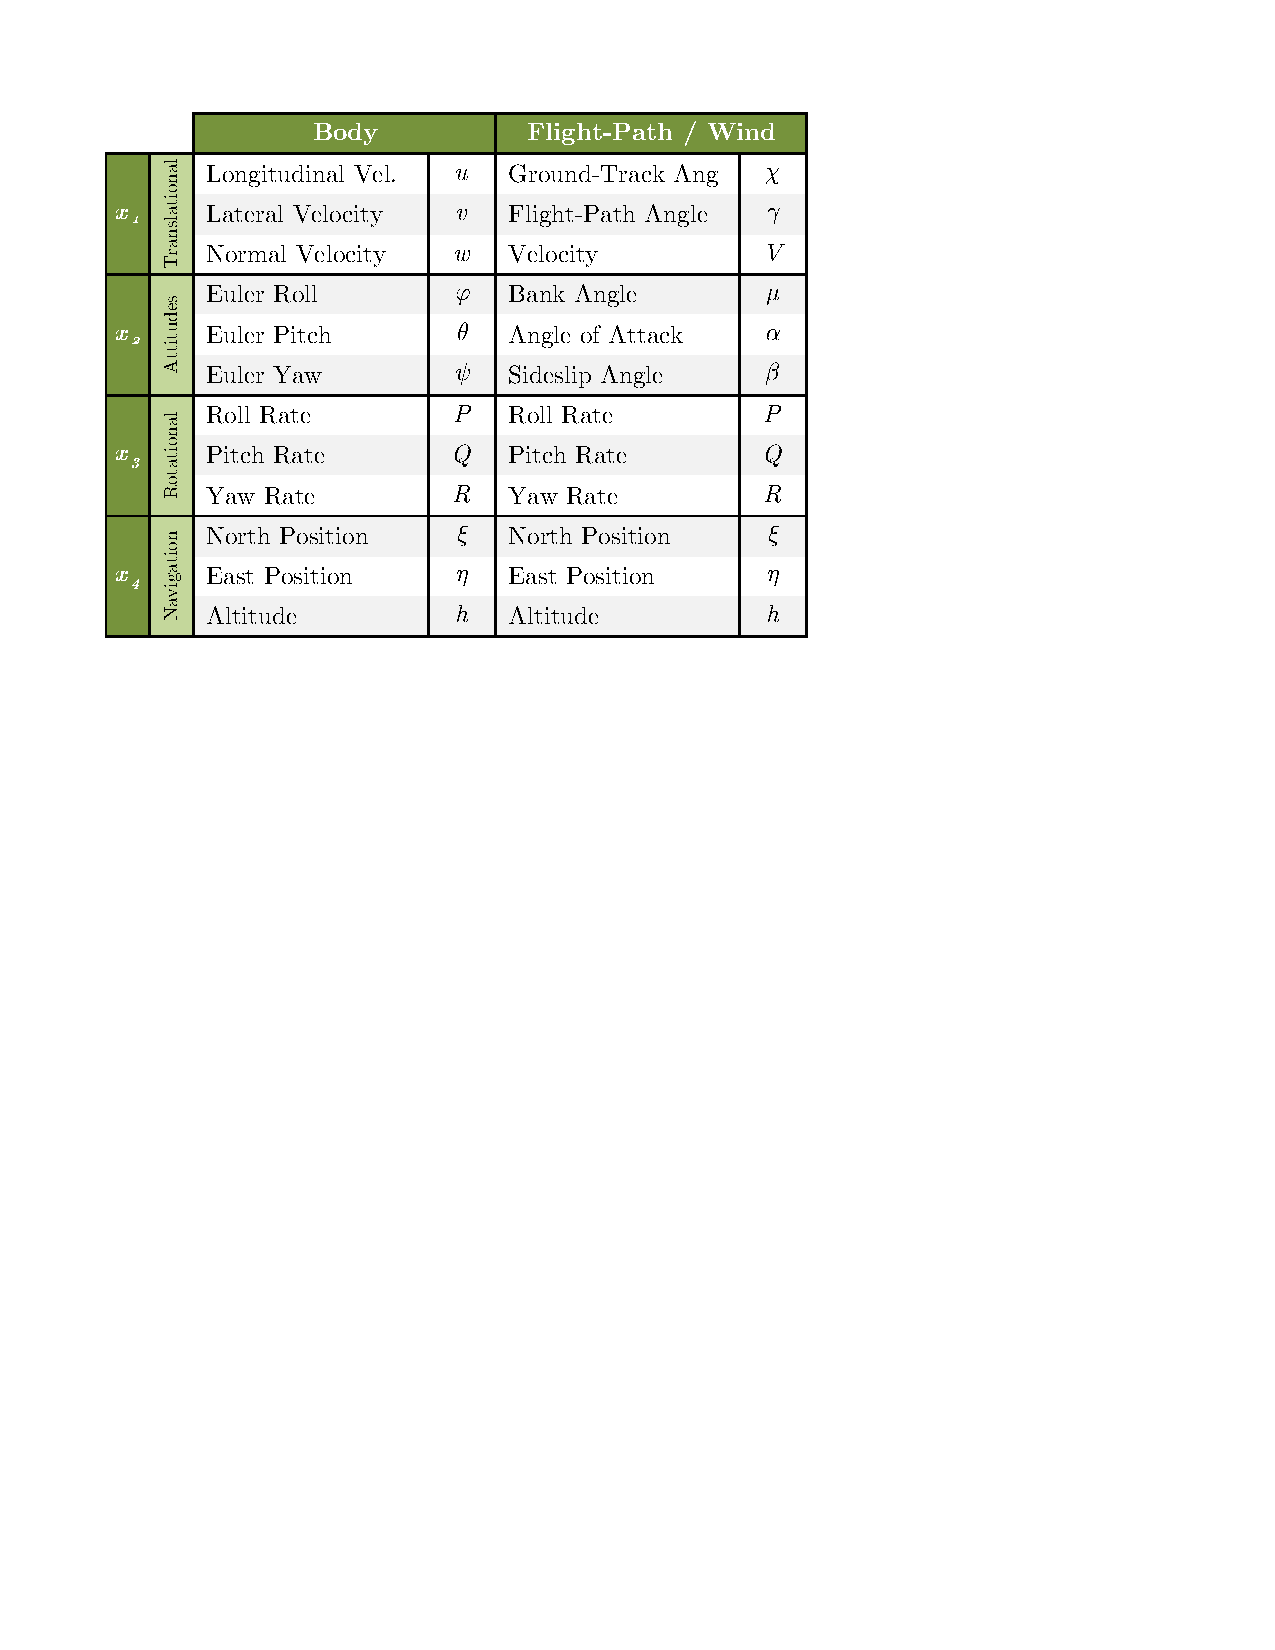
\includegraphics[scale=1,clip=true, viewport=0.5in 6.75in 5.5in 10.25in]{tables/tbl_state_vars.pdf}
			}
			\label{tab: state_vars} 
			
			\\ \\
					
			{\begin{minipage}[t]{0.5\linewidth}
			\textbf{Body}
			\begin{itemize}[labelindent=5pt,leftmargin=*,noitemsep,nosep]%
				\raggedright
				\item 3 components of attitude to specify orientation relative to the gravity vector
				\item 3 components of velocity to specify translational kinetic energy \newline ~
				\item 3 components of angular velocity to specify rotational kinetic energy
				\item 3 components of position to specify potential energy in earth's gravity field
			\end{itemize}
			\end{minipage}
			\hspace{0.025\linewidth}
			\begin{minipage}[t]{0.5\linewidth}
			\textbf{Flight Path / Wind}
			\begin{itemize}[labelindent=5pt,leftmargin=*,noitemsep,nosep]%
				\raggedright
				\item 3 components of attitude to specify orientation relative to the velocity vector
				\item 1 component of velocity magnitude, 2 components of velocity direction to specify translational kinetic energy
				\item 3 components of angular velocity to specify rotational kinetic energy
				\item 3 components of position to specify potential energy in earth's gravity field
			\end{itemize}
			\end{minipage}
			\label{list: state_vars}}
			
		\end{tabular}
	
	\end{table}

\noindent Again the flight path controller herein will only be using the first three subsets of \autoref{tab: state_vars}:

	\begin{align}
		\vect{x} \quad=\quad 
		\left[ \begin{array}{c} \vect{x}_1 \\ \vect{x}_2 \\ \vect{x}_3  \end{array} \right] \quad=\quad 
		\left[ \begin{array}{c} \left( \chi 	\; \gamma 	\; V 		\right)^T \\ 
								\left( \mu 		\; \alpha 	\; \beta 	\right)^T \\ 
								\left( P 		\; Q 		\; R 		\right)^T \end{array} \right] \quad
		\begin{array}{r} \text{Translational}	\\ \text{Attitude} \\ \text{Rotational} \end{array}
		\label{eqn: x}
	\end{align}

%\begin{table}[htbp]
%	\centering
%	\caption{Choices for State Variables}
%	\begin{tabular}{|p{2in}|p{.5in}||p{2in}|p{.5in}|}
%	    \hline
%	    \multicolumn{2}{|p{2.5in}||}{\textbf{Body}} & \multicolumn{2}{p{2.5in}|}{\textbf{Wind / Flight-Path}}\\
%	    \hline
%	    Roll Rate 				& p     	& 	Roll Rate 			& p 		\\
%	    Pitch Rate 				& q     	& 	Pitch Rate 			& q 		\\
%	    Yaw Rate 				& r     	& 	Yaw Rate 			& r 		\\
%	    Longitudinal Velocity 	& u     	& 	Velocity 			& V 		\\
%	    Lateral Velocity 		& v     	& 	Sideslip Angle 		& $\beta$ 	\\
%	    Normal Velocity 		& w     	& 	Angle of Attack 	& $\alpha$ 	\\
%	    Euler Roll Angle 		& $\phi$ 	& 	Bank Angle 			& $\mu$ 	\\
%	    Euler Pitch Angle 		& $\theta$	& 	Flight-Path Angle 	& $\gamma$ 	\\
%	    Euler Yaw Angle 		& $\psi$ 	& 	Heading Angle 		& $\chi$ 	\\
%	    \hline
%	\end{tabular}
%	\label{tab: state_vars}
%\end{table}
%
\subsection{Reference Frames}
\label{subsec: ref}
% The perspective...
Just as language is needed to express thoughts, a reference frame is necessary to convey motion. The relationship between an object and the space it resides in is relative; choosing a reference frame, or coordinate system, enables an observer to describe the motion of an object over time. Selecting an appropriate reference frame can greatly simplify the description of this relationship.

%TODO: Scrap this shitty example, or clean her up
%(A historical example being the 16th century controversy over heliocentrism - the idea that our sun is the center of our \textit{universe}. Before Galileo's telescope findings, people naturally considered the earth an absolutely fixed reference frame as they observed the sun rotate around them. They refused to believe earlier estimates by Copernicus that claimed the earth was rotating about its axis at hundreds of miles per hour \textit{and} orbiting the sun at miles per second. They couldn't feel motion therefore couldn't comprehend it! Not only was the reference frame wrong... Choosing the proper reference frame allows us simplify equations of motion and apply newton's laws. It was Copernicus that realized equations used to determine planet's orbits weren't accurate under the current model****CITE THIS.)

	\begin{ass}
	Earth is an inertial reference frame.
	\label{ass: inertial}
	\end{ass}

\noindent When earth is considered as an inertial frame of reference, one that is \textit{fixed} or moving at a constant velocity (non-rotating and non-accelerating) relative to earth, it permits accurate short-term control and navigation analysis. Conversely, an inertial frame of reference is unacceptable for air vehicles that require long-term navigation, especially for high-speed flight, or extra-atmospheric operation; for most UAVs this assumption is fairly accurate however. As this situation dictates, there are numerous reference systems in aerospace applications. The frames applicable to the equations of motion derivation herein are: body, stability, wind or flight-path, and earth-centered-inertial or earth-fixed. Additionally, north-east-down or local-tangent-plane, vehicle-carried-vertical, and earth-centered-earth-fixed frames will be covered. All coordinate systems follow the right hand rule and are orthogonal.
%
	\begin{figure}[H]
		\centering
		%viewport arguments are the lower-left and upper-right coordinates for the area you want to crop
		\subfloat[Body to Stability Axes]{\label{fig: ref_body_stab}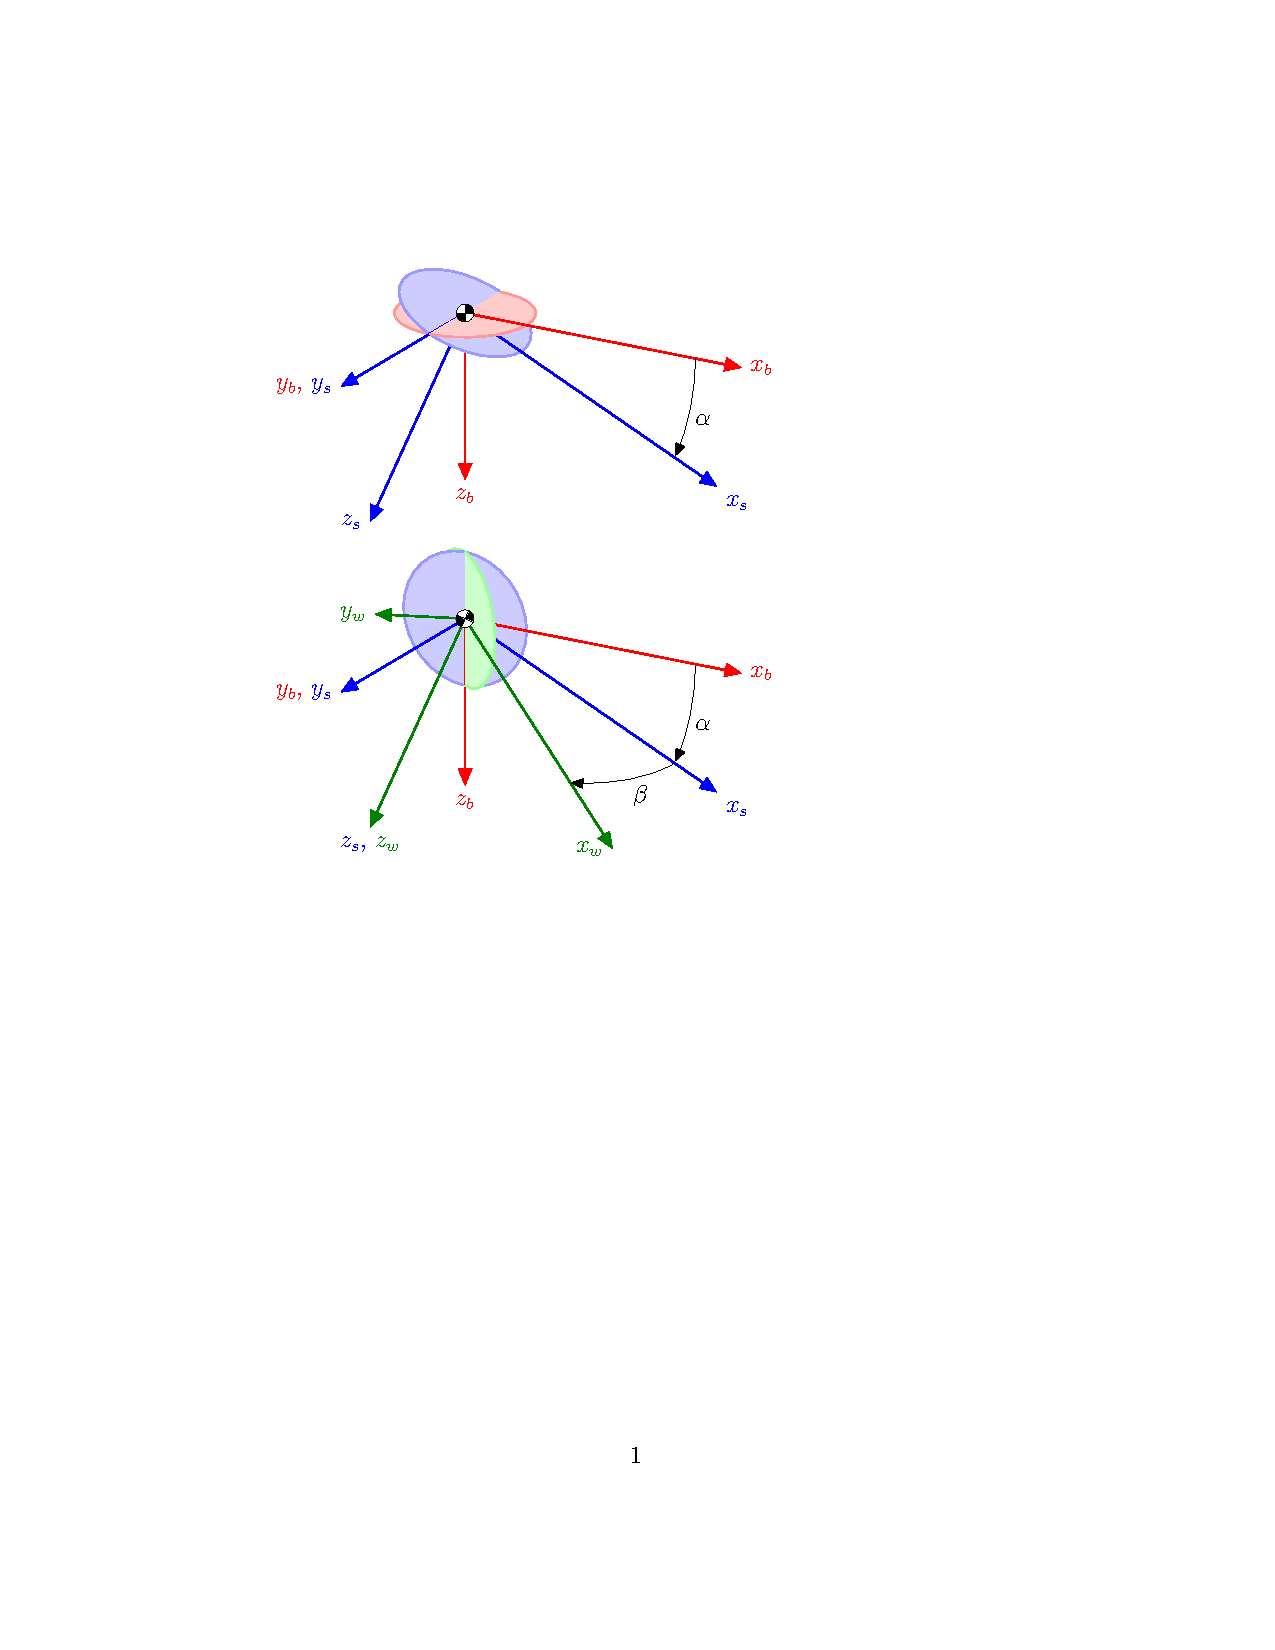
\includegraphics[clip=true, viewport=1.75in 7.35in 5.5in 9.25in,width=0.5\textwidth]{figs/fig_relwind_novec.pdf}}
		\subfloat[Stability to Wind Axes]{\label{fig: ref_stab_wind}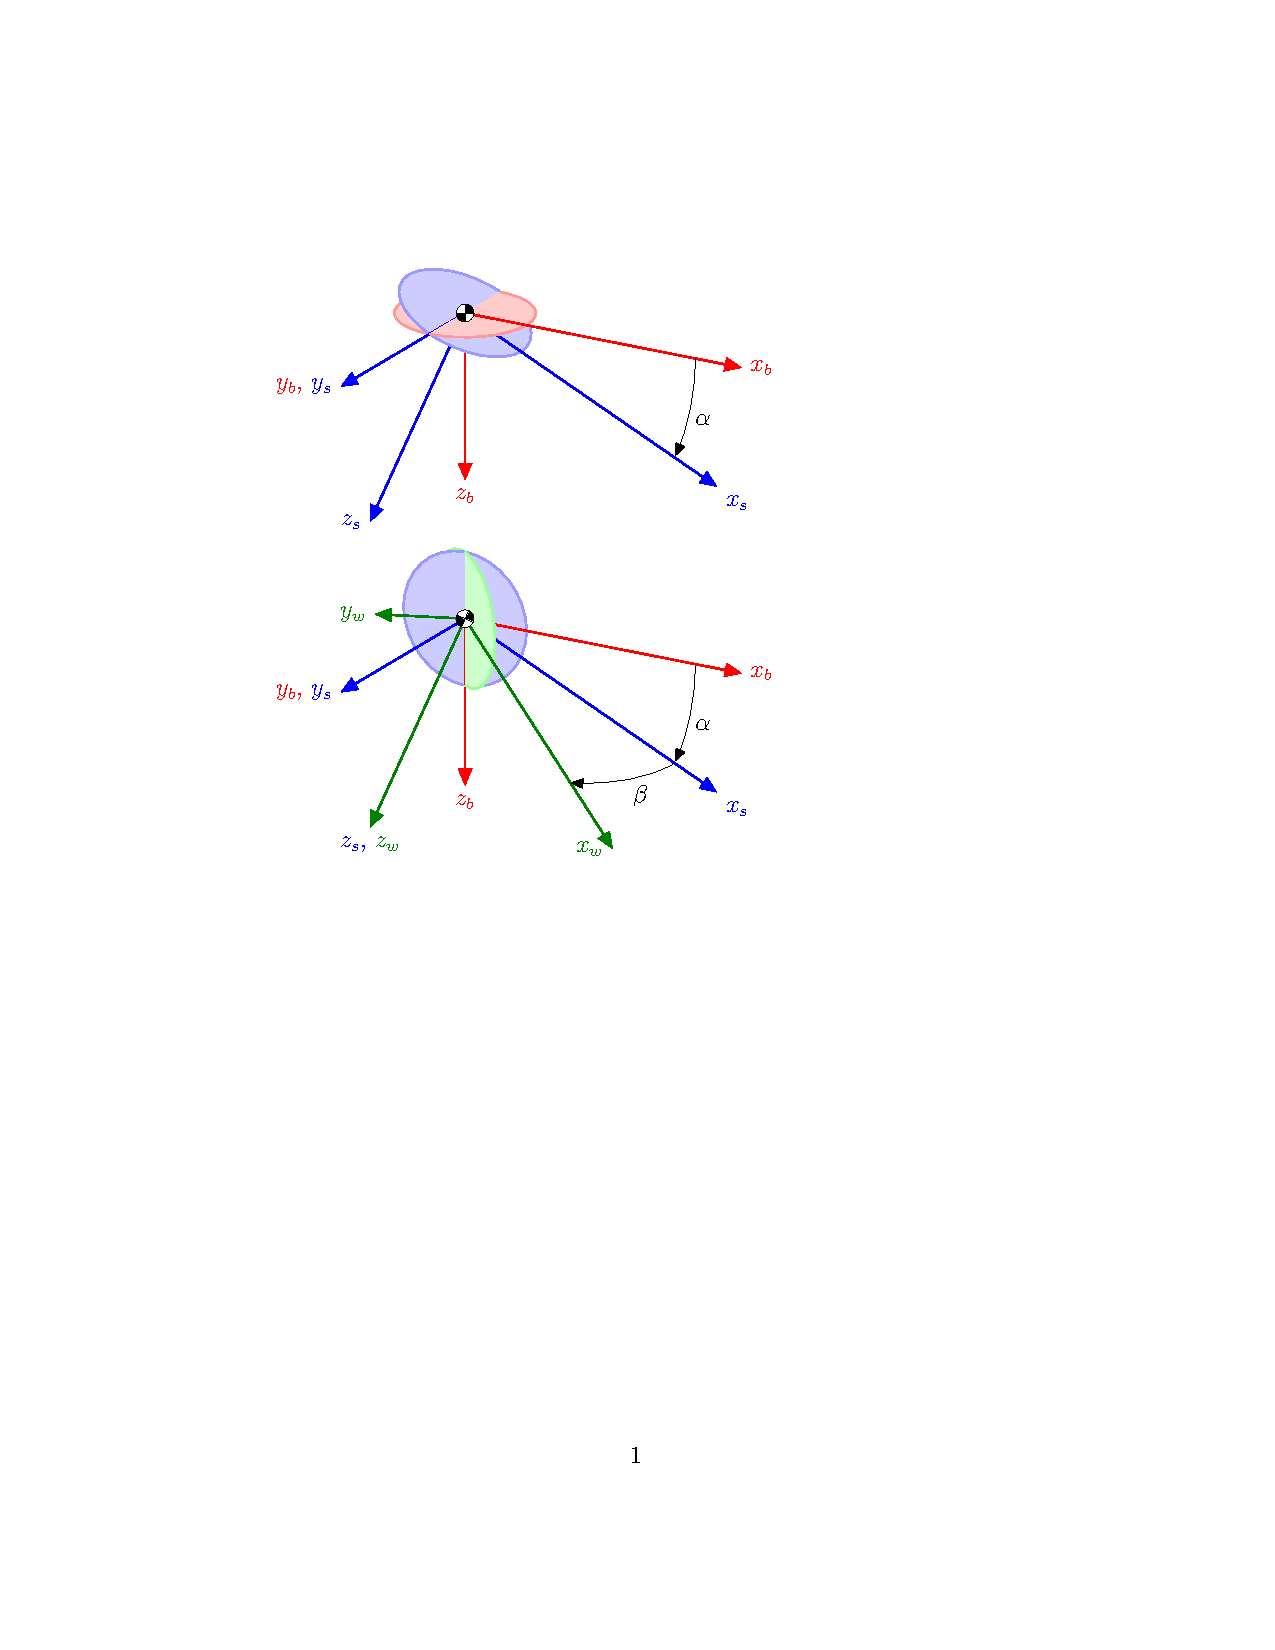
\includegraphics[clip=true, viewport=1.75in 5.25in 5.5in 7.4in,width=0.5\textwidth]{figs/fig_relwind_novec.pdf}}
		\caption{Air Vehicle Reference Frames}
		\label{fig: ref_body_stab_wind}
	\end{figure}

Body, stability, and wind axes are attached to the airframe at the center of gravity as depicted in \autoref{fig: ref_body_stab_wind}. By convention, body axis $x_b$ points out the nose, $y_b$ out the right wing, and $z_b$ down the bottom of the aircraft. Stability axes are defined by a rotation of the body axes in the $x_b$-$z_b$ plane by an angle-of-attack, $\alpha$, that trims the air vehicle, ie. zero pitching moment; axis $x_s$ points into the direction of steady flow, $y_s = y_b$, and $z_s$ is perpendicular to the $x_{s}$-$y_{s}$ plane in the direction following the right handed sign convention. In wind, or flight-path, axes the $x_w$ axis always points into the relative wind. This is defined by a rotation of the body axes through angle-of-attack and sideslip angle with $z_w = z_s$ and $y_w$ following the right hand rule as shown in \autoref{fig: relative_wind}:
	\begin{figure}[H]%
		\centering%
		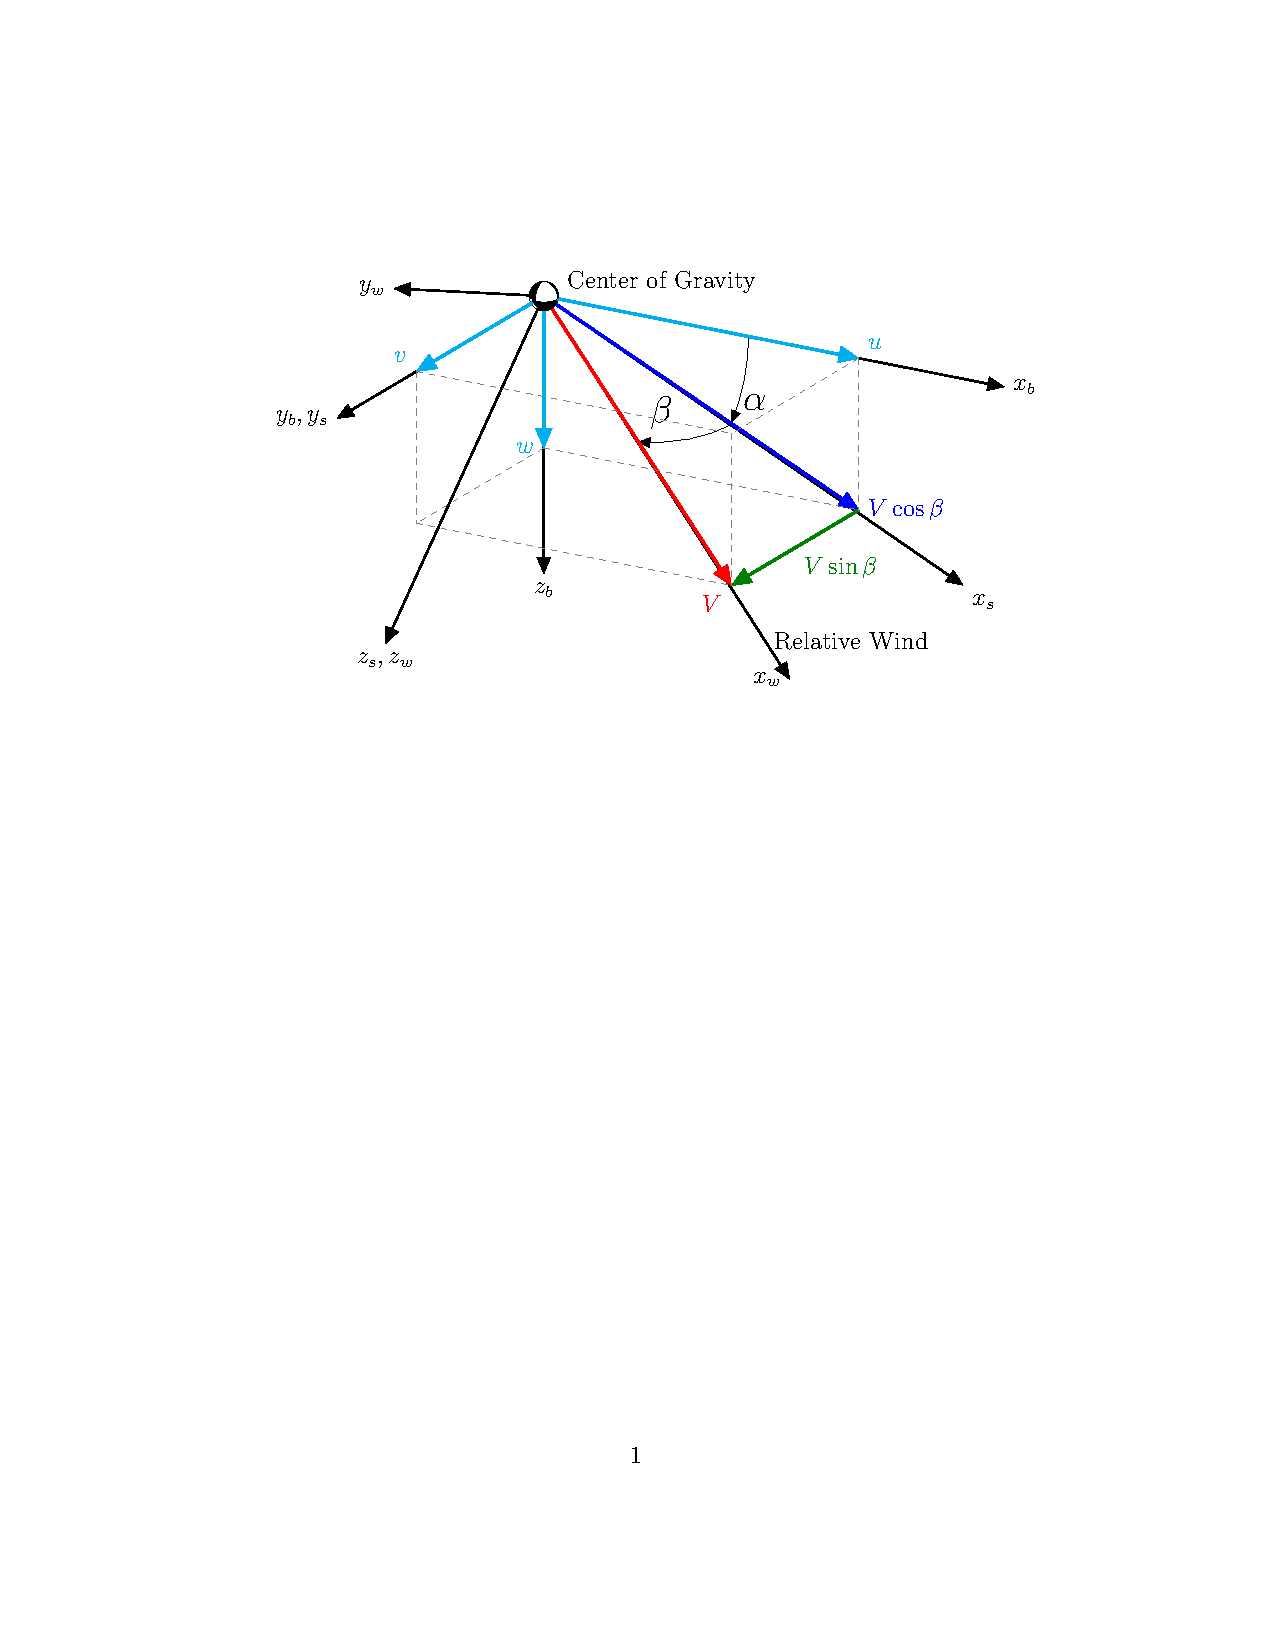
\includegraphics[clip=true, viewport=1.75in 6.35in 7in 9.25in,scale=.8]{figs/fig_relwind.pdf} %
		\caption{Axis Relationships: Body, Stability, and Wind Axes}%
		\label{fig: relative_wind}%
	\end{figure}%
The body state variables can be derived from the flight-path state variables as shown in \citet{WL-TR-96-3099}, recall \autoref{tab: state_vars}:
%
	\begin{gather}
		u		= V\cos\beta\cos\alpha \label{eq: body_u} \\
		v		= V\sin\beta \label{eq: body_v} \\
		w		= V\cos\beta\sin\alpha \label{eq: body_w} \\
		\phi	= \tan^{-1} \left( \frac{\cos\gamma\sin\mu\cos\beta-\sin\gamma\sin\beta}{-\cos\gamma\sin\mu\sin\alpha\sin\beta+\cos\gamma\cos\alpha\cos\mu-\sin\gamma \sin\alpha\cos\beta} \right) \label{eq: body_phi} \\
		\theta	= \sin^{-1} \left( \cos\gamma\sin\mu\cos\alpha\sin\beta+\cos\gamma\cos\mu \sin\alpha+\sin\gamma\cos\alpha\cos\beta \right) \label{eq: body_theta} \\
		\resizebox{.9\hsize}{!}{$
		\psi 	= \tan^{-1} \left\lbrace \frac{ \left( \sin\mu \sin\alpha - \cos\alpha \cos\mu \sin\beta \right) \cos\chi + \left[ \cos\gamma \cos\alpha \cos\beta -\sin\gamma \left( \sin\alpha \cos\mu +\sin\beta \cos\alpha \sin\mu \right) \right] \sin\chi}{- \left( \sin\mu \sin\alpha - \cos\alpha \cos\mu \sin\beta \right) \sin\chi + \left[ \cos\gamma \cos\alpha \cos\beta - \sin\gamma \left(\sin\alpha \cos\mu + \sin\beta \cos\alpha \sin\mu \right) \right] \cos\chi} \right\rbrace$} \label{eq: body_psi}
	\end{gather}
	\nomenclature[-]{$u$, $v$, $w$}{Longitudinal, Lateral, and Normal Velocities\nomunit{ft/s}}% % %  N O M E N C L A T U R E  % % %
	\nomenclature[*u]{$\phi$, $\theta$, $\psi$}{Roll, Pitch, and Yaw Angles\nomunit{deg}}% % %  N O M E N C L A T U R E  % % %

Flight-path variables may be derived from the body state variables as follows, again refer to \citep{WL-TR-96-3099} and recall \autoref{tab: state_vars}:
%
	\begin{gather}%
		V		=\sqrt{u^{2}+v^{2}+w^{2}} \label{eq: wind_v}\\
		\alpha 	=\tan^{-1}\left( \displaystyle \frac{w}{u} \right) \label{eq: wind_alpha} \\
		\beta	=\sin^{-1} \left( \displaystyle \frac{v}{\sqrt{u^{2}+v^{2}+w^{2}}} \right) \label{eq: wind_beta} \\
		\mu		=\tan^{-1} \left[ \displaystyle \frac{uv\sin\theta+ \left(u^2+w^2 \right) \sin\phi \cos\theta -vw\cos\phi \cos\theta}{\sqrt{u^2+v^2+w^2} \left( w\sin\theta + u\cos\phi \cos\theta \right)} \right] \label{eq: wind_mu} \\
		\gamma	=\sin^{-1} \left( \displaystyle \frac{u\sin\theta-v\sin\phi\cos\theta-w\cos\phi\cos\theta}{\sqrt{\mathrm{u}^{2}+v^{2}+w^{2}}} \right)
		\label{eq: wind_gam} \\
		\resizebox{.8\hsize}{!}{$ \chi=\tan^{-1} \left[ \frac{u\cos\theta\sin\psi+v \left( \sin\phi\sin\theta\sin\psi+\cos\phi\cos\psi \right) + w \left( \cos\phi \sin\theta \sin\psi - \sin\phi \cos\psi \right)}{u\cos\theta \cos\psi + v \left( \sin\phi \sin\theta \cos\psi - \cos\phi \sin\psi \right) + w \left( \cos\phi \sin\theta \cos\psi + \sin\phi \sin\psi \right)} \right]$} \label{eq: wind_chi}
	\end{gather}%
	\nomenclature[+]{$V$}{Airspeed\nomunit{ft/s}}% % %  N O M E N C L A T U R E  % % %
	\nomenclature[*a]{$\alpha$}{Angle of Attack\nomunit{deg}}% % %  N O M E N C L A T U R E  % % %
	\nomenclature[*b]{$\beta$}{Angle of Sideslip\nomunit{deg}}% % %  N O M E N C L A T U R E  % % %
	\nomenclature[*l]{$\mu$}{Bank Angle\nomunit{deg}}%% % %  N O M E N C L A T U R E  % % %
	\nomenclature[*c]{$\gamma$}{Flight-Path Angle\nomunit{deg}}% % %  N O M E N C L A T U R E  % % %
	\nomenclature[*v]{$\chi$}{Ground-Track Angle\nomunit{deg}}% % %  N O M E N C L A T U R E  % % %

North East Down (NED), also known as Local Tangent Plane (LTP), is positioned on the surface of earth with it's origin vertically aligned to the aircraft's center of gravity. North is parallel to lines of longitude ($\lambda$), east is parallel to lines of latitude ($\phi$), and down completes the right hand rule pointing into earth. Vehicle Carried Vertical (VCV) shares the NED orientation definition, with the exception of a shift in origin from Earth's surface to the vehicle's center of gravity, as the name suggests. 
%
	\begin{figure}[htb]
	  \centering
	  %viewport arguments are the lower-left and upper-right coordinates for the area you want to crop
	  \subfloat[Earth Centered Inertial (Fixed)]{\label{fig: ref_frame_eci}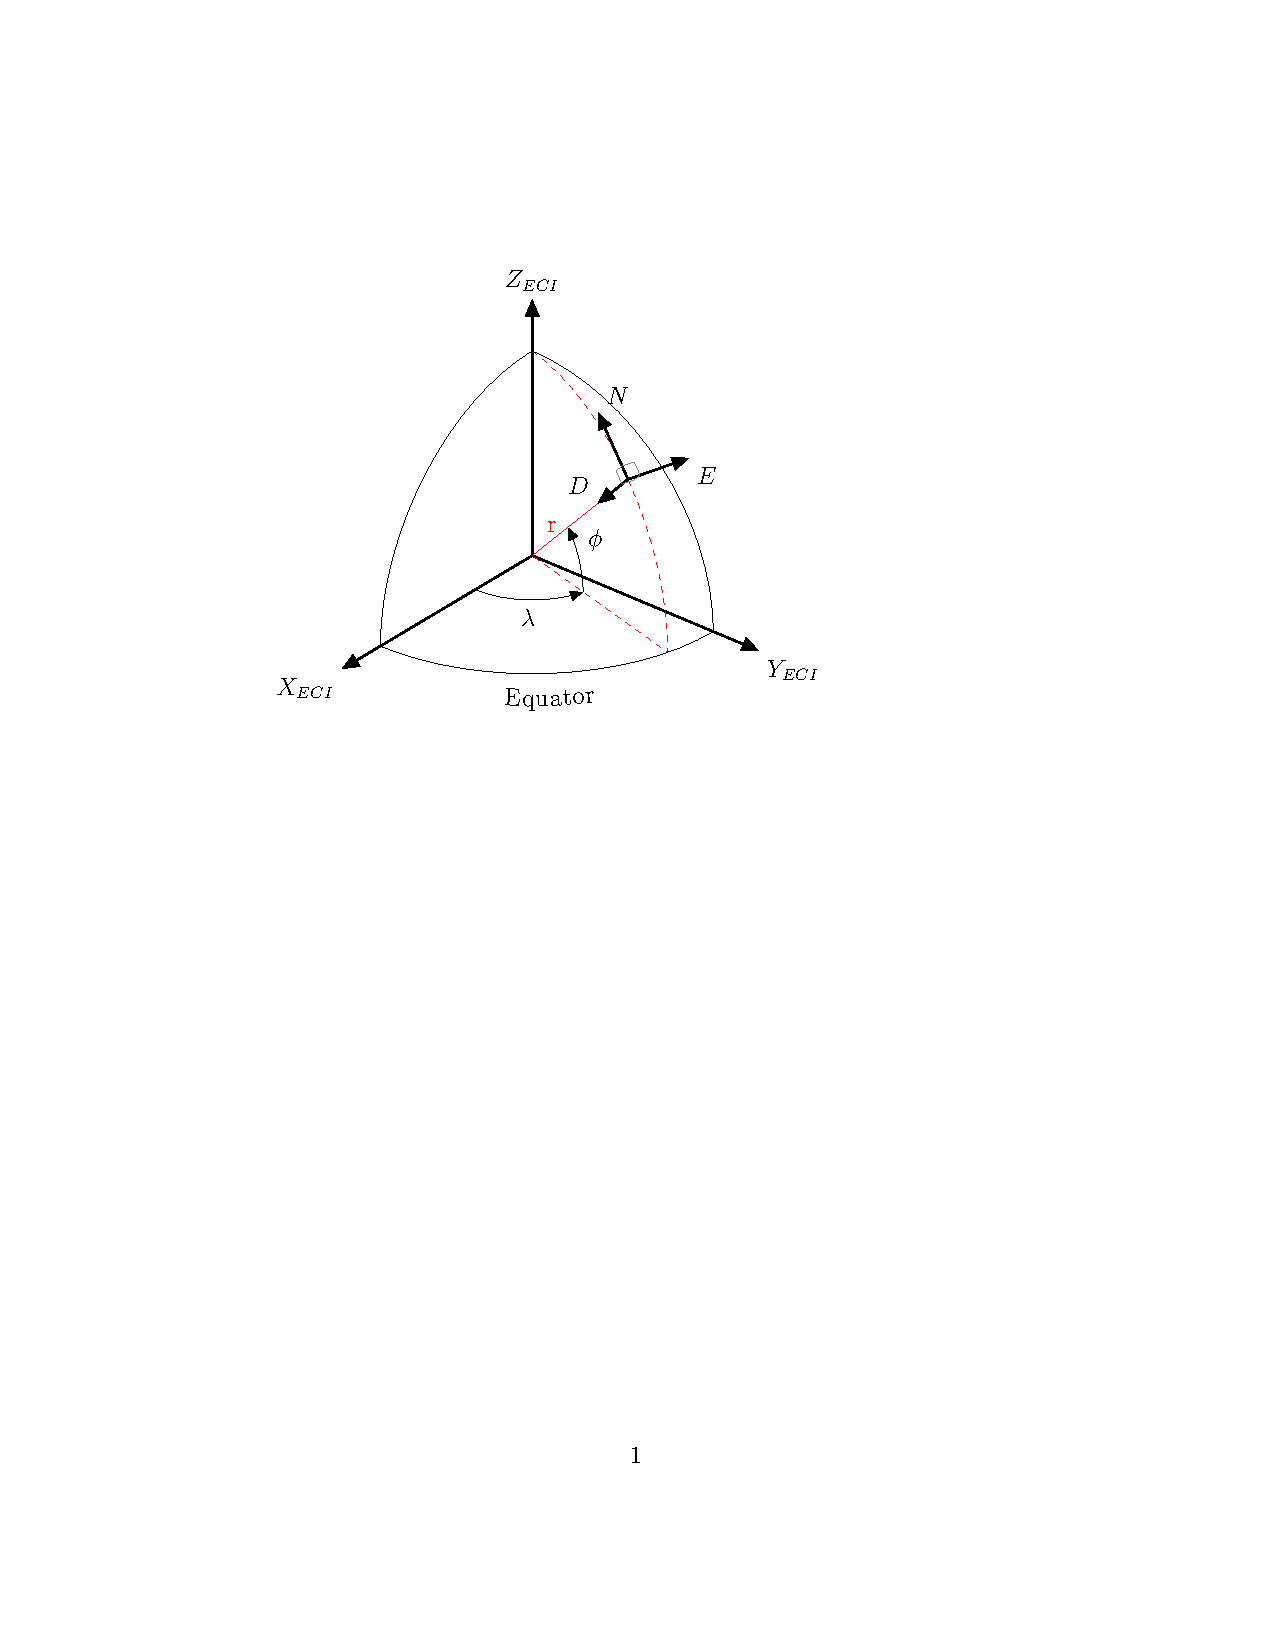
\includegraphics[clip=true, viewport=1.5in 6.25in 5.75in 9.25in,width=0.5\textwidth]{figs/fig_refframe_inertial.pdf}}
	  \subfloat[Earth Centered Earth Fixed (Rotates)]{\label{fig: ref_frame_ecef}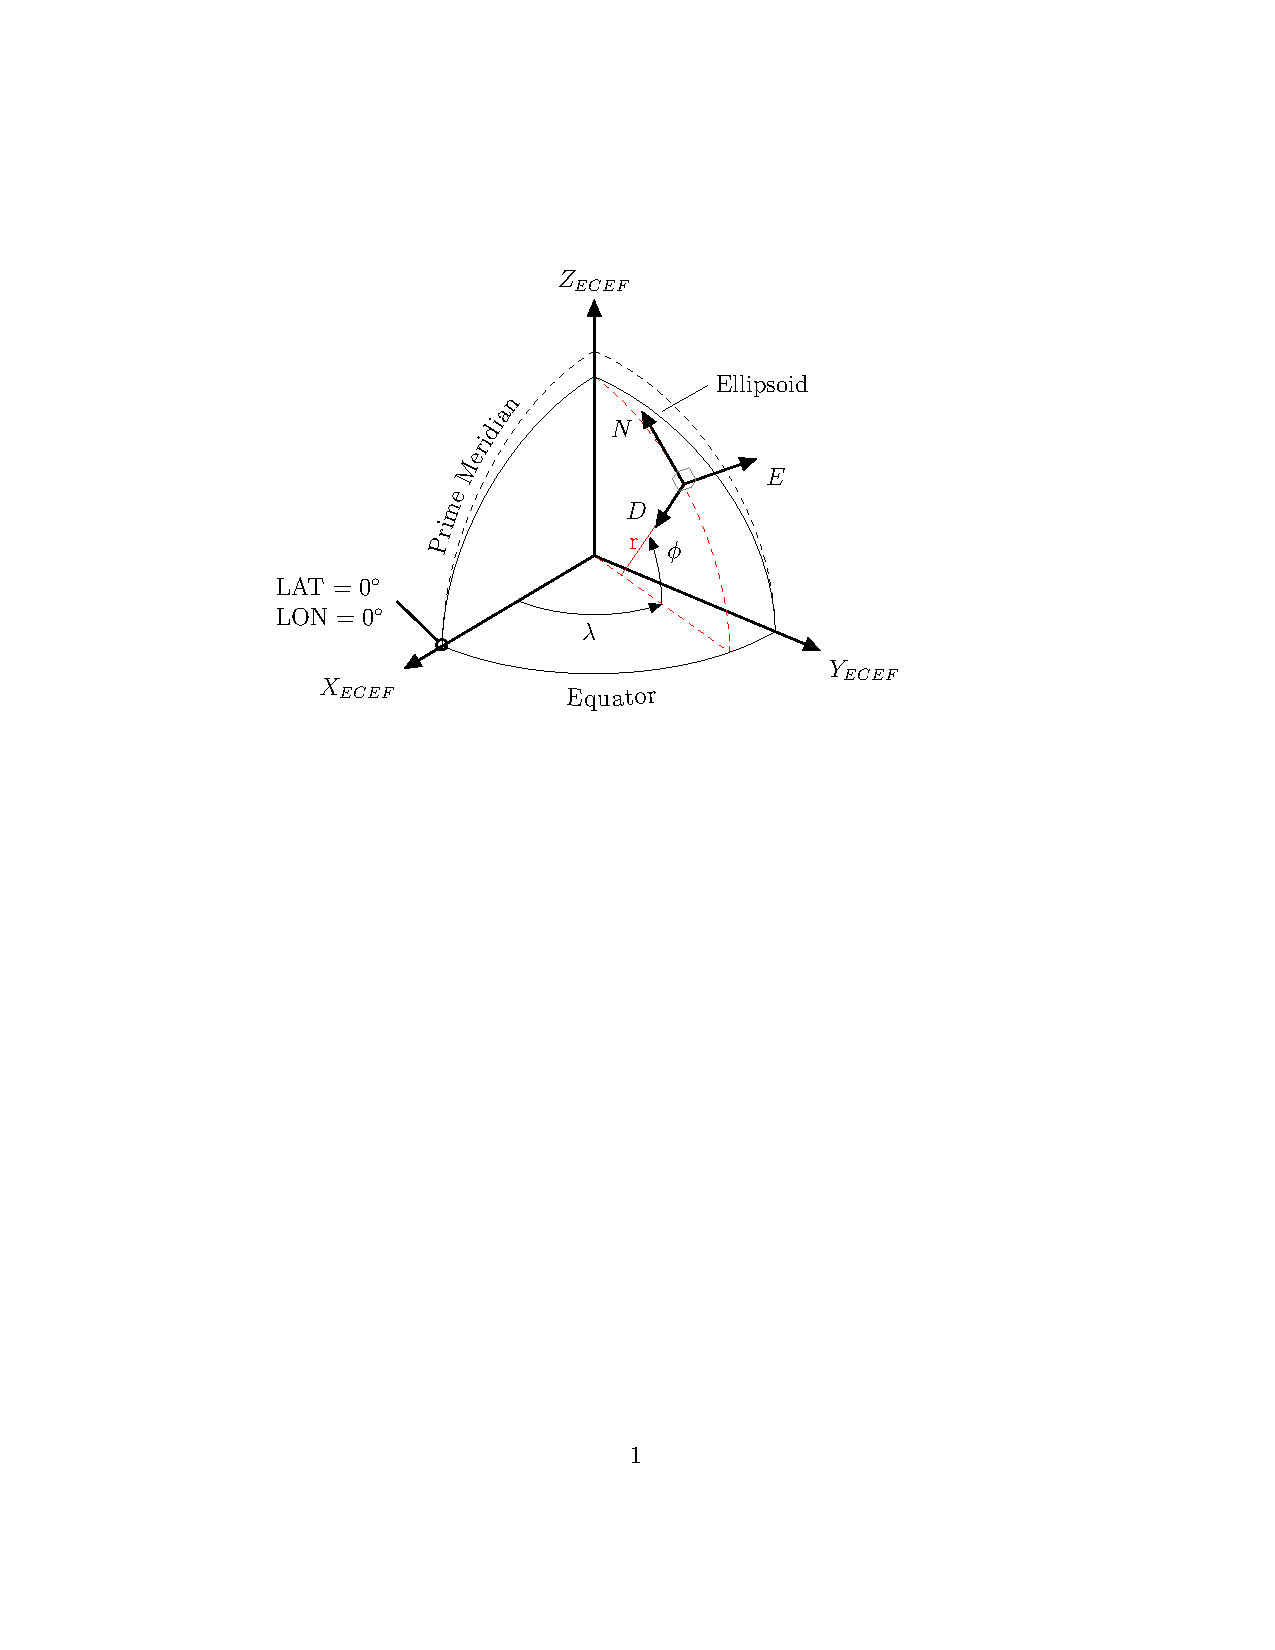
\includegraphics[clip=true, viewport=1.75in 6.25in 6in 9.25in,width=0.5\textwidth]{figs/fig_refframe_ecef.pdf}}
	  \caption{Earth Reference Frames}
	  \label{fig: ref_frames}
	\end{figure}

The Earth Centered Inertial (ECI) frame is considered \textit{fixed} in space with its origin at the center of Earth; it does not rotate with Earth and is oriented to suit the situation. Typically the $z_{ECI}$ axis is aligned along Earth's spin axis pointing toward the North Pole. Consult \citet[Pg. 20]{Stevens1992}, for alternative ECI orientations.
\nomenclature[A]{ECI}{Earth Centered Inertial}% % %  N O M E N C L A T U R E  % % %

Earth Centered Earth Fixed (ECEF) is a non-inertial frame that rotates with earth. This reference system aligns  $x_{ECEF}$ to the intersection of the zero-longitude prime meridian and zero-latitude equator. $y_s$ lies in the equatorial plane and $z_{ECEF}$ points toward the Earth's North Pole. Note how the radius endpoint is not coincident with the center of the ellipsoid; this is because the radius emanates from a plane tangent to the ellipsoid surface. 
\nomenclature[A]{ECEF}{Earth Centered Earth Fixed}% % %  N O M E N C L A T U R E  % % %
%TODO: A variety of ``languages'' will be introduced the succeeding sections, the aircraft state can be expressed in  a multitude of ways, whichever is convenient to the control architecture in place.

\subsection{Direction Cosine Matrices}
\label{subsec: new_dcm}
%The interpreter... Direction Cosine Matrix
If reference frames were languages, direction cosine matrices would be interpreters. It allows a vector's orientation to be expressed as components among relative coordinate systems. As the name suggests, rotations are achieved by defining a matrix of direction cosines that relate \textit{unit vectors} in one axis system to those in another, preserving the length of the rotated vector. The determination of matrix elements may be accomplished by inspection; \citet{McRuer1973} and \citet{Stevens2003} note several general properties for construction of these matrices:
%
	\begin{itemize}[labelindent=\parindent,leftmargin=*,noitemsep,topsep=0pt,partopsep=0pt]%
		\item ``The one is always associated with the axis about which rotation occurs.''
		\item ``The remaining elements in the row and column containing the one are all zeros.''
		\item The remaining main diagonal terms are the cosine of the angle of rotation.
		\item The remaining matrix elements contain the sine of the angle of rotation and are always symmetrically placed relative to the cosine terms; this is done so that zero rotation produces an identity matrix.
		\item ``In the direct right-handed rotation the negative sign always appears in the row above the one (this is to be interpreted as the third row if the one is in the first).''
		\item ``Changing the sign of the rotation angle yields the matrix transpose.''
	\end{itemize}

A coordinate rotation example from the body axis frame, $\vect{F_B}$, to north-east-down frame, $\vect{F_{NED}}$, is illustrated by three plane rotations in \autoref{tab: dcm_plane_rot}.
\nomenclature[+]{$\vect{F}$}{Reference Frame; Force}% % %  N O M E N C L A T U R E  % % %
%
%TODO: Pg 23 Stevens u_vec
\begin{table}[!ht]
  	\centering
  	\caption{Direction Cosine Matrices for Plane Rotations}
    \begin{tabular}{>{\centering\arraybackslash}m{0.45\textwidth}>{\centering\arraybackslash}m{0.45\textwidth}}
	\toprule
		%\label{eq: DCM_Phi}
		\begin{tabular}{>{\centering\arraybackslash}m{.25in}|>{\centering\arraybackslash}m{.5in}>{\centering\arraybackslash}m{.5in}>{\centering\arraybackslash}m{.5in}}
		$C_{\Phi}$ & $x_B$ & $y_B$ & $z_B$\\ 
		\hline
		$x_{\Phi}$ & 1 & 0 & 0 \\
		$y_{\Phi}$ & 0 & $\cos\Phi$ & $\sin\Phi$ \\
		$z_{\Phi}$ & 0 & $-\sin\Phi$ & $\;\;\;\cos\Phi$ \\
		\end{tabular}
	&
		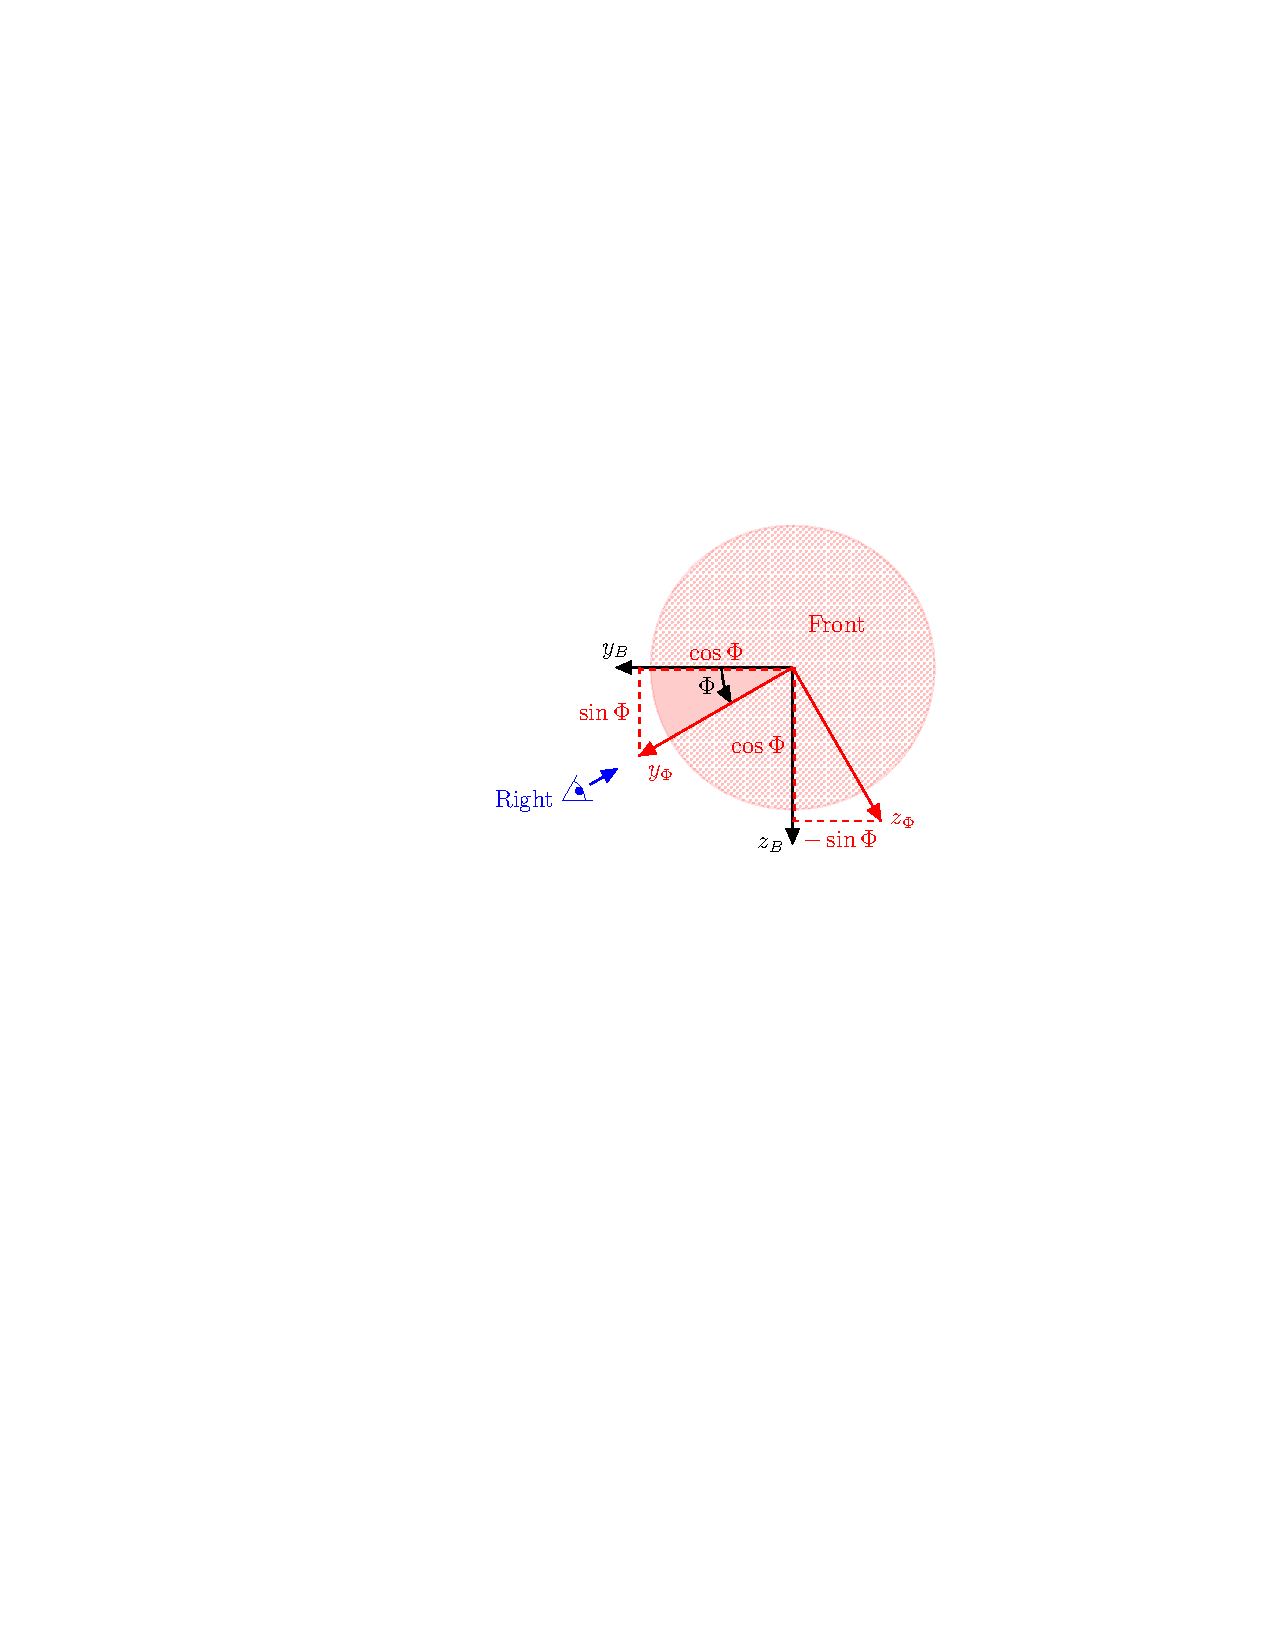
\includegraphics[clip=true, viewport=3.25in 5.25in 6.75in 7.5in, scale=.75]{figs/fig_dcm_2D_1.pdf}
	\\
	\midrule
		\begin{tabular}{>{\centering\arraybackslash}m{.25in}|>{\centering\arraybackslash}m{.5in}>{\centering\arraybackslash}m{.5in}>{\centering\arraybackslash}m{.5in}}
		$C_{\Theta}$ & $x_{\Phi}$ & $y_{\Phi}$ & $z_{\Phi}$\\ 
		\hline
		$x_{\Theta}$ & $\;\;\;\cos\Theta$ & 0 & $-\sin\Theta$ \\
		$y_{\Theta}$ & 0 & 1 & 0 \\
		$z_{\Theta}$ & $\sin\Theta$ & 0 & $\cos\Theta$ \\
		\end{tabular}
	&
		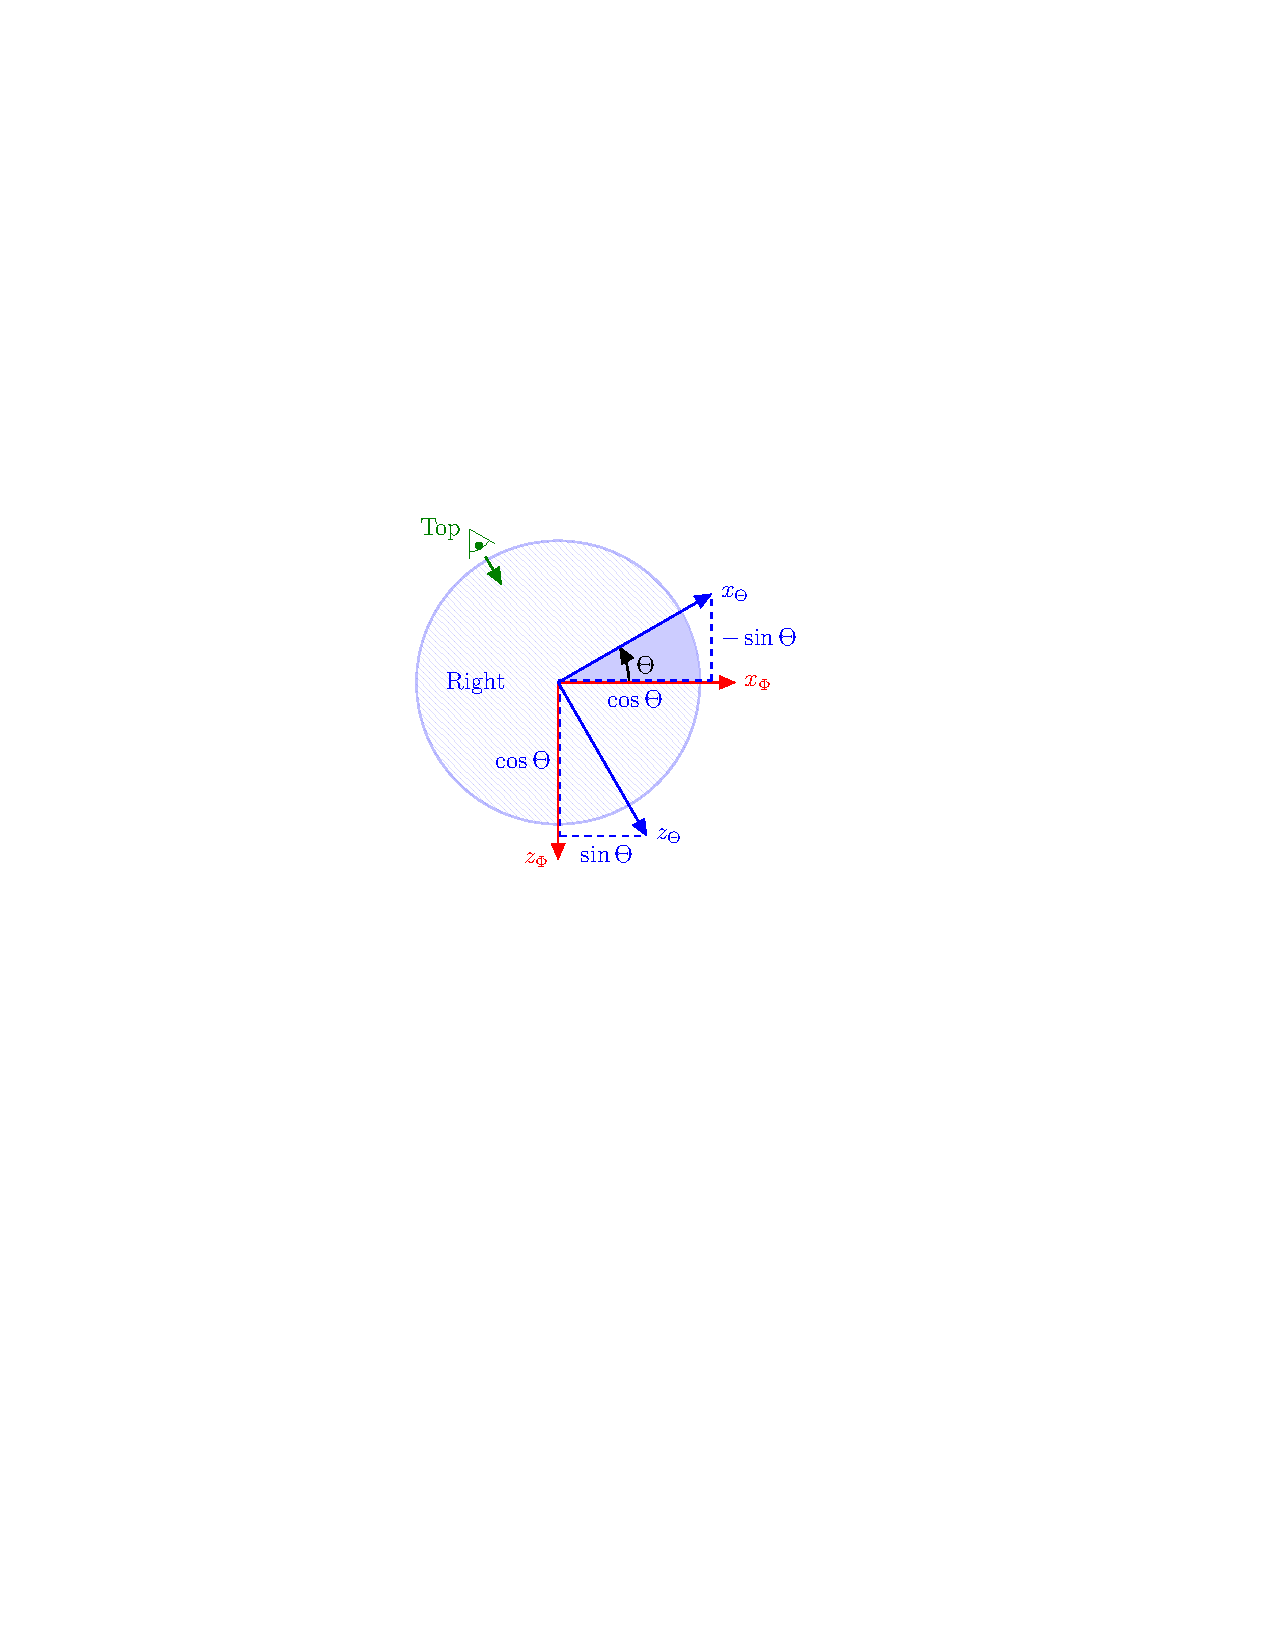
\includegraphics[clip=true, viewport=1.5in 5.2in 5.5in 7.6in, scale=.75]{figs/fig_dcm_2D_2.pdf}
	\\
	\midrule
		%\label{eq: DCM_Psi}
		\begin{tabular}{>{\centering\arraybackslash}m{.25in}|>{\centering\arraybackslash}m{.5in}>{\centering\arraybackslash}m{.5in}>{\centering\arraybackslash}m{.5in}}
		$C_{\Psi}$ & $x_{\Theta}$ & $y_{\Theta}$ & $z_{\Theta}$\\ 
		\hline
		$x_{\Psi}$ & $\cos\Psi$ & $\sin\Psi$ & 0 \\
		$y_{\Psi}$ & $-\sin\Psi$ & $\;\;\;\cos\Psi$ & 0 \\
		$z_{\Psi}$ & 0 & 0 & 1 \\
		\end{tabular}
	& 
		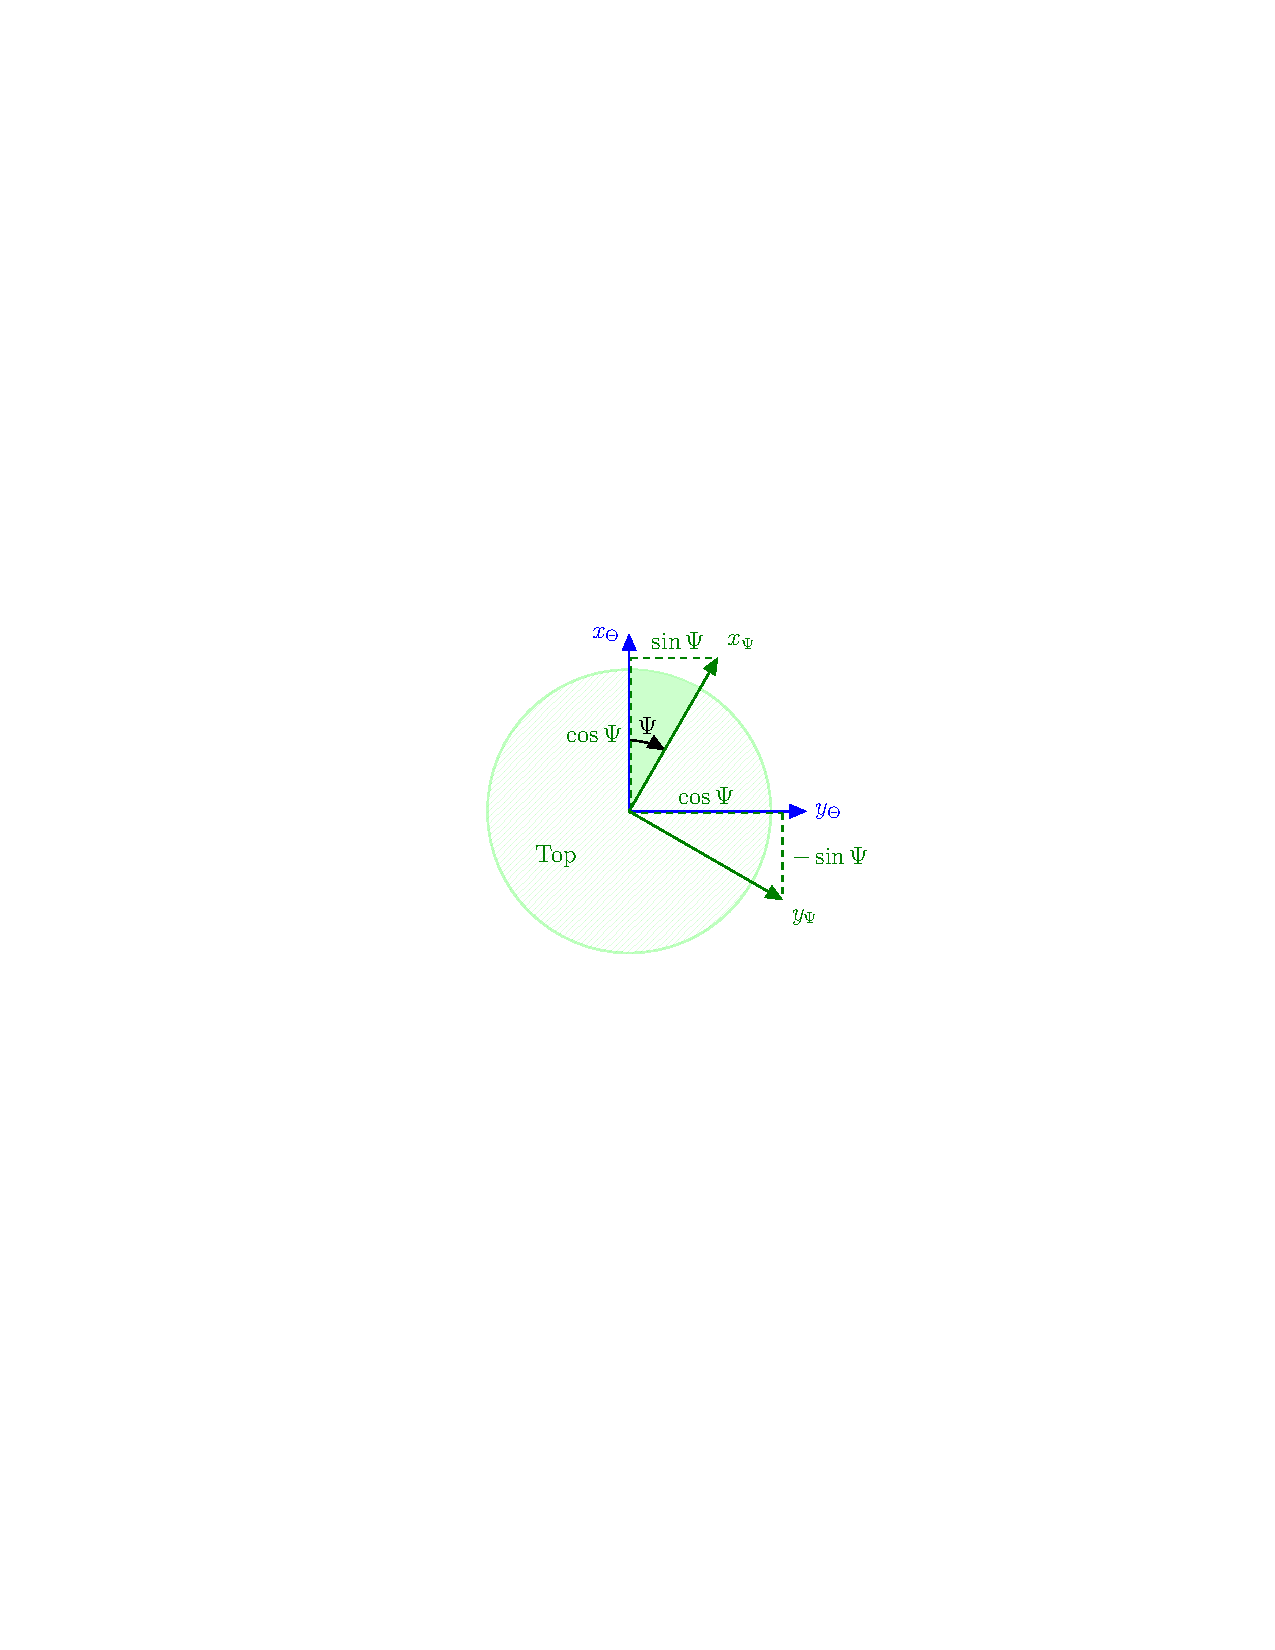
\includegraphics[clip=true, viewport=2in 4.625in 6in 6.875in, scale=.75]{figs/fig_dcm_2D_3.pdf}
	\\
	\bottomrule
    \end{tabular}%
    \label{tab: dcm_plane_rot}
\end{table}%
\nomenclature[+]{$C$}{Direction Cosine Matrix}% % %  N O M E N C L A T U R E  % % %
%
%HORIZONTAL
%\begin{figure}[htb]
%  \centering
%  %http://texblog.net/latex-archive/layout/centering-figure-table/
%  \noindent\makebox[\textwidth]{%
%  \subfloat[Roll Rotation]{\label{fig: dcm_2D_1}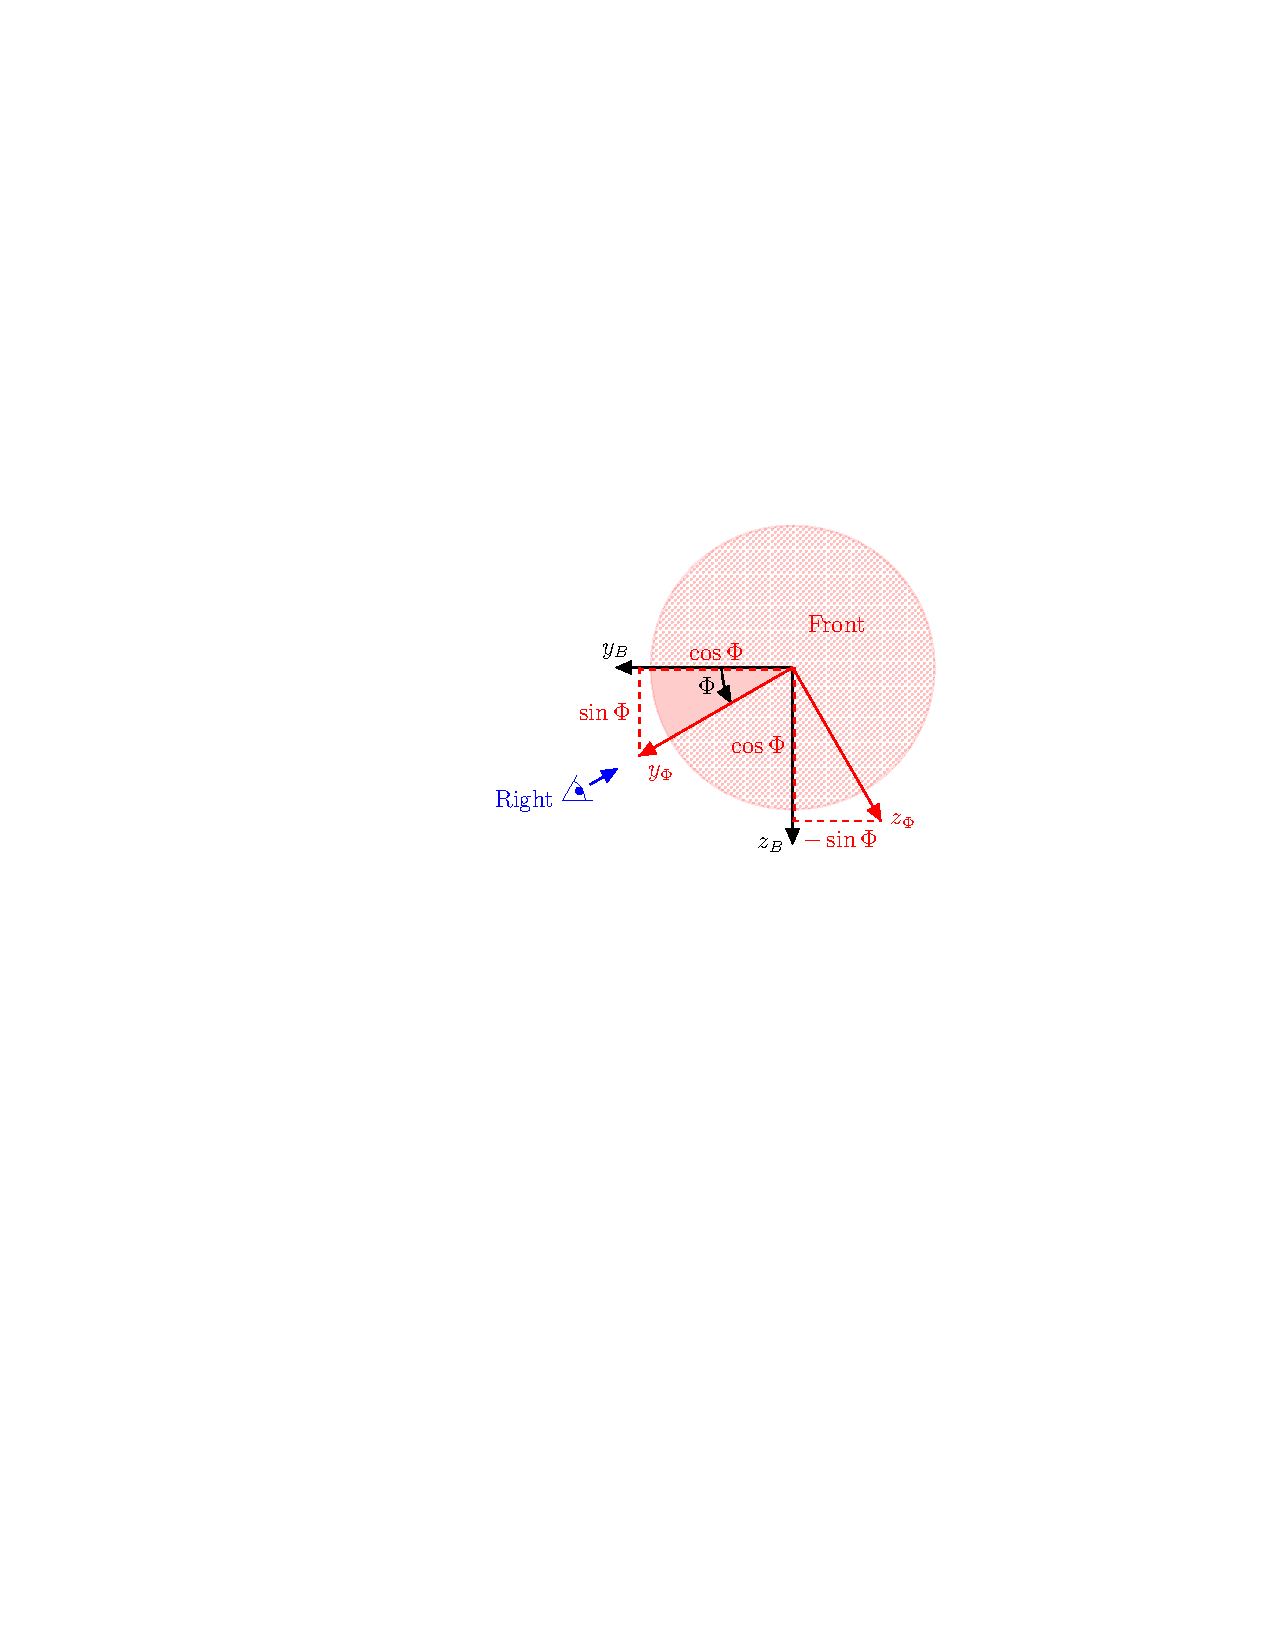
\includegraphics[clip=true, viewport=2.75in 4.5in 6.25in 7.75in, scale=.75]{figs/fig_dcm_2D_1.pdf}}%
%  \subfloat[Pitch Rotation]{\label{fig: dcm_2D_2}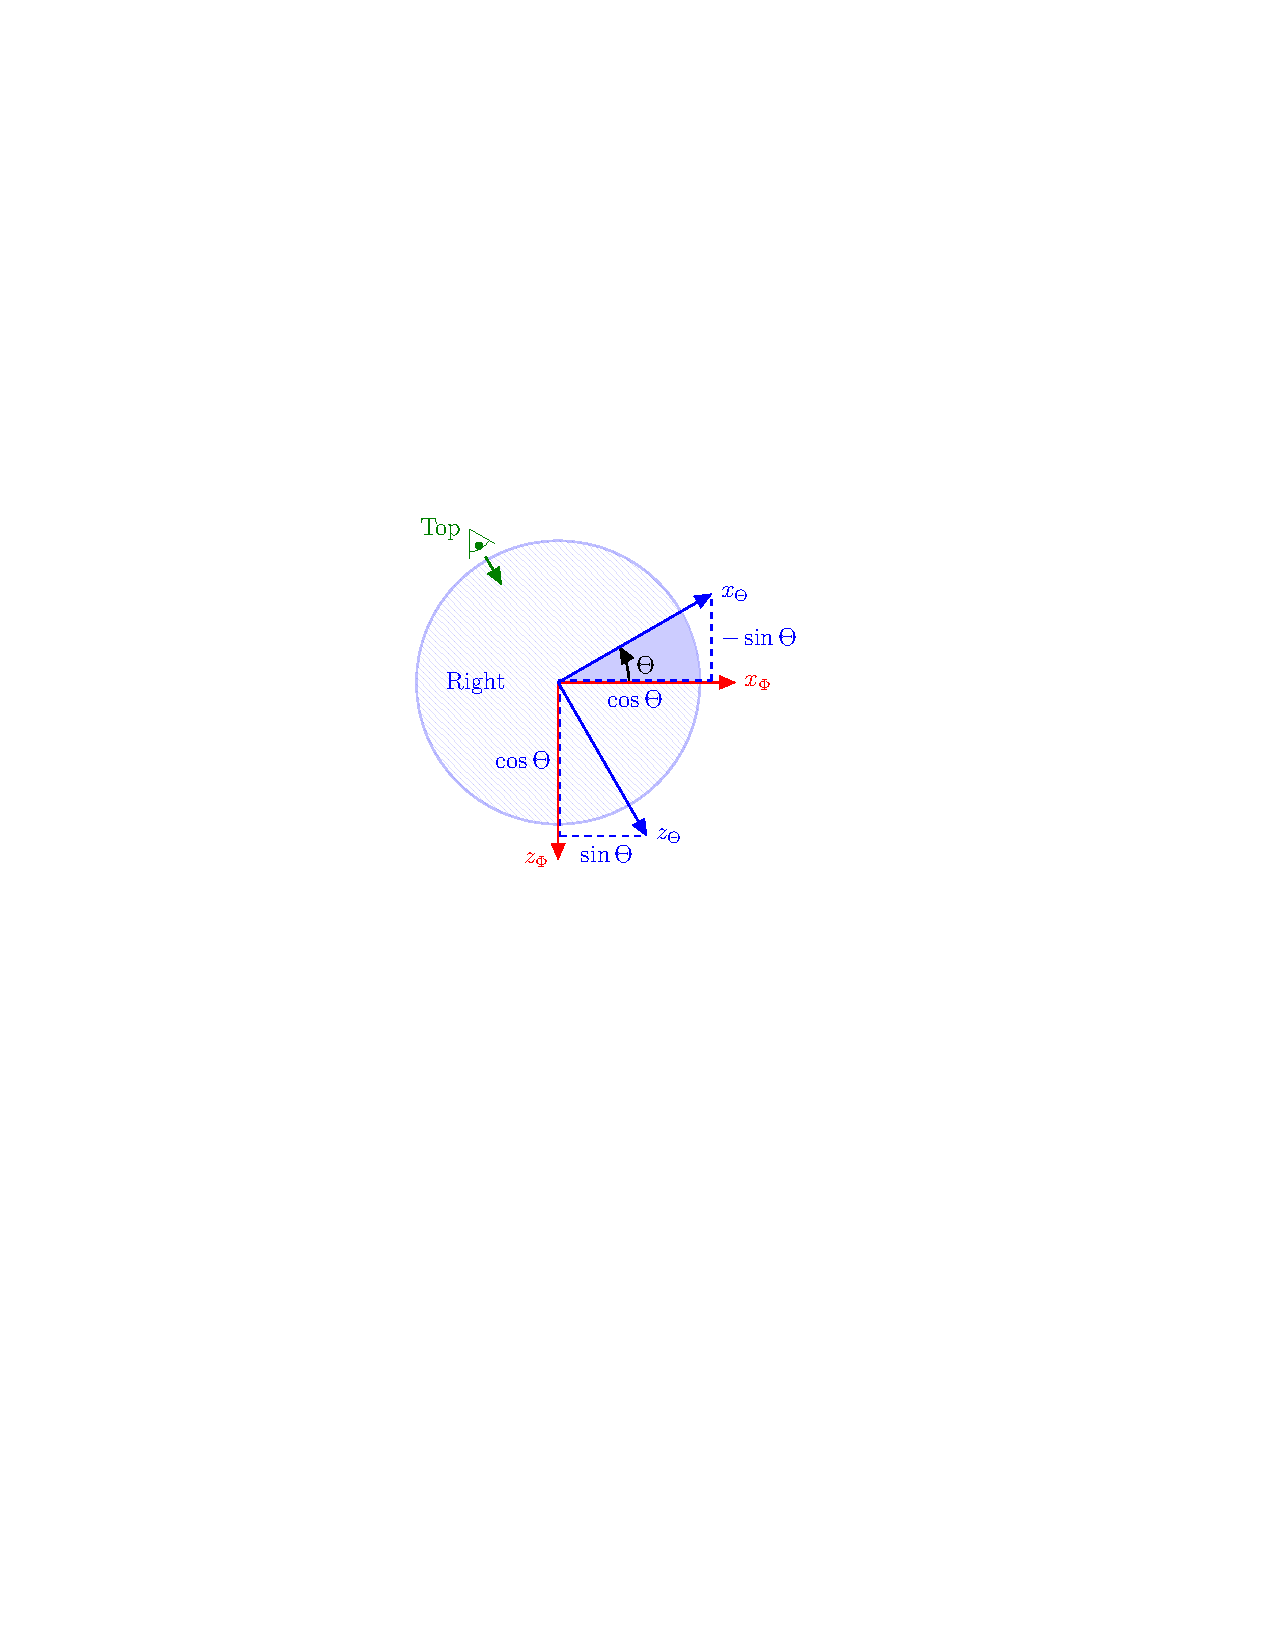
\includegraphics[clip=true, viewport=2.5in 4.5in 6.0in 7.75in, scale=.75]{figs/fig_dcm_2D_2.pdf}}%
%  \subfloat[Yaw Rotation]{\label{fig: dcm_2D_3}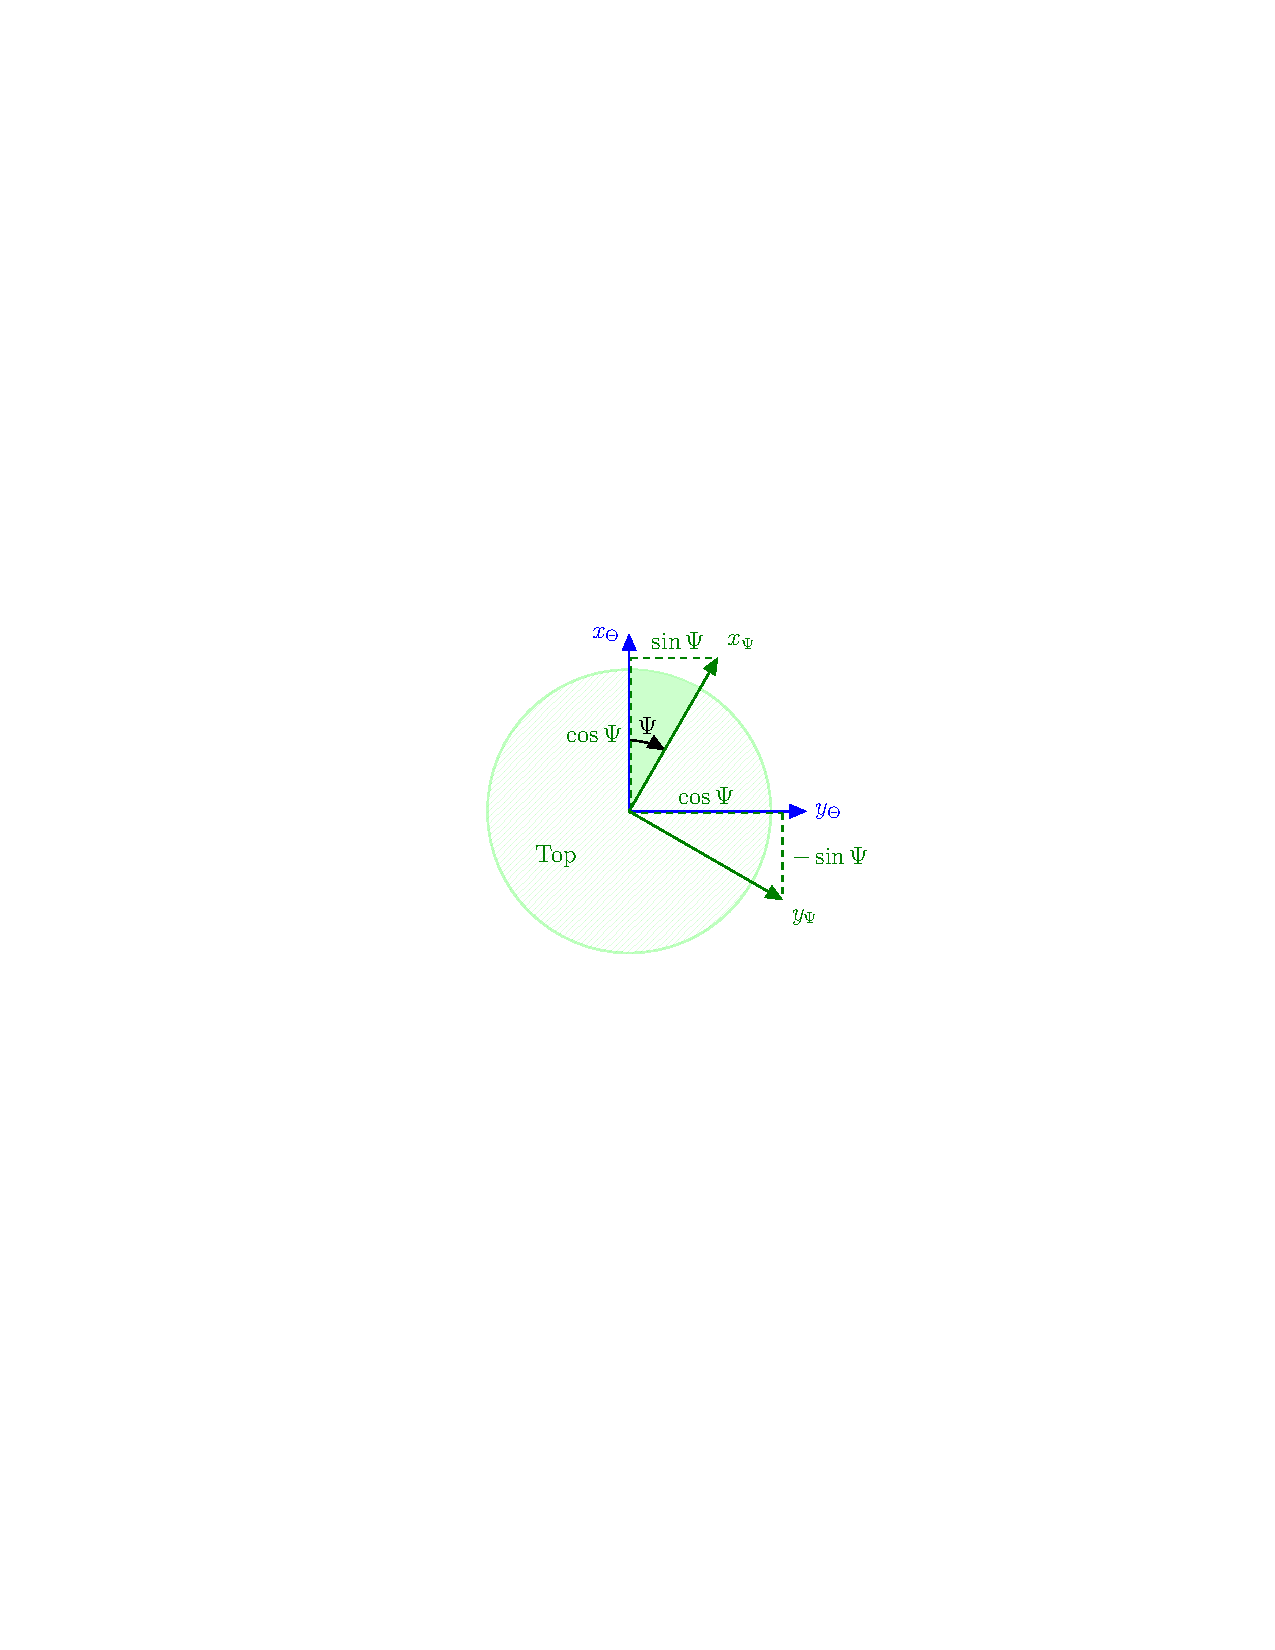
\includegraphics[clip=true, viewport=2.5in 4.5in 6.0in 7.75in, scale=.75]{figs/fig_dcm_2D_3.pdf}}}%
%  \caption{Direction Cosine Matrix Projected Rotations}%
%  \label{fig: dcm_2D}%
%\end{figure}
%VERTICAL
%\begin{wrapfigure}{r}{2in}
%  \vspace{-2in} %shift this bitch up!
%  \centering
%  \subfloat[Roll Rotation]{\label{fig: dcm_2D_1}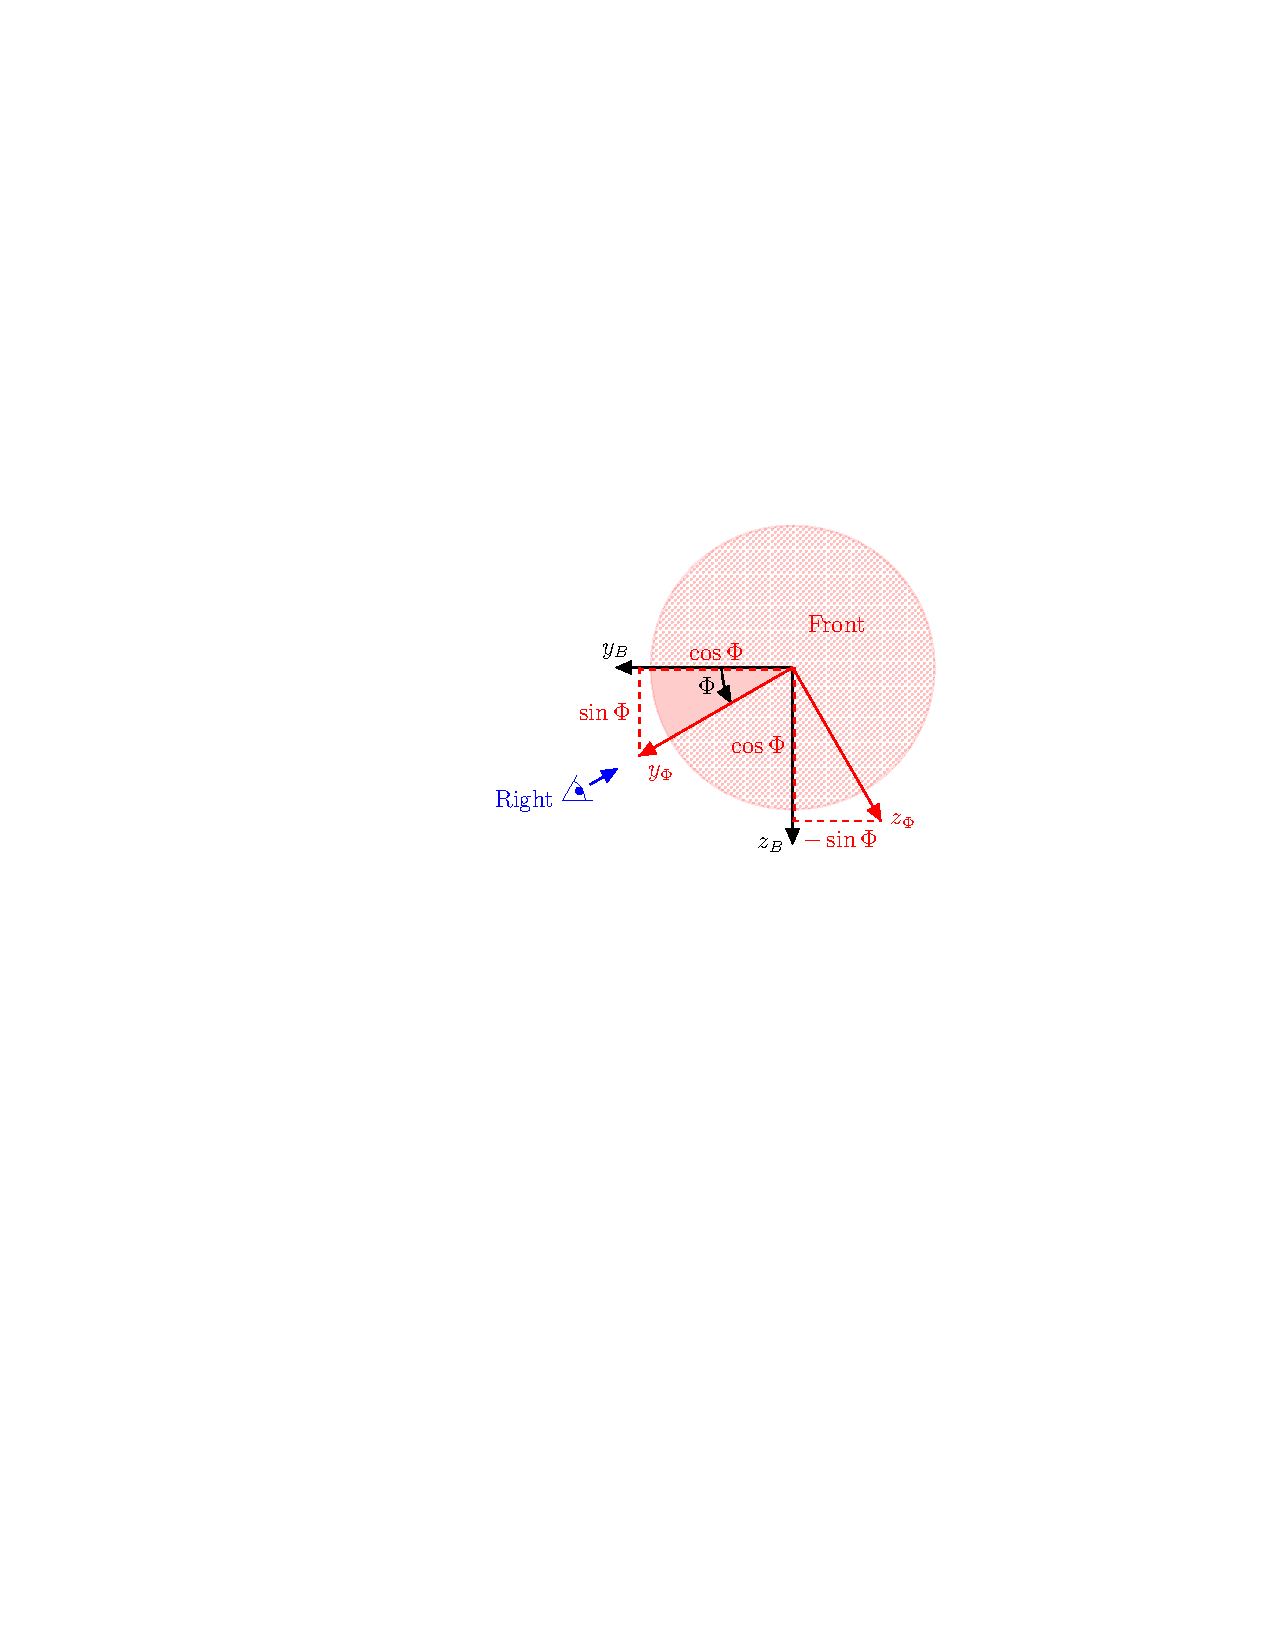
\includegraphics[clip=true, viewport=2.75in 4.875in 6.5in 7.5in,scale=.8]{figs/fig_dcm_2D_1.pdf}}\\
%  \vspace{-.25in} 
%  \subfloat[Pitch Rotation]{\label{fig: dcm_2D_2}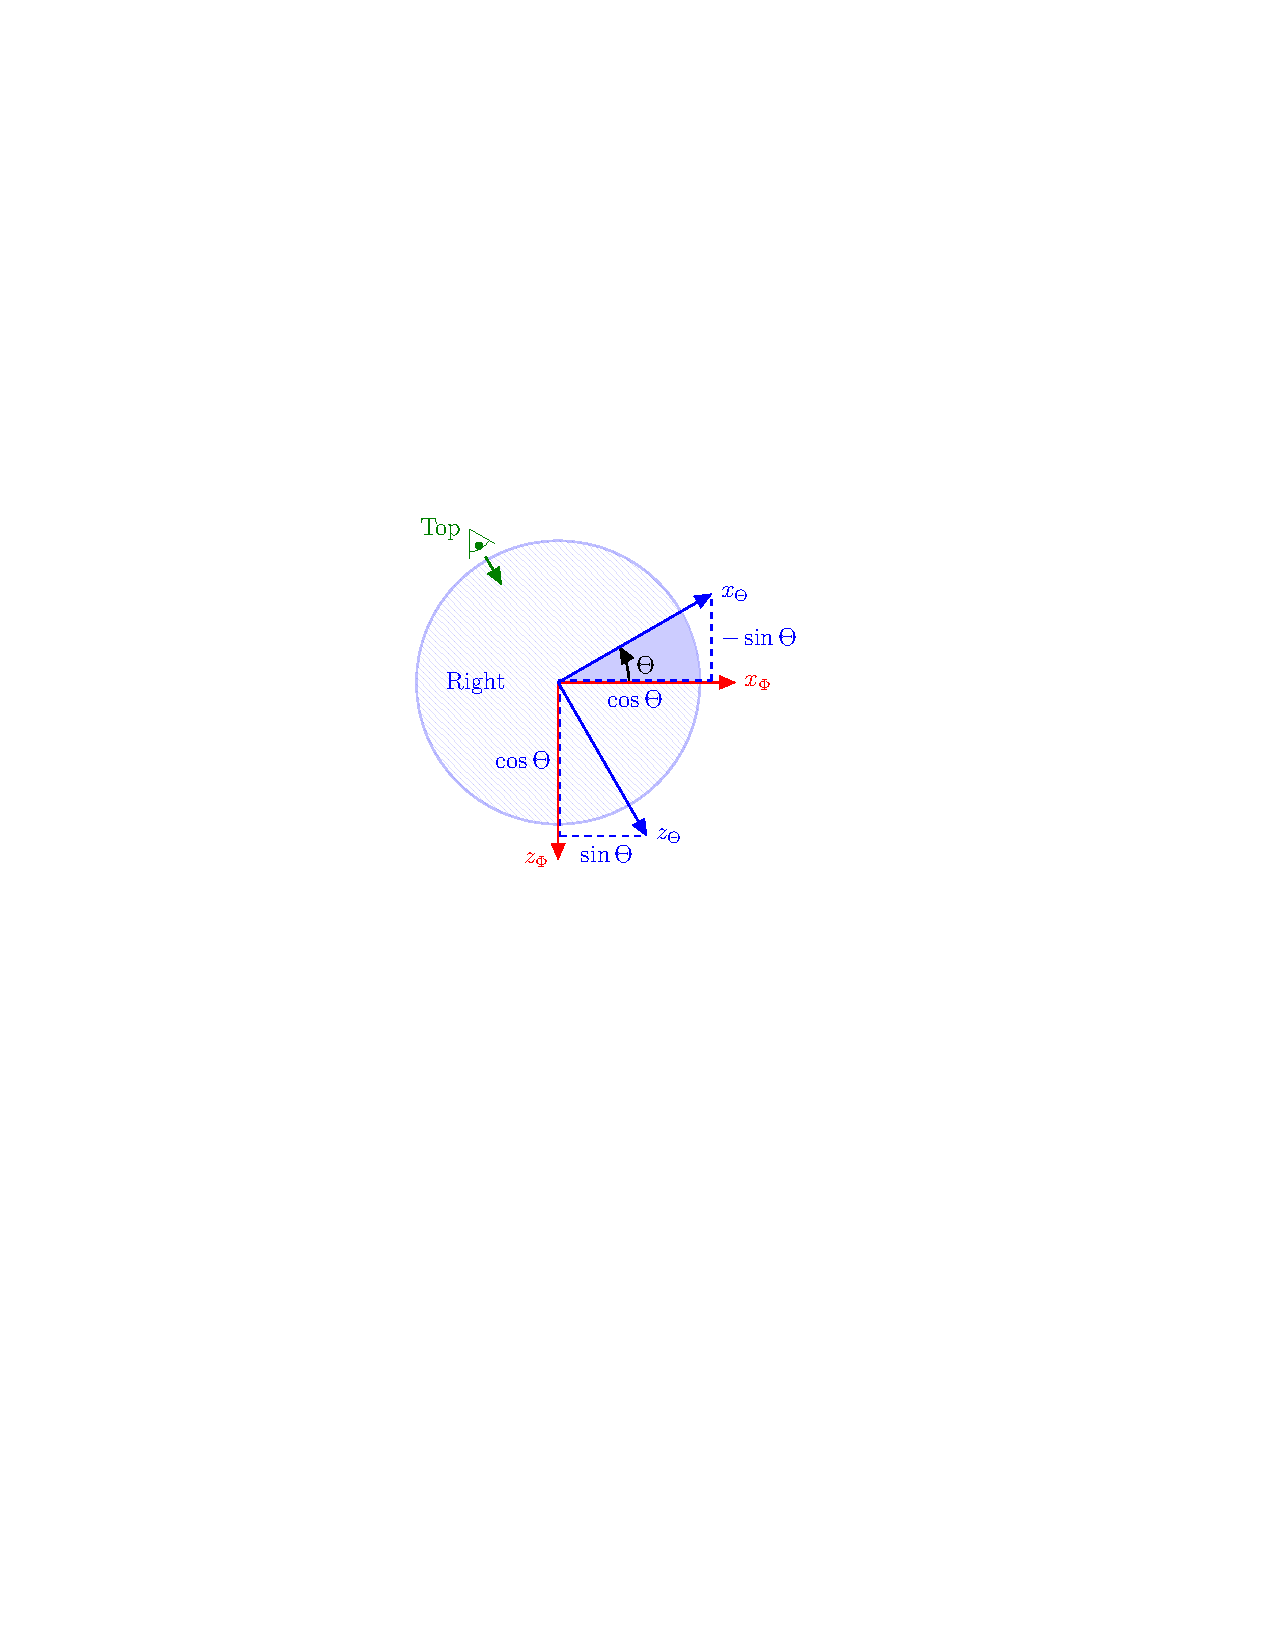
\includegraphics[clip=true, viewport=2.75in 4.875in 5.5in 7.75in,scale=.8]{figs/fig_dcm_2D_2.pdf}}\\
%  \subfloat[Yaw Rotation]{\label{fig: dcm_2D_3}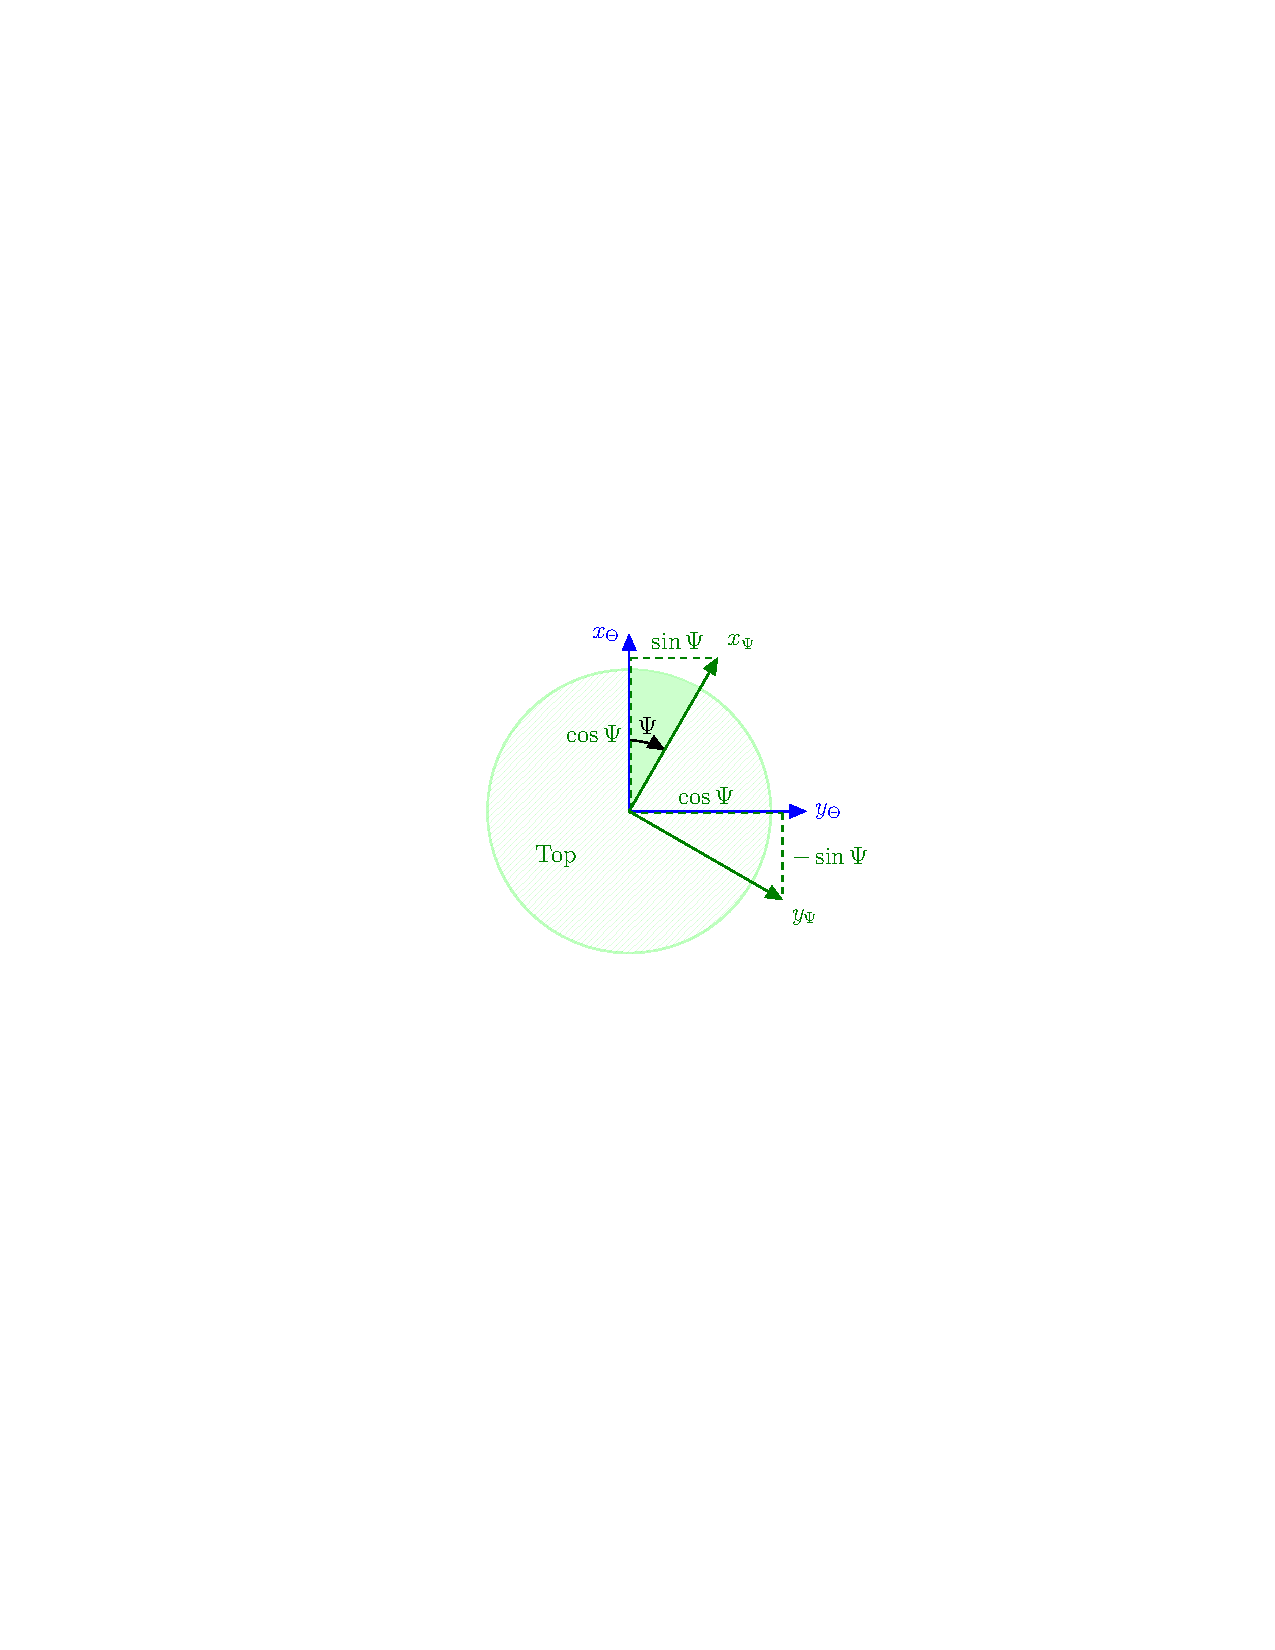
\includegraphics[clip=true, viewport=2.75in 4.5in 5.6in 7in,scale=.8]{figs/fig_dcm_2D_3.pdf}}%
%  \caption{Direction Cosine Matrix Projected Rotations}%
%  \label{fig: dcm_2D}%
%\end{wrapfigure}

As an example, the array $C_{\Phi}$ from \autoref{tab: dcm_plane_rot} may be read either left to right or down as $\vect{y_{\Phi}} = \vect{x_B}\;0 + \vect{y_B}\;\cos\Phi + \vect{z_B}\;\sin\Phi$ and $\vect{y_B} = \vect{x_{\Phi}}\;0 + \vect{y_{\Phi}}\;\cos\Phi - \vect{z_{\Phi}}\;\sin\Phi$ respectively. The transpose of $C_{\Phi}$, ie. $C_{\Phi}^{T}$ allows us to get to $\vect{x_{\Phi}}$, $\vect{y_{\Phi}}$, $\vect{z_{\Phi}}$ from $\vect{x}$, $\vect{y}$, $\vect{z}$, to be proven later. Doing the left to right read for the remaining rows and corresponding columns leads to a convenient matrix formulation of these equations:

	\begin{equation}   %TODO: Bold Equal Sign
		\left[ \begin{array}{c} \vect{x_{\Phi}} \\ \vect{y_{\Phi}} \\ \vect{z_{\Phi}} \end{array} \right] =
		\left[ \begin{array}{ccc} 1 & 0 & 0 \\ 0 & \cos\Phi & \sin\Phi \\ 0 & -\sin\Phi & \;\;\;\cos\Phi \end{array} \right]
		\left[ \begin{array}{c} \vect{x_B} \\ \vect{y_B} \\ \vect{z_B} \end{array} \right] 
		\qquad\Longleftrightarrow\qquad
		\vect{F_{\Phi}} \boldsymbol{=} C_{\Phi} \vect{F_{B}}
		\label{eq: DCM_y}
	\end{equation}

In this formulation $C_{\Phi}$ gets us to $\vect{x_B}$, $\vect{y_B}$, $\vect{z_B}$ from $\vect{x_{\Phi}}$, $\vect{y_{\Phi}}$, $\vect{z_{\Phi}}$. A variety of notations exist for direction cosine matrices, Stevens would write $C_{\vect{F_{\Phi}}/\vect{F_{B}}}$ instead of $C_{\Phi}$ which explicitly expresses the coordinate frame transformation in the subscript, ie. from $\vect{F_{B}}$ to $\vect{F_{\Phi}}$. Less trivial than notation are the properties which these rotation matrices possess:

\noindent 1. \textit{Orthogonality} \\
\indent If we let $Q$ be square, $n \times n$, matrix and suppose $Q^{-1}=Q^T$ then $Q$ is orthogonal if and only if: 
	\begin{equation}
		QQ^T=Q^TQ=I
		\label{eq: DCM_orthogonality}
	\end{equation}
where $I$ is the identity matrix. This implies that the rotated vector length is unchanged. %Thm 1
Alternatively, an orthogonal matrix may be defined as a square matrix with entries whose rows and columns are perpendicular and of unit length, ie. orthogonal unit vectors or orthonormal vectors. %Thm 2

\noindent 2. \textit{Non-Commutative} \\
\indent Direction cosine matrices do not commute:
	\begin{equation}
		C_1 C_2 \neq C_2 C_1
		\label{eq: DCM_non_commutative}
	\end{equation}

\noindent 3. \textit{Successive rotations may be described the by product of individual plane rotation matrices.} \\
\indent The orientation of a three-dimensional coordinate frame to another may be obtained by a sequence of three successive rotations. By tradition, aerospace applications perform these transformations through right handed rotations in each coordinate planes, referred to earlier as plane rotations, in the Z-Y-X order \citet{Stevens2003}; alternate sign convention and planes of rotation exist in other fields, eg. 3D modeling in computer science. Right handed rotation about the z-axis is positive yaw, right handed rotation about the y-axis is positive pitch, and right handed rotation about the x-axis is positive roll. Order of rotation sequence is arbitrary, \autoref{fig: DCM_RPY} depicts a complete coordinate transformation in a X-Y-Z (Roll-Pitch-Yaw) manner.
%
	\begin{figure}[htb]
		\centering
		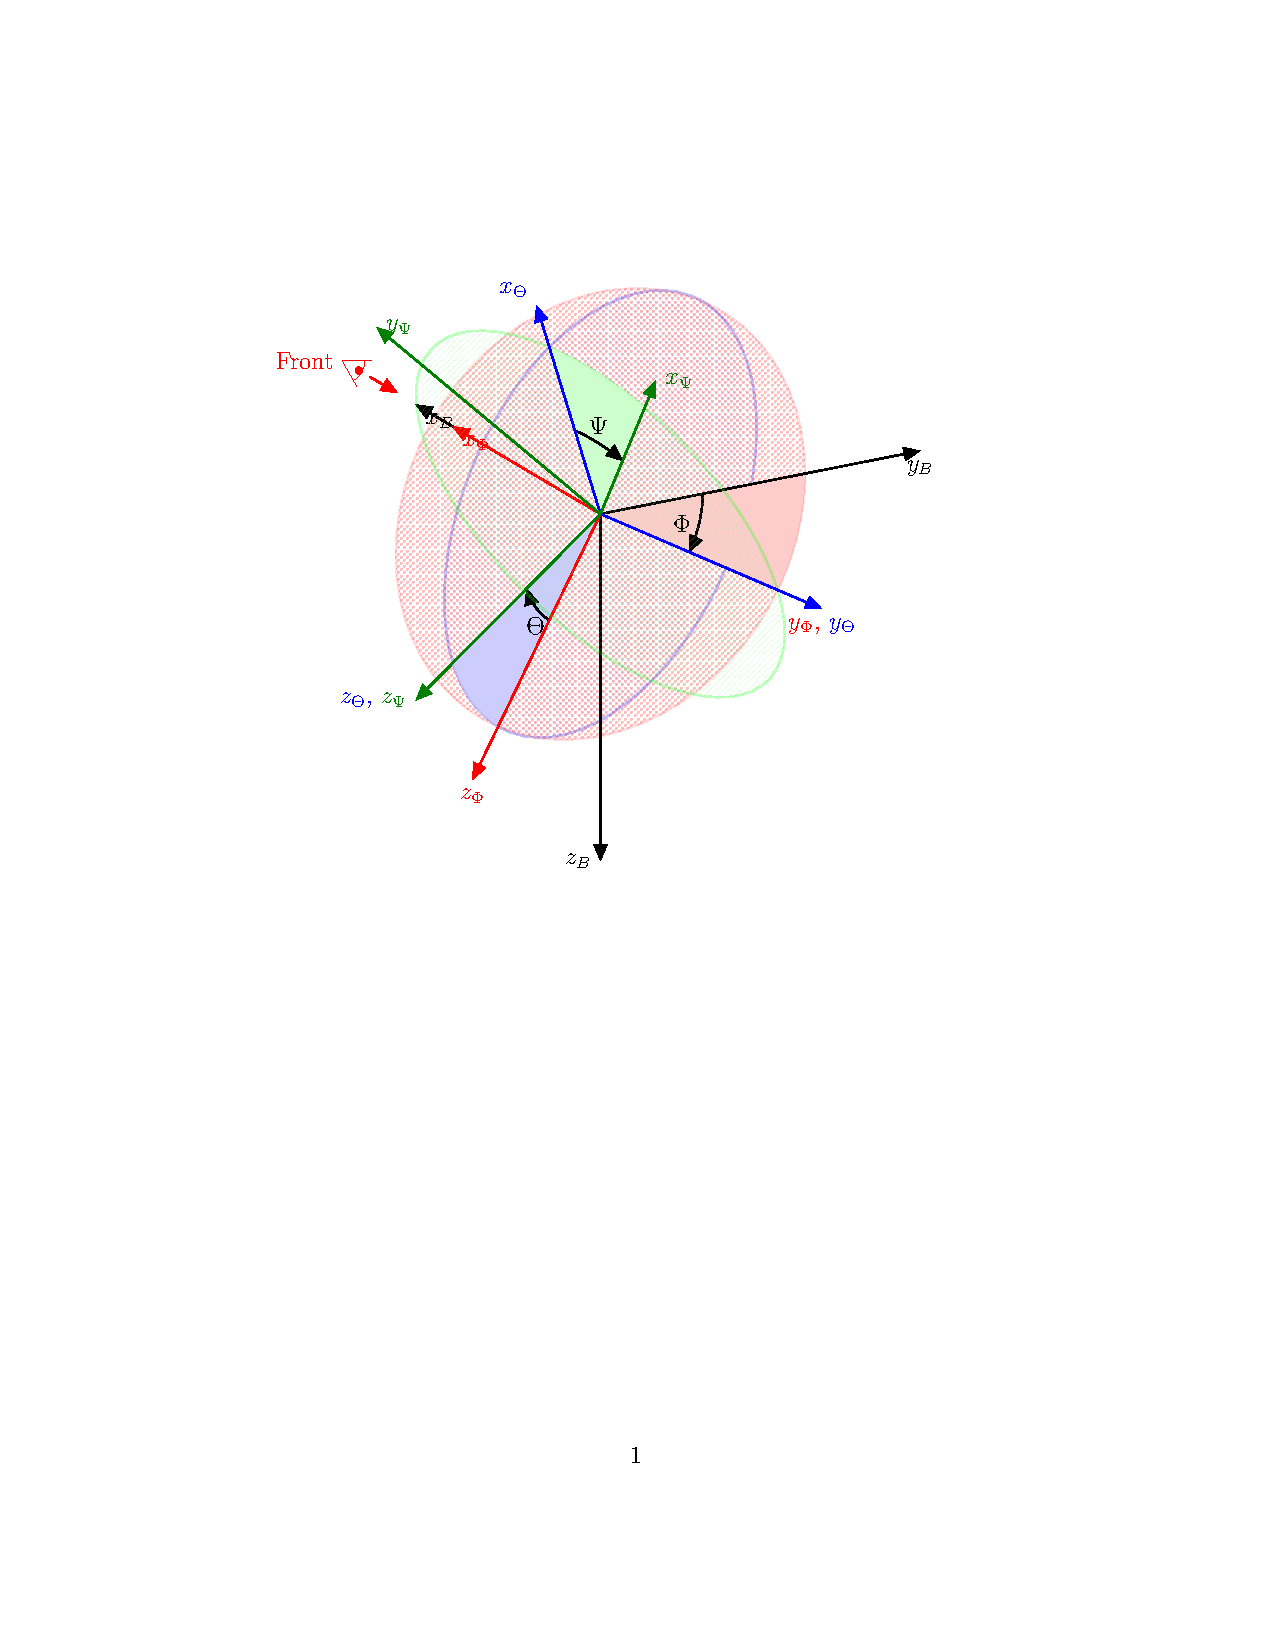
\includegraphics[clip=true, viewport=1in 5in 7in 9.25in,scale=.8]{figs/fig_dcm.pdf}%
		\caption{Direction Cosine Matrix Visual}%
		\label{fig: DCM_RPY}%
	\end{figure}
%
This rotation sequence is suitable for calculating aircraft attitudes with respect to the north-east-down frame. These angles of rotation are called \textbf{Euler angles}. In terms of coordinate transformations
%
	\begin{equation}
		\vect{F_{B}} = \left( C_{\Phi}C_{\Theta}C_{\Psi} \right) \, \vect{F_{NED}}
		\label{eq: DCM_NED_2_ABC}
	\end{equation}
%
where \autoref{eq: DCM_RPY} is the complete coordinate transformation from north-east-down to the body frame, ie. $C_{\vect{F_{NED}} / \vect{F_{B}}} = C_{\Phi}C_{\Theta}C_{\Psi} $
%
	\begin{equation}
		\resizebox{.9\hsize}{!}{$
		C_{\Phi}C_{\Theta}C_{\Psi} = \left[ \begin{array}{ccc}
		\cos\Theta \cos\Psi &  \cos\Theta \sin\Psi & -\sin\Theta  \\
		-\cos\Phi \sin\Psi  + \sin\Phi \sin\Theta \cos\Psi & \cos\Phi \cos\Psi + \sin\Phi \sin\Theta \sin\Psi &  \sin\Phi \cos\Theta  \\
		\sin\Phi \sin\Psi + \cos\Phi \sin\Theta \cos\Psi & -\sin\Phi \cos\Psi + \cos\Phi \sin\Theta \sin\Psi & \cos\Phi \cos\Theta \\
		\end{array} \right] $}
		\label{eq: DCM_RPY}
	\end{equation}

\subsection{Aircraft Dynamics}
\label{subsec: ac_dynamics}
%
With \manref{Assumptions}{ass: rigid} \& \ref{ass: inertial} in our front pocket, which is more accessible than the back pocket, we now have an idealized rigid body and live in a world suited for the application Newton's Laws. With this we can describe translational and rotational motion of the aircraft by its kinematic analogs: linear momentum, $\vect{p}$, and angular momentum, $\vect{H}$ respectively.

%Vehicle sensors are fixed and are therefore relative to the wind axis system. Translational equations are referenced to the wind axes and rotational equations are referenced to the body axes. This is convenient to the pilot who senses forces and acceleration relative to his position, however for navigation it is necessary to use axes relative to earth.
``By Newton's second law the time rate of change of linear momentum equals the sum of all \textit{externally} applied forces, [ $\vect{F}$ ].
%
	\begin{equation}
		\displaystyle \vect{F} = \frac{d}{dt}\left( \vect{p} \right) = \frac{d}{dt}\left( m \vect{V} \right)
		\label{eq: lin_mom}
	\end{equation}
%
\noindent and the rate of change of angular momentum is equal to the sum of all applied torques
%
	\begin{equation}
		\vect{M} = \frac{d}{dt} \left(\vect{H} \right)
		\label{eq: ang_mom}
	\end{equation}
%
These vector differential equations provide the starting point for a complete description of the rigid body motions of the vehicle.'' \citet{McRuer1973}
%
	\begin{ass}
		Mass is considered constant
		\label{ass: mass}
	\end{ass}
%
\noindent In most aerospace systems thrust is generated by an expenditure of vehicle mass; an exception being electric powered applications. Whether that trade in mass directly contributes to linear momentum or not needs to be considered. In the present propulsion case a heavy fuel piston engine turns a propeller, therefore the thrust generated may be considered an external force. Alternatively, if a jet engine were used there would be a component of thrust due to expulsion of vehicle mass\footnote{\citet{McRuer1973} derives a modified extension of \autoref{eq: lin_mom} to take this into account.}. 
%
%Applying assumption \ref{ass: mass} and expanding \autoref{eq: lin_mom} leads to the following three scalar equations which describe the motion of the airframe center of mass.
%%
%\begin{align}
%m \frac{d}{dt}\left( u \right) =& F_x \\
%m \frac{d}{dt}\left( v \right) =& F_y \\
%m \frac{d}{dt}\left( w \right) =& F_z 
%\label{eq: lin_mom_exp}
%\end{align}
%
%The rotary equivalent of linear momentum, angular momentum $\vect{H}$, is more complicated. The rotary equivalent of mass is the moment of inertia, $\vect{I}_{3x3}$. The angular momentum is the vector dot product of moment of inertia with angular velocity.
%
%\begin{equation}\label{eq: AngMomEquiv}
%\vect{H} = \vect{I}_{3x3} \cdot \Omega
%\end{equation}
%TODO: Rectilinear acceleration eg, to get to expanded forms of \autoref{eq: lin_mom} and \autoref{eq: ang_mom} introduced in beginning of next two sections?

\subsubsection{Translational Acceleration} $\,$
\label{subsubsec: trans}
%
The goal is to derive equations for translation accelerations in the wind axis reference frame, eventually arriving at $\dot{V}$, $\dot{\alpha}$, and $\dot{\beta}$. Picking up where \autoref{eq: lin_mom} left off, along with \manref{Assumption}{ass: mass}, we may expand the expression to
%
	\begin{equation}
		\vect{F} = m \left[ \frac{d}{dt} \left( \vect{V} \right) + \vect{\Omega} \times \vect{V} \right]
		\label{eq: lin_mom_nasa}
	\end{equation}%
%
where $\vect{F}$ is the total force acing on the vehicle, $m$ is the vehicle mass, $\vect{V}$ is the total vehicle velocity, and $\vect{\Omega}$ is the total vehicle angular velocity:
%
	\begin{equation}
		\vect{F} 		= \textstyle \left[ \begin{array}{c} \sum F_{x} \\ \sum F_{y} \\ \sum F_{z} \end{array}\right]= \left[ \begin{array}{c} 
		F_{x_{T}} + F_{x_{A}} + F_{x_{G}}\\
		F_{y_{T}} + F_{y_{A}} + F_{y_{G}}\\
		F_{z_{T}} + F_{z_{A}} + F_{z_{G}}
		\end{array}\right]
		\label{eq: lin_mom_F}
	\end{equation}%
	\nomenclature[B]{$T$}{Thrust}% % %  N O M E N C L A T U R E  % % %
	\nomenclature[B]{$A$}{Aerodynamic}% % %  N O M E N C L A T U R E  % % %
	\nomenclature[B]{$G$}{Gravitational}% % %  N O M E N C L A T U R E  % % %
%
	\begin{gather} %TODO: Figure out what velocity vector should relaly be...
		%\vect{V} 		= \left[\,V\cos\chi\cos\gamma,\,V\sin\chi\cos\gamma,\,-V\sin\gamma\,\right]^T \label{eq: lin_mom_V} \\
		\vect{V} 		= \left[\,u,\,v,\,w\,\right]^T \label{eq: lin_mom_V} \\
		\vect{\Omega} 	= \left[\,P,\,Q,\,R\,\right]^T \label{eq: lin_mom_O}
	\end{gather}
%
The elements of $\vect{F}$ are summations of externally applied propulsive (T), aerodynamic (A), and gravitational (G) forces respective to each body axis. It will be assumed that the engine is mounted to align with body axes, therefore there are no thrust-angles or $F_{y_{T}} = F_{z_{T}} = 0$. 

The body axis aerodynamic forces can be transformed to their equivalent stability axis components lift L, drag D, and side-force Y as \autoref{fig: vehicle_axes} indicates.
%
	\begin{figure}[H] 
		\centering
		\includegraphics[scale=1]{3_theory/vehicle_axes.png}
		\caption{Body Axes, Forces, and Moments}
		\label{fig: vehicle_axes}
	\end{figure}

	%TODO: Aerodynamic FBD - APPLY AOA
	\begin{align}
		F_{x_{A}} =& -D\cos\alpha + L\sin\alpha \\
		F_{y_{A}} =& \quad\, Y  \\
		F_{z_{A}} =& -D\sin\alpha - L\cos\alpha
	\end{align}%

The gravitational forces can be resolved into body axis components such that

	%TODO: Gravity FBD
	\begin{figure}[H] 
		\centering
		\includegraphics[scale=.5]{3_theory/EOM/grav.png}
		\caption{Orientation of Gravity Vector with Respect to Body Axes \citep{McRuer1973}}
		\label{fig: grav}
	\end{figure}
	%
	\begin{align}
		F_{x_{G}} =& -mg\sin\theta \\
		F_{y_{G}} =& \quad\, mg\sin\phi\cos\theta \\
		F_{z_{G}} =& \quad\, mg\cos\phi\cos\theta
	\end{align}

Combining these we arrive at an expression that considers all external forces acting on the airframe.
%
	\begin{equation}
		\left[ \begin{array}{c} \sum F_{x} \\ \sum F_{y} \\ \sum F_{z} \end{array}\right] = \left[ \begin{array}{c} 
		F_{x_{T}} - D\cos\alpha + L\sin\alpha - mg\sin\theta \\
		Y + mg\sin\phi\cos\theta\\
		-D\sin\alpha - L\cos\alpha + mg\cos\phi\cos\theta
		\end{array}\right]
		\label{eq: lin_mom_F_sub}
	\end{equation}

By rearranging \autoref{eq: lin_mom_nasa} to solve for translational acceleration, $d\vect{V}/dt$, we can express body axis accelerations in terms of body axis forces, angular rates, and velocities: 
%
	\begin{equation}
		\frac{d}{dt} \left( \vect{V} \right) = \frac{1}{m} \vect{F}- \vect{\Omega} \times \vect{V}
		\label{eq: lin_mom_nasa_re}
	\end{equation}%

Substitution of \manref{Equations}{eq: lin_mom_V}, \ref{eq: lin_mom_O}, and \ref{eq: lin_mom_F} yields 
%
	\begin{equation}
		\left[ \begin{array}{c} \dot{u} \\ \dot{v} \\ \dot{w} \end{array}\right] = \left[ \begin{array}{c} \frac{1}{m} \left(
		F_{x_{T}} + F_{x_{A}} + F_{x_{G}} \right) + Rv - Qw\\
		\frac{1}{m} \left(F_{y_{T}} + F_{y_{A}} + F_{y_{G}} \right) + Pw - Ru \\
		\frac{1}{m} \left(F_{z_{T}} + F_{z_{A}} + F_{z_{G}} \right) + Qu - Pv
		\end{array}\right]
		\label{eq: uvw_dot}
	\end{equation}

In order to express \manref{Equation}{eq: uvw_dot} in the wind axis system, $[\dot{V}$, $\dot{\alpha}$, $\dot{\beta}]^T$ , will need to use the aforementioned equations
	\begin{align}
		u	=& V\cos\beta\cos\alpha 	\tag{\ref{eq: body_u}} \\
		v	=& V\sin\beta 				\tag{\ref{eq: body_v}} \\
		w	=& V\cos\beta\sin\alpha 	\tag{\ref{eq: body_w}}
	\end{align}
%
	and transforms
	\begin{align}
		V		=& \sqrt{u^{2}+v^{2}+w^{2}} \tag{\ref{eq: wind_v}} \\
		\alpha 	=& \tan^{-1}\left( \displaystyle \frac{w}{u} \right) \tag{\ref{eq: wind_alpha}} \\
		\beta	=& \sin^{-1} \left( \displaystyle \frac{v}{\sqrt{u^{2}+v^{2}+w^{2}}} \right) \tag{\ref{eq: wind_beta}}
	\end{align}
%
Refer to \citet[Appendix B.]{Duke1988} to see the remainder of the derivation, ie. how to take derivatives and make the appropriate substitutions to arrive at $\dot{V}$, $\dot{\alpha}$, and $\dot{\beta}$ equations:
	\begin{align*}
		\dot{V} 	\quad=\quad&  \frac{1}{m}\left(- D\cos\beta + Y\sin\beta + T\cos\alpha\cos\beta \right) - g\sin\gamma \\
		\dot{\alpha}\quad=\quad& -\frac{1}{mV\cos\beta}\left(L + T\sin\alpha \right) + \frac{g\cos\gamma\cos\mu}{V\cos\beta} + Q  - \tan\beta\left(P\cos\alpha + R\sin\alpha\right) \\
		\dot{\beta} \quad=\quad&  \frac{1}{mV}\left(D\sin\beta + Y\cos\beta - T\sin\beta\cos\alpha \right) + \frac{g\cos\gamma\sin\mu}{V} + P\sin\alpha - R\cos\alpha
	\end{align*}
%
\subsubsection{Rotational Acceleration}
\label{subsubsec: rot}
%
The goal is to derive rotational acceleration equations -- $\dot{P}$, $\dot{Q}$, $\dot{R}$. Picking up where \autoref{eq: ang_mom} left off and substituting total angular momentum for the product of the moment of inertia matrix and rotational velocity vector, $\vect{H} = \vect{I}\vect{\Omega}$, we may expand the expression to
%
	\begin{equation}
		\vect{M} = \left[ \frac{d}{dt} \left( \vect{I}\vect{\Omega} \right) + \vect{\Omega} \times \vect{I}\vect{\Omega} \right]
		\label{eq: ang_mom_nasa}
	\end{equation}
%
where $\vect{M}$ is the total moment acing on the vehicle, $\vect{I}$ is the inertia matrix (alternatively referred to as tensor or dyad), and $\vect{\Omega} = [P,\,Q,\,R]^T$ is the total vehicle angular velocity:
	\begin{equation}
		\vect{M} = \textstyle \left[ \begin{array}{c} \sum \bar{L} \\ \sum \bar{M} \\ \sum \bar{N} \end{array}\right]= \left[ \begin{array}{c} 
		\bar{L} + \bar{L}_T \\
		\bar{M} + \bar{M}_T \\
		\bar{N} + \bar{N}_T 
		\end{array}\right]
		\label{eq: ang_mom_L}
	\end{equation}
%
\indent $\bar{L}$, $\bar{M}$ ,and $\bar{N}$ are the total aerodynamic moments about the $x_B$, $y_B$, and $z_B$ body axes with T subscript indicates moments induced by the power-plant.
%
	\begin{equation}    %http://ocw.mit.edu/courses/aeronautics-and-astronautics/16-07-dynamics-fall-2009/lecture-notes/MIT16_07F09_Lec26.pdf
		\vect{I} = \left[\begin{array}{ccc} 
							\,\; I_{xx} & - I_{xy} & - I_{xz} \\
							- I_{xy} & \,\; I_{yy} & - I_{yz} \\
							- I_{xz} & - I_{yz} &  \,\; I_{zz}
						 \end{array}\right]
		\label{eq: ang_mom_I}
	\end{equation}
	\nomenclature[+]{$I$}{Moment or Product of Inertia \nomunit{$\mathrm{slug \cdot ft^2}$}}% % %  N O M E N C L A T U R E  % % %
%
\indent Elements along the main diagonal are called the \textbf{moments of inertia} with respect to the x, y, and z axes respectively and are always positive. The off diagonal terms are referred to as the \textbf{products of inertia} and may be positive, negative, or zero; they are measures of the imbalance in mass distribution. Note that it is possible to orient the axes in such a way that the products of inertia are zero. In this case the diagonal terms are called the principal moments of inertia. 

	\begin{ass}
	The XZ plane is a plane of symmetry.
	\label{ass: sym}
	\end{ass}

\noindent This is a very good approximation for most air vehicles, and leads to $I_{yz} = 0$ as well as $I_{xy} = 0$. If we assume that the inertia tensor is constant, as we did with mass in the translational acceleration derivation, then \autoref{eq: ang_mom_nasa} may be rewritten as
%
	\begin{equation}
		\frac{d}{dt} \vect{\Omega} = \vect{I}^{-1} \left( \vect{M} - \vect{\Omega} \times \vect{I}\vect{\Omega} \right)
		\label{eq: ang_mom_nasa_re}
	\end{equation}
%
where $ d\vect{\Omega}/dt  = \left[ \, \dot{P}, \, \dot{Q}, \, \dot{R} \, \right]^T$.
%
%\begin{equation}
%	\vect{I}^{-1} = \frac{1}{\text{det}I} \left[ \begin{array}{ccc} 
%	I_{1} & I_{2} & I_{3} \\
%	I_{4} & I_{5} & I_{6} \\
%	I_{7} & I_{8} & I_{9}
%	\end{array} \right]
%	\label{eq: ang_mom_Iinv}
%\end{equation}
%
Refer to \citet[Sec. 1.2.1]{Duke1988} to see the remainder of the derivation, ie. how to make the appropriate substitutions to arrive at $\dot{P}$, $\dot{Q}$, and $\dot{R}$ equations. This is further simplified by \citet[Pg. 80]{Stevens1992}:
%
	\begin{align*}
		\dot{P} \quad=\quad& 	\left(c_1 R + c_2 P \right)Q + c_3 \bar{L} + c_4 \bar{N} \\
		\dot{Q} \quad=\quad& 	c_5 PR - c_6 \left( P^2 - R^2\right) + c_7 \bar{M} \\
		\dot{R} \quad=\quad& 	\left( c_8 P - c_2 R \right) Q + c_4 \bar{L} + c_9 \bar{N}
	\end{align*}
where \citep{Stevens1992} defines $c$ terms as

	\begin{equation} \label{eq: stevens_c}
		\begin{aligned}
			\Gamma     \quad=\quad	& I_{xx} I_{zz} - I_{xz}^2 \qquad \qquad & c_5 \quad=\quad 	& \frac{I_{zz} - I_{xx}}{I_{yy}}\\
			\Gamma c_1 \quad=\quad 	& \left( I_{yy} - I_{zz} \right) I_{zz} - I_{xz}^2 \qquad \qquad & c_6 \quad=\quad 	& \frac{I_{xz}}{I_{yy}}\\
			\Gamma c_2 \quad=\quad 	& \left( I_{yy} - I_{zz}\right) I_{zz} - I_{xz}^2 \qquad \qquad & c_7 \quad=\quad 	& \frac{1}{I_{yy}}\\
			\Gamma c_3 \quad=\quad 	& I_{zz} \qquad \qquad & \Gamma c_8 \quad=\quad 	& I_{xx}\left(I_{xx} - I_{yy}\right) + I_{xz}^2\\
			\Gamma c_4 \quad=\quad 	& I_{xz} \qquad \qquad & \Gamma c_9 \quad=\quad 	& I_{xx}\\
		\end{aligned}
	\end{equation}
%
\subsubsection{Attitude Rates}
\label{subsubsec: att}
%
Attitudes $\dot{\chi}$, $\dot{\gamma}$, and $\dot{\mu}$ may be derived by observing the velocity of the wind-axis system with respect to the gravity vector. Derivations in an Euler sense ($\phi,\,\theta,\,\psi$) are shown in \citet[Pg. 222]{McRuer1973} and \citet[Sec. 1.2.3]{Duke1988}. Similarly to the wind-axis attitude derivation, the flight-path components end up being:

\begin{align*}
	\dot{\chi} \quad=\quad	& \frac{1}{mV\cos\gamma}\left[ D\sin\beta\cos\mu + Y\cos\beta\cos\mu + L\sin\mu \right.\\
	 												& +\left. T\left(\sin\alpha\sin\mu - \cos\alpha\sin\beta\cos\mu \right) \right] \\
	\dot{\gamma} \quad=\quad& \frac{1}{mV}\left[-D\sin\beta\sin\mu - Y\cos\beta\sin\mu + L\cos\mu \right.\\
														& +\left. T\left(\sin\alpha\cos\mu + \cos\alpha\sin\beta\sin\mu\right)\right] - \frac{g}{V}\cos\gamma \\
	\dot{\mu} \quad=\quad	& \frac{1}{mV}\left[D\sin\beta\tan\gamma\cos\mu + Y\cos\beta\tan\gamma\cos\mu + L\left(\tan\beta + \tan\gamma\sin\mu\right) \right.  \\
													& +\left. T\left(\sin\alpha\tan\gamma\sin\mu + \sin\alpha\tan\beta - \cos\alpha\sin\beta\tan\gamma\cos\mu\right)\right] \\
													& -\frac{g\tan\beta\cos\gamma\cos\mu}{V} + \frac{P\cos\alpha + R\sin\alpha}{\cos\beta}  \\
\end{align*}
%
\begin{figure}[H]%
	\centering%
	\includegraphics[scale=1]{fury-1500-2.jpg}%
	\caption{Fury 1500 UAS on Launcher [\href{http://www.aviationweek.com/aw/blogs/defense/index.jsp?plckController=Blog\&plckBlogPage=BlogViewPost\&newspaperUserId=27ec4a53-dcc8-42d0-bd3a-01329aef79a7\&plckPostId=Blog\%3a27ec4a53-dcc8-42d0-bd3a-01329aef79a7Post\%3ad7b30f2c-a25b-4f47-90e5-46ff5606094c\&plckScript=blogScript\&plckElementId=blogDest}{www.aviationweek.com/aw/blogsmain/}]}%
	\label{fig: fury_1500_2}%
\end{figure}%

\subsubsection{Equations of Motion}
\label{subsubsec: eom}
Collecting equations from the previous sections, the complete set of nonlinear equations of motion turn out to be
\begin{subequations} \label{eq: eom}
	\begin{align}
	\label{eq: eom_chidot}  	\dot{\chi} \quad=\quad	& \frac{1}{mV\cos\gamma}\left[ D\sin\beta\cos\mu + Y\cos\beta\cos\mu + L\sin\mu \right.\\
	 												& +\left. T\left(\sin\alpha\sin\mu - \cos\alpha\sin\beta\cos\mu \right) \right] \nonumber \\
	\label{eq: eom_gamdot}  	\dot{\gamma} \quad=\quad& \frac{1}{mV}\left[-D\sin\beta\sin\mu - Y\cos\beta\sin\mu + L\cos\mu \right.\\
													& +\left. T\left(\sin\alpha\cos\mu + \cos\alpha\sin\beta\sin\mu\right)\right] - \frac{g}{V}\cos\gamma \nonumber \\
	\label{eq: eom_vdot}  	\dot{V} \quad=\quad		& \frac{1}{m}\left(- D\cos\beta + Y\sin\beta + T\cos\alpha\cos\beta \right) - g\sin\gamma \\
	\nonumber \\
	\label{eq: eom_mudot}  	\dot{\mu} \quad=\quad	& \frac{1}{mV}\left[D\sin\beta\tan\gamma\cos\mu + Y\cos\beta\tan\gamma\cos\mu + L\left(\tan\beta + \tan\gamma\sin\mu\right) \right. \nonumber \\
													& +\left. T\left(\sin\alpha\tan\gamma\sin\mu + \sin\alpha\tan\beta - \cos\alpha\sin\beta\tan\gamma\cos\mu\right)\right] \\
													& -\frac{g\tan\beta\cos\gamma\cos\mu}{V} + \frac{P\cos\alpha + R\sin\alpha}{\cos\beta} \nonumber \\
	\label{eq: eom_alphdot} 	\dot{\alpha} \quad=\quad& -\frac{1}{mV\cos\beta}\left(L + T\sin\alpha \right) + \frac{g\cos\gamma\cos\mu}{V\cos\beta} + Q \\
													& - \tan\beta\left(P\cos\alpha + R\sin\alpha\right) \nonumber \\
	\label{eq: eom_betadot} 	\dot{\beta} \quad=\quad	& \frac{1}{mV}\left(D\sin\beta + Y\cos\beta - T\sin\beta\cos\alpha \right) + \frac{g\cos\gamma\sin\mu}{V} \\
													& + P\sin\alpha - R\cos\alpha  \nonumber \\
	\nonumber \\
	\label{eq: eom_pdot} 	\dot{P} \quad=\quad		& \left(c_1 R + c_2 P \right)Q + c_3 \bar{L} + c_4 \bar{N} \\
	\label{eq: eom_qdot} 	\dot{Q} \quad=\quad		& c_5 PR - c_6 \left( P^2 - R^2\right) + c_7 \bar{M} \\
	\label{eq: eom_rdot} 	\dot{R} \quad=\quad		& \left( c_8 P - c_2 R \right) Q + c_4 \bar{L} + c_9 \bar{N}
	\end{align}
\end{subequations}
\nomenclature[+]{$D$}{Drag \nomunit{$\mathrm{lb_f}$}}			%% % %  N O M E N C L A T U R E  % % %
\nomenclature[+]{$Y$}{Sideforce \nomunit{$\mathrm{lb_f}$}}		% % %  N O M E N C L A T U R E  % % %
\nomenclature[+]{$L$}{Lift \nomunit{$\mathrm{lb_f}$}}			% % %  N O M E N C L A T U R E  % % %
\nomenclature[+]{$\bar{L}$, $\bar{M}$, $\bar{N}$}{Roll, Pitch, and Yaw Moments \nomunit{$\mathrm{lb \cdot ft}$}}% % %  N O M E N C L A T U R E  % % %
\nomenclature[-]{$m$}{Mass \nomunit{slug}}						% % %  N O M E N C L A T U R E  % % %
where $c$ terms are defined in \autoref{eq: stevens_c}.

\subsection{System Observations}
\label{subsec: system_observations}
The nonlinear differential equations summarized in \manref{Sec.}{subsubsec: eom} may be reduced to the form%
%
\begin{equation}
	\dot{\vect{x}} = \vect{f} \left( \vect{x},t \right)
	\label{eq: x_dot}
\end{equation} %$\vect{x} \in \mathbb{R}^n$ and $\vect{f}: \mathbb{R}^n \rightarrow \mathbb{R}^n$
%
where $\dot{\vect{x}}$ is the $n\times 1$ derivative of the state vector with respect to time, $\vect{f}$ is an $n\times 1$ nonlinear vector function expressing the six-degree of freedom rigid body equations, and $\vect{x}$ is the $n\times 1$ state-vector with respect to time. Additionally, the state-vector is defined as a set of real numbers, ${(x_1,\ldots,x_n)}^T$, contained in $n$-dimensional Euclidean space, denoted by the symbol  $\mathbb{R}^n$, and is formally referred to as \textbf{state-space}. The parameter $n$ is the \textbf{system order}\footnote{The highest derivative of the dependent variable with respect to the independent variable appearing in the equation.} and refers to the number of first order differential equations required to represent an equivalent $n^{th}$ order ordinary differential equation (ODE).

\autoref{eq: x_dot} represents the closed-loop time-variant dynamics of a feedback control system, even though it does not explicitly contain a control input vector $\vect{u}$. This is because the control input may be considered a function of state $\vect{x}$ and time $t$, therefore \textit{disappearing} in the closed-loop dynamics. Showing this mathematically, if the plant dynamics are
%
\begin{equation}
	\dot{\vect{x}} = \vect{f} \left( \vect{x},\vect{u},t \right)
	\label{eq: x_dot_g}
\end{equation}
%
and some control law $\vect{u}$ has been selected as
\begin{equation}
	\vect{u} = \vect{g} \left( \vect{x},t \right)
	\label{eq: x_dot_u}
\end{equation}
%
then the closed-loop dynamics are
\begin{equation}
	\dot{\vect{x}} = \vect{f} \left[ \vect{x},\vect{g} \left( \vect{x},t \right),t \right]
	\label{eq: x_dot_g_u}
\end{equation}
%
which can be rewritten in the form of \autoref{eq: x_dot}; since $\vect{g}(\vect{x},t)$ is a function of the state $\vect{x}$, which is already represented in the expression, it may be discarded. Naturally, \autoref{eq: x_dot} may also represent a system without control input, such as a freely moving spring-mass damper or pendulum. These examples, as with all physical systems, are time dependent.

Given a particular initial condition, an ODE may have several system trajectories. Continuity of $\vect{f}$, ie.
$\displaystyle \lim_{x \rightarrow a}\vect{f}(x)=\vect{f}(a)$, ensures that there is at least one solution but does not ensure uniqueness of the solution. A stronger and therefore more frequently used condition, that guarantees \textit{Lipschitz} continuity, may be used to prove existence \textit{and} uniqueness as well as protect against the possibility of $\vect{f}(x)$ having an infinite slope, eg. a discontinuity.

\begin{defn}[Lipschitz Condition] \alignright \citet[\S 2.2]{Khalil1996}\\
	If there exists a strictly positive Lipschitz constant $L$ such that $\vect{f}(\vect{x},t)$ satisfies the inequality,
	$$ \lVert \vect{f}(\vect{x},t) - \vect{f}(\vect{y},t) \rVert \leq L \lVert \vect{x} - \vect{y} \rVert \qquad \forall \, \vect{x}, \vect{y} \in \mathcal{D}$$
	then the function $\vect{f}(\vect{x},t)$ is said to be \textit{Lipschitz in} $\vect{x}$ for all points in the domain $\mathcal{D}$. 
	\label{defn: lipschitz}
\end{defn}

Further specifying conditions on the domain $\mathcal{D}$, over which the Lipschitz condition holds, imposes restrictions on input values for the function $\vect{f}(\vect{x},t)$. A function is said to be \textit{locally Lipschitz in} $\vect{x}$ if that for each point $\vect{x} \in \mathcal{D} \subset \mathbb{R}^n$ there exists a finite neighborhood $\mathcal{D}_0 \in \mathcal{D}$ such that the Lipschitz condition holds for all points in $\mathcal{D}_0$ with a corresponding Lipschitz constant $L_0$.

\begin{thm}[Global Existence and Uniqueness] \alignright \citet[Thm 2.4]{Khalil1996}\\
	Let $\vect{f}(\vect{x},t)$ be piecewise continuous in $t$ and \textbf{locally Lipschitz in} $\vect{x}$ for all $t \geq t_0$ and all $\vect{x}$ in a domain $D \subset \mathbb{R}^n$ and let W be a \textbf{compact (closed and bounded) subset} of $\mathcal{D}$. If for $x_0 \subset W$ it is known that every solution of
	$$ \dot{\vect{x}} = \vect{f}(\vect{x},t), \quad \vect{x}(t_0) = \vect{x_0} \qquad \forall t \geq t_0$$
	lies entirely in W. Then there is a \textbf{unique solution} that is defined for all $t \geq t_0$
	\label{thm: lipschitz}
\end{thm}

\begin{proof}[]
	Refer to \citet[Pg. 77]{Khalil1996}
\end{proof}

``The trick in applying \manref{Theorem}{thm: lipschitz} is in checking the assumption that every solution lies in a compact set without actually solving the differential equation.'' This concept is introduced in Lyapunov's stability definitions to come.

\begin{defn}[Autonomous and Non-Autonomous Systems] \alignright \citet{Slotine1991} \\
	The nonlinear system $\dot{\vect{x}} = \vect{f} \left( \vect{x},t \right)$ is said to be \textbf{autonomous} if $\vect{f}$ does not depend explicitly on time, ie. if the system's state equation can be written
	\begin{equation}
		\dot{\vect{x}} = \vect{f}(\vect{x})
		\label{eq: x_dot_auto}
	\end{equation}
	otherwise, the system is called \textbf{non-autonomous}. 
	\label{defn: auto}
\end{defn}
%
Again, all real-world systems are non-autonomous, but ``in practice system properties often change very slowly, so we can neglect their time variation without causing any practically meaningful error.''\citep{Slotine1991} Most importantly, \manref{Definition}{defn: auto} implies that solutions, or system trajectories, of autonomous ODEs are independent of initial time, thereby greatly simplifying stability analysis; In other words, stability for autonomous systems does not depend on initial conditions.

\section{Stability}
\label{sec: stability}
%
The goal is to familiarize the reader with concepts required to prove stability for the backstepping control architecture. Most proofs will not be included, but will be referenced immediately succeeding theorems. It is assumed that the reader has a good understanding of solution properties to ordinary differential equations such as existence, uniqueness, and continuity. Mathematical notation and terminology tied to these properties may be used in subsequent theorems and definitions without introduction. A great overview of mathematical preliminaries pertinent to nonlinear systems and backstepping control is included in \citet[Chp. 2]{Khalil1996}. The following standard mathematical abbreviation symbols shall be used:
\begin{align*}
	\forall 	\quad & \quad \text{``for all''} 		\qquad & \qquad 	\in 		\quad & \quad \text{``in'' or ``belongs to''}	\\
	\exists 	\quad & \quad \text{``there exists''}	\qquad & \qquad		\subset		\quad & \quad \text{``a subset of''}			\\
	\ni 		\quad & \quad \text{``such that''}		\qquad & \qquad		\Rightarrow \quad & \quad \text{``implies''}
\end{align*}

Backstepping control designs are constructed using Lyapunov stability theory. This is currently the ``most useful and general approach,'' \citet{Slotine1991}, to establishing stability for nonlinear systems and may also be extended to linear systems. It was published in 1892 by Russian mathematician Alexandr Lyapunov in \textit{The General Problem of Motion Stability} \textit{for systems without inputs}. As a consequence it has traditionally been applied to closed-loop control systems, ie. those in which a feedback control law has already been selected. Later, in \manref{Sec.}{sub: lyapunov_based}, a method for designing a feedback control law in conjunction with Lyapunov theory will be introduced. Furthermore, Lyapunov stability theory provides two methods for stability analysis, indirect and direct. The first method\footnote{In my research I found conflicting evidence on what Lyapunov's first method actually was. \citep{Slotine1991} warns the reader that linearization is sometimes incorrectly referred to as the first method, which should be Lyapunov's method of exponents. This was confirmed, as many other sources I found on the topic referred to the indirect method as the first method.}, indirect or linearization, determines \textit{local} stability properties; eigenvalues of a linear (approximate, hence indirect) system reveals stability in the immediate vicinity of an equilibrium point. The second method, direct, determines \textit{regional} stability properties; the aim is to make the system act like a function whose time derivative guarantees some form of stability. Since our system equations are nonlinear only Lyapunov's direct method will be covered.

Ultimately, this section condenses the philosophy, definitions, and theorems of \citet[Chp. 3]{Slotine1991}, \citet[Chp. 3]{Khalil1996}, \citet[Chp. 3]{Harkegard2003}, \citet[Chp. 2]{Krstic95} and \citet[Appendix A]{Farrell2006} in a brief and clear manner.

%TODO: integrate classic stability or not...
%The traditional development of stability set by aircraft stability and control textbooks typically do not deal with nonlinear systems. Stability development for linear systems is traditionally\footnote{Most introductory aerospace controls books: Nelson, McRuer, P\&H, Etkin,... \color{red}\textbf{validate this claim}} derived from a classical mechanics perspective, where familiar terms like dynamic and static stability are used to respectfully characterize transient response and steady-state equilibrium due to small perturbations. 
%
%\textbf{Static Stability}
%
%Pg 99 Stevens 2003, Pg 55 Stevens 1992
%
%Steady state flight, forces and moments are constant in the body reference frame
%
%Ball and hill example, define stable vs. unstable and elaborate... reference Dr. Mehiel/Dr. K's lectures
%
%\textbf{Dynamic Stability}
%
%Pg 374/375 P\&H
%
%``In order to understand the requirements for static stability and control it is necessary to study the dynamic characteristics of the airplane.'' \citep{Perkins1949} We can define particular types of motion by examining the transient response due to a given disturbance -- a theoretical perturbation or one generated by the deflection of a control surface -- from an equilibrium flight condition. ``The characteristic modes of motion of the airplane must be known in order to determine the nature of the control required to fly the airplane. For example, if the emotion of the airplane in response to some disturbance was a very slow divergence, the control requirements would be completely different from those needed if the divergence was extremely rapid. The ability of the human pilot to react an apply the controls is a factor which must be kept well in mind during all studies of airplane dynamics.'' \citep{Perkins1949} In general there are four types of responses for a dynamic system, as illustrated in \autoref{fig:modes_of_motion} below. 
%
%\begin{figure}[htb]
%\centering
%\includegraphics[width=1.0\textwidth]{3_theory/EOM/modes_of_motion.jpg}
%\caption{Modes of Motion: oscillatory or aperiodic, damped or undamped}
%\label{fig: modes_of_motion}
%\end{figure}
%
%``\textit{Dynamic modes} are the time independent behavior of the system in response to an impulse input.'' Airplanes may move in several different modes simultaneously; the equations of motion reveal these interactions. \textit{Dynamic stability} refers to the pilots ability to control the airplane in these modes. Note that static stability does not imply dynamic stability (it is neither necessary nor sufficient).

\subsection{Equilibrium and Operating Points}
\label{subsec: eqm}
%
A system trajectory may correspond to only a single point $\vect{x^*}$, called an \textbf{equilibrium point}, if once $\vect{x}(t)$ is equal to $\vect{x^*}$ it remains equal to $\vect{x^*}$ for all time. For the non-autonomous system in \autoref{eq: x_dot}, the equilibrium points are the real roots (x-intercepts (for $n=2$ systems)) of the differential equation, that is 
	\begin{equation} \label{eq: eqm_pt}
		\vect{f} \left( \vect{x^*},t \right) = 0, \quad \forall t \geq 0
	\end{equation}
An \textbf{operating point} is a region of stability formally defined as ``any state space location at which the system can be forced into equilibrium \textit{by choice of control signal}.'' For the generalized system containing control input $\vect{u}$ in \autoref{eq: x_dot_u}, the vectors $(\vect{x_0},\vect{u_0})$ are operating points if
	\begin{equation} \label{eq: eqm_pt_u}
		\vect{f} \left( \vect{x_0},\vect{u_0},t \right) = 0, \quad \forall t \geq 0
	\end{equation}
Varying the control input changes the operating point, implying that these points are not isolated. A collection of these points is called a surface of operating points, and is illustrated in the following example through multiple phase portraits. 

For a second order system ($n=2$), solutions of an ODE may be realized in \textbf{phase-space}\footnote{A vector field of derivatives [$f_2(x_1,x_2)$, $f_1(x_1,x_2)$] at respective state variable ($x_2$, $x_1$) locations that allows for visualization of the qualitative behavior of the system. Especially useful for classifying stability of equilibrium points} as trajectories from $t = (0,\infty)$.

\begin{eg}[Operating Points] ~\\ %\alignright \citet[Pg. 379]{Farrell2006} \\
	Given the system 
		\begin{align*}
		\dot{x_1} \, =& \; x_2 \\
		\dot{x_2} \, =& \; x_1^3 + u
		\end{align*}
	and applying the operating point definition for an arbitrary control signal $\vect{u_0}=-1$, an operating point emerges at $\vect{x_0} = [1,0]^T$. If the control input is varied, we can see the surface of operating points:
	%
	\begin{figure}[H]
		\centering
		%viewport arguments are the lower-left and upper-right coordinates for the area you want to crop
		\subfloat[$\vect{u_0}=-1,\quad \vect{x_0}={[1,0]}^T $]{\label{fig: op_point_1}\includegraphics[width=.33\textwidth]{3_theory/u=-1.pdf}}
		\subfloat[$\vect{u_0}=0,\quad \vect{x_0}={[0,0]}^T$]{\label{fig: op_point_2}\includegraphics[width=.33\textwidth]{3_theory/u=0.pdf}}
		\subfloat[$\vect{u_0}=1,\quad \vect{x_0}={[-1,0]}^T$]{\label{fig: op_point_3}\includegraphics[width=.33\textwidth]{3_theory/u=1.pdf}}
		\caption{Operating Surface via Phase Portraits}
		\label{fig: operating_pt}
	\end{figure}
	%
	Visualization of trajectories, through \textbf{phase portraits}\footnote{Made using pplane8, \url{http://math.rice.edu/~dfield/index.html}}, provides an intuitive feel for the stability of an operating point. Red dots (${\color{red}\bullet}$) are operating points, green lines ({\color{green}\rule[2.5pt]{1em}{1pt}}) are stable or unstable manifolds, blue lines ({\color{blue}\rule[2.5pt]{1em}{1pt}}) are solution trajectories, and grey vectors (${\color{gray}\mathbf{\rightarrow}}$) indicate solution direction tangent to trajectories. Qualitative graphical insight is often more clear, simple, and useful than an analytical approach. You can see that the operating point moves along the $x_1$ axis as control input is varied and that trajectories flow away from these operating points, therefore they're unstable. The surface of operating points may be expressed as $\vect{x_0} = [a,0]^T$ with $\vect{u_0} = -a^3$. This example proves that operating points are not isolated. Most importantly, the system could be forced to operate at any point on the surface if a stabilizing controller, $u=-x_1^3 - (x_1-a)-x_2$, was selected.
	\label{eg: operating_pt}
\end{eg}%

As \autoref{fig: operating_pt} shows, the operating point is not always coincident with the state-space origin, ie. $\vect{x}=\vect{0}$. For the sake of notational and analytical simplicity one may translate the equilibrium point to the origin \textit{without loss of generality} by redefining the state-vector. This allows one to analyze the local stability of the system, neglecting possible higher order terms $\mathcal{O}^3$ and above. Using notation from \citep[Pg. 23]{Krstic95}:
%
	\begin{equation}
		\vect{z}=\vect{x}-\vect{x^*}
		\label{eq: z}
	\end{equation}
%
To prove this statement, substitute a reformulation of previous expression, $\vect{x}=\vect{z}+\vect{x^*}$, into \autoref{eq: x_dot} as shown:
%
	\begin{equation}
		\dot{\vect{z}} = \vect{f}(\vect{z} + \vect{x^*},t)
		\label{eq: z_dot}
	\end{equation}
%
It is clear that by substituting \autoref{eq: z} into \autoref{eq: z_dot} one would arrive at a system equivalent to the original, ie. $\dot{\vect{z}} = \dot{\vect{x}} = \vect{f}(\vect{x},t)$. ``In addition $\vect{z}=0$, the solution corresponding to the original system's equilibrium point $\vect{x}=\vect{x^*}$, is an equilibrium point of \autoref{eq: z_dot}; [recall \autoref{eq: eqm_pt}]. Therefore, instead of studying the behavior of the original system, \autoref{eq: x_dot}, in the neighborhood of $\vect{x^*}$, one can equivalently study behavior of the redefined system, \autoref{eq: z_dot}, in the neighborhood of the origin''\cite{Slotine1991} ; what was meant by, ``without loss of generality.'' 

In cases like aircraft trajectory control, the concept of stability about a point is not what we're concerned about. In the presence of atmospheric disturbances trajectory perturbations will arise, and it is the stability of \textit{motion} that is important: Will the system remain on its desired trajectory if slightly perturbed away from it? Lyapunov synthesis will answer this question.

\subsection{Lyapunov Stability Definitions}
\label{subsec: lyapunov_stab_def}
%
A \textbf{stable system} is one that starts near a desired operating point and stays within a bound of that point ever after; unstable otherwise. Linear stability is evaluated in terms of a single equilibrium point, while nonlinear stability is based on the idea of boundedness as these systems can have several isolated equilibrium points. This implies much more complex and unfamiliar behavior for nonlinear systems, therefore requiring more refined stability concepts. This section will formally introduce these concepts in the Lyapunov sense, thereby providing the tools necessary to prove stability for backstepping control architectures.

%TODO: follow up in Luenberger, he referred to these regions as spherical, which I thought may not have been the right way to think about them.
To begin, let $\epsilon$ denote a spherical region defined by $\lVert \vect{x} \rVert < \epsilon$ in state-space and $\delta$ denote a spherical region that is generally within $\epsilon$; $\delta$ is called a domain of attraction and $\epsilon$ is a function of $\delta$. Recall that equilibrium points may be translated to the origin by redefining the state-vector as shown in \autoref{eq: z}. The theorems in this section will be presented as if the equilibrium point was translated to the origin; note that $\vect{z}$ notation will be dropped, and the usual $\vect{x}$ representation will be used to represent a system with redefined equilibrium point.
%
\begin{defn}[Stability in the Sense of Lypaunov] \alignright \citet[Def 3.2]{Khalil1996}\\
	For the non-autonomous system
	$$\vect{\dot{x}}=\vect{f}(\vect{x},t)$$
	where $x \in \mathbb{R}^n$, and $f:\mathbb{R}^n \times \mathbb{R}_+ \rightarrow \mathbb{R}^n$ is piecewise continuous in $t$ and locally Lipschitz in x, the equilibrium point $\vect{x^*}=0$ is
	%
	\begin{itemize}[noitemsep,nosep,labelindent=\parindent,leftmargin=\parindent]%
		\item{\textbf{stable} if for each $\epsilon > 0$, there exists a variable $\delta = \delta(\epsilon, t_0) > 0$ such that}
	\end{itemize}
	%
		\begin{equation}
			\lVert \vect{x}(t_0) \rVert < \delta \quad \Rightarrow \quad \lVert \vect{x}(t) \rVert < \epsilon \quad , \qquad \forall \: t \geq t_0 \geq 0 
			\label{eq: lp_s}
		\end{equation}
	%
	\begin{itemize}[noitemsep,nosep,labelindent=\parindent,leftmargin=\parindent]%	
		\item{\textbf{uniformly stable} if for each $\epsilon > 0$, there exists a variable $\delta = \delta (\epsilon) > 0$, \textit{independent of $t_0$} such that \autoref{eq: lp_s} is satisfied}
		\item{\textbf{unstable} if not stable.}
		%TODO: should asy stab lim be norm'd or not? Slotine says so, Khalil doesnt
		\item{\textbf{asymptotically stable} if it is stable and there exists a constant $c = c(t_0)>0$ $\ni$}
	\end{itemize}
	%
		\begin{equation}
		\lVert \vect{x}(t_0)\rVert < c \quad \Rightarrow \quad  \lim_{t\rightarrow\infty} \vect{x}(t) = \vect{x^*} = 0 
		\label{eq: lp_as}
		\end{equation}
	%
	\begin{itemize}[noitemsep,nosep,labelindent=\parindent,leftmargin=\parindent]%
		\item{\textbf{uniformly asymptotically stable} if it is uniformly stable and there exists a constant $c>0$ \textit{independent of $t_0$}, such that \autoref{eq: lp_as} is satisfied uniformly in $t_0$; that is, for each $\eta>0$, there is $T(\eta)>0$ such that}
	\end{itemize}
	%
		\begin{equation}
		\lVert \vect{x}(t)\rVert < \eta \quad,\qquad \forall \: t \geq t_0 + T(\eta) \quad,\quad \forall \: \lVert \vect{x}(t_0) \rVert < c 
		\label{eq: lp_uas}
		\end{equation}
	%
	\begin{itemize}[noitemsep,nosep,labelindent=\parindent,leftmargin=\parindent]%
		\item{\textbf{globally uniformly asymptotically stable} if it is uniformly asymptotically stable and for each $\eta>0$ and $c>0$ there is $T(\eta,c)>0$ such that}
	\end{itemize}
	%
		\begin{equation}
		\lVert \vect{x}(t)\rVert < \eta \quad,\qquad \forall \: t \geq t_0 + T(\eta,c) \quad,\quad \forall \: \lVert \vect{x}(t_0) \rVert < c 
		\label{eq: lp_guas}	
		\end{equation}
	%
	\begin{itemize}[noitemsep,nosep,labelindent=\parindent,leftmargin=\parindent]%
		\item{\textbf{exponentially stable} if for any $\epsilon > 0$ and some $\lambda > 0$ there exists $\delta = \delta (\epsilon) > 0$ $\ni$}
	\end{itemize}
	%
		\begin{equation}
		\lVert \vect{x}(t_0) \rVert < \delta \quad \Rightarrow \quad \lVert \vect{x}(t) \rVert < \epsilon e^{-{\lambda}(t-t_0)} \quad,\quad \forall \: t > t_0 \geq 0
		\label{eq: lp_es}	
		\end{equation}
	\label{defn: lyapunov_stability}
\end{defn}%
%
%TODO: I think that asymptotic stability uses $c$--$\eta$ instead of $\epsilon$--$\delta$ because its already used in the stability def and asymptotic stability requires stability. Also, if you chose delta and epsilon large enough couldn't any system be stable?

Again these definitions are developed with respect to a non-autonomous, or time-variant, system therefore include initial time, $t_0$. It is presented in this form for the sake of generality, as these definitions are also applicable to autonomous systems by the substitution $t_0 = 0$. It is clear through these definitions that Lyapunov evaluated stability by ensuring that solutions were not only bounded, but also that ``the bound on the solution [could] be made as small as desired by restriction of the size of the initial condition.''\citep{Farrell2006}. 

With regards to \textit{uniform} stability, the additional stipulation over ordinary stability is that $\delta$ is independent of $t_0$; all properties are uniform if the system is time-invariant. Important for asymptotically stable equilibrium points is the additional stipulation with initial time, ie. $\| \vect{x}(t_0)\|  = \| \vect{x_0}\|  < c(t_0)$. This implies that an attractive region, $c$, \textit{for every initial time}, $c(t_0)$, exists: $c(t_0)>0$. Stability properties are said to be \textit{global} when the domain is equal to $\mathbb{R}^n$. Terms like asymptotic and global stability are foreign in classic controls sense because all linear time-invariant (LTI) solutions are global and exponential. To conclude comments on \manref{Definition}{defn: lyapunov_stability}, the state vector of the exponentially stable system converges faster than an exponential function, where the positive number $\lambda$ is the rate of exponential convergence. ``By writing the positive constant $\epsilon$ as $\epsilon=e^{\lambda(t-t_0)}$ it is easy to see that after a time of $\tau_0 + (1/\lambda)$, the magnitude of the state vector decreases to less than 35\% $(\approx e^{-1})$ of its original value; this is similar to the notion of a time-constant in a linear system. After $\tau_0 + (3/\lambda)$, the state magnitude $\lVert \vect{x}(t) \rVert$ will be less than 5\% $(\approx e^{-3})$ of $\lVert \vect{x}(0) \rVert$'' \citep{Slotine1991}. Also, exponential stability implies asymptotic stability, but not the other way `round. 

It turns out that operating points which are uniformly asymptotically stable are more robust to disturbances than those that are merely stable, especially important for adaptive designs \citep[Sec. 2.1]{Khalil1996}. It's also important to remember that \textbf{these are merely definitions}; positive constants $\delta$, $\epsilon$, $c$, and $\eta$ are \textit{arbitrarily fixed bounds} that are used to evaluate solution trajectories.

For systems up to second order ($n=1,2$), a two-dimensional\footnote{However, technically speaking phase portraits may be drawn in three dimensional space. This is not very common, and can be complicated to generate as well as interpret.} graphical analysis via vector fields and solution trajectories, called \textbf{phase portraits}, may be utilized to determine stability. First order systems may be represented as a vector field on the ``x-axis'': it dictates the velocity vector $\dot{\vect{x}}$ at each $\vect{x}$. ``The behavior of the solution in the neighborhood of the origin can be determined by examining the sign of $\vect{f}(x)$. The $\epsilon-\delta$ requirement for stability is violated if $\vect{x}(\vect{f}(x))>0$ on either side of the origin.'' %TODO: See Luenberger pg. 349
%
	\begin{figure}[H] 
		\centering
		\includegraphics[scale=.6]{3_theory/1d_pp_unstable.pdf}
		\caption{First Order Unstable Systems \citet[Online Lecture Notes]{Khalil1996}}
		\label{fig: pp_1d_unstable}
	\end{figure}
%
\noindent ``The origin is stable if and only if $\vect{x}\vect{f}(x)\leq 0$ in some neighborhood of the origin''
%
	\begin{figure}[H] 
		\centering
		\includegraphics[scale=.6]{3_theory/1d_pp_stable.pdf}
		\caption{First Order Stable Systems \citet[Online Lecture Notes]{Khalil1996}}
		\label{fig: pp_1d_stable}
	\end{figure}
%
\noindent ``The origin is asymptotically stable if and only if $\vect{x}\vect{f}(x)< 0$ in some neighborhood of the origin''
%
	\begin{figure}[H]
		\centering
		\subfloat[Asymptotically Stable]{\label{fig: pp_1d_as}\includegraphics[scale=.5]{3_theory/1d_pp_as.pdf}}
		\subfloat[Globally Asymptotically Stable]{\label{fig: pp_1d_gas}\includegraphics[scale=.5]{3_theory/1d_pp_gas.pdf}}
		\caption{First Order Asymptotically Stable Systems \citet[Online Lecture Notes]{Khalil1996}}
		%\label{fig: pp_1d}
	\end{figure}
%
In two-dimensions, \autoref{fig: lyp_stability} depicts stable (S), asymptotically stable (AS), and unstable (US) trajectories in phase-space with respect to $\epsilon$ and $\delta$ contours in \manref{Definition}{defn: lyapunov_stability}; the initial condition is $x(0)$, green line is the trajectory $x(t)$, and origin is the equilibrium point $x^*$. 
%
	\begin{figure}[H]
		\centering
		%viewport arguments are the lower-left and upper-right coordinates for the area you want to crop
		\subfloat[Stable]{\label{fig: lyp_stability_1}\includegraphics[width=.3\textwidth]{3_theory/lyapunov_stable.png}} \hspace{1em}
		\subfloat[Asymptotically Stable]{\label{fig: lyp_stability_2}\includegraphics[width=.3\textwidth]{3_theory/lyapunov_asym_stable.png}} \hspace{1em}
		\subfloat[Unstable]{\label{fig: lyp_stability_3}\includegraphics[width=.3\textwidth]{3_theory/lyapunov_unstable.png}}
		\caption{Stability Concepts}
		\label{fig: lyp_stability}
	\end{figure}

This representation is a great conceptual tool, as it brings tangible meaning to the definitions. It may be used to analyze nonlinear systems, especially useful for those with multiple equilibrium points, as around each point a linear system approximation is valid. In practice, many nonlinear aircraft control architectures are linearized about a trim condition in order to apply classical frequency domain control techniques such as Bode or Root-Locus analysis. These are formalized and well understood techniques which use performance metrics, such as gain and phase margin, to ensure a particular degree of stability. 

\autoref{fig: pp_stab} illustrates possible equilibrium point classifications in equivalent root-loci and phase-portraits:%
	\begin{figure}[H]
		\centering%
		\subfloat{\includegraphics[scale=.95]{3_theory/phase_portrait_eqm_classification_1.pdf}}%
		\subfloat{\includegraphics[scale=.95]{3_theory/phase_portrait_eqm_classification_2.pdf}}%
		\caption{Equilibrium Point Classification for $2^{nd}$ Order Linear Systems \cite{Slotine1991}}%
		\label{fig: pp_stab}
	\end{figure}
%
Unfortunately however, most physical systems of interest are higher than second order and are therefore incapable of being displayed graphically. Lyapunov's direct method provides an analytical tool for this case.

\subsubsection{Perturbed Systems}
\label{subsubsec: perturbed_sys}
%As in life, nothing is ever as easy as it seems
%What's lacking in these developments is accountability
%The system in consideration 
%The guarantee of stability is thwarted by
%With regard to the modeled system, there may be
%The stability ideas are applicable for ideal systems
These concepts evaluate the stability of an \textit{ideal} system. Undoubtedly there are model uncertainties\footnote{Errors in modeled parameters are called parametric uncertainties, while neglected or unknown parameters are non-parametric uncertainties.} and disturbances that effect the true stability of the air vehicle. Boundedness concepts from stability analysis in the Lyapunov sense may be applied to a reformulated system if uncertainties do not effect system order, as:
%
	\begin{equation}
		\dot{\vect{x}} = \vect{f}(\vect{x},t) + \vect{g}(\vect{x},t)
		\label{eq: total_stability}
	\end{equation}
	\nomenclature[-]{$f$}{Nominal System \nomunit{DE}}% % %  N O M E N C L A T U R E  % % %
	\nomenclature[-]{$g$}{Perturbed System \nomunit{DE}}% % %  N O M E N C L A T U R E  % % %
	\nomenclature[A]{(O)DE}{(Ordinary) Differential Equation}
%
\noindent where $\vect{f}(\vect{x},t)$ is the nominal system and $\vect{g}(\vect{x},t)$ is the perturbation term. Typically we don't know $\vect{g}(\vect{x},t)$ but we know something about its bounds, for example an upper bound on $\| \vect{g}(\vect{x},t) \|$. Note that if $\vect{g}(\vect{x},t) \neq 0$ the origin is not necessarily an equilibrium point of \autoref{eq: total_stability}. If a solution trajectory is kept arbitrarily close to an equilibrium point in the presence of \textbf{sufficiently small disturbances} then the system may be considered \textbf{totally stable}. The following definition formalizes this concept:

\begin{defn}[Total Stability] \alignright \citet[Defn. 4.13]{Slotine1991} \label{defn: total_stability}\\
	The equilibrium point $\vect{x^*}=\vect{x}(0)=0$ for the unperturbed system in \autoref{eq: x_dot_auto}, $\dot{\vect{x}} = \vect{f}(\vect{x})$, is said to be totally stable if for every $\epsilon \geq 0$, two numbers exist $\delta_1$ and $\delta_2$ exist such that $\| \vect{x}(t_0) \| < \delta_1$ and $\| \vect{g}(\vect{x},t) \| < \delta_2$ imply that every solution $\vect{x}(t)$ of the perturbed system \autoref{eq: total_stability} satisfies the condition $\| \vect{x}(t_0) \| < \epsilon$
\end{defn}

``Note that total stability is simply a local version (with small input) of BIBO (bounded-input bounded-output) stability.'' Furthermore, equilibrium points that are uniformly asymptotically stable, therefore exponentially stable points as well, may be proven totally stable by use of converse Lyapunov theorems, mentioned in \manref{Sec.}{subsec: lyapunov_stab_theo}.

\begin{thm}[Asymptotic Stablity and Total Stability] \alignright \citep[Thm. 4.14]{Slotine1991} \label{thm: total_stability}\\
	If the equilibrium point $\vect{x^*}=\vect{x}(0)=0$ for the unperturbed system in \autoref{eq: x_dot_auto}, $\dot{\vect{x}} = \vect{f}(\vect{x})$, is uniformly asymptotically stable, then it is totally stable.
\end{thm}

\begin{proof}[]
	Refer to \citet[Chp. 5, Stability of Perturbed Systems]{Khalil1996}
\end{proof}

\subsection{Lyapunov Stability Theorems}
\label{subsec: lyapunov_stab_theo}

Aleksandr Lyapunov realized that stability of an equilibrium point may be established if one can make the system act like a scalar, energy-like function, $V(x)$, and examine its time derivative along trajectories of the system. If this function's time derivative, $\dot{V}(x)$, is decreasing over time then it may be asserted that the system will eventually reach an equilibrium condition. \autoref{tab: stab_thm} outlines the theorems that will be covered.
%
\begin{table}[H]
	\centering
	\caption{Stability Theorem Overview}
		\begin{tabular}{c|lllll}
			\toprule
			\multirow{5}{1in}{\centering $\dot{\vect{x}}=\vect{f}(x)$}  & \multirow{3}{.5in}{\centering $V>0$ \\ $V>0$ \\ $V>0$} & \multirow{3}{.5in}{\centering $\dot{V}\leq0$ \\ $\dot{V}<0$ \\ $\dot{V}<0$} & S \qquad \rdelim\}{3}{0in}[] & \\
			& & & AS & Lyapunov's Direct Method & \manref{Thm.}{thm: lyapunov} \\
			& & & GAS & & \\
			& $\,V\geq0$ & $\,\dot{V}\leq0$ & CONV & LaSalle & \manref{Thm.}{thm: lasalle} \\
			& $\,V>0$ & $\,\dot{V}\leq0$ & GAS & Barbashin--Krasovskii & \manref{Cor.}{cor: barbashin-krasovskii} \\ 
			\midrule
			\multirow{2}{1in}{\centering $\dot{\vect{x}}=\vect{f}(x,t)$}
			 & $\,V\geq0$ 	& $\,\dot{V}\leq0$ & CONV & Barbalat's Lemma & \manref{Lem.}{lem: barbalat} \\ 
			 & $\,V>0$ 		& $\,\dot{V}\leq0$ & GUAS & LaSalle-Yoshizawa & \manref{Thm.}{thm: lasalle-yoshi} \\
			  
			\bottomrule
		\end{tabular}%
	\label{tab: stab_thm}%
\end{table}%

Before presenting stability theorems, some function related terminology must be introduced:
\begin{defn} A scalar function $V(x)$ is
	\begin{itemize}[labelindent=\parindent,leftmargin=\parindent,noitemsep,topsep=0pt,parsep=0pt,partopsep=0pt]%
		\item \textbf{positive definite} if $V(0) = 0$ and $V(x) > 0$, $x\neq0$
		\item \textbf{negative definite} if $V(0) = 0$ and $V(x) < 0$, $x\neq0$
		\item \textbf{positive semidefinite} if $V(0) = 0$ and $V(x) \geq 0$, $x\neq0$
		\item \textbf{negative semidefinite} if $V(0) = 0$ and $V(x) \leq 0$, $x\neq0$
		\item \textbf{sign indefinite} if it is not any of the above
		\item \textbf{radially unbounded} if $V(x) \rightarrow \infty$ as $\lVert\vect{x}\rVert\rightarrow\infty$
	\end{itemize}
\label{defn: lyapunov_function}
\end{defn}

Where $V(x)$ is assumed to be a scalar function on $\mathcal{D}$ into $\mathbb{R}$, ie. $V:\mathcal{D} \rightarrow \mathbb{R}$ , is continuously differentiable, and is defined in a domain $\mathcal{D} \subset \mathbb{R}^n$ that contains the origin $\vect{x}=0$. When a function is positive or negative (semi)definite, ie. convex, then there is one and only one unique global minimum or maximum respectively; this is the mathematical justification for stability. The derivative of $V(x)$ along the system trajectory for the autonomous system in \autoref{eq: x_dot_auto} is obtained by the chain rule:
%
	\begin{equation}
		\dot{V}(\vect{x}) = \frac{d}{dt}V(\vect{x}) = \pd{V}{\vect{x}} \frac{d\vect{x}}{dt} = \pd{V}{\vect{x}}  \dot{\vect{x}} = \pd{V}{\vect{x}}  \vect{f}(\vect{x})
		\label{eq: v_dot}
	\end{equation} 

\noindent The scalar function $V(\vect{x})$ has an implicit dependence on time and its derivative is dependent on the system's equation, therefore each system will have a different $\dot{V}(\vect{x})$. Not to mention that the form of $V(\vect{x})$ is anything but consistent, as will be covered later.

\begin{thm}[Lyapunov's Direct Method] \alignright \citet[Thm. 3.1]{Khalil1996} \label{thm: lyapunov}\\
Let the origin be an equilibrium point, $\vect{x^*}=\vect{x}(0)=0$, for an autonomous system, $\dot{\vect{x}} = \vect{f}(\vect{x})$ and $V:\mathbb{R}^n \rightarrow \mathbb{R}$ a continuously differentiable, \textbf{positive definite} function, then
\begin{itemize}[labelindent=\parindent,leftmargin=\parindent,topsep=0pt,parsep=0pt,partopsep=0pt]%
	\item{the origin is \textbf{stable (S)} if
		\begin{align} \displaystyle
			\dot{V}(\vect{x}) = \pd{V}{\vect{x}} \vect{f}(\vect{x}) \leq 0 \quad,\quad \forall \: \vect{x} \in \mathcal{D} 
			\label{eq: lyapunov_s} %http://en.wikipedia.org/wiki/Complement_%28set_theory%29
		\end{align}
	}
	\item{the origin is \textbf{asymptotically stable (AS)} if
		\begin{align}
			\dot{V}(\vect{x}) = \pd{V}{\vect{x}} \vect{f}(\vect{x}) < 0 \quad,\quad \forall \: \left\lbrace \vect{x} \in \mathcal{D} \, | \, \vect{x} \notin 0 \right\rbrace
			\label{eq: lyapunov_as}
		\end{align}
	}
\end{itemize}
\end{thm}
\nomenclature[A]{S}{Stable}% % %  N O M E N C L A T U R E  % % %
\nomenclature[A]{AS}{Asymptotically Stable}% % %  N O M E N C L A T U R E  % % %

\begin{proof}[]
	Refer to \citet[Pg. 101]{Khalil1996}
\end{proof}
%The work now is put on finding a V(x) that satisfies all the conditions above. Usually the control Lyapunov function takes the form of the energy of the system because as the system goes toward equilibrium, the energy of a natural system decreases. 

\begin{rem}[Remark (\manref{Theorem}{thm: lyapunov})]
	Because the system is time-invariant these equilibrium point properties are \textit{uniform}, ie. uniformly stable and uniformly asymptotically stable. At its core, Lyapunov's direct method determines stability properties of $\vect{x}$ through a relationship between $\vect{f}$ and a positive definite function, $V(\vect{x})$. This theorem asserts that if the system loses energy over time it will eventually reach an equilibrium condition. 
\end{rem}

A function $V(\vect{x})$ \textit{satisfying \manref{Theorem}{thm: lyapunov}} is called a \textbf{Lyapunov function}, otherwise a \textbf{potential function}. From a physics approach, it is essentially a model of system energy and therefore typically takes the form of a quadratic, kinetic-energy like term. It is most easily understood from a geometric perspective through a two-dimensional phase-portrait.

A Lyapunov function may be visualized as a \textit{collection} of closed concentric\footnote{Not in a circular sense by any means, the contours may comprise any closed shape. The main point is that they share a common center.} contours in $\mathbb{R}^3$; in the simplest sense, imagine looking down a bowl-like shape with numerous rings drawn on the inside that specify height in that space. \autoref{fig: lvl_surf} demonstrates this analogy for decreasing values of $c$.

Formally, each contour, $c$, characterizes a level set\footnote{A level set is a collection of equilibrium points.} of the Lyapunov function $V(\vect{x})=c$ for some $c>0$, and is called a \textbf{Lyapunov or level surface}. It's very important to understand that a Lyapunov function is a projection of the state variables $x_1$ and $x_2$ onto a third dimension representing the energy of the system; in other words, the state solution is not fit to a Lyapunov function. It is directly dependent on system trajectories, ie. $V(\vect{x})$, which are solutions to the differential equations that govern system dynamics, thereby indirectly dependent on system dynamics. The take away is that $V$ is unique to every system and measures how far from equilibrium the system is.

A point of confusion for me was thinking that you specify a V and the trajectory flows down whatever shape you have. This is wrong, a Lyapunov function is a projection of the state onto this 3rd dimension that characterizes energy of the system. You don't pick an energy function you want and make the system fit it, you alter the system until you're satisfied with its energy function.

	\begin{figure}[htb]
		\centering
		\includegraphics[scale=1]{3_theory/lyapunov_2d_geom.png}
		\caption{Geometric Interpretation of Lyapunov Stability Thm. - Underlying image from \citep{Astrom2008}}%
		\label{fig: lvl_surf}%
	\end{figure}

The partial derivative term in \autoref{eq: v_dot} may be considered as the gradient of $V$ with respect to $\vect{x}$, representing a vector pointing in the direction of maximum increase of $V$. The vector $d{\vect{x}}/dt$ represents the system dynamics, which could've equivalently been labeled $\vect{f}(\vect{x})$, and is tangent to the solution $\vect{x}(t)$. The condition imposed by Lyapunov, ie. $\dot{V}(\vect{x}) = (\partial V / \partial\vect{x}) \vect{f}(\vect{x}) \leq 0$, implies that solutions $\vect{x}(t)$ always cross the contours of $V$ with an angle greater than or equal to $90^\circ$ relative to the outward normal; if $d\vect{x}/dt$ points inward then system trajectories will always move to smaller and smaller values of $V$. $\dot{V}(\vect{x})\leq 0$ does not ensure that a trajectory will get to the origin\footnote{LaSalle's Invariance Principle \citep[Thm. 3.4]{Khalil1996} may be used to prove convergence of a solution to the largest invariant set for all point within a region of attraction where $\dot{V}(\vect{x})=0$.}, but does imply the origin is stable, since by \manref{Definition}{defn: lyapunov_stability}: when a trajectory starts within $\delta$ (a level surface for this case), it will stay within $\epsilon$. 

When an equilibrium point is classified as asymptotically stable it requires the initial condition to be within some domain $\mathcal{D}$, but how big can this domain be? Establishing \textit{global} asymptotic stability expands the region of attraction to the whole space $\mathbb{R}^n$ by an extra condition, radial unboundedness, as described previously in \manref{Definition}{defn: lyapunov_function}.

\begin{thm_contd}[\ref*{thm: lyapunov}] \alignright \citet[Thm. 3.2]{Khalil1996} \\
	Let the origin be an equilibrium point, $\vect{x^*}=\vect{x}(0)=0$, for an autonomous system, $\dot{\vect{x}} = \vect{f}(\vect{x})$ and $V:\mathbb{R}^n \rightarrow \mathbb{R}$ be a continuously differentiable, positive definite, \textbf{radially unbounded} function such that
		\begin{align}
			\dot{V}(\vect{x}) = \pd{V}{\vect{x}} \vect{f}(\vect{x}) < 0 \quad,\quad \forall \: \vect{x} \neq 0
			\label{eq: lyapunov_gas}
		\end{align}
	then the origin is \textbf{globally asymptotically stable (GAS)}.
\end{thm_contd}
\nomenclature[A]{GAS}{Globally Asymptotically Stable}% % %  N O M E N C L A T U R E  % % %

\begin{proof}[]
	Refer to \citet[Pg. 111]{Khalil1996}
\end{proof}

As shown, ``the direct method of Lyapunov replaces [an] n-dimensional analysis problem that is difficult to visualize with a lower dimensional problem that is easy to interpret.'' \cite{Farrell2006} The large appeal of this method is that stability of an equilibrium point may be inferred without explicitly solving system equations. The difficulty is that finding a Lyapunov function for complex systems is like finding a needle in a haystack. Most significantly, this theorem is \begin{inparaenum}[\itshape a\upshape)] \item{\label{item: conv_a} \textbf{non-constructive} -- there is no systematic method for finding a $V$ to satisfy stability requirements -- and} \item{\label{item: conv_b} \textbf{only offers sufficient conditions} for stability -- it does not say whether the given conditions are also necessary}\end{inparaenum}. In other words, if a Lyapunov function does not satisfy the conditions for stability or asymptotic stability, then \textit{no conclusion} can be made about the stability properties of the system. 

However, there are tools that not only support the search for $V$, ie. addressing \textit{\ref{item: conv_a}}), but also overturning \textit{\ref{item: conv_b}}), referred to as \textit{Converse Lyapunov Theorems}\footnote{Converse Theorems, see \citet[Sec. 3.6]{Khalil1996}}. If a sub-system of a nonlinear system exhibits stability then converse theorems may be used to generate a Lyapunov function for the sub-system. This implies that a Lyapunov function for the whole system may exist, thereby making Lyapunov stability conditions necessary; it's nice to know there's hope! Unfortunately however, almost always they assume some knowledge of the solution to the differential equation. %has to be the first exclamation point i've used in this thing!!! double ha

%http://www.genealogy.ams.org/id.php?id=10373  and   http://www.dam.brown.edu/lcds/about.php
For cases where $\dot{V}$ is only negative semi-definite, ie. $\dot{V}\leq 0$ , global asymptotic stability may still be established through LaSalle's\footnote{Joseph P. LaSalle received a mathematics doctoral degree in 1941 from Caltech and worked alongside Lefschetz at Brown University in the 1960's. Oddly there wasn't much more information about him.} Invariance Principle, an invariant set theorem: 

\begin{lem}[Fundamental Property of Limit Sets] \alignright \citet[Lem. 3.1]{Khalil1996}\\
	If a solution $\vect{x}(t)$ to the autonomous system $\dot{\vect{x}} =  \vect{f}(\vect{x})$ is bounded and belongs to $\mathcal{D}$ for $t \geq 0$, then its positive limit set ${L}^+$ is a nonempty, compact, invariant set. Moreover,
	\begin{equation}
		\lim_{t \rightarrow \infty} \vect{x}(t) = {L}^+
		\label{lem: limit_set_conv}
	\end{equation}
\end{lem}

\begin{thm}[LaSalle's Theorem] \alignright \citet[Thm. 3.4]{Khalil1996} \label{thm: lasalle}\\
	Let $\Omega \subset \mathcal{D}$ be a compact set that is positively invariant for an autonomous system, $\dot{\vect{x}} =  \vect{f}(\vect{x})$. Let $V: \mathcal{D} \rightarrow \mathbb{R}$ be a continuously differentiable function such that $\dot{V}(\vect{x}) \leq 0$ in $\Omega$. Let $\mathcal{E}$ be the set of all points in $\Omega$ where $\dot{V}(\vect{x})=0$. Let $\mathcal{M}$ be the largest invariant set in $\mathcal{E}$. Then every solution starting in $\Omega$ approaches $\mathcal{M}$ as $t \rightarrow \infty$.
\end{thm}

\begin{proof}[]
	Refer to \citet[Pg. 115]{Khalil1996}
\end{proof}

LaSalle's theorem also extends Lyapunov's theorem in two ways by \begin{inparaenum}[\itshape a\upshape)] \item{providing an estimate to the region of attraction specified as any compact positively invariant set and} \item{allowing \manref{Theorem}{thm: lyapunov} to be applied for cases where the system has an equilibrium set, ie. dynamic convergence or limit cycles, rather than a single equilibrium point.} \end{inparaenum}

\begin{cor}[Barbashin-Krasovskii] \alignright \citet[Cor. 3.2]{Khalil1996} \label{cor: barbashin-krasovskii}\\
	Let the origin be an equilibrium point, $\vect{x^*}=\vect{x}(0)=0$, for an autonomous system, $\dot{\vect{x}} = \vect{f}(\vect{x})$ and $V:\mathbb{R}^n \rightarrow \mathbb{R}$ be a continuously differentiable, positive definite, radially unbounded function such that
		\begin{equation}
			\dot{V}(\vect{x}) = \pd{V}{\vect{x}} \vect{f}(\vect{x}) \leq 0 \quad,\quad \forall \: \vect{x}
			\label{eq: barbashin-krasovskii}
		\end{equation}
	Let $\textstyle \mathcal{S} = \{  x \in \mathbb{R}^n \,|\, \dot{V}(\vect{x})=0\}$ and suppose that no solution can stay identically in $\mathcal{S}$, other than the trivial solution. Then the origin is \textbf{globally asymptotically stable (GAS)}.
\end{cor}

\begin{rem}[Remark (Corollary \ref*{cor: barbashin-krasovskii})]
	When $\dot{V}(\vect{x}) \leq 0$ and $\mathcal{S} = \{0\}$, \manref{Corollary}{cor: barbashin-krasovskii} coincides with \manref{Theorem}{thm: lyapunov}. It is also referred to as the Krasovskii-–LaSalle method in some textbooks. LaSalle published this theorem in the west, unaware that it was earlier published in Russia; most likely attributed to a language barrier or lack of cooperation due to political tension of the 1950's when this theorem was developed. %\cite[Pg. 111]{Khalil1996} %http://en.wikipedia.org/wiki/Krasovskii%E2%80%93LaSalle_principle#History
\end{rem}

LaSalle's invariant set based theorem is applicable to autonomous systems that desire state convergence to a constant, therefore time-invariant, reference signal. If the control objective is tracking of a time-varying reference signal then LaSalle's theorem is insufficient because the system is then non-autonomous. Subsequently, stability analysis is more difficult when the system is time-variant because it's harder to find a Lyapunov function, now dependent on both $\vect{x}$ and $t$, ie. $V(\vect{x},t)$, that has a negative-definite derivative. For tracking analysis, tools developed by LaSalle, Yoshizawa, and Barbalat are relied upon. %Note the use of radial unboundedness 

\begin{thm}[LaSalle--Yoshizawa] \alignright \citet[Thm. 2.1/A.8]{Krstic95} \label{thm: lasalle-yoshi}\\
	Let the origin be an equilibrium point, $\vect{x^*}=\vect{x}(0)=0$, for a non-autonomous system, $\dot{\vect{x}} = \vect{f}(\vect{x},t)$ and suppose $\vect{f}$ is locally Lipschitz in $\vect{x}$ uniformly in $t$. Let $V:\mathbb{R}^n \times \mathbb{R}_+ \rightarrow \mathbb{R}_+$ be a continuously differentiable, positive definite, and radially unbounded function $V = V(\vect{x},t)$, then
	%
	\begin{equation}
		\dot{V}(\vect{x},t) = \pd{V}{t} + \pd{V}{\vect{x}} \vect{f}(\vect{x},t) \leq -W(x) \leq 0 \quad,\quad \forall \: t \geq 0 \quad,\quad \forall \: \vect{x} \in \mathbb{R}^n
		\label{eq: lasalle-yoshi}
	\end{equation}
	%
	Where $W(x)$ is a continuous function. Then all solutions of [\autoref{eq: lasalle-yoshi}] are globally uniformly bounded and satisfy
	%
	\begin{equation}
		\lim_{t \rightarrow \infty} W(\vect{x}(t)) = 0
	\end{equation}
	%
	In addition, if $W(x)>0$ ie. positive definite, then the equilibrium $\vect{x^*}=\vect{x}(0)=0$ is \textbf{globally uniformly asymptotically stable (GUAS)}.
\end{thm}
\nomenclature[A]{GUAS}{Globally Uniformly Asymptotically Stable}% % %  N O M E N C L A T U R E  % % %

\begin{proof}[]
	Refer to \citet[Appendix A, Pg. 492]{Krstic95}
\end{proof}

A technical lemma by Barbalat usually precedes \manref{Theorem}{thm: lasalle-yoshi} which is a purely mathematical result inferred by asymptotic properties of functions and their derivatives:

\begin{itemize}[labelindent=\parindent,leftmargin=\parindent,noitemsep,topsep=0pt,parsep=0pt,partopsep=0pt]%
	\item{If $\dot{\vect{f}}(t) \rightarrow 0$ it does not imply that $\vect{f}(t)$ converges
	%
	\begin{eg} As the derivative term converges to zero, the solution does not, for the system:
		\begin{figure}[H]
			\centering%
			$\vect{f}(t) = \sin(\log(t)) \quad;\quad \dot{\vect{f}}(t) = (\cos(\log (t))) / {t}$
			\includegraphics[scale=1]{3_theory/barbalat/point1.pdf}
			\setlength{\abovecaptionskip}{-5pt}
			\caption{Asymptotic Property 1: $\dot{\vect{f}}(t) \rightarrow 0 \nRightarrow \vect{f} \rightarrow \text{constant}$}%
			\label{fig: asym_prop1}%
		\end{figure}
		\label{eg: asym_prop1}
	\end{eg}
	}
	\item{If $\vect{f}(t)$ converges it does not; imply that $\dot{\vect{f}}(t) \rightarrow 0$
		%
		\begin{eg} As the solution tends to zero, the derivative is unbounded, for the system:
			\begin{figure}[H]
				 \centering
				 $\vect{f}(t) = e^{-t}\sin^2(e^{2t}) \quad;\quad \dot{\vect{f}}(t) = 2 e^t \sin(2 e^{2t})-e^{-t} \sin^2(e^{2t})$
				 \includegraphics[scale=1]{3_theory/barbalat/point2.pdf}%
				 \setlength{\abovecaptionskip}{-5pt}
				 \caption{Asymptotic Property 2: $\vect{f} \rightarrow \text{constant} \nRightarrow \dot{\vect{f}(t)} \rightarrow 0 $}%
				 \label{fig: asym_prop2}%
			\end{figure}
			\label{eg: asym_prop2}
		\end{eg}
	}
	\item{If $\vect{f}(t)$ is lower bounded and decreasing, ie. $\dot{\vect{f}}(t) \leq 0$, then $\vect{f}(t)$ converges to a limit, but \textbf{$\dot{\vect{f}}(t)$ is not guaranteed to diminish if at all}.
	}
	\label{list: asym_func_prop}
\end{itemize}
\nomenclature[A]{CONV}{Converges}% % %  N O M E N C L A T U R E  % % %

An additional ``smoothness'' property on the Lyapunov derivative imposed by Barbalat's lemma guarantees that $\dot{\vect{f}}(t)$ actually converges to zero. This result ensures that a system will fulfill its tracking requirement.

\begin{lem}[Barbalat's Lemma] ~ \label{lem: barbalat}\\
If it can be shown that the differentiable function is bounded, then it may be considered uniformly continuous and convergence may be established.
	\begin{itemize}[labelindent=\parindent,leftmargin=\parindent,noitemsep,topsep=0pt,parsep=0pt,partopsep=0pt]%
		\item{\textbf{Form 1:} Examine the Function's Derivative \alignright \citet{Slotine1991}\\
		``If the differentiable function $\vect{f}(t)$ has a finite limit as $t \rightarrow \infty$, and is such that $\ddot{\vect{f}}$ exists and is bounded, [ie. uniformly continuous], then:''
		\begin{align*} \lim_{t \rightarrow \infty}\dot{\vect{f}}(t)= 0 \end{align*}
		}
		\item{\textbf{Form 2:} ``Lyapunov-Like Lemma'' \alignright \citet{Slotine1991}\\
		If a scalar function $V(\vect{x},t)$ satisfies the following conditions:
			\begin{itemize}[labelindent=\parindent,leftmargin=4em,noitemsep,topsep=0pt,parsep=0pt,partopsep=0pt]
				\item[$\circ$] $V(\vect{x},t)$ is lower bounded
				\item[$\circ$] $\dot{V}(\vect{x},t)$ is negative semi-definite
				\item[$\circ$] $\dot{V}(\vect{x},t)$ is uniformly continuous in time (by proving $\ddot{V}$ is bounded)
			\end{itemize}
		then $\dot{V}(\vect{x},t) \rightarrow 0$ as $t \rightarrow \infty$.
		}
		\item{\textbf{Form 3:} $\mathcal{L}_p$ Space Representation \alignright \citet[A.2.2.3]{Farrell2006}\\
		Consider the function $\phi(t): \mathbb{R}_+ \rightarrow \mathbb{R}$ be in $\mathcal{L}_{\infty}$, ${d{\phi}/dt} \in \mathcal{L}_{\infty}$, and ${d{\phi}/dt} \in \mathcal{L}_2$, then
			\begin{align*} \lim_{t \rightarrow \infty}\phi(t)= 0 \end{align*}
		}
		\item{\textbf{Form 4:} Initial Version, Barbalat 1959 \alignright \citet[Lemma 4.2]{Khalil1996} \\
		Let $\phi(t): \mathbb{R}_+ \rightarrow \mathbb{R}$ be a uniformly continuous function. Suppose that $ \lim_{t \rightarrow \infty}\int_0^t \phi(\tau) d\tau $ exists and is finite, then: 
			\begin{align*} \lim_{t \rightarrow \infty} \phi(t)= 0 \end{align*}
		}
	\end{itemize}
\end{lem}

\begin{proof}[]
	Refer to \citet[Sec. 4.5.2, Pg. 124]{Slotine1991}
\end{proof}

In the next sections you will see how backstepping may be applied to control of nonlinear systems. The procedure involves choosing a $V(x)$ that retains useful nonlinearities and developing a stabilizing feedback control law.

\section{Control}
\label{sec: control}

The aim of this section is to introduce control law design considerations and thoroughly present backstepping control theory. A simplified first order nonlinear system will serve as the basis for development, in order to clearly conceptualize motivating factors. Key features of the method will be cited along the way, eventually leading to a command filtered backstepping technique for the ninth order nonlinear equations of motion formulated in \manref{Sec.}{subsubsec: eom}: \autoref{eq: eom}.

\subsection{Requirements}
\label{subsec: requirements}

\begin{quotation}
%\noindent \textbf{Control Design Objective}\\
%``Given a physical system to be controlled and the specifications of its desired behavior, construct a feedback control law to make the closed-loop system display the desired behavior.'' \flushright --\citet{Slotine1991}
\noindent ``The most important design specification is to achieve asymptotic tracking of a known reference trajectory with the strongest possible form of stability. The designed controller should provide effective means for shaping the transient performance and thus allow different performance-robustness trade-offs.''
\flushright --\citet{Krstic95}
\end{quotation}

Loosely speaking, the approach to nonlinear control design is qualitative, while linear control is quantitative. Numerous analysis tools are available for linear control system design that have very specific metrics common in the controls community; in the time domain step response analysis yields terms like rise time; overshoot; and settling time, in the frequency-domain Bode analysis yields terms like phase margin; gain margin; and bandwidth, and root-locus / Nichols analysis represents a mixture of aforementioned methods. Through use of tools like these, control system requirements may be imposed \textit{systematically} on closed-loop controllers for linear systems, hence quantitatively. For nonlinear systems a frequency-domain description is not possible, therefore requirements are typically evaluated using time-domain analyses of transient system response for a given control input. Furthermore, nonlinear systems often act in peculiar ways, expressing erratic behavior sensitive to even the smallest changes in initial condition and system parameters, or commands, (think chaotic systems, ie. Lorenz Attractor). This demonstrated inconsistency is a reason why a analysis tools are limited for nonlinear systems, each system is unique and exhibited motion is dependent on inputs. As a result, for nonlinear systems, \textit{qualitative} requirements for desired behavior are specified within the operating region of interest.

The implications are that on the designers end a much deeper understanding of vehicle dynamics are necessary for nonlinear system control development; one can't simply set and forget system equations as with linear systems and then rely on analysis tools to help tune a controller. In fact in backstepping designs if useful, ie. stabilizing, nonlinearities are recognized then they may be retained, thereby reducing \begin{inparaenum}[\itshape a\upshape)] \item{the overall control effort needed} and \item{the level of modeling fidelity.} \end{inparaenum} The problem is that experience drives these considerations, hence the motivation for including the equations of motion derivation in \autoref{subsec: ac_dynamics}. Other benefits and disadvantages of backstepping will be covered, but first nonlinear control design considerations and options are briefly introduced.

As outlined by \citet{Slotine1991}, the following characteristics are considered by designers when evaluating nonlinear control system requirements and behavior.
\begin{itemize}[labelindent=\parindent,leftmargin=\parindent,noitemsep,nosep]
	\item{\textbf{Stability} \textit{must be guaranteed for the nominal model, either in a local or global sense. The region of stability and convergence are also of interest.}
	}
	\item{\textbf{Accuracy and Speed of Response} \textit{may be considered for some motion trajectories, typically derived from mission requirements, in the region of operation.}
	}
	\item{\textbf{Robustness} \textit{is the sensitivity to effects which are not considered in the design, such as disturbances, measurement noise, unmodeled dynamics, etc. Leads to robust or adaptive control problem formulations.}
	}
	\item{\textbf{Cost} \textit{of a control system is determined by the number and type of actuators, sensors, computers, and time necessary to implement it.}
	}
\end{itemize}

These metrics are in direct competition with one another, as control systems cannot exhibit all of these characteristics to their full extent. The designer is responsible for making effective trade-offs for conflicting requirements and most importantly recognizing when to freeze design iterations.

Stability in the nonlinear sense does not imply that a system is capable of handling \textit{constant} disturbances; recall from \manref{Definitions}{defn: lyapunov_stability} and \ref{defn: total_stability} that stability is defined with respect to initial conditions. For example, a system is stable in the Lyapunov sense if a trajectory starts \textit{within} $\delta$ and stays within $\epsilon$; a persistent wind-shear -- erratic disturbance due to thermals, downdraft, inversion layers, etc. -- may shift the equilibrium point, therefore starting within the $\delta$ region does not mean you're starting within some bounds of the true equilibrium point. The effects of persistent disturbances are resolved through robustness techniques. ``Robustness is a property which guarantees that essential functions of the designed system are maintained under adverse conditions in which the model no longer accurately reflects reality.'' \citep{Freeman1996a}

\subsection{Objective and Methods}
\label{subsec: objective}

\begin{defn}Control Tasks 
	\begin{itemize}[labelindent=\parindent,leftmargin=\parindent,noitemsep,topsep=0pt,parsep=0pt,partopsep=0pt]%
		\item \textbf{Regulation}: Reference signal is constant. %LaSalle's Theorem
		\item \textbf{Tracking}: Reference signal is time-varying. %Barbalat's Lemma
	\end{itemize}
	\label{defn: control_tasks}
\end{defn}%

In general, there are two tasks for any flight control system: regulation, sometimes referred to as stabilization, aims to hold a particular state to a time-independent reference value, common examples being temperature control and aircraft altitude control. If the objective of the controller is tracking, commonly called a tracker, then the aim is to make a particular state to follow a time-dependent reference signal, examples include making a robot hand draw circles or aircraft flight path following. The goal in both these cases is to drive the deviation from a desired reference value/signal to zero. Convergence for regulation problems may be achieved using \manref{LaSalle's Theorem}{thm: lasalle}, while tracking problems rely on \manref{Barbalat's Lemma}{lem: barbalat}.

One of the simplest and aging rivals of backstepping is \textbf{feedback linearization}, or nonlinear dynamic inversion. In backstepping literature this nonlinear control architecture usually plays the victim; it is a point solution that renders the system linear by constructing control laws that cancel nonlinear plant dynamics with feedback, just as the term reads. Consequently it's considered wasteful and inflexible, requiring more control effort and exhibiting a lack of robustness to uncertainties. It can get especially complicated for high order systems, over an order of two. \manref{Table}{tab: nonlinear_methods} covers features of a few nonlinear control techniques.

	\begin{table}[H]
	%	\begin{adjustwidth}{-.875in}{-1in}% adjust the L and R margins by 1 inch
			\centering
			\caption{Nonlinear Control Method Overview}%Farrell2006
			\vspace{2pt}
			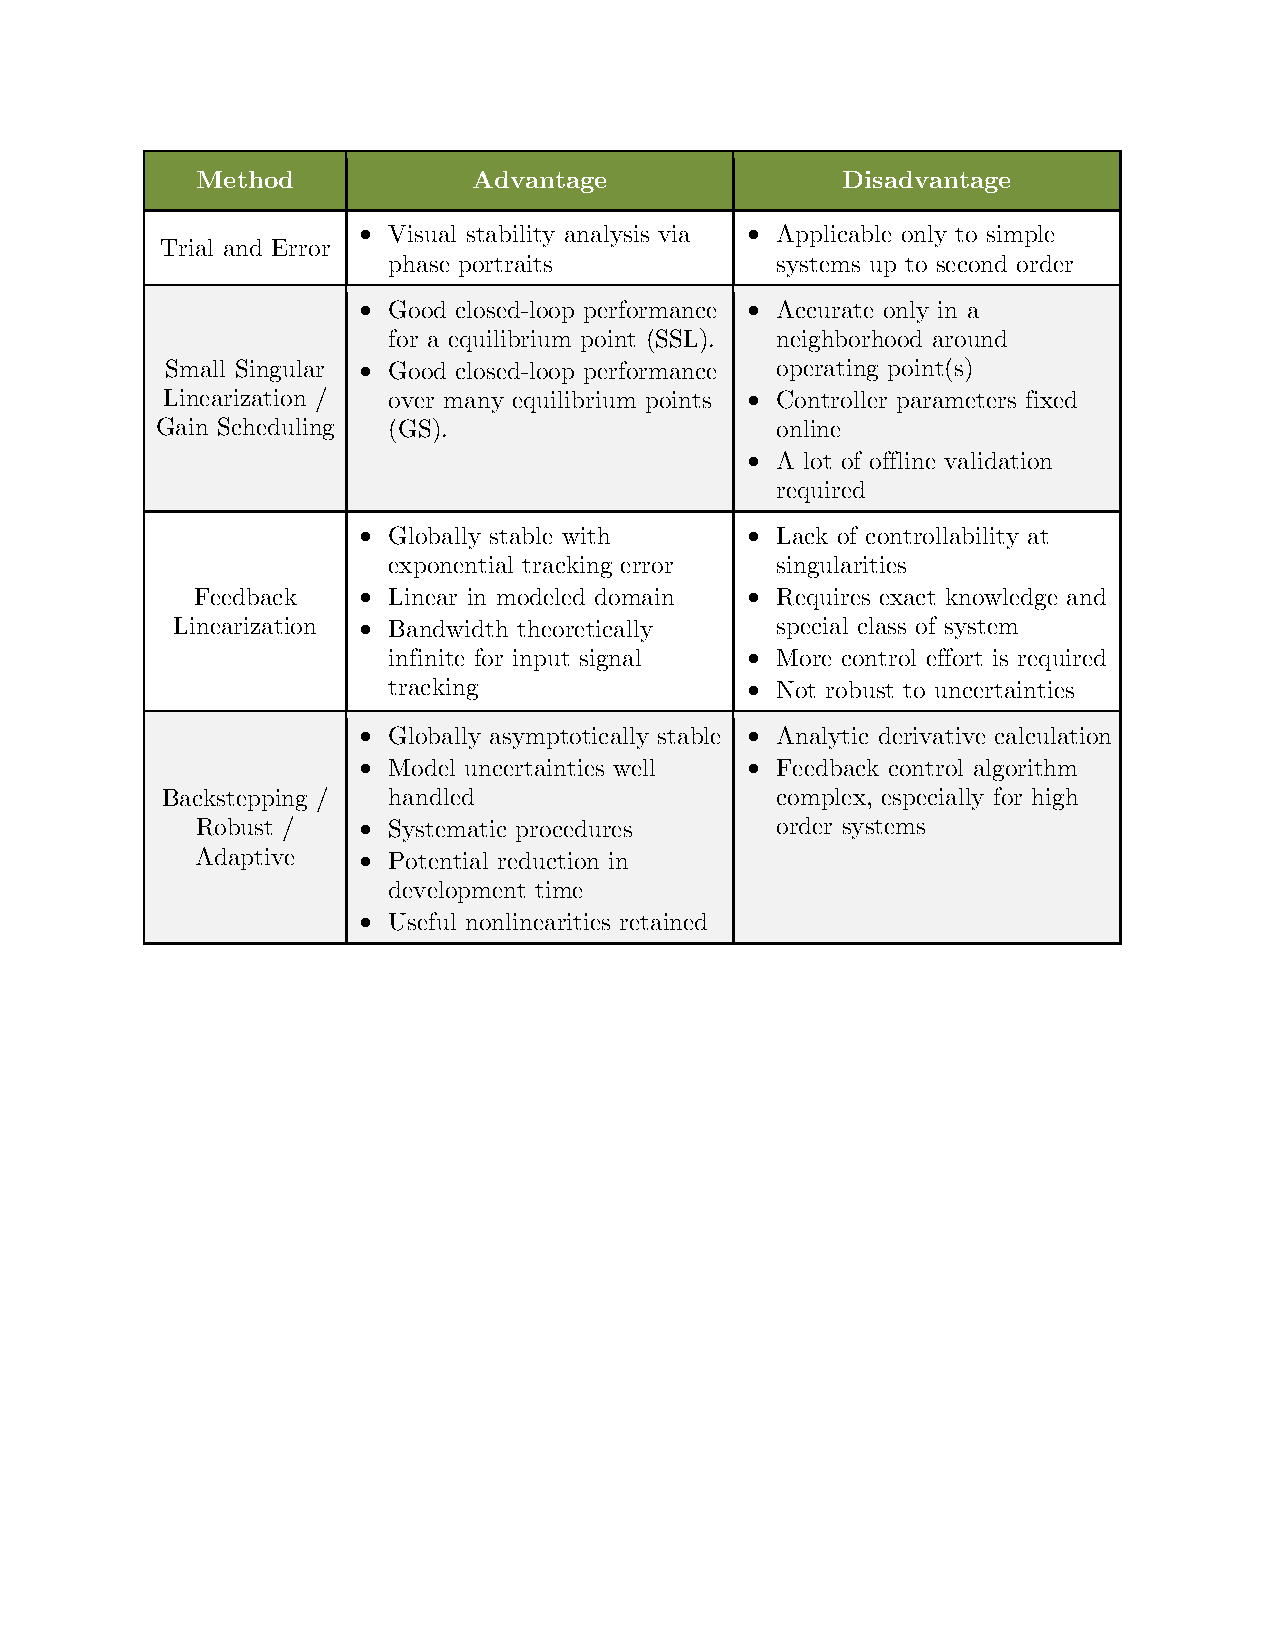
\includegraphics[scale=0.95]{tables/really_stupid_table.pdf}
	%	\end{adjustwidth}
		\label{tab: nonlinear_methods}%
	\end{table}

But how is feedback linearization better than small singular linearization for the same equilibrium point, especially since both systems are linear? In the former, exact state transformations and nonlinear feedback are used, rather than the latter where linear \textit{approximations} of the nonlinear system and linear feedback are used. The downside is that all nonlinearities must be precisely known.  Furthermore, even the ``worst case performance attained by a nonlinear controller coincides with the performance attained by the best linear design.'' \citet[Linear Versus Nonlinear]{Kokotovic1992}

%http://med.ee.nd.edu/MED7/med99/papers/MED115.pdf
``One of the main problems with applying feedback linearization techniques is that the process produces a system with the same \textbf{relative degree} as the original system, but usually with an order that is less. This process results in zero or internal dynamics, which are modes that are effectively rendered unobservable by the linearization process. If the system is non-minimum phase, then the zero dynamics are unstable. The analogy with linear systems is that a zero-pole system is linearized into an all-pole system by selecting the pole-zero excess as the order of the approximating system. In order to produce linearized systems that have no internal dynamics, techniques which preserve the dynamic order of the system are needed.'' \citet{Med99}

\subsection{Lyapunov Based Control Design}
\label{sub: lyapunov_based} %'flip of the coin' intro summarization of \citet{Slotine1991}
There are two ways to apply Lyapunov's direct method based on where you begin: \begin{inparaenum}[\itshape 1\upshape)] \item{If a control law is hypothesized then a valid Lyapunov function needs to be found to justify the choice.} \item{If a Lyapunov function is hypothesized then a control law needs to be found to make the Lyapunov function valid.}\end{inparaenum}~This section will apply the latter technique using a \textbf{control Lyapunov function} (CLF).%
\nomenclature[A]{CLF}{Control Lyapunov Function}% % %  N O M E N C L A T U R E  % % %

Up to this point Lyapunov theorems have been used to prove stability of a given system, however the main objective is to \textit{design} closed-loop systems with desirable stability properties. 
The following point by \citet{Freeman1996a} clearly summarizes the parallelism between Lyapunov functions and CLFs: ``Just as the existence of a Lyapunov function is necessary and sufficient for the stability of a system without inputs [closed-loop], the existence of a CLF is necessary and sufficient for the \textit{stabilizability} of a system with a control input.''

The ``control'' prefix implies that the nonlinear system it's applied to has an explicit dependence on $u$, that is:
%
	\begin{equation}
		\dot{\vect{x}}=\vect{f}(\vect{x},u) \quad,\quad \vect{x}\in \mathbb{R}^n \quad,\quad \vect{u}\in \mathbb{R} \quad,\quad \vect{f}(0,0)=0
		\label{eq: clf_f}
	\end{equation} 

If a stabilizing feedback control law $\stab(\vect{x})$ is chosen for control input $u$ such that the inequality in \autoref{eq: clf_vdot} holds, implying $\dot{\vect{x}}=\vect{f}(x,\stab(\vect{x}))$ where $\vect{x}=0$ is an equilibrium point, then the origin is globally asymptotically stable.
%
	\begin{equation}
		\dot{V}(\vect{x},\alpha)= \pd{V}{\vect{x}} \vect{f}(\vect{x},\stab(\vect{x})) \leq -W(\vect{x})
		\label{eq: clf_vdot}
	\end{equation} 
where $W(x)$ is a positive definite function; see \citet[Sec. 2.1.2]{Krstic95}.

\begin{defn}[Control Lyapunov Function (CLF)] \alignright \citet[Def. 2.4]{Krstic95},\citep{Harkegard2003}\\
A positive definite, radially unbounded, smooth scalar function $V = V(\vect{x})$ is called a CLF for $\dot{\vect{x}}=\vect{f}(\vect{x},u)$ if there exists a $u$ such that: \label{defn: clf}
	\begin{equation}
		\label{eq: clf_def} \inf_{u \in \mathbb{R}} \left\lbrace \dot{V}(\vect{x},u) = \pd{V}{\vect{x}} \vect{f}(\vect{x},u) < 0 \right\rbrace \quad,\quad \forall \, \vect{x} \neq 0
	\end{equation}
\end{defn}
%
\noindent where \textbf{inf} denotes infimum, the greatest lower bound. For systems affine in control, ie.
%
	\begin{equation}
		\dot{\vect{x}}=\vect{f}(\vect{x})+\vect{g}(\vect{x})u \quad,\quad \vect{f}(0)=0\,,
		\label{eq: clf_f_affine}
	\end{equation}
the CLF inequality in \autoref{eq: clf_vdot} becomes
%
	\begin{equation}
		\dot{V}(\vect{x},\stab)= \pd{V}{\vect{x}} \vect{f}(\vect{x}) + \pd{V}{\vect{x}} \vect{g}(\vect{x})\stab(\vect{x}) \leq -W(\vect{x})
		\label{eq: clf_vdot_affine}
	\end{equation} 

For this system the only way to satisfy \manref{Definition}{defn: clf} is if:
$$\pd{V}{\vect{x}} \vect{g}(\vect{x})=0 \quad \Rightarrow \quad \pd{V}{\vect{x}} \vect{f}(\vect{x}) < 0 \quad,\quad \forall \, \vect{x} \neq 0 $$

The problem with the CLF concept is that for most nonlinear systems it is unknown. ``The task of finding an appropriate CLF may be as complex as that of designing a stabilizing feedback law. For several important classes of nonlinear systems, we will solve these two tasks simultaneously using a backstepping procedure.'' \citet{Krstic95}

\subsection{Backstepping}
\label{sub: backstepping}
Key features of backstepping will be verified alongside implementation of the control architecture. Defining attributes and commonly mentioned benefits of backstepping are:
%
	\begin{table}[H]%
		\centering \label{tab: bstep_keywords}%
		\caption{Backstepping Key Terms}%
		\includegraphics[scale=0.95]{4_design/backstepping_keywords.pdf}%
	\end{table}%

Backstepping offers a systematic design procedure via the addition of integrators, and can handle various classes of nonlinear systems; two typical classes will be introduced based on presentation by \citet[Sec. 2.3.1]{Krstic95} and \citet[Sec. 3.3.2]{Harkegard2003}.

\begin{defn}[Strict Feedback System] \label{defn: strict_fb} ~\\
The first is a \textit{strict feedback} system and is of the form:
	\begin{equation} \label{eq: sys_strict_fb}
		\begin{aligned}   %equation + aligned vs. align => centered #
			\dot{x} 	\quad =& \quad  f_0(x) + g_0(x)\virt_1   					\\
			\dot{\virt}_1 	\quad =& \quad  f_1(x,\virt_1) 			+ g_1(x,\virt_1)\virt_2  											\\
			\dot{\virt}_2 	\quad =& \quad 	f_2(x,\virt_1,\virt_2) 	+ g_2(x,\virt_1,\virt_2)\virt_3 									\\
							\quad \vdots 											\\
			\dot{\virt}_{k-1}\quad =& \quad  f_{k-1}(x,\virt_1,\cdots,\virt_{k-1}) 	+ g_{k-1}(x,\virt_1,\cdots,\virt_{k-1})\virt_k 		\\
			\dot{\virt}_{k} \quad =& \quad  f_{k}(x,\virt_1,\cdots,\virt_{k}) 		+ g_{k}(x,\virt_1,\cdots,\virt_{k})u
		\end{aligned}
	\end{equation}
where $x \in \mathbb{R}^n$, $\virt_1,\cdots,\virt_{k}$ are scalar virtual control laws, and the $x$-subsystem satisfies assumptions necessary to apply backstepping, to be introduced in \manref{Assumption}{ass: bs}. The $\virt$-system is referred to as ``strict-feedback'' because ``nonlinearities $f_i$ and $g_i$ in the $\dot{\virt_i}$-equation ($i = 1,\cdots,k$) depend only on $x,\virt_1,\cdots,\virt_{i}$ that is, on state variables that are fed back.'' 
\end{defn}

\begin{defn}[Pure Feedback System] \label{defn: pure_fb} ~\\
The second is a \textit{pure feedback} system and is of the form:
	\begin{equation} \label{eq: sys_pure_fb}
		\begin{aligned}
			\dot{x} 			\quad =& \quad  	f_0(x,\virt_1)  				\\
			\dot{\virt}_1 		\quad =& \quad  	f_1(x,\virt_1,\virt_2)  				\\
			\dot{\virt}_2 		\quad =& \quad 		f_2(x,\virt_1,\virt_2,\virt_3)  		\\
								\quad \vdots  													\\
			\dot{\virt}_{k-1}  	\quad =& \quad  	f_{k-1}(x,\virt_1,\cdots,\virt_k)  	\\
			\dot{\virt}_{k} 	\quad =& \quad  	f_k(x,\virt_1,\cdots,\virt_{k},u)
		\end{aligned}
	\end{equation}
where $\virt_i \in \mathbb{R}^n$ and the $x$-subsystem again satisfies upcoming \manref{Assumption}{ass: bs}. The form of this system represents a more general class of ``triangular'' systems, specifically a lower triangular system. In comparison to strict-feedback systems, \manref{System}{eq: sys_pure_fb} lacks the \textit{affine}\footnote{An affine function is just a linear function plus a translation term.} appearance of variables $\virt_k$ and $u$. 
\end{defn}

\citet[Sec. 2.3]{Krstic95} explicitly shows the recursive design procedures in which a \textbf{stabilizing control law} $\stab(x)$ is generated from a Lyapunov function $V$ for each intermediate \textbf{virtual control law} $\virt$; to be demonstrated in the derivation of the higher order backstepping controller in \manref{Sec.}{subsub: backstep_higher}.

The control architecture will first be applied to a general second order system, so that the reader may develop a sense of procedure and terminology. An extension of this special case to a higher order system will follow, where clear steps that characterize recursive application of the procedure will be defined.

\subsubsection{Second Order Systems}
\label{subsub: backstep_second}
Typically in feedback control architectures the objective is to create a control law that cancels known dynamics and impose variables that transform the system into a tracking problem. The key term here is \textit{known}, implying that complete model information is available. Feedback linearization is one such case, where the exact knowledge of \textit{nonlinear} system dynamics is required; if one of the functions is uncertain then cancellation is not possible. The key idea here is \textit{tracking}, with the goal of driving the error between an actual and desired value to zero.

Backstepping synthesis efficiently handles these two critical objectives. Stabilizing nonlinear terms in the dynamics, if recognized, may be retained hence less precise modeling information and less control effort is necessary. Also, the inclusion of nonlinearities improves transient performance.

To begin the backstepping\footnote{Alternatively referred to as \textit{integrator} backstepping.} procedure, we'll select a general first order system $(n=1)$, 
	\begin{equation}
		\dot{x}= f(x)+g(x)u \,,	
		\label{eq: bs_sys_1d}
	\end{equation}
and augment it with an integrator, thereby transforming it to a second order system:
	\begin{subequations} \label{eq: bs_sys_2d}
		\begin{align} 
			\label{eq: bs_sys_2da} \dot{x} 	\quad =& \quad f(x)+g(x)\virt \\
			\label{eq: bs_sys_2db} \dot{\virt} \quad =& \quad u
		\end{align}
	\end{subequations}
where $[x,\virt]^T \in \mathbb{R}^{n+1}$ is the state and $u \in \mathbb{R}$ is the control input. The function $f:\mathcal{D} \to \mathbb{R}^n$ and $g:\mathcal{D} \to \mathbb{R}^n$ are smooth in a domain $\mathcal{D} \subset \mathbb{R}^n$ that contains $x=0$ and $f(0)=0$. The \textbf{main objective} is to design a state feedback control law $u$ to force $\virt$ to perform either \begin{inparaenum}[\itshape 1\upshape)] \item{regulation by stabilizing the origin $(x = 0 \,, \virt = 0)$, ie. $x(t) \to 0$ as $t \to \infty$, or} \item{tracking by causing the $x$-portion of the state to track a reference signal, say $y_d$, ie.  $x(t) \to y_d$ as $t \to \infty$} \end{inparaenum}; with respect to \manref{System}{eq: bs_sys_1d}, ``this is equivalent to treating $\virt$ as a \textit{virtual control} input for the $\dot{x}$ equation,'' hence we call $\virt$ a virtual control law. The same idea can be found in cascaded control design, as \manref{System}{eq: bs_sys_2d} may be viewed as the cascade connection of $\dot{x}$ and $\dot{\virt}$ subsystems. This is shown in \manref{Figure}{fig: bs_blockdiagram}[\textit{a})], where again the first equation treats $\virt$ as a ``control input,'' the second equation is the integrator, and the dashed box is the original system in \autoref{eq: bs_sys_1d}.

For simplification, hence comprehensibility, backstepping for the regulation task will be derived herein. If the objective is tracking an exceptional derivation is provided in \citet[Sec. 5.3.1]{Farrell2006}. The corresponding assumptions are:
\begin{ass}[\textit{Integrator} Backstepping] \alignright
	\vspace{1em}
	\begin{itemize}[labelindent=\parindent,leftmargin=.5in,noitemsep,nosep]
		\begin{minipage}{0.5\linewidth}
			\item Full state feedback
			\item System in Lower-Triangular form*
			\item System parameters $f$ and $g$ known*
		\end{minipage}
		\begin{minipage}{0.5\linewidth}
			\item Smooth, positive definite CLF known*
			\item Smooth state feedback control $u$
			\item[] ~
		\end{minipage}
	\end{itemize} \label{ass: backstepping1}
	\alignright *\textit{\small{specific to this flavor of backstepping}}
\end{ass}

Suppose that \manref{Subsystem}{eq: bs_sys_2da} can be stabilized by a state feedback control $\stab(x)$,
	\begin{equation*}
		\virt = \stab(x) \quad \Rightarrow \quad \dot{x} = f(x)+g(x)\stab(x)
		\label{eq: bs_step1}
	\end{equation*}
and further that a Lyapunov function is known that renders the equilibrium point, or origin in this case, asymptotically stable, $\stab(0)=0$:
	\begin{equation}
		\dot{V}(x) = \pd{V}{x}\dot{x} = \pd{V}{x} \left[ f(x)+g(x)\stab(x) \right] \leq -W(x) \quad,\quad \forall \, x \in \mathcal{D}
		\label{eq: bs_v}
	\end{equation}
where $W(x)$ is a positive definite function. By adding and subtracting the term involving the stabilizing function, $\pm g(x)\stab(x)$, from the first equation in \manref{System}{eq: bs_sys_2d}, we obtain the equivalent system below, as shown in \manref{Figure}{fig: bs_blockdiagram}[\textit{b})]:
	\begin{subequations} \label{eq: bs_step2}
		\begin{align}
			\label{eq: bs_step2a} \dot{x} 	\quad =& \quad \left[ f(x)+g(x)\stab(x) \right] + g(x) \left[ \virt - \stab(x) \right] \\
			\label{eq: bs_step2b}	\dot{\virt} \quad =& \quad u
		\end{align}
	\end{subequations}
%
	\begin{figure}[htbp]
		\centering
		\begin{overpic}[scale=1]%[scale=1,grid,tics=10]
			{4_design/backstepping_blockdiagram.pdf}
			\put(38,70){\autoref{eq: bs_sys_2da}}
			\put(39,4){\autoref{eq: bs_step4a}}
		\end{overpic}
		\caption{Backstepping Block Diagram Representation: \textit{a}) Integral augmented cascade system \textit{b}) introducing $\pm \stab(x)$  \textit{c}) ``backstepping'' $-\stab(x)$ through the integrator}%
		\label{fig: bs_blockdiagram}%
	\end{figure}
%
\indent If we let $z$ be the \textbf{error state}, or deviation of actual from desired virtual control with the latter achieved via a stabilizing function $\stab(x)$,
	\begin{equation}
		z = \virt - \virt_{des} =\virt - \stab(x)
		\label{eq: bs_z}
	\end{equation}
then a transformed system, \ref{eq: bs_step3}, is obtained by \begin{inparaenum}[\itshape a\upshape)] \item{substitution of \autoref{eq: bs_z} into \manref{Subsystem}{eq: bs_step2a} and} \item{the derivative\footnote{$z$ is a function of $x$ only, hence we may use the sum rule for differentiation: $\dot{z} = {d\virt}/{dx} - {d\stab}/{dx} = u - \dot{\stab}$} of \autoref{eq: bs_z}} \end{inparaenum}:
	\begin{subequations} \label{eq: bs_step3}
		\begin{align}
			\label{eq: bs_step3a} \dot{x} 	\quad =& \quad \left[ f(x)+g(x)\stab(x) \right] + g(x)z \\
			\label{eq: bs_step3b} \dot{z} 	\quad =& \quad  u - \dot{\stab}
		\end{align}
	\end{subequations}
as depicted in \manref{Figure}{fig: bs_blockdiagram}[\textit{c})]. The term backstepping is derived from the procedure leading to \manref{System}{eq: bs_step3}, whereby taking the derivative of $z$ led to ``backstepping'' of $-\stab(x)$ through the integrator; this defining feature is highlighted in \manref{Figures}{fig: bs_blockdiagram}[\textit{b})] and \hyperref[{fig: bs_blockdiagram}]{\textit{c})}. A key feature of backstepping is that we don't use a differentiator to implement the time derivative $\dot{\stab}$ ; since $f$, $g$, and $\stab$ are known, the derivative $\dot{\stab}$ may be computed offline, ie. analytically, without the need of a differentiator by using the chain rule:
	\begin{equation}
		\dot{\stab} = \pd{\stab}{x}\dot{x} = \pd{\stab}{x}\left[ f(x)+g(x)\virt \right]
		\label{eq: bs_stab_dot}
	\end{equation}
%
\indent If we introduce a \textit{modified control input} by defining $v = u - \dot{\stab}$ then the \manref{System}{eq: bs_step3} may be reduced to
	\begin{subequations}%
		\begin{align}%
			\label{eq: bs_step4a} \dot{x} 	\quad =& \quad \left[ f(x)+g(x)\stab(x) \right] + g(x)z \\
			\label{eq: bs_step4b} \dot{z} 	\quad =& \quad v
		\end{align}%
	\end{subequations}%
%
\indent This is nearly the same as \manref{System}{eq: bs_sys_2d}, except that the inclusion of a stabilizing function $\stab$ and change of variables to $xz$ causes the first equation in this cascade system to have an asymptotically stable origin when the input is zero. If we use
	\begin{equation}
		\begin{aligned}
			V(x,z) = V(x) + \frac{1}{2}z^2
		\end{aligned}
		\label{eq: bs_step5}
	\end{equation}
as a control Lyapunov function (CLF) and find the total derivative,
	\begin{equation}
		\begin{aligned}
			\dot{V} \quad =& \quad \pd{V}{x}\frac{dx}{dt} + \pd{V}{z}\frac{dz}{dt} \\
					\quad =& \quad \pd{V}{x} \left\lbrace \left[ f(x)+g(x)\stab(x) \right] + g(x)z \right\rbrace + \pd{V}{z}v \\
					\quad \leq& \quad -W(x) + \pd{V}{x}g(x)z + zv
		\end{aligned}
		\label{eq: bs_step6a}
	\end{equation}
where \autoref{eq: bs_v} was utilized to make the $-W(x)$ substitution, then choosing a modified control input $v$
	\begin{equation}
			v = -\pd{V}{x}g(x) - kz \quad,\quad k>0
		\label{eq: bs_step7}
	\end{equation}
and substituting this back into \autoref{eq: bs_step6a} implies
	\begin{equation}
			\dot{V} \leq -W(x) - kz^2
		\label{eq: bs_step6b}
	\end{equation}
%
\indent $\dot{V}$ proves that in the $(x,z)$ coordinates the equilibrium point, or origin in this case, $(x=0 \,, z=0)$ is asymptotically stable. Since we chose $\stab(0)=0$, we may conclude that from \autoref{eq: bs_z} the origin $(x=0 \,, \stab=0)$ is also asymptotically stable. The final step is substituting $\dot{z}=v$ and $\dot{\stab}$ into \manref{Subsystem}{eq: bs_step3b} and rearranging in order to obtain the state feedback control law, $u$, for the second order system we started from:
	\begin{equation}
			u = \dot{\stab} + \dot{z} = \pd{\stab}{x}\left[ f(x)+g(x)\virt \right] - \pd{V}{x}g(x) - kz
		\label{eq: bs_step8}
	\end{equation}

Further, if all items in \manref{Assumption}{ass: backstepping1} hold and $V(x)$ is radially unbounded then the equilibrium point is globally asymptotically stable. This process is summarized formally by \manref{Assumption}{ass: backstepping2} and \manref{Lemma}{lem: bs}:

\begin{ass}[Backstepping Stabilizing Function] \alignright \citet[Asmp. 2.7]{Krstic95} \label{ass: bs}\\
For the general first order system
	\begin{equation} 
		\dot{x} = f(x) + g(x)u \quad,\quad f(0)=0
		\label{eq: bs_ass_sys}
	\end{equation}
where $x \in \mathbb{R}^n$ is the state and $u \in \mathbb{R}$ is the control input. There \textbf{exists} a continuously differentiable feedback control law, called a stabilizing function $\stab(x)$
	$$ u = \stab(x) \quad,\quad \stab(0)=0 $$
and a smooth, positive definite, radially unbounded function $V: \mathbb{R}^n \rightarrow \mathbb{R}$ such that
	$$ \dot{V} = \pd{V}{x}\left[ f(x) + g(x)\stab(x) \right] \leq -W(x) \leq 0 \quad,\quad \forall\; x \in \mathbb{R}^n $$
where $W: \mathbb{R}^n \rightarrow \mathbb{R}$ is positive semidefinite.
\label{ass: backstepping2}
\end{ass}

With \manref{Theorem}{thm: lasalle-yoshi}[LaSalle-Yoshizawa] the control law in \manref{Assumption}{ass: backstepping2} guarantees global boundedness of $x(t)$ via the regulation of $W(x(t))$:
	$$ \lim\limits_{t\to\infty} W(x(t)) = 0 $$
Furthermore, a stronger convergence result is achievable if \manref{Theorem}{thm: lasalle}[LaSalle] is satisfied with $W(x)$ is positive definite, the control renders $x=0$ the GAS equilibrium of \autoref{eq: bs_ass_sys}.

\begin{lem}[Backstepping] \alignright \citet[Lem. 2.8]{Krstic95} \label{lem: bs} \\
Let \autoref{eq: bs_ass_sys} be augmented by an integrator:
	\begin{subequations} \label{eq: lem_bs_sys}%
		\begin{align}
			\label{eq: lem_bs_sys_a} \dot{x} 	\quad =& \quad f(x) + g(x)\virt \\
			\label{eq: lem_bs_sys_b}\dot{\virt} \quad =& \quad u \,,
		\end{align}
	\end{subequations}
and suppose that \manref{Subsystem}{eq: lem_bs_sys_a} satisfies \manref{Assumption}{ass: backstepping2} with $\virt = \mathbb{R}$ as its control.
%
	\begin{enumerate}[noitemsep,nosep,labelindent=\parindent,leftmargin=\parindent]%
	%
	\renewcommand{\labelenumi}{\roman{enumi}) }
	%
	\item{If $W(x)$ is \textbf{positive definite}, then
		\begin{equation} \label{eq: bs_lem_w}
			V(x,\virt)= V(x) + \frac{1}{2}[\virt - \stab(x)]^2
		\end{equation}
	is a CLF for \manref{System}{eq: lem_bs_sys}, that is, there exists a feedback control $u=\stab(x,\virt)$ which renders \textbf{the origin} $\mathbf{(x=0,\virt=0)}$ the GAS equilibrium point. One such control is
		\begin{equation} \label{eq: bs_lem_u}
			u = \pd{\stab}{x}\left[ f(x)+g(x)\virt \right] - \pd{V}{x}g(x) - k[\virt - \stab(x)] \quad,\quad k>0 %
		\end{equation}}
	\item{If $W(x)$ is \textbf{positive semi-definite}, then there exists a feedback control which renders $\dot{V} \leq -W(x,\virt) \leq 0$, such that $W(x,\virt) > 0$ whenever $W(x)>0$ or $\virt \neq \stab(x)$. This guarantees global boundedness and convergence of $[x(t),\virt(t)]^T$ to the largest invariant set $\mathcal{M}$ contained in the set $\mathcal{E} = \left\lbrace [x,\virt]^T \in \mathbb{R}^{n+1} \quad|\quad W(x)=0 \,,\, \virt = \stab(x) \right\rbrace $}
	\end{enumerate}
\end{lem}

``The \textbf{main result of backstepping} is not the specific form of the control law, \autoref{eq: bs_lem_u}, but rather the construction of a Lyapunov function whose derivative can be made negative definite by a wide variety of control laws.'' \citet{Krstic95}.

This result may be extended to systems with a chain of integrators in a systematic fashion. ``The only difference is that there will be more virtual states to ``backstep'' through. Starting with the ``farthest'' from the actual control, each step of the backstepping technique can be broken up into three parts:'' \citet{Sonneveldt2007}
\begin{defn}[Constructive Nature of Backstepping - Design Procedure]~\\
\vspace{-2em}
	\begin{enumerate}[labelindent=\parindent,leftmargin=\parindent,noitemsep,nosep]
		\item \textit{Introduce a virtual control $\virt = \stab(x)$, an error state $z$, and rewrite the current state equation in terms of these}
		\item \textit{Choose a CLF for the system, treating it as a final stage}
		\item \textit{Choose an equation for the virtual control that makes the CLF stabilizable}
	\end{enumerate} 
\end{defn}
\nomenclature[*n]{$\virt$}{Virtual Control Law \nomunit{BS}}% % %  N O M E N C L A T U R E  % % %
\nomenclature[*a]{$\alpha(x)$}{Stabilizing Feedback Control Law \nomunit{BS}}% % %  N O M E N C L A T U R E  % % %
\nomenclature[-]{$z$}{Tracking Error \nomunit{BS}}% % %  N O M E N C L A T U R E  % % %
\nomenclature[+]{$W$}{Positive (Semi-)Definite Function \nomunit{BS}}% % %  N O M E N C L A T U R E  % % %
\nomenclature[A]{BS}{Backstepping}% % %  N O M E N C L A T U R E  % % %

The following examples will show how control law and control Lyapunov function (CLF) selection effects control design. In \manref{Example}{eg: bs_useful}, it will shown how recognition of useful nonlinearities in Lyapunov based control design leads to a more efficient control law than one designed via feedback linearization. In \manref{Example}{eg: bs_lyp}, backstepping will be applied to the same system to demonstrate the technique and show the flexibility in this procedure.

\begin{eg}[Useful Nonlinearities] \alignright \citet[Ex. 3.1]{Harkegard2003} \label{eg: bs_useful}\\
	\indent Consider the system
		\begin{equation} \label{eq: bs_ex_sys}
			\dot{x} = -x^3 + x + u
		\end{equation}
	and let $x=0$ be the \textit{desired} equilibrium point. The unforced dynamics, $u=0 \,\therefore\, \dot{x}=-x^3+x$, are depicted via the phase portrait in \autoref{fig: bs_ex1}. 

	\begin{figure}[tb]%
		\begin{adjustwidth}{-1in}{-1in}% adjust the L and R margins by 1 inch
			\centering%
			\includegraphics[scale=.9]{4_design/bs_ex_pp.pdf}%
		\end{adjustwidth}%
		\caption{Composite Phase Portrait for \manref{System}{eq: bs_ex_sys} with $u=0$}%
		\label{fig: bs_ex1}%
	\end{figure}
	
	Note that this is a 1D phase portrait, unlike the 2D phase portraits illustrated in \autoref{subsec: eqm}; the differential equation is represented as a vector field on the x-axis, determined by the velocity  $\dot{x}$ at each $x$. A physical way to understand this is to imagine fluid flowing along the x-axis with a velocity that varies according to \manref{System}{eq: bs_ex_sys}; \citet{Strogatz1994}. If $\dot{x}<0$ then the flow is to the left and to the right if $\dot{x}>0$. Equilibrium points coincide with x-axis intersections, as application of \autoref{eq: eqm_pt} dictates, and depending on the surrounding \textit{flow} will be stable or unstable. 
	
	For the desired equilibrium point, ie. the origin, ``to be asymptotically stable, the sign of $\dot{x}$ should be opposite that of x for all x.'' \autoref{fig: bs_ex1} shows the linear term, $+x$, dominates and de-stabilizes near the origin (dashed gray line), while the cubic term, $-x^3$, dominates and stabilizes for values of $x$ outside of $\pm1$. Remember that these observations are for the unforced form of \manref{System}{eq: bs_ex_sys}. Developing a stabilizing control law, ie. working with the forced form of the system, will transform the dynamics to make a stable operating point coincident with the origin; in the phase portrait we would see a single, stable equilibrium point at the origin and system trajectory only occupying quadrants II and IV.
	
	We begin \textbf{Lyapunov based control} law development by recognizing that ``to make the origin GAS only the linear dynamics need to be counteracted by the control input. This can be achieved by selecting
		\begin{equation} \label{eq: bs_ex_u}
			u = -x
		\end{equation}
	and a CLF given by 
		\begin{equation} \label{eq: bs_ex_V}
			V(x) = \frac{1}{2}x^2
		\end{equation}
	which yields
		\begin{equation} \label{eq: bs_ex_Vdot}
			\dot{V}(x) = \pd{V}{x}\dot{x} = x(-x^3+x+u) = -x^4
		\end{equation}
	proving the origin is GAS according to \manref{Cor.}{cor: barbashin-krasovskii}[Barbashin-Krasovskii].''
	
	Alternatively, applying \textbf{feedback linearization} requires that the control law counteracts all nonlinear dynamics:
		\begin{equation} \label{eq: fb_ex_u}
			u = x^3 - kx \quad,\quad k>1
		\end{equation}
	As mentioned previously, this control law does not recognize the naturally stabilizing nonlinear term, $-x^3$, in fact it counteracts it thus requiring more control effort in contrast to $u=-x$.
\end{eg}

\begin{eg}[Flexibility in Backstepping] \alignright \citet[Ex. 3.1]{Harkegard2003} \label{eg: bs_lyp}\\
	\indent Consider \manref{System}{eq: bs_ex_sys} in the previous example augmented by an integrator where $x = x_1$ and $\virt = x_2$.
		\begin{subequations}%
			\label{eq: bs_ex2_sys}%
			\begin{align}%
				\label{eq: bs_ex2_sysa} \dot{x}_1 \quad =& \quad -x_1^3 + x_1 + x_2 \\
				\label{eq: bs_ex2_sysb} \dot{x}_2 \quad =& \quad u
			\end{align}%
		\end{subequations}%
	\indent The first task is to stabilize the equilibrium point of \manref{Subsystem}{eq: bs_ex2_sysa} by treating $x_2$ as a virtual control input. Since we know from phase portrait observations in \autoref{fig: bs_ex1} that $-x_1^3$ is a useful nonlinearity we set out to preserve this term. The objective is to choose a stabilizing function $\stab(x_1)$ that cancels the de-stabilizing linear term $x_1$, just as the control law $u$ in \autoref{eq: bs_ex_u} did:
		\begin{equation} \label{eq: bs_ex2_virt}
			{x_2}_{des} \equiv \stab(x_1) = -x_1
		\end{equation}
		\nomenclature[B]{$des$}{Desired}%
	Next, the error variable $z$ is introduced, which is defined as the difference between actual and desired virtual control.
		\begin{equation} \label{eq: bs_ex2_z}
			z = x_2 - \stab(x_1) = x_2 + x_1
		\end{equation}
	Now we can rewrite the system in $xz$ coordinates with substitution of \ref{eq: bs_ex2_z} into \ref{eq: bs_ex2_sysa} and the analytic derivative of $z$, ie. $\dot{z} = \dot{x}_2 + \dot{x}_1$ with substitution of \ref{eq: bs_ex2_sysb}:
		\begin{subequations} \label{eq: bs_ex2_xz}
			\begin{align}
				\dot{x}_1 \quad =& \quad  -x_1^3 + z \\
				\dot{z} \quad =& \quad  u - x_1^3 + z
			\end{align}
		\end{subequations}
	\indent Following \manref{Backstepping Lemma}{lem: bs}, a CLF is now constructed for \manref{System}{eq: bs_ex2_xz}. Our initial choice will reuse the positive definite quadratic postulated in \autoref{eq: bs_ex_V} for the first term of \manref{CLF}{eq: bs_lem_w} in the lemma.
		\begin{equation} \label{eq: bs_ex2_V}
			V(x_1) = \frac{1}{2}x_1^2
		\end{equation}
	Including the penalizing term for the deviation from the stabilizing function yields
		\begin{equation} \label{eq: bs_ex2_V2}
			V(x_1,x_2) = V(x_1) + \frac{1}{2}(x_2 - \stab(x_1))^2 = \frac{1}{2}x_1^2 + \frac{1}{2}z^2
		\end{equation}
	Differentiating with respect to time will allow us to evaluate which choices for $u$ satisfy Lyapunov stability theorems
		\begin{equation} \label{eq: bs_ex2_Vdot}
			\dot{V} = x_1(-x_1^3+z) + z(u-x_1^3+z) = -x_1^4 + z(x_1+u-x_1^3+z)
		\end{equation}
	In order to ``render $\dot{V}$ negative definite, $u$ must dominate the $z$ term using a control input of, eg. $-3z$. In addition, since the mixed terms between $x_1$ and $z$ are indefinite, there seems to be no other choice than to cancel them using the control law''
		\begin{equation} \label{eq: bs_ex2_u}
			u = x_1^3 - x_1 -3z
		\end{equation}	
	\indent This choice however, does not recognize the fact that the $-x_1^3$ term in subsystem is naturally stabilized outside of $x_1=\pm1$. We can do better by choosing a different $V(x_1)$; instead of specifying a CLF beforehand, we will leave $V(x_1)$ alone and let its formulation fall out of the backstepping design process. This is the reason as to why backstepping is considered a \textbf{flexible design procedure}. Consider \manref{CLF}{eq: bs_lem_w} again 
		\begin{equation} \label{eq: bs_ex2_V3}
			V(x_1,x_2) = V(x_1) + \frac{1}{2}(z)^2
		\end{equation}	
	and compute its derivative without presuming $V(x_1)$ known
		\begin{equation} \label{eq: bs_ex2_Vdot2}
			\begin{aligned}
				\dot{V} 	\quad=&\quad \pd{V}{x_1}\frac{d x_1}{d t} + \pd{V}{x_2}\frac{d x_2}{d t}\\
							\quad=&\quad \dot{V}(-x_1^3+z) + z(u - x_1^3 + z) \\
							\quad=&\quad -\dot{V}x_1^3 + z(\dot{V} + u - x_1^3 + z)
			\end{aligned}
		\end{equation}
	\indent Now we are able to choose a $V(x_1)$ such that $\dot{V}$ in \ref{eq: bs_ex2_Vdot2} cancels the indefinite mixed terms. This is achieved by selecting
		\begin{equation} \label{eq: bs_ex2_niceeee}
			\dot{V}(x_1) = x_1^3 \qquad \ni \qquad V(x_1) = \frac{1}{4}x_1^4
		\end{equation}
	With this CLF, \ref{eq: bs_ex2_Vdot2} is now
		\begin{equation} \label{eq: bs_ex2_Vdot3}
			\dot{V} = -x_1^6 + z(u+z)
		\end{equation}	
	In contrast to \autoref{eq: bs_ex2_Vdot} it is clear that the control law $u$ no longer needs to unnecessarily cancel the $-x_1^3$ term, in fact now we can build a linear control law in $x_1$ and $x_2$
		\begin{equation} \label{eq: bs_ex2_u2}
			u = -3z = -3x_1 -3x_2
		\end{equation}
	which renders $\dot{V} = -x_1^6 - 2z_2^2$ negative definite, thereby making the origin GAS. This technique for choosing $V(x_1)$ was published in \citet{Krstic1998}.
\end{eg}

\subsubsection{Higher Order Systems}
\label{subsub: backstep_higher}

Lower order system backstepping concepts may be extended to higher order systems, for which simplicity is maintained via recursive application of integrator backstepping. The aim of this section is to exemplify this procedure for a third order, $n=3$, system which applicable to any systems over an order of two.

\begin{eg}[Recusrive Nature of Backstepping] \alignright \citet[Ex. 13.7]{Khalil1996} \label{eg: bs_rec}\\
	\indent Consider the third-order system,
		\begin{subequations}%
			\label{eq: bs_ex3_sys}%
			\begin{align}%
				\label{eq: bs_ex3_sysa} \dot{x}_1 \quad =& \quad x_1^2 - x_1^3 + x_2 \\
				\label{eq: bs_ex3_sysb} \dot{x}_2 \quad =& \quad x_3 \\
				\label{eq: bs_ex3_sysc} \dot{x}_3 \quad =& \quad u
			\end{align}%
		\end{subequations}%
	which is nearly identical to \manref{System}{eq: bs_ex2_sys} however it's further altered by an additional integrator and $x_1$ is now squared. Each step below divides the procedure into a series of virtual control law solutions, with the final step defining the true control input $u$.
	
	\noindent \textbf{Step 1}: As with \manref{Example}{eg: bs_lyp}, we begin by developing a stabilizing feedback control $x_2 \equiv \stab(x_1)$ for \manref{Subsystems}{eq: bs_ex3_sysa} and \ref{eq: bs_ex3_sysb}. We may consider $x_3$ as the control input ``$u$''  that stabilizes the origin $x_1=0$; necessary in order to draw from \manref{Assumption}{ass: bs} and \manref{Lemma}{lem: bs}.
		\begin{subequations} \label{eq: bs_ex3_sys1}
			\begin{align} 
				\dot{x}_1 \quad =& \quad x_1^2 - x_1^3 + x_2 \\
				\dot{x}_2 \quad =& \quad x_3
			\end{align}
		\end{subequations}
	Choosing a stabilizing function, again that recognizes $-x_1^3$ as stabilizing,
		\begin{equation} \label{eq: bs_ex3_step1}
			\stab(x_1) = -x_1^2 - x_1
		\end{equation}
	leads to the reformulated system
		\begin{equation} \label{eq: bs_ex3_sysaa}
			\dot{x}_1 = -x_1 - x_1^3
		\end{equation}
	Note that the error state is defined as
		\begin{equation} \label{eq: bs_ex3_step2}
			z = x_2 - \stab(x_1) = x_2  -x_1^2 - x_1
		\end{equation}
	\indent If we chose the CLF $V(x_1) = \displaystyle \frac{1}{2}x_1^2$ and take the derivative
		\begin{equation} \label{eq: bs_ex3_V1}
			\dot{V} = \pd{V}{x_1}\dot{x}_1 =-x_1^2 -x_1^4 \leq -x_1^2 \quad,\quad \forall \, x_1 \in \mathbb{R}
		\end{equation}
	then apply $u$ and $V$ from \manref{Lemma}{lem: bs} to build the control $x_3$, with $f=x_1^2 - x_1^3$, $g=1$, and $k=1$,
		\begin{equation} \label{eq: bs_ex3_3a}
		\begin{aligned}
			x_3	\quad =& \quad \pd{\stab}{x_1}\left( x_1^2 - x_1^3 + x_2 \right) - \pd{V}{x_1} - [x_2 - \stab(x_1)] \\
				\quad =& \quad -(2x_1 + 1)(x_1^2 - x_1^3 + x_2) - x_1 - (x_2 + x_1^2 + x_1)
		\end{aligned}
		\end{equation}
	that stabilizes the origin $x=0$ globally to form the composite Lyapunov function
		\begin{equation} \label{eq: bs_ex3_step3b}
			V(x_1,x_2) = \frac{1}{2}x_1^2 + \frac{1}{2}(x_2  -x_1^2 - x_1)^2
		\end{equation}	
	
	\noindent \textbf{Step 2}: We now consider the next subsystem, \ref{eq: bs_ex3_sysc}, by viewing the third order system as a special case of \manref{System}{eq: bs_step2}
		\begin{align*} 
			\dot{x} 	\quad =& \quad f(x)+g(x)\virt \\
			\dot{\virt} \quad =& \quad u
		\end{align*}
	with the system in Step 1 condensed into
		\begin{equation} \label{eq: bs_ex3_3Dto2D}
			x = \left[ \begin{array}{c} x_1 \\ x_2 \end{array} \right] \quad,\quad f= \left[ \begin{array}{c} x_1^2-x_1^3+x_2 \\ 0 \end{array} \right] \quad,\quad g = \left[ \begin{array}{c} 0 \\ 1 \end{array}\right] \quad,\quad \virt=x_3 
		\end{equation}
	We know from Step 1 that the following feedback control, $x_3 \equiv \stab(x_1,x_2)$, and CLF stabilizes \manref{System}{eq: bs_ex3_sys1} 
		\begin{gather*} 
			\stab(x_1,x_2) 	=  -(2x_1 + 1)(x_1^2 - x_1^3 + x_2) - x_1 - (x_2 + x_1^2 + x_1) \\
			V(x_1,x_2)    	= \frac{1}{2}x_1^2 + \frac{1}{2}(x_2  -x_1^2 - x_1)^2
		\end{gather*} \label{eq: bs_ex3_stab2}
	which we define as the virtual control and portion of the CLF for \ref{eq: bs_ex3_3Dto2D}. Next, \manref{Backstepping Lemma}{lem: bs} is applied in order to obtain the globally stabilizing feedback control
		\begin{equation} \label{eq: bs_ex3_step4a}
			u = \pd{\stab}{x_1}(x_1^2 - x_1^3 + x_2) + \pd{\stab}{x_2}(x_3) - \pd{V}{x_2} - [x_3 - \stab(x_1,x_2)] 
		\end{equation}		
	and corresponding Lyapunov function
		\begin{equation} \label{eq: bs_ex3_step4b}
			V(x) = V(x_1,x_2) + \frac{1}{2}(x_3  -\stab(x_1,x_2))^2
		\end{equation}	
\end{eg}

This example is now \textbf{summarized for a more general form} of \manref{System}{eq: bs_sys_2d}
	\begin{subequations} \label{eq: bs_ho_sys}
		\begin{align} 
			\label{eq: bs_ho_sysa} \dot{x} 	\quad =& \quad f(x)+g(x)\virt \\
			\label{eq: bs_ho_sysb} \dot{\virt} \quad =& \quad f_a(x,\virt)+g_a(x,\virt)u
		\end{align}
	\end{subequations}
%TODO: what does the subscript a mean? A: Just a different function?
where $f_a$ and $g_a$ are smooth, and $g_a(x,\virt) \neq 0$ over the domain of interest. We may use the control input 
	\begin{equation} \label{eq: bs_ho_u}
		u = \frac{1}{g_a(x,\virt)}\left[ u_a -  f_a(x,\virt) \right] 
	\end{equation}
which reduces \manref{Subsystem}{eq: bs_ho_sysb} to the ``integrator form'' $\dot{\virt} = u_a$. If \manref{Backstepping Lemma}{lem: bs} conditions are satisfied by a stabilizing function $\stab(x)$ and Lyapunov function $V(x)$ then the Lemma combined with \autoref{eq: bs_ho_u} yields the stabilizing state feedback control
	\begin{equation} \label{eq: bs_ho_stab}
		u = \stab_a(x,\virt) = \frac{1}{g_a(x,\virt)} \left\lbrace  \pd{\stab}{x}\left[ f(x)+g(x)\virt \right] - \pd{V}{x}g(x) - k[\virt - \stab(x)] - f_a(x,\virt) \right\rbrace
	\end{equation}
for some $k > 0$ and the Lyapunov function
	\begin{equation} \label{eq: bs_ho_V}
		V_a(x,\virt) = V(x) + \frac{1}{2}\left[ \virt - \stab(x) \right]^2 
	\end{equation}
for \manref{System}{eq: bs_ho_sys}. By recursive application of backstepping, we can stabilize strict feedback systems as shown in \manref{Definition}{defn: strict_fb}:
\begin{equation} \tag{\ref{eq: sys_strict_fb}}
	\begin{aligned}   %equation + aligned vs. align => centered #
		\dot{x} 	\quad =& \quad  f_0(x) + g_0(x)\virt_1   					\\
		\dot{\virt}_1 	\quad =& \quad  f_1(x,\virt_1) 			+ g_1(x,\virt_1)\virt_2  											\\
		\dot{\virt}_2 	\quad =& \quad 	f_2(x,\virt_1,\virt_2) 	+ g_2(x,\virt_1,\virt_2)\virt_3 									\\
						\quad \vdots 											\\
		\dot{\virt}_{k-1}\quad =& \quad  f_{k-1}(x,\virt_1,\cdots,\virt_{k-1}) 	+ g_{k-1}(x,\virt_1,\cdots,\virt_{k-1})\virt_k 		\\
		\dot{\virt}_{k} \quad =& \quad  f_{k}(x,\virt_1,\cdots,\virt_{k}) 		+ g_{k}(x,\virt_1,\cdots,\virt_{k})u
	\end{aligned}
\end{equation}

\noindent \textbf{Step 1}: The recursive procedure begins with the first subsystem of \ref{eq: sys_strict_fb}
	\begin{equation} \label{eq: bs_ho_x1}
		\dot{x} =  f_0(x) +	g_0(x)\virt_1  
	\end{equation}
where $\virt_1$ is considered the control input. Just as in \manref{Section}{subsub: backstep_second} and \manref{Assumption}{ass: bs} if we assume that a stabilizing state feedback control exists $\virt_1 = \stab_0(x)$ with $\stab_0(0)=0$, and a Lyapunov function $V_0(x)$ such that,
	\begin{equation} \label{eq: bs_ho_V1}
		\dot{V}_0 = \pd{V_0}{x}\left[ f_0(x) + g_0(x)\stab_0(x) \right] \leq -W(x) 
	\end{equation}
where $W(x)$ is some positive definite function, then this subsystem is considered stabilized.

\noindent \textbf{Step 2}: We may now consider the next subsystem of \manref{System}{eq: sys_strict_fb} combined with the subsystem in Step 1
	\begin{equation} \label{eq: bs_ho_x2}
		\begin{aligned}
			\dot{x} 		\quad=&\quad f_0(x) + g_0(x)\virt_1 \\
			\dot{\virt}_1 	\quad=&\quad f_1(x,\virt_1) + g_1(x,\virt_1)\virt_2
		\end{aligned}
	\end{equation}
which is a special case of \manref{System}{eq: bs_ho_sys},
	\begin{equation} \tag{\ref{eq: bs_ho_sys}}
		\begin{aligned}
			\dot{x} 	\quad=&\quad f(x)+g(x)\virt 			\\
			\dot{\virt} \quad=&\quad f_a(x,\virt)+g_a(x,\virt)u
		\end{aligned}
	\end{equation}
with 
	\begin{equation*} 
		x = x \quad,\quad \virt = \virt_1 \quad,\quad u=\virt_2 \quad,\quad f = f_0 \quad,\quad g = g_0 \quad,\quad f_a = f_1 \quad,\quad g_a = g_1
	\end{equation*}

We may reuse \ref{eq: bs_ho_stab} and \ref{eq: bs_ho_V} to obtain the stabilizing state feedback control and Lyapunov function for \manref{System}{eq: bs_ho_x2} as
	\begin{gather} \label{eq: bs_ho_u2}
		\stab_1(x,\virt_1) = \frac{1}{g_1} \left[  \pd{\stab_0}{x} (f_0+g_0\virt_1) - \pd{V_0}{x}g_0 - k_1(\virt_1 - \stab) - f_1 \right]  \quad,\quad k_1>0 \\
		V_1(x,\virt_1) = V_0(x) + \frac{1}{2}\left[ \virt_1 - \stab(x) \right]^2 
	\end{gather}

\noindent \textbf{Step 3}: Now, consider the next subsystem of \manref{System}{eq: sys_strict_fb} combined with the subsystems in Step 2
	\begin{equation} \label{eq: bs_ho_x3}
		\begin{aligned}
			\dot{x} 		\quad=&\quad f_0(x) + g_0(x)\virt_1 \\
			\dot{\virt}_1 	\quad=&\quad f_1(x,\virt_1) + g_1(x,\virt_1)\virt_2 \\
			\dot{\virt}_2 	\quad=&\quad f_2(x,\virt_1,\virt_2)	+ g_2(x,\virt_1,\virt_2)\virt_3
		\end{aligned}
	\end{equation}
which is again a special case of \manref{System}{eq: bs_ho_sys}, 
	\begin{equation} \tag{\ref{eq: bs_ho_sys}}
		\begin{aligned}
			\dot{x} 	\quad=&\quad f(x)+g(x)\virt 			\\
			\dot{\virt} \quad=&\quad f_a(x,\virt)+g_a(x,\virt)u
		\end{aligned}
	\end{equation}
with 
	\begin{equation*} 
		x = \left[ \begin{array}{c} x \\ \virt_1 \end{array}\right] \:,\: \virt = \virt_2 \:,\: u=\virt_3 \:,\: f = \left[ \begin{array}{c} f_0 + g_0z_1 \\ f_1 \end{array}\right] \:,\: g = \left[ \begin{array}{c} 0 \\ g_1 \end{array}\right] \:,\: f_a = f_2 \:,\: g_a = g_2
	\end{equation*}

We may again reuse \ref{eq: bs_ho_stab} and \ref{eq: bs_ho_V} to obtain the stabilizing state feedback control and Lyapunov function for \manref{System}{eq: bs_ho_x2} as
	\begin{equation} \label{eq: bs_ho_u3}
		\stab_2(x,\virt_1,\virt_2) = \frac{1}{g_2} \left[  \pd{\stab_1}{x}(f_0+g_0\virt_1) + \pd{\stab_1}{\virt_1}(f_1+g_1\virt_2) - \pd{V_1}{\virt_1}g_1 - k_2(\virt_2 - \stab_1) - f_2 \right] 
	\end{equation}
for some $k_2>0$ and	
	\begin{equation} \label{eq: bs_ho_V3}
		V_2(x,\virt_1,\virt_2) = V_1(x,\stab_1) + \frac{1}{2}\left[ \virt_2 - \stab_2(x,\virt_1) \right]^2 
	\end{equation}

\noindent \textbf{Step k}: This process may be repeated $k$ times, hence systematically, to obtain the overall stabilizing state virtual control $u = \stab_k(x,\virt_1,\cdots,\virt_k)$ and the Lyapunov function $V_k(x,\virt_1,\cdots,\virt_k)$ for \manref{Strict Feedback System}{eq: sys_strict_fb}.

\subsubsection{Command Filtering}
\label{subsub: cfbs}
As the backstepping procedure for higher order systems shows, the time derivative of the virtual control variables $\stab_k(x,\virt_1,\cdots,\virt_k)$ may be quite complex, and especially straining computationally when $f$ and $g$ are approximated online. Analytic computation of the virtual control derivative may be avoided by use of the command filter introduced later in \manref{Section}{sub: cmd_filter}; for now, we'll assume that we have command filtered signals and derivatives available.\footnote{This section follows work in \citet{Farrell2006}[Sec. 5.3.3], and is merely a summary; I strongly urge the reader to read this book if you wish to learn and apply command filtered backstepping flight path control.}
\nomenclature[A]{CFBS}{Command Filtered Backstepping} % % % N O M E N C L A T U R E % % %

We will introduce the concept with a simple(r) second order system \footnote{I apologize for the change in system variables. The variables that Farrell chooses $x_1,\cdots,x_k$ are better suited, in my opinion, for full-state flight control design, where system variables up to this point $x,\virt_1,\cdots,\virt_k$ stress concepts crucial to understanding the backstepping procedure.}
	\begin{subequations} \label{eq: cf_sys}
		\begin{align}
			\label{eq: cf_sysa} \dot{x}_1 	\quad =& \quad f_1(x_1) + g_1(x_1)x_2 		\\
			\label{eq: cf_sysb} \dot{x}_2	\quad =& \quad f_2(x_1,x_2) + g_2(x_1,x_2)u
		\end{align}
	\end{subequations}
where $x = [x_1,x_2]^T \in \mathbb{R}^2$ is the state, $x_2 \in \mathbb{R}^1$, and $u$ is the scalar control signal. The system operates in a region $\mathcal{D}$ with $f_i$ and $g_i$ for $i = 1,2$ known and locally Lipschitz in $x$. Furthermore, $g_i \neq 0$ for all $x \in \mathcal{D}$ and again it's assumed that there is a known command (or desired) trajectory $x_{1c}(t)$, with derivative $\dot{x}_{1c}(t)$, both of which lie in the operating region for $t \geq 0$. 

Command filtering introduces \textbf{tracking errors}
	\begin{subequations} \label{eq: cf_etrk}
		\begin{align} 
			\label{eq: cf_etrka} \tilde{x}_1 \quad=&\quad x_1 - x_{1c}\\
			\label{eq: cf_etrkb} \tilde{x}_2 \quad=&\quad x_2 - x_{2c}
		\end{align}
	\end{subequations}
	\nomenclature[B]{$c$}{Commanded}% % %  N O M E N C L A T U R E  % % %
%
where $x_{2c}$ will be defined by the backstepping controller. This residual is between actual states $x_i$ and compensated (or filtered) states $x_{ic}$. Choose a stabilizing function $\stab_1$ to cancel dynamics in the first subsystem of \ref{eq: cf_sys}, ie. $x_2 \equiv \stab_1$,
	\begin{equation} \label{eq: cf_stab}
		\stab_1(x_1,\tilde{x}_1,\dot{x}_{1c}) = \frac{1}{g_1}[-f_1 -k_1\tilde{x}_1 +\dot{x}_{1c}]
	\end{equation}
with $k_1>0$, assuming it's a smooth feedback control. Note that this choice of stabilizing function reduces \manref{Subsystem}{eq: cf_sysa} to a tracking problem
	\begin{equation} \label{eq: cf_tracking}
		\dot{x}_1 - \dot{x}_{1c} = -k_1(x_1 - x_{1c})
	\end{equation}
which implies $x_1(t)$ converges to $x_{1c}(t)$ when $x_1 = x_{1c}$.

Next, define a smooth positive definite function $V_1(\tilde{x}_1) = \frac{1}{2}\tilde{x}^T\tilde{x}$ such that
	\begin{equation} \label{eq: cf_vdot}
		\dot{V} = \pd{V_1}{\tilde{x}_1}[f_1 + g_1\stab_1 - \dot{x}_{1c}] = -W(\tilde{x}_1)
	\end{equation}
where $W(\tilde{x}_1)=k_1\tilde{x}_1^T\tilde{x}_1$ is positive definite in $\tilde{x}_1$.

The following procedure may be used to solve the \textbf{tracking control problem}\footnote{Note that Backstepping sections before this one performed regulation control, ie. the desired equilibrium point was the system origin.} in \manref{System}{eq: cf_sys}.

\noindent \textbf{Step 1}: Define the unfiltered state command and the filter
	\begin{align}
		\label{eq: cf_z}          x_{2c}^o \quad=&\quad \stab_1 - \filt_2 \\
		\label{eq: cf_filt1} \dot{\filt}_1 \quad=&\quad -k_1\filt_1 + g_1(x_{2c} -x_{2c}^o)
	\end{align}
	\nomenclature[*f]{$\filt_x$}{Filtered State}% % %  N O M E N C L A T U R E  % % %
where $\filt_2$ will be defined in Step 3. The signal $x_{2c}^o$ is command filtered to produce the command signal $x_{2c}$ and its derivative $\dot{x}_{2c}$; as mentioned in this section's introduction, the command filter that produces these signals is defined in \manref{Section}{sub: cmd_filter}. 
%
	\begin{figure}[H]
		\centering
		\includegraphics[scale=1]{3_theory/xi_dot.pdf}
		\caption{\autoref{eq: cf_filt1} Low Pass Filter}%
		\label{fig: cf_lpf}%
	\end{figure}
%
By design of \autoref{eq: cf_filt1}, the residual term in this filter $(x_{2c} -x_{2c}^o)$ is bounded and small, therefore as long as $g_1$ is bounded, then the output $\filt_1$ will be bounded; a stable linear filter with a bounded input and output.

\noindent \textbf{Step 2}: Define compensated tracking errors as
	\begin{equation} \label{eq: cf_ecmp}%
		\bar{x}_i = \tilde{x}_i - \filt_i \quad,\quad \text{for} \, i = 1,2  
	\end{equation}
%
\noindent \textbf{Step 3}: Define the unfiltered control input and low pass filter
	\begin{align}
		\label{eq: cf_u} 	u_c^o  \quad=&\quad \frac{1}{g_2}[-k_2\tilde{x}_2 +\dot{x}_{2c} -f_2 -\bar{x}_1^T g_1] \quad,\quad \text{with} \; k_2 > 0 \\
		\label{eq: cf_filt2} \dot{\filt}_2 \quad=&\quad -k_2\filt_2 + g_2(u_c - u_c^o)
	\end{align}
``where $u_c^o$ is filtered to produce $u_c$ and $\dot{u}_c$ where $u = u_c$ is the control signal applied to the actual system.'' As mentioned in Step 1, the signal $(u_c - u_c^o)$ in \autoref{eq: cf_filt2} is bounded and small, therefore if $g_2$ is bounded then the output $\filt_2$ is bounded; another stable linear filter with a bounded input and output. Note, if $u_c^o=u_c=u$ then $\filt_2=0$.
%
	\begin{figure}[H]
		\centering
		\includegraphics[scale=1]{3_theory/farrell_backstepping_eg.pdf}
		\caption{Command Filter \citep{Farrell2006}}%
		\label{fig: cf_lpf_full}%
	\end{figure}
%
\indent \autoref{fig: cf_lpf_full} displays a block diagram representation of Steps 1-3 collectively. \citet{Farrell2006} explicitly note that $u_c^o$ is computed using $\dot{x}_{2c}$ and not $\dot{x}_{2c}^o$, where $\dot{x}_{2c}$ is the output of the command filter for \autoref{eq: cf_z}.

Now, to analyze the stability of the control law we need to derive the tracking error dynamics. Begin by taking the derivative of \autoref{eq: cf_etrka}, then substituting \begin{inparaenum}[\itshape a\upshape)] \item{ \autoref{eq: cf_sysa}} and \item{$\dot{x}_{1c}$ by solving for this term with nested substitution of \autoref{eq: cf_stab} into \autoref{eq: cf_z} and re-arranging}\end{inparaenum}. Lastly, include $\pm g_1 x_{2c}$ at the point shown in the derivation
	\begin{align} \label{eq: cf_etrk_dyn1}
		\dot{\tilde{x}}_1 \quad=&\quad [\dot{x}_1] - [\dot{x}_{1c}] \nonumber \\
		 \quad=&\quad [f_1 + g_1 x_2] - [g_1(x^o_{2c} + \filt_2) + f_1 + k_1 \tilde{x}_1] \nonumber \\
		 \quad=&\quad \cancel{f_1} + g_1 x_2 - g_1 x^o_{2c} - g_1 \filt_2 - \cancel{f_1} - k_1 \tilde{x}_1 \pm g_1 x_{2c} \nonumber \\
		 \quad=&\quad -k_1 \tilde{x}_1 + g_1(x_2 - x_{2c}) - g_1 \filt_2 + g_1(x_{2c} - x^o_{2c})\nonumber \\
		 \quad=&\quad -k_1 \tilde{x}_1 + g_1 \bar{x}_2 + g_1(x_{2c} - x^o_{2c})
	\end{align}

Taking the derivative of \autoref{eq: cf_etrkb} and performing similar substitutions with \autoref{eq: cf_sysa}, recall $u = u_c$, and \autoref{eq: cf_u} yields
	\begin{align} \label{eq: cf_etrk_dyn2}
		\dot{\tilde{x}}_2 \quad=&\quad [\dot{x}_2] - [\dot{x}_{2c}] \nonumber \\
		 \quad=&\quad [f_2 + g_2 u] - [g_2 u^o_c + k_2 \tilde{x}_2 + f_2 + \bar{x}^T_1 g_1] \nonumber \\
		 \quad=&\quad \cancel{f_2} + g_2 u - g_2 u^o_c - k_2 \tilde{x}_2 - \cancel{f_2} - \bar{x}^T_1 g_1 \pm g_2 u_c \nonumber \\
		 \quad=&\quad - k_2 \tilde{x}_2 - g_1^T \bar{x}_1 + g_2(u - u_c) + g_2(u_c - u^o_c) \nonumber \\
		 \quad=&\quad - k_2 \tilde{x}_2 - g_1^T \bar{x}_1 + g_2(u_c - u^o_c) 
	\end{align}

``As defined by \ref{eq: cf_filt1} and \ref{eq: cf_filt2}, the variables $\filt_1$ and $\filt_2$ represent the filtered effect of the errors $(x_{2c} - x^o_{2c})$ and $(u_c - u^o_c)$ respectively. The variables $\bar{x}_i$ represent the compensated tracking errors, obtained after removing the corresponding unachieved portion of $x^o_{2c}$ and $u^o_c$. After some algebraic manipulation, the dynamics of the tracking errors are described by''
	\begin{align} 
		\label{eq: cf_ctrk_dyn_a} \dot{\bar{x}}_1 \quad=&\quad -k_1 \bar{x}_1 + g_1 \bar{x}_2 \\
		\label{eq: cf_ctrk_dyn_b} \dot{\bar{x}}_2 \quad=&\quad -k_2 \bar{x}_2 - g^T_1 \bar{x}_1
	\end{align}

With the following Lyapunov function
	\begin{equation} \label{eq: cf_v}%
		V = \sum^2_{i=1} \frac{1}{2}\bar{x}^T_i \bar{x}_i
	\end{equation}
and the corresponding derivative of $V$ along the solution of \autoref{eq: cf_ctrk_dyn_a} and \ref{eq: cf_ctrk_dyn_b} is 
	\begin{equation} \label{eq: cf_vdot2}%
		\begin{aligned}
			\dot{V} \quad=&\quad \dot{V}_1 + \dot{V}_2 \\
					\quad=&\quad -k_1 \bar{x}^T_1 \bar{x}_1 - k_2 \bar{x}^2_2 \leq -\lambda V
		\end{aligned}
	\end{equation}
where $\lambda = 2min(k_1,k_2) > 0$. If $\dot{V} \leq -\lambda V$ is satisfied then the origin $(\bar{x}_1,\bar{x}_2)$ is exponentially stable. The following lemma summarizes the results developed up to this point.

\begin{lem}[Command Filtered Backstepping] \label{lem: cfbs} \alignright \citet[Lem. 5.3.2]{Farrell2006}\\
Let the control law $\stab_1$ solve the tracking problem for the system
$$ \dot{x}_1 = f_1(x_1) + g_1(x_1)\stab_1 \quad \text{with} \quad x_1 \in \mathbb{R}^{n-1}$$
with Lyapunov function $V_1$ satisfying \autoref{eq: cf_v}. Then the controller of \autoref{eq: cf_z} to \ref{eq: cf_filt2} solves the tracking problem (ie., guarantees that $x_1(t)$ converges to $y_d(t)$) for the system described by \autoref{eq: cf_sys}.
\end{lem}

This lemma may be applied recursively $n-1$ times to address a system with $n$ states.

\subsection{Command Filter}
\label{sub: cmd_filter}
This filter was developed in \citet[Appendix A]{Farrell2005} and provides bounded and continuous command and command-derivative signals. There are two significant features of this filter: the first is the ability to generate derivatives of intermediate control signals, alleviating the need for analytic derivative calculation as mentioned in the preceding sections; the second is magnitude, rate, and bandwidth limiting of state and actuator commands, ensuring that control signals generated are implementable. Some control allocation procedures make provisions for rate and magnitude limiting, so its up to the designer whether this filter should be used for actuator commands or not. The nonlinear state space representation of this filter is as follows:
	\begin{gather} \label{eq: cmd_filter} %gather centers equations
		\left[ \begin{array}{c} x_c \\ \dot{x}_c \end{array} \right] \quad = \quad \left[ \begin{array}{c} q_1 \\ q_2 \end{array} \right] \\
		\left[ \begin{array}{c} \dot{q}_1(t) \\ \dot{q}_2(t) \end{array} \right] \quad = \quad \left[ \begin{array}{c} q_2 \\ 2\zeta\omega_n \left( S_R \left\lbrace \dfrac{\omega^2_n}{2\zeta\omega_n} \left[ S_M(x^o_c)-q_1 \right] \right\rbrace -q_2 \right) \end{array} \right]
	\end{gather}
	\nomenclature[T]{$o$}{Unfiltered}% % %  N O M E N C L A T U R E  % % %
	\nomenclature[*x]{$\omega_n$}{Natural Frequency\nomunit{rad/s}}% % %  N O M E N C L A T U R E  % % %
	\nomenclature[*f]{$\zeta$}{Damping Frequency\nomunit{rad/s}}% % %  N O M E N C L A T U R E  % % %
%
If $q_1$ and $q_2$ were not used, ie. using $x_c$ and $\dot{x}_c$ directly, then that the matrix equation would involve the second derivative. With the q variables, one ends up with a first order system which widely supported by mathematical tools. $S_M$ and $S_R$ are the magnitude and rate limit functions:
	\begin{equation} \label{eq: cmd_filter_sm_sr}
		\begin{array}{ccc}
			S_M = 	\begin{cases}
						 M &\text{if} \quad x\geq M \\
						 x &\text{if} \quad \|x\| < M\\
						-M &\text{if} \quad x\leq -M
					\end{cases} & \qquad \qquad &
			S_R = 	\begin{cases}
						 R &\text{if} \quad x\geq R \\
						 x &\text{if} \quad \|x\| < R \\
						-R &\text{if} \quad x\leq -R
					\end{cases}
		\end{array}
	\end{equation}
	\nomenclature[B]{$M$}{Magnitude}% % %  N O M E N C L A T U R E  % % %
	\nomenclature[B]{$R$}{Rate}% % %  N O M E N C L A T U R E  % % %
	%
\autoref{eq: cmd_filter} may be represented in block diagram form as:
	\begin{figure}[H]
	\centering
	\includegraphics[width=1.0\textwidth]{3_theory/command_filter.pdf}
	\caption{Command Filter \citep{Farrell2005}}
	\label{fig: cmd_filter}
	\end{figure}
As shown in \autoref{fig: cmd_filter}, this filter generates command ($x_c$) and command derivative ($\dot{x}_c$) from an unfiltered command ($x^o_c$) while enforcing magnitude, rate, and bandwidth constraints. Because we don't have to calculate analytic derivatives with command filters, the system to be controlled no longer has to be in lower triangular form, but it still must be affine in the control variables, $\delta_c$ in \manref{Chp.}{chp: uav_deriv}.

\subsection{Control Allocation}
\label{sub: ctrl_allocation}
%
Actuator distribution is crucial to the robustness of the design. The goal is to distribute total control effort amongst a redundant set of actuators; the problem may be formulated as
	\begin{equation}
		v(t) = E\,u(t)
	\end{equation}
\nomenclature[-]{$v$}{Virtual Control Input Vector \nomunit{$\mathrm{1/s^2}$}}% % %  N O M E N C L A T U R E  % % %
\nomenclature[+]{$E$}{Control Effectiveness Matrix \nomunit{$\mathrm{1/slug \cdot ft^2}$}}% % %  N O M E N C L A T U R E  % % %
%\nomenclature{$u$}{Control Inputs}%
where $v$ is a $k \times 1$ vector of desired values, ie. virtual control inputs
	\begin{equation*}
		v = [u^{o}_{P_c},\, u^{o}_{Q_c},\, u^{o}_{R_c}]^T \;,
	\end{equation*}
$u$ is an $m \times 1$ vector of true control inputs, ie. surface deflections
	\begin{equation*}
		u = [\delta_1,\,\delta_2,\, \cdots,\, \delta_6]^T \;,
	\end{equation*}
and $E$ is an $k \times m$ control effectiveness matrix
	\begin{equation*}
		E = B_3 G_3 = \left[ \begin{array}{ccc} c_3 & 0 & c_4 \\ 0 & c_7 & 0 \\ c_4 & 0 & c_9 \end{array} \right] \left[ \begin{array}{cccc} \bar{L}_{\delta_1}, & \bar{L}_{\delta_2}, & \cdots, & \bar{L}_{\delta_6} \\ \bar{M}_{\delta_1}, & \bar{M}_{\delta_2}, & \cdots, & \bar{M}_{\delta_6} \\ \bar{N}_{\delta_1}, & \bar{N}_{\delta_2}, & \cdots, & \bar{N}_{\delta_6} \end{array} \right]
	\end{equation*}
where $c$ terms are defined in \autoref{eq: stevens_c} and the $G_3$ matrix terms are dimensional moment control derivatives calculated via look-up tables of aerodynamic data in \manref{Figures}{fig: sim_g3} and \ref{fig: sim_g3_lut}.
	\begin{figure}[H]%
		\begin{adjustwidth}{-1in}{-1in}
			\centering
			%\includegraphics[page=1,scale=.75]{5_eval/simulink_G3.pdf}%
			\begin{overpic}[page=1,scale=.75] %,grid,tics=10
				{5_eval/simulink_G3.pdf}
				\put(26,36){\autoref{fig: sim_g3_lut}}
			\end{overpic}
		\end{adjustwidth}
		\caption{Moment Control Derivative Dimensionalization \& Control Effectiveness Matrix Concatenation in Simulink}%
		\label{fig: sim_g3}%
	\end{figure}%
	\begin{figure}[H]%
		\begin{adjustwidth}{-1in}{-1in}
			\centering
			\includegraphics[page=2,scale=.8]{5_eval/simulink_G3.pdf}%
		\end{adjustwidth}
		\caption{Moment Control Derivative Look-up Tables for Control Effectiveness Matrix in Simulink}%
		\label{fig: sim_g3_lut}%
	\end{figure}%
As these look-up tables imply $G_3$, therefore the control effectiveness matrix $E$, is dynamically updated by simulation-time $\alpha$ and $\beta$ values. It is important to note that deflections are static for look-up table data, otherwise the problem would be much more complex to solve.

Least squares minimization via pseudo inverse of $E$ is the simplest way to solve for $u$
	\begin{equation}
		u = \text{pinv}(E) \, v 
	\end{equation}
If the air vehicle weren't over-actuated, ie. aileron, elevator, and rudder control surfaces were implemented for roll, pitch, and yaw control respectively, then $E$ would be a $3 \times 3$ square matrix, hence invertible and the pseudo inverse unnecessary.
\nomenclature[A]{PINV}{Pseudo Inverse} %

To jump ahead, for the sake of understanding, here's what the control allocation subsystem looks like for the ensuing full state flight path controller in \manref{Chp.}{chp: uav_deriv}:
	\begin{figure}[H]
		\begin{adjustwidth}{-1in}{-1in}
			\centering
			\includegraphics[page=10,scale=0.75]{5_eval/simulink.pdf}%
		\end{adjustwidth}
		\caption{Control Allocation Simulink Subsystem}
		\label{fig: sim_ca}
	\end{figure}

As this switch scenario in \autoref{fig: sim_ca} depicts, the PINV method is implemented for the case where all actuators are fully operational. In the case where an actuator is intentionally stuck, an optimal control allocation solution via Ola H\"{a}rkeg\aa{}rd's QCAT toolbox\footnote{\url{http://research.harkegard.se/qcat/}}\textsuperscript{,}\footnote{ \url{http://www.mathworks.com/matlabcentral/fileexchange/4609}} was used, as results in \manref{Sec.}{subsec: eff_err} will show. Since control distribution is not the focus of my thesis and it's a topic which is thesis worthy on its own, as divided in H\"{a}rkeg\aa{}rd's doctoral dissertation \citep{Harkegard2003}, advanced methods will not be covered. 
\nomenclature[A]{QCAT}{Quadratic Programming Control Allocation Toolbox} %
	\begin{figure}[H]
		\begin{adjustwidth}{-1in}{-1in}
			\centering
			\includegraphics[page=11,scale=0.75]{5_eval/simulink.pdf}%
		\end{adjustwidth}
		\caption{PINV Simulink Subsystem within CA Block \manref{Fig}{fig: sim_ca}}
		\label{fig: sim_ca_pinv}
	\end{figure}
	\begin{figure}[H]
		\begin{adjustwidth}{-1in}{-1in}
			\centering
			\includegraphics[page=12,scale=0.75]{5_eval/simulink.pdf}%
		\end{adjustwidth}
		\caption{QCAT Simulink Subsystem within CA Block \manref{Fig}{fig: sim_ca}}
		\label{fig: sim_ca_qcat}
	\end{figure}

\newpage
\thispagestyle{empty}
\mbox{}
\newpage

\chapter[Derivation of UAV Flight Path Controller]{Derivation of UAV \\ Flight Path Controller}
\label{chp: uav_deriv}
\nomenclature[A]{UAV}{Unmanned Aerial Vehicle} % % % N O M E N C L A T U R E % % %
This derivation is based on work by \citet{Farrell2004}, \citep{Farrell2005}, \citep{Farrell2006} and \citet{Sonneveldt2007}. In the Farrell et al. papers online approximation based, command filtered, backstepping flight path control is developed alongside control laws for three feedback loops. The translational, attitude, and rotational subsets of the state-vector described in \autoref{tab: state_vars} and \autoref{eqn: x} are employed in that order, ie. the state-vector for the flight path controller is:
%
\begin{equation}
\vect{x} = \left[ \chi \; \gamma \; V \; \mu \; \alpha \; \beta \; P \; Q \; R \right]^T
\label{eq: uav_x}
\end{equation}
\begin{figure}[b]
	\centering
	\includegraphics[width=\textwidth]{4_design/high_level.png}%
	\caption{High Level Control Architecture Overview} % Loop Interactions: Flight-Path \& Airspeed, Wind, and Body
	\label{fig: loop_interactions}
\end{figure}
The inputs to the controller are commanded heading $\chi_c$, climb rate or glide-path angle $\gamma_c$, airspeed $V_c$, and the bounded first derivatives of these signals; the subscripts $c$ here mean commanded. The outer loop controller generates roll angle $\mu_c$ and angle-of-attack $\alpha_c$ commands for the middle loop along with a thrust command $T_c$ that is not passed to succeeding loops. The objective is coordinated flight, hence angle-of-sideslip command $\beta_c$ is always set to zero. The middle loop generates roll rate $P_c$, pitch rate $Q_c$, and yaw rate $R_c$ commands that serve as inputs to a control allocator which produces actuator deflection commands $\delta_1,\delta_2,\cdots,\delta_n$, with $n$ being the number of available actuators.
%
\begin{figure}[t]
	\centering
	\includegraphics[width=\textwidth]{4_design/low_level.pdf}%
	\caption{Low Level, Block Vector, Control Architecture Overview \citep{Farrell2006}}
	\label{fig: loop_interactions2}
\end{figure}

Design of the flight-path controller herein compliments a publication by \citet{Farrell2005}, with the exception of adaptive approximation for aerodynamic force and moment coefficients and dynamic control allocation. For the air vehicle this control architecture was closed around an exhaustive set of wind tunnel data was available. The aerodynamics model was also validated through full-scale flight testing with a static control allocation method utilized for initial development. Even for a well characterized model, online approximation would still be advantageous as aerodynamic parameters always contain some degree of uncertainty. The motive of these choices was simplification, the goal being a baseline backstepping controller; these features are independent of the control law design procedure\footnote{However, adaptive parameter estimation is not independent of the stability analysis.} and may be implemented in future phases of development.

\begin{ass}[\textit{Command Filtered} Backstepping] \alignright
\vspace{1em}
	\begin{itemize}[labelindent=\parindent,leftmargin=1in,noitemsep,nosep]
		\begin{minipage}{0.5\linewidth}
			\item Full State Feedback
			\item System may be Non-Triangular*
			\item Lyapunov Function Known*
		\end{minipage}
		\begin{minipage}{0.5\linewidth}
			\item System Dynamics Known*
			\item Smooth Feedback Control
			\item Actuator Dynamics Neglected	
		\end{minipage}
	\end{itemize}
\end{ass}

A major contribution of this thesis is the comprehensible, Simulink\footnote{Simulink - Model Based Design - \url{http://www.mathworks.com/products/simulink/}} driven, graphical block diagram implementation of the control architecture. It offers an intuitive visualization of the procedure and illustrates signal interdependencies that are not self-evident through pages and pages of equations; especially useful for higher order systems. The most succinct block diagram of a backstepping flight controller, with respect to the scope of my literature review, resides in a journal publication by \citet[Figure 1]{Sonneveldt2007}. This served as a starting point for Simulink modeling:
%
\begin{figure}[H]
	\centering
	\includegraphics[scale=1]{4_design/cfbs_sonneveldt.pdf}%
	\caption{Command Filtered Adaptive Backstepping, \citet{Sonneveldt2007}}
	\label{fig: cfbs_sonneveldt}
\end{figure}

After months of initial development and many iterations thereafter, I settled on the block diagram presented in \autoref{fig: cfbs}, which clearly identifies core functions of the controller as well as the two error terms at the summers: tracking and compensated tracking errors. Each subsystem under \autoref{fig: cfbs} will be revealed and discussed in \manref{Chp.}{chp: uav_app} along with simulation results; until then we will continue with the derivation at hand.
%
\begin{sidewaysfigure}[htbp] % http://www.latex-community.org/forum/viewtopic.php?f=5&t=3249
	\centering
	\includegraphics[page=1,width=\textwidth,height=\textheight,keepaspectratio]{5_eval/simulink.pdf}%
	\caption{Command Filtered Backstepping Simulink Model}
	\label{fig: cfbs}
\end{sidewaysfigure}

As cited within \citet{Farrell2005}, ``the main advantages of the approach include ... 2) Lyapunov stability results are provable and 3) state and control constraints can be enforced while maintaining Lyapunov stability.\footnote{If online approximation were implemented then: ``1) the aerodynamic force and moment models are automatically adjusted to accommodate changes to the aerodynamic properties of the vehicle''}'' Robustness to large disturbances, extreme cases being airframe battle damage or actuator failure, could be ensured by implementing an adaptive online approximation and dynamic control allocation. If this were the case, then conceivably the control architecture could be applied to variants of the base vehicle configuration without controller redesign or tuning. This implies that the control designer would need less input from the aerodynamicist, hence less analysis or wind-tunnel testing resulting in a lower-fidelity aero model. Consequently this could increase cost savings and decrease development time, \textit{if} the overall investment in adaptive backstepping development was cheaper than an exhaustive aerodynamic evaluation.

The following sections use a stability result initially developed in \citet{Farrell2004}, formalized in a textbook by \citet[Sec. 5.3.3]{Farrell2006}, and summarized here in \manref{Sec.}{subsub: cfbs}, \manref{Lemma}{lem: cfbs}. The block vector representation of equations within \citet{Farrell2005} are expanded with respect to each state to make the control law derivation easier to understand. \textbf{Dynamics will be grouped into sub-functions consisting of known variables, $F_x$, and partially or completely unknown variables, $f_x$, even though online approximation is not use; this was done for the sake of scalability and it's cleaner to write in this fashion.} It is assumed that there are no parametric uncertainties in the aerodynamic coefficients.

\section{Outer Loop}
\label{sec: uav_outer_loop}
%
To begin, flight-path and airspeed \textbf{dynamics for the outer loop}, \manref{Equations}{eq: eom_chidot}, \ref{eq: eom_gamdot}, and \ref{eq: eom_vdot} respectively, are grouped into sub-functions of their partially or completely unknown $f$, known $F$, and control signals $u$:
	\nomenclature[-]{$f$}{Unknown or Partially Known Sub-function \nomunit{BS}}% % %  N O M E N C L A T U R E  % % %
	\nomenclature[-]{$u$}{Control Law}% % %  N O M E N C L A T U R E  % % %
	\nomenclature[+]{$F$}{Known Sub-function \nomunit{BS}}% % %  N O M E N C L A T U R E  % % %

\newpage
\begin{center} {\color{lightgray}\rule[2pt]{2.25in}{1pt}} \noindent \textit{Heading Angle Dynamics} {\color{lightgray}\rule[2pt]{2.25in}{1pt}}  \end{center}
	\begin{equation} \label{eq: cfbs_chidot}
		\dot{\chi} = f_{\chi} + F_{\chi} + u_{\chi} \\
	\end{equation}
	\begin{align}
		\label{eq: cfbs_fx}		f_{\chi} \quad =& \quad 	\frac{\cos\mu}{mV\cos\gamma}\left( D\sin\beta+ Y\cos\beta \right) \\
		\label{eq: cfbs_Fx}		F_{\chi} \quad =& \quad 	\frac{1}{mV\cos\gamma} \left( -T\cos\alpha\sin\beta\cos\mu \right) \\
		\label{eq: cfbs_ux}		u_{\chi} \quad =& \quad 	\frac{\sin\mu}{mV\cos\gamma} \left( L+T\sin\alpha \right)
	\end{align}%
\begin{center} {\color{lightgray}\rule[2pt]{2.125in}{1pt}} \textit{Flight-Path Angle Dynamics} {\color{lightgray}\rule[2pt]{2.125in}{1pt}}  \end{center}
	\begin{equation} \label{eq: cfbs_gamdot}
		\dot{\gamma} = f_{\gamma} + F_{\gamma} + u_{\gamma} \\
	\end{equation}
	\begin{align}
		\label{eq: cfbs_fg}		f_{\gamma} \quad =& \quad 	\frac{\sin\mu}{mV} \left( -D\sin\beta - Y\cos\beta \right)  \\
		\label{eq: cfbs_Fg}		F_{\gamma} \quad =& \quad 	\frac{1}{mV} \left( T \cos\alpha\sin\beta\sin\mu - mg\cos\gamma \right) \\
		\label{eq: cfbs_ug}		u_{\gamma} \quad =& \quad 	\frac{\cos\mu}{mV} \left( L+T\sin\alpha \right) 
	\end{align}%
\begin{center} {\color{lightgray}\rule[2pt]{2.5in}{1pt}} \textit{Airspeed Dynamics} {\color{lightgray}\rule[2pt]{2.5in}{1pt}}  \end{center}
	\begin{equation} \label{eq: cfbs_vdot}
		\dot{V} = f_{V} + F_{V} + u_{V} \\
	\end{equation}
	\begin{align}
		\label{eq: cfbs_fV} 	f_{V} \quad =& \quad 		\frac{1}{m}\left(- D\cos\beta + Y\sin\beta \right) \\
		\label{eq: cfbs_FV} 	F_{V} \quad =& \quad 		- g\sin\gamma \\
		\label{eq: cfbs_uV} 	u_{V} \quad =& \quad 		\frac{1}{m} \left( T\cos\alpha\cos\beta \right)
	\end{align}

In block vector notation \manref{Equations}{eq: cfbs_chidot}, \ref{eq: cfbs_gamdot}, and \ref{eq: cfbs_vdot} may be combined, as defined in \citet{Farrell2005} and \citet{Farrell2006}[Sec. 8.3.1]:
	\begin{equation} \label{eq: cfbs_outer_blk_dyn}
		\dot{z}_1 = \bar{A}_1 f_1 + F_1 + G_1(\mu_1,x) \\
	\end{equation}
with $z_1 = [\chi\,,\gamma\,,V]^T$, $f_1 = [D\,,Y\,,L]^T$  and
	\begin{equation} \label{eq: cfbs_outer_blk_dyn_A}
		\bar{A}_1 = \left[ \begin{array}{ccc} \sin\beta \cos\mu / \cos\gamma & \cos\beta \cos\mu / \cos\gamma & 0 \\ -\sin\beta\sin\mu & -\cos\beta\sin\mu & 0 \\ -V\cos\beta & V\sin\beta & 0 \end{array} \right] 
	\end{equation}
	\begin{equation} \label{eq: cfbs_outer_blk_dyn_F1}
		F_1 = \left[ \begin{array}{c} (-T\cos\alpha\sin\beta\cos\mu) / (mV\cos\gamma) \\ (T\cos\alpha\sin\beta\sin\mu -mg\cos\gamma) / (mV) \\ -g\sin\gamma  \end{array} \right] 
	\end{equation}
	\begin{equation} \label{eq: cfbs_outer_blk_dyn_G1}
		G_1(\mu_1,x) = \left[ \begin{array}{c} u_{\chi} \\ u_{\gamma} \\ u_{V} \end{array} \right] = \left[ \begin{array}{c} (g(\alpha,x)\sin\mu) / (mV\cos\gamma) \\ (g(\alpha,x)\cos\mu) / (mV)  \\ (T\cos\beta\cos\mu) / (m) \end{array} \right]
	\end{equation}
where $g(\alpha,x) = L(\alpha,x)+T\sin\alpha$ and $\mu_1 = [\mu,\alpha,T]^T$.
%
\subsection{Flight Path Angle Control}
\label{subsec: uav_flight_path}
%
Wind-axis command signals $\mu_c$ and $\alpha_c$ are generated internally in the outer loop of the controller, as formed in this sub-section; $\beta_c$ is set to zero, as we wish to fly coordinated. These and derivatives of these signals drive middle loop virtual control laws. Remember that this is a feedback control architecture, do not confuse state \textit{commands} with state \textit{dynamics}: state commands, $\vect{x}_c$, are fed top-down in the controller, as \autoref{fig: loop_interactions} illustrates, while state dynamics, $\vect{x}$, are fed bottom-up, or back with respect to \manref{System}{eq: eom}. \textbf{Tracking errors} are defined as
	\begin{equation} \label{eq: cfbs_outer_etrk}
		\tilde{\chi}	= \chi	- \chi_c \quad,\quad
		\tilde{\gamma}	= \gamma- \gamma_c 
	\end{equation}
	\nomenclature[T]{$\sim$}{Tracking Error}% % %  N O M E N C L A T U R E  % % %
and additionally, \textbf{compensated tracking errors} defined as
	\begin{equation} \label{eq: cfbs_outer_ecmp}
		\bar{\chi}		= \tilde{\chi}	- \filt_\chi \quad,\quad
		\bar{\gamma}	= \tilde{\gamma}- \filt_\gamma
	\end{equation}
	\nomenclature[T]{$-$}{Compensated Tracking Error}% % %  N O M E N C L A T U R E  % % %
%
\indent Tracking errors ($\tilde{\chi}\,,\tilde{\gamma}$) account for deviation away from the commanded and actual state signals and compensated tracking errors ($\bar{\chi}\,,\bar{\gamma}$) are tracking errors that \textit{compensate} for a state or actuator signal that is limited by rate, magnitude, and/or bandwidth constraints; $\filt_x$ terms will be defined shortly.

The immediate goal is to compute unfiltered wind-axis angle commands $\mu^o_c$ and $\alpha^o_c$. We begin by developing stabilizing functions\footnote{$u^{o}_{x_c}$ is substituted for the initial variable choice $\stab^{o}_{x_c}$ in \manref{Backstepping Section}{sub: backstepping} to avoid confusion with angle-of-attack}  that cancel undesirable system dynamics and incorporate tracking terms; we choose the following \textbf{virtual control laws}, which are placed in the `virtual control law' simulink subsystem,
	\begin{align}
		\label{eq: cfbs_virt_chi}	u^{o}_{\chi_c} =& -f_{\chi} - F_{\chi} + \dot{\chi}_c - k_{\chi}\tilde{\chi} \\
		\label{eq: cfbs_virt_gam}	u^{o}_{\gamma_c} =& -f_{\gamma} - F_{\gamma} + \dot{\gamma}_c - k_{\gamma}\tilde{\gamma}
	\end{align}
where the $k$ terms are gains proportional to the tracking error. Note that these virtual control laws transform their respective systems, \ref{eq: cfbs_chidot} and \ref{eq: cfbs_gamdot}, into a tracking problem, recall \autoref{eq: cf_tracking}.

\textbf{Unfiltered control laws} are equivalent to their counterparts in \manref{Equations}{eq: cfbs_ux} and \ref{eq: cfbs_ug}, placed in the `control allocation' simulink subsystem, and defined as
	\begin{align}
		\label{eq: cfbs_ctrl_o_chi}	u^{o}_{\chi_c} 		\quad \equiv& \quad \frac{g(\alpha^o_c)\sin\mu^o_c}{mV\cos\gamma} \\
		\label{eq: cfbs_ctrl_o_gam}	u^{o}_{\gamma_c} 	\quad \equiv& \quad \frac{g(\alpha^o_c)\cos\mu^o_c}{mV}
	\end{align}
where
\begin{equation} 
	g(\alpha^o_c) = L(\alpha^o_c)+T\sin\alpha^o_c
	\label{eq: g_alph}
\end{equation}
Critical in the definition of $g(\alpha^o_c)$ is recalling/recognizing that lift, not just the thrust term, is dependent on angle-of-attack; this interdependency was not transparent in \manref{Equations}{eq: cfbs_ux} and \ref{eq: cfbs_ug}.

Since terms on the right hand side of \manref{Equations}{eq: cfbs_virt_chi} -- \ref{eq: cfbs_virt_gam}, hence $u^{o}_{\chi_c}$ and $u^{o}_{\gamma_c}$, are known, unfiltered wind axis commands $\alpha^o_c$ and $\mu^o_c$ may be solved for in \manref{Equations}{eq: cfbs_ctrl_o_chi} -- \ref{eq: cfbs_ctrl_o_gam} with a Cartesian based solution technique discussed in \manref{Section}{subsubsec: alph_mu}.

Once $\mu^o_c$ and $\alpha^o_c$ are calculated, they are each command filtered, as introduced in \manref{Sec.}{sub: cmd_filter}, to produce ``magnitude, rate, and bandwidth-limited signals'' $\mu_c\,,\dot{\mu}_c\,,\alpha_c\,,\dot{\alpha}_c$. These filtered commands will then be used to generate \textbf{achievable control laws}
	\begin{align}
		\label{eq: cfbs_ctrl_chi}	u_{\chi_c} 	\quad \equiv& \quad \frac{g(\alpha_c)\sin\mu_c}{mV\cos\gamma} \\
		\label{eq: cfbs_ctrl_gam}	u_{\gamma_c} 	\quad \equiv& \quad \frac{g(\alpha_c)\cos\mu_c}{mV}
	\end{align}
which are fed into the $\mathbf{\filt_x}$\textbf{--filters}
	\begin{align}
		\label{eq: cfbs_filt_chi}	\dot{\filt}_{\chi} \quad&=\quad -k_{\chi} \filt_{\chi} + (u_{\chi_c} - u^o_{\chi_c}) \\
		\label{eq: cfbs_filt_gam}	\dot{\filt}_{\gamma} \quad&=\quad -k_{\gamma} \filt_{\gamma} + (u_{\gamma_c} - u^o_{\gamma_c})
	\end{align}
that compensate for the tracking errors $\tilde{\chi}$ and $\tilde{\gamma}$ for the effect of any differences between the desired $(u^o_{\chi_c},u^o_{\gamma_c})$ and achievable $(u_{\chi_c},u_{\gamma_c})$ control signals.

\subsubsection{\texorpdfstring{Selection of $\alpha^o_c$ and $\mu^o_c$ Commands}{Selection of Angle-of-Attack and Roll Commands}}
\label{subsubsec: alph_mu}
%
Defining $X$ and $Y$ such that \manref{Equations}{eq: cfbs_ctrl_chi} and \ref{eq: cfbs_filt_gam} may be written as
	\begin{alignat}{2}
		\label{eq: cfbs_X}	X \quad \equiv & \quad m V\cos\gamma\,{u_{\chi}}&\quad=\quad g(\alpha^o_c) \sin(\mu^o_c)\\
		\label{eq: cfbs_Y}	Y \quad \equiv & \quad m V{u_{\gamma}}  		&\quad=\quad g(\alpha^o_c) \cos(\mu^o_c)
	\end{alignat}
	\nomenclature[+]{$X$}{X-Coordinate for ($\alpha^o_c, \mu^o_c$) Solution \nomunit{BS}}% % %  N O M E N C L A T U R E  % % %
	\nomenclature[+]{$Y$}{Y-Coordinate for ($\alpha^o_c, \mu^o_c$) Solution \nomunit{BS}}% % %  N O M E N C L A T U R E  % % %
allows us to interpret a point $(X,Y)$ in a Cartesian, or rectangular, coordinate system with positive or negative radius $g(\alpha^o_c)$, corresponding to positive and negative lift, and an angle $\mu^o_c$ relative to the positive Y-axis.
	\begin{figure}[t]
		\centering %TODO: Fix Negative lift (-X,-Y)
		\subfloat[Positive lift case]{\label{fig: geom_soln_pos}\includegraphics[scale=1,width=.5\textwidth]{4_design/geom_soln_pos.pdf}}
		\subfloat[Negative lift case]{\label{fig: geom_soln_neg}\includegraphics[scale=1,width=.5\textwidth]{4_design/geom_soln_neg.pdf}}
		\caption{Two possible choices for $\mu^o_c$ and $\alpha^o_c$ to solve $(\chi,\gamma)$ control. \citep{Farrell2006}}
		\label{fig: geom_soln}
	\end{figure}

Since there are two possible solutions for $g(\alpha^o_c)$, as \autoref{fig: geom_soln} depicts, safeguards must be implemented to prevent switching among either option outside of a small range near $0^{\circ}$ of bank angle $\mu^o_c$; otherwise, a sign change -- $\mu^o_c$ changing by $180^{\circ}$ -- would cause the air vehicle to make an aggressive \textit{diving} turn, potentially performing the maneuver inverted with bank angle greater than $90^{\circ}$. To reiterate, ``when choosing ($\mu^o_c$, $\alpha^o_c$) to satisfy \autoref{eq: cfbs_ctrl_o_chi} and \ref{eq: cfbs_ctrl_o_gam}, the designer should only allow $g(\alpha^o_c)$ to reverse its sign when [the bank angle virtual control law] $u_{\chi_c}$ is near zero.'' \citep{Farrell2006}.
	\begin{align}
		\label{eq: cfbs_gxy} 	g(X,Y) &= \sqrt{X^2 + Y^2} = \sqrt{(m V\cos\gamma\,{u_{\chi}})^2 + (m V{u_{\gamma}})^2 }\\
		\label{eq: cfbs_mu_oc} 	\mu^o_c &= \text{atan2}( Y,X ) =  \text{atan2}[ (m V{u_{\gamma}}),(m V\cos\gamma\,{u_{\chi}}) ]\\
		\label{eq: cfbs_a_oc} 	\alpha^o_c &=  \text{interp1}\left( g(\vect{\alpha}),\,\vect{\alpha},\,g(X,Y) \right)
	\end{align}
where `atan2' is the four quadrant inverse tangent\footnote{$\text{atan2}(Y/X)$ is intentional, not $\text{atan2}(X/Y)$ because we defined $0^\circ$ to align with the positive $Y$-axis.} and `interp1' is 1-D linear interpolation, both of which are inherent to Matlab. Vectors $\vect{\alpha}$ and $g(\vect{\alpha})$ are angles-of-attack and pre-calculated signed radii corresponding each $\vect{\alpha}$ in \autoref{fig: geom_soln}, which is characterized by \autoref{eq: g_alph}; given a $g(X,Y)$ we may interpolate using the aforementioned vectors to solve for $\alpha^o_c$. Once $\mu^o_c$ and $\alpha^o_c$ have been specified, then $T^o_c$ may be directly solved for, upcoming in \autoref{eq: cfbs_ctrl_V}.

\subsection{Airspeed Control}
\label{subsec: uav_airspeed}
%
$T_c$ is generated internally by the controller, as derived in this sub-section; airspeed, $V$, in the outer-loop is managed via thrust, $T_c$. Airspeed \textbf{tracking error} is defined as
	\begin{equation} \label{eq: cfbs_V_etrk}
		\tilde{V} 		= V 	- V_c
	\end{equation}
and additionally, \textbf{compensated tracking error} defined as
	\begin{equation} \label{eq: cfbs_V_ecmp}
		\bar{V} 		= \tilde{V} 	- \filt_V
	\end{equation}
\indent Tracking error ($\tilde{V}$) accounts for deviation away from the commanded and actual state signal and compensated tracking error ($\bar{V}$) is a tracking error that \textit{compensates} for a state or actuator signal that is limited by rate, magnitude, and/or bandwidth constraints; $\filt_V$ terms will be defined shortly.

The immediate goal is to compute unfiltered thrust command $T^o_c$. We begin by developing a stabilizing function that cancels undesirable system dynamics and incorporates tracking terms; we choose the following \textbf{virtual control law}, placed in the `virtual control law' simulink subsystem,
	\begin{equation}
		\label{eq: cfbs_virt_V}	u^{o}_{V_c} = -f_{V} - F_{V} + \dot{V}_c - k_{V}\tilde{V} 
	\end{equation}
where the $k_V$ term is a gain proportional to the tracking error. Note that this virtual control law transforms its respective system, \ref{eq: cfbs_vdot}, into a tracking problem, recall \autoref{eq: cf_tracking}.

The \textbf{unfiltered control law} is equivalent to its counterpart in \autoref{eq: cfbs_uV}, placed in the `control allocation' simulink subsystem, and defined as
	\begin{equation}
		\label{eq: cfbs_ctrl_o_v}	u^{o}_{V_c} \quad \equiv \quad \frac{T^o_c\cos\beta\cos\alpha^o_c}{m}
	\end{equation} %TODO: ensure alpha^o_c not alpha

Since terms on the right hand side of \autoref{eq: cfbs_virt_V}, hence $u^{o}_{V_c}$, are/is known, the unfiltered thrust command $T^o_c$ may be solved for in \autoref{eq: cfbs_ctrl_o_v} and filtered by a simple saturation and rate limiter directly after calculation. Recall that by the previous \manref{Section}{subsec: uav_flight_path}, $\alpha^o_c$ is available.

In the current implementation $T^o_c$ is not passed through a command filter. If one were to choose to use the command filter, $T^o_c$ would be passed through the filter introduced in \manref{Sec.}{sub: cmd_filter}, to produce ``magnitude, rate, and bandwidth-limited signals'' $T_c$ and $\dot{T}_c$. The derivative control signal $\dot{T}_c$ is not used, hence the reason why a command filter is not necessary for this loop. This filtered command could then be used to generate the \textbf{achievable control law}
	\begin{equation}
			u_{V_c} \equiv \frac{T_c \cos\beta\cos\alpha_c}{m}
			\label{eq: cfbs_ctrl_V}
	\end{equation}
which is fed into the $\mathbf{\filt_V}$\textbf{--filter}
	\begin{equation}
		\label{eq: cfbs_filt_V}	\dot{\filt}_{V} \quad=\quad -k_{V} \filt_{V} + (u_{V_c} - u^o_{V_c})
	\end{equation}
that compensates for the tracking error $\tilde{V}$ for the effect of any differences between the desired $u^o_{V_c}$ and achievable $u_{V_c}$ control signals. If this is bypassed, by avoiding the command filter for this loop, the error will be zero, ie. $u_{V_c} = u^o_{V_c}$.

As previously handled with system dynamics, the equations used to solve for $\mu^o_c$, $\alpha^o_c$, and $T^o_c$ in \manref{Sections}{subsec: uav_flight_path} and \ref{subsec: uav_airspeed} may be condensed into block vector notation, as defined in \citet{Farrell2005} and \citet{Farrell2006}[8.3.1]:%
	\begin{equation} \label{eq: cfbs_outer_blk_soln}%
		G_1(\mu^o_{1_c},x) = -\bar{A}_1 f_1 -F_1 -K_1 \tilde{z}_1 + \dot{z}_{1_c}
	\end{equation}
with $G_1 = [u^o_{\chi_c},\,u^o_{\gamma_c},\,u^o_{V_c}]^T \equiv$ [\ref{eq: cfbs_ctrl_o_chi}, \ref{eq: cfbs_ctrl_o_gam}, \ref{eq: cfbs_ctrl_o_v}]$^T$, $\mu^o_{1_c} = [\mu^o_c,\, \alpha^o_c,\, T^o_c]^T$, $\bar{A}_1$ = \autoref{eq: cfbs_outer_blk_dyn_A}, $f_1 = [D,\,Y,\,L]^T$, $F_1 =$ \autoref{eq: cfbs_outer_blk_dyn_F1}, $K_1$ is a positive definite diagonal 3x3 matrix, diag($k_\chi,\,k_\gamma,\,k_V$), $\tilde{z}_1 = z_1 - z_{1_c}$, and $z_1 = [\chi,\,\gamma,\,V]^T$. The goal is to select $\mu^o_{1_c}$ so that \autoref{eq: cfbs_outer_blk_soln} holds, then command filter $z^o_{2_c}$ to produce the signals $z_{2_c}$ and $\dot{z}_{2_c}$.
 
Assuming that the solution $\mu^o_{1_c}$ to \autoref{eq: cfbs_outer_blk_soln} has been found, \textbf{define}
	\begin{equation} \label{eq: cfbs_outer_defn}
		z^o_{2_c} = \mu^o_{1_c} = [\mu^o_c,\, \alpha^o_c,\, \beta^o_c]
	\end{equation}
and the $\filt_1$--filter in block vector notation be defined as
	\begin{equation} \label{eq: cfbs_outer_blk_filt}
		\dot{\filt}_1 = -K_1 \filt_1 + (G(z_2,x) - G(z^o_{2_c},x))
	\end{equation} %TODO: Should first term be z_2 or z_{2_c}
where $z_2 = [\mu,\, \alpha,\,\beta]^T$.

\section{Middle Loop}
\label{sec: uav_middle_loop}
%
Wind-axis \textbf{dynamics for the middle loop}, \manref{Equations}{eq: eom_mudot}, \ref{eq: eom_alphdot}, and \ref{eq: eom_betadot} respectively, are now grouped into sub-functions of their partially or completely unknown $f$, known $F$, and control signals $u$:

\begin{center} {\color{lightgray}\rule[2pt]{2.25in}{1pt}} \noindent \textit{Bank Angle Dynamics} {\color{lightgray}\rule[2pt]{2.25in}{1pt}}  \end{center}%
	\begin{equation} \label{eq: cfbs_mudot}
		\dot{\mu} = f_{\mu} + F_{\mu} + u_{\mu} \\
	\end{equation}
	\begin{align}%
		\label{eq: cfbs_fm} f_{\mu} \quad = & \quad 	\frac{1}{mV} \left[ D\sin\beta\tan\gamma\cos\mu + Y\cos\beta\tan\gamma\cos\mu + L\left(\tan\beta + \tan\gamma\sin\mu\right) \right]\\
		\label{eq: cfbs_Fm} 	F_{\mu} \quad = & \quad  	\frac{1}{mV} \left[ T\left(\sin\alpha\tan\gamma\sin\mu + \sin\alpha\tan\beta - \cos\alpha\sin\beta\tan\gamma\cos\mu\right) \right. \nonumber\\
						& -\left. 	mg\tan\beta\cos\gamma\cos\mu \right] \\
		\label{eq: cfbs_um} u_{\mu} \quad = & \quad 	\frac{P\cos\alpha + R\sin\alpha}{\cos\beta} \equiv \frac{P_s}{\cos\beta}%
	\end{align}%
	\nomenclature[B]{$s$}{Stability Axes}% % %  N O M E N C L A T U R E  % % %

\begin{center} {\color{lightgray}\rule[2pt]{2.25in}{1pt}} \noindent \textit{Angle-of-Attack Dynamics} {\color{lightgray}\rule[2pt]{2.25in}{1pt}}  \end{center}
	\begin{equation} \label{eq: cfbs_adot}
		\dot{\alpha} = f_{\alpha} + F_{\alpha} + u_{\alpha} \\
	\end{equation}
	\begin{align}
		\label{eq: cfbs_fa} f_{\alpha} \quad =& \quad 	-\frac{L}{mV\cos\beta}\\
		\label{eq: cfbs_Fa} F_{\alpha} \quad =& \quad 	\frac{1}{mV\cos\beta} \left[-T\sin\alpha + mg\cos\gamma\cos\mu \right] \\
		\label{eq: cfbs_ua} u_{\alpha} \quad =& \quad 	Q  - \tan\beta \left( P\cos\alpha + R\sin\alpha \right) \equiv Q - P_s \tan\beta %TODO: WTF mate! F_alph and u_alph Barron vs. AIAA?%
	\end{align}
%
\begin{center} {\color{lightgray}\rule[2pt]{2.125in}{1pt}} \noindent \textit{Angle-of-Sideslip Dynamics} {\color{lightgray}\rule[2pt]{2.125in}{1pt}}  \end{center}
	\begin{equation}
		\dot{\beta} = f_{\beta} + F_{\beta} + u_{\beta} \\
		\label{eq: cfbs_bdot}
	\end{equation}
	\begin{align}
		\label{eq: cfbs_fb} f_{\beta} \quad =& \quad 	\frac{1}{mV} \left(D\sin\beta + Y\cos\beta \right)\\
		\label{eq: cfbs_Fb} F_{\beta} \quad =& \quad 	\frac{1}{mV} - T\sin\beta\cos\alpha + mg\cos\gamma\sin\mu \\
		\label{eq: cfbs_ub} u_{\beta} \quad =& \quad 	P\sin\alpha - R\cos\alpha \equiv -R_s
	\end{align}

In block vector notation \manref{Equations}{eq: cfbs_mudot}, \ref{eq: cfbs_adot}, and \ref{eq: cfbs_bdot} may be combined, as defined in \citet{Farrell2005} and \citet{Farrell2006}[8.3.2]:
	\begin{equation} \label{eq: cfbs_middle_blk_dyn}
		\dot{z}_2 = A_2 f_1  + F_2 + B_2\mu_2
	\end{equation}
with $z_2 = [\mu\,, \alpha\,, \beta]^T$, $f_1 = [D\,, Y\,, L]^T$  and
	\begin{equation} \label{eq: cfbs_middle_blk_dyn_A2}
		A_2 = \frac{1}{mV} \left[ \begin{array}{ccc} \sin\beta\cos\mu\tan\gamma & \cos\beta\cos\mu\tan\gamma & \tan\beta + \tan\gamma\sin\mu \\ 0 & 0 & -1 / \cos\beta \\ \sin\beta & \cos\beta & 0 \end{array} \right] 
	\end{equation}
	\footnotesize
	\begin{equation} \label{eq: cfbs_middle_blk_dyn_F2}
		F_2 = \frac{1}{mV} \left[ \begin{array}{c} T(\sin\alpha\tan\gamma\sin\mu + \sin\alpha\tan\beta - \cos\alpha\tan\gamma\cos\mu\sin\beta) - mg\cos\gamma\cos\mu\tan\beta \\ (-T\sin\alpha + mg\cos\gamma\cos\mu) / (\cos\beta) \\ -T\sin\beta\cos\alpha + mg\cos\gamma\sin\mu \end{array} \right] 
	\end{equation}
	\normalsize
	\begin{equation} \label{eq: cfbs_middle_blk_dyn_B2}
		B_2 = \left[ \begin{array}{ccc} \cos\alpha / \cos\beta & 0 & \sin\alpha / \cos\beta \\ -\cos\alpha\tan\beta & 1 & -\sin\alpha\tan\beta \\ \sin\alpha & 0 & -\cos\alpha \end{array} \right]
	\end{equation}
where $\mu_2 = [P\,, Q\,, R]^T$.

\newpage
\subsection{Wind-Axis Angle Control}
\label{subsec: uav_wind_axis}
%
Body-axis command signals $P_c$, $Q_c$ and $R_c$ are generated internally in the middle loop of the controller, as formed in this sub-section. These and derivatives of the body-axis command signals drive inner loop virtual control laws. \textbf{Tracking errors} are defined as
	\begin{equation} \label{eq: cfbs_etrk_middle_loop}
		\tilde{\mu}		= \mu		- \mu_c 	\,,\qquad
		\tilde{\alpha}	= \alpha	- \alpha_c 	\,,\qquad
		\tilde{\beta} 	= \beta 	- \beta_c
	\end{equation}
and additionally, \textbf{compensated tracking errors} defined as
	\begin{equation} \label{eq: cfbs_ecmp_middle_loop}
		\bar{\mu}		= \tilde{\mu}		- \filt_\mu 	\,,\qquad
		\bar{\alpha}	= \tilde{\alpha}	- \filt_\alpha 	\,,\qquad
		\bar{\beta} 	= \tilde{\beta} 	- \filt_\beta
	\end{equation}

\indent Tracking errors ($\tilde{\mu}\,,\tilde{\alpha},$ and $\tilde{\beta}$) account for deviation away from the commanded and actual state signals and compensated tracking errors ($\bar{\mu}\,,\bar{\alpha},$ and $\bar{\beta}$) are tracking errors that \textit{compensate} for a state or actuator signal that is limited by rate, magnitude, and/or bandwidth constraints; $\filt_x$ terms will be defined shortly.

The immediate goal is to compute unfiltered body-axis rate commands, $P^o_c$, $Q^o_c$, and $R^o_c$. We begin by developing stabilizing functions that cancel undesirable system dynamics and incorporate tracking terms; we choose the following \textbf{virtual control laws}, which are placed in the `virtual control law' simulink subsystem,
	\begin{align}
		\label{eq: cfbs_virt_mu}	u^{o}_{\mu_c} 		\quad =& \quad -f_{\mu} 	- F_{\mu} 		+ \dot{\mu}_c 		- k_{\mu}\tilde{\mu} 			\\
		\label{eq: cfbs_virt_alpha}	u^{o}_{\alpha_c} 	\quad =& \quad -f_{\alpha} 	- F_{\alpha} 	+ \dot{\alpha}_c 	- k_{\alpha}\tilde{\alpha} 	\\
		\label{eq: cfbs_virt_beta}	u^{o}_{\beta_c} 	\quad =& \quad -f_{\beta} 	- F_{\beta} 	+ \dot{\beta}_c 	- k_{\beta}\tilde{\beta}
	\end{align}
where the $k$ terms are gains proportional to the tracking error. Note that these virtual control laws transform their respective systems, \ref{eq: cfbs_mudot}, \ref{eq: cfbs_adot} and \ref{eq: cfbs_bdot}, into a tracking problem, recall \autoref{eq: cf_tracking}.

\textbf{Unfiltered control laws} are equivalent to their counterparts in \manref{Equations}{eq: cfbs_um}, \ref{eq: cfbs_ua}, and \ref{eq: cfbs_ub}, placed in the `control allocation' simulink subsystem, and defined as
	\begin{align}
		\label{eq: cfbs_ctrl_o_mu}		u^{o}_{\mu_c} 		\quad \equiv& \quad P^o_c\left(\frac{\cos\alpha}{\cos\beta}\right) + R^o_c\left(\frac{\sin\alpha}{\cos\beta}\right) = \frac{P^o_{sc}}{\cos\beta} \\
		\label{eq: cfbs_ctrl_o_alpha}	u^{o}_{\alpha_c} 	\quad \equiv& \quad Q^o_c -P^o_c(\cos\alpha\tan\beta)  -R^o_c(\sin\alpha\tan\beta) =  Q^o_c - P^o_{sc}\tan\beta \\
		\label{eq: cfbs_ctrl_o_beta}	u^{o}_{\beta_c} 	\quad \equiv& \quad P^o_c \sin\alpha - R^o_c \cos\alpha = -R^o_{sc} 
	\end{align}

Since terms on the right hand side of \manref{Equations}{eq: cfbs_virt_mu}-- \ref{eq: cfbs_virt_beta}, hence $u^{o}_{\mu_c}$, $u^{o}_{\alpha_c}$ and $u^{o}_{\beta_c}$, are known, unfiltered wind axis commands $P^o_c$, $Q^o_c$, and $R^o_c$ may be solved for in \manref{Equations}{eq: cfbs_ctrl_o_mu}-- \ref{eq: cfbs_ctrl_o_beta} directly: First transform unfiltered control law equations to a matrix representation

	\begin{equation}
		\left[ \begin{array}{c} u^{o}_{\mu_c} \\ u^{o}_{\alpha_c} \\ u^{o}_{\beta_c} \end{array} \right] \equiv \left[ \begin{array}{ccc} \cos\alpha / \cos\beta & 0 & \sin\alpha / \cos\beta \\ -\cos\alpha\tan\beta & 1 & -\sin\alpha\tan\beta \\ \sin\alpha & 0 & -\cos\alpha \end{array} \right] \left[ \begin{array}{c} P^o_c \\ Q^o_c \\ R^o_c \end{array} \right] = B_2 \mu^o_{2_c}
	\end{equation}
and solve for $\mu^o_{2_c} = [P^o_c\,,Q^o_c\,,R^o_c]^T$ by taking the inverse of $B_2$ and pre-multiplying by the known virtual control law vector

	\begin{equation}
		\left[ \begin{array}{c} P^o_c \\ Q^o_c \\ R^o_c \end{array} \right]  = \left[ \begin{array}{ccc} \cos\alpha\cos\beta & 0 & \sin\alpha \\ \sin\beta & 1 & 0 \\ \cos\beta\sin\alpha & 0 & -\cos\alpha \end{array} \right] \left[ \begin{array}{c} u^{o}_{\mu_c} \\ u^{o}_{\alpha_c} \\ u^{o}_{\beta_c} \end{array} \right]
	\end{equation}

Once $P^o_c$ , $Q^o_c$, and $R^o_c$ are calculated, they are each command filtered, as introduced in \manref{Sec.}{sub: cmd_filter}, to produce ``magnitude, rate, and bandwidth-limited signals'' $P_c\,,\dot{P}_c\,,Q_c\,,\dot{Q}_c$ and $R_c\,,\dot{R}_c$. These filtered commands will then be used to generate \textbf{achievable control laws}

	\begin{align}
		\label{eq: cfbs_ctrl_mu}		u_{\mu_c} 		\quad \equiv& \quad P_c\left(\frac{\cos\alpha}{\cos\beta}\right) + R_c\left(\frac{\sin\alpha}{\cos\beta}\right) = \frac{P_{sc}}{\cos\beta} \\
		\label{eq: cfbs_ctrl_alpha}	u_{\alpha_c} 	\quad \equiv& \quad Q_c -P_c(\cos\alpha\tan\beta)  -R_c(\sin\alpha\tan\beta) =  Q_c - P_{sc}\tan\beta \\
		\label{eq: cfbs_ctrl_beta}	u_{\beta_c} 	\quad \equiv& \quad P_c \sin\alpha - R_c \cos\alpha = -R_{sc} 
	\end{align}
which are fed into the $\mathbf{\filt_x}$\textbf{--filters}
	\begin{align}
		\label{eq: cfbs_filt_mu}	\dot{\filt}_{\mu} \quad&=\quad -k_{\mu} \filt_{\mu} + (u_{\mu_c} - u^{o}_{\mu_c}) \\
		\label{eq: cfbs_filt_alph}	\dot{\filt}_{\alpha} \quad&=\quad -k_{\alpha} \filt_{\alpha} + (u_{\alpha_c} - u^o_{\alpha_c}) \\
		\label{eq: cfbs_filt_beta}	\dot{\filt}_{\beta} \quad&=\quad -k_{\beta} \filt_{\beta} + (u_{\beta_c} - u^o_{\beta_c})
	\end{align}
that compensate for the tracking errors $\tilde{\mu}$, $\tilde{\alpha}$, and $\tilde{\beta}$ for the effect of any differences between the desired $(u^o_{\mu_c}\,,u^o_{\alpha_c}\,,u^o_{\beta_c})$ and achievable $(u_{\mu_c}\,u_{\alpha_c}\,,u_{\beta_c})$ control signals.

As previously handled with system dynamics, the equations used to solve for $P^o_c$, $Q^o_c$, and $R^o_c$ in this section may be condensed into block vector notation, as defined by \citet{Farrell2005} and \citet{Farrell2006}[8.3.2]:%
	\begin{equation} \label{eq: cfbs_middle_blk_soln}%
		B_2 \mu^o_{2_c} = -A_2 f_1 -F_2 -K_2 \tilde{z}_2 + \dot{z}_{2_c}
	\end{equation}
with $B_2 \mu^o_{2_c} = [u^{o}_{\mu_c},\,u^{o}_{\alpha_c},\,u^{o}_{\beta_c}]^T \equiv $ [\ref{eq: cfbs_ctrl_o_mu}, \ref{eq: cfbs_ctrl_o_alpha}, \ref{eq: cfbs_ctrl_o_beta}]$^T$, $\mu^o_{2_c} = [P^o_c,\,Q^o_c,\, R^o_c]^T$, $A_2$ = \autoref{eq: cfbs_middle_blk_dyn_A2}, $f_1 = [D,\,Y,\,L]^T$, $F_2 =$ \autoref{eq: cfbs_middle_blk_dyn_F2}, $K_2$ is a positive definite diagonal 3x3 matrix, diag($k_\mu,\,k_\alpha,\,k_\beta$), $\tilde{z}_2 = z_2 - z_{2_c}$, and $z_2 = [\mu,\,\alpha,\,\beta]^T$.  The goal is to select $\mu^o_{2_c}$ so that \autoref{eq: cfbs_middle_blk_soln} holds, then command filter $z^o_{3_c}$ to produce the signals $z_{3_c}$ and $\dot{z}_{3_c}$.

Assuming that the solution $\mu^o_{2_c}$ to \autoref{eq: cfbs_middle_blk_soln} has been found, \textbf{define}
	\begin{equation} \label{eq: cfbs_middle_def}
		z^o_{3_c} = \mu^o_{2_c} - \filt_3
	\end{equation}
where $\filt_3$ will be defined in the next section, and the $\filt_2$--filter in block vector notation be defined as
	\begin{equation} \label{eq: cfbs_middle_blk_filt}
		\dot{\filt}_2 = -K_2 \filt_2 + B_2(z_{3_c} - z^o_{3_c})
	\end{equation}
where $z_{3_c} = [P_c,\,Q_c,\,R_c]^T$. 

\section{Inner Loop}
\label{sec: uav_inner_loop}
%
Body-axis \textbf{dynamics for the inner loop}, \manref{Equations}{eq: eom_pdot}, \ref{eq: eom_qdot}, and \ref{eq: eom_rdot} respectively, are now grouped into sub-functions of their partially or completely unknown $f$, known $F$, and control signals $u$:

\begin{center} {\color{lightgray}\rule[2pt]{2.25in}{1pt}} \noindent \textit{Roll Rate Dynamics} {\color{lightgray}\rule[2pt]{2.25in}{1pt}}  \end{center}
	\begin{equation}
		\dot{P} = f_P + F_P + u_P \\
		\label{eq: cfbs_pdot}
	\end{equation}
	\begin{align}
		\label{eq: cfbs_fP} f_P \quad = & \quad 	c_3 \bar{L}^{'} + c_4 \bar{N}^{'}\\
		\label{eq: cfbs_FP} F_P \quad = & \quad 	\left(c_1 R + c_2 P \right)Q\\
		\label{eq: cfbs_uP} u_P \quad = & \quad 	c_3 \sum\limits_{i=1}^6 \bar{L}_{\delta_i} \delta_i + c_4 \sum\limits_{i=1}^6 \bar{N}_{\delta_i} \delta_i
	\end{align}
where the rolling and yawing moments were decomposed into moments due to aerodynamics and deflections as  $\bar{L} = \bar{L}^{'} + \sum_{i=1}^6 \bar{L}_{\delta_i} \delta_i$ and $\bar{N} = \bar{N}^{'} + \sum_{i=1}^6 \bar{N}_{\delta_i} \delta_i$.

\begin{center} {\color{lightgray}\rule[2pt]{2.25in}{1pt}} \noindent \textit{Pitch Rate Dynamics} {\color{lightgray}\rule[2pt]{2.25in}{1pt}}  \end{center}
	\begin{equation}
		\dot{Q} = f_Q + F_Q + u_Q \\
		\label{eq: cfbs_qdot}
	\end{equation}
	\begin{align}
		\label{eq: cfbs_fQ} f_Q \quad =& \quad c_7 \bar{M}^{'}\\
		\label{eq: cfbs_FQ} F_Q \quad =& \quad c_5 PR - c_6 \left( P^2 - R^2\right)\\
		\label{eq: cfbs_uQ} u_Q \quad =& \quad c_7 \sum\limits_{i=1}^6 \bar{M}_{\delta_i} \delta_i
	\end{align}
where the pitching moment was decomposed into moment due to aerodynamics and deflections as  $\bar{M} = \bar{M}^{'} + \sum_{i=1}^6 \bar{M}_{\delta_i} \delta_i$

\begin{center} {\color{lightgray}\rule[2pt]{2.25in}{1pt}} \noindent \textit{Yaw Rate Dynamics} {\color{lightgray}\rule[2pt]{2.25in}{1pt}}  \end{center}
	\begin{equation}
		\dot{R} = f_R + F_R + u_R \\
		\label{eq: cfbs_rdot}
	\end{equation}
	\begin{align}
		\label{eq: cfbs_fR} f_R \quad =& \quad 	c_4 \bar{L}^{'} + c_9 \bar{N}^{'}\\
		\label{eq: cfbs_FR} F_R \quad =& \quad 	\left( c_8 P - c_2 R \right) Q\\
		\label{eq: cfbs_uR} u_R \quad =& \quad 	c_4 \sum\limits_{i=1}^6 \bar{L}_{\delta_i} \delta_i + c_9 \sum\limits_{i=1}^6 \bar{N}_{\delta_i} \delta_i
	\end{align}
where the rolling and yawing moments were decomposed as in \autoref{eq: cfbs_fP}.

In block vector notation \manref{Equations}{eq: cfbs_pdot}, \ref{eq: cfbs_qdot}, and \ref{eq: cfbs_rdot} may be combined, as defined in \citet{Farrell2005} and \citet{Farrell2006}[8.3.3]:
	\begin{equation} \label{eq: cfbs_inner_blk_dyn}
		\dot{z}_3 = A_3 f_3 + F_3 + B_3 G_3 \delta
	\end{equation}
with $z_3 = [P,\,Q,\,R]^T$, $f_3 = [\bar{L}',\,\bar{M}',\,\bar{N}']^T$, 
	\begin{equation} \label{eq: cfbs_inner_blk_dyn_A3}
		A_3 = B_3 = \left[ \begin{array}{ccc} c_3 & 0 & c_4 \\ 0 & c_7 & 0 \\ c_4 & 0 & c_9 \end{array} \right] 
	\end{equation}
where $c$ terms are not elements of the moment of inertia matrix, recall \autoref{eq: stevens_c} which defines $c$-values as a combination of moment of inertia matrix elements,
	\begin{equation} \label{eq: cfbs_inner_blk_dyn_F3}
		F_3 = \left[ \begin{array}{c}  (c_1 R + c_2 P)Q \\ c_5 PR - c_6(P^2 - R^2) \\ (c_8 P - c_2 R)Q \end{array} \right] 
	\end{equation}
and
	\begin{equation} \label{eq: cfbs_inner_blk_dyn_G3}
		G_3 = \left[ \begin{array}{ccc} \bar{L}_{\delta_1}, & \cdots, & \bar{L}_{\delta_6} \\ \bar{M}_{\delta_1} & \cdots & \bar{M}_{\delta_6} \\ \bar{N}_{\delta_1}, & \cdots, & \bar{N}_{\delta_6} \end{array} \right]
	\end{equation}

\subsection{Body-Axis Angular Rate Control}
\label{subsec: uav_body_axis}
%
Commanded deflection signals $\delta_{1_c},\,\cdots,\,\delta_{6_c}$ are generated internally in the inner loop of the controller, as formed in this sub-section. \textbf{Tracking errors} are defined as
	\begin{equation} \label{eq: cfbs_etrk_inner_loop}
		\tilde{P}	= P	- P_c 	\,,\qquad
		\tilde{Q}	= Q	- Q_c 	\,,\qquad
		\tilde{R} 	= R	- R_c
	\end{equation}
and additionally, \textbf{compensated tracking errors} defined as
	\begin{equation} \label{eq: cfbs_ecmp_inner_loop}
		\bar{P}	= \tilde{P}	- \filt_P 	\,,\qquad
		\bar{Q}	= \tilde{Q}	- \filt_Q 	\,,\qquad
		\bar{R}	= \tilde{R}	- \filt_R
	\end{equation}

Tracking errors ($\tilde{P}\,,\tilde{Q},$ and $\tilde{R}$) account for deviation away from the commanded and actual state signals and compensated tracking errors ($\bar{P},\,\bar{Q},$ and $\bar{R}$) are tracking errors that \textit{compensate} for a state or actuator signal that is limited by rate, magnitude, and/or bandwidth constraints; $\filt_x$ terms will be defined shortly.

The immediate goal is to compute unfiltered deflection commands, $\delta^{o}_{1_c},\,\cdots,\,\delta^{o}_{6_c}$. We begin by developing stabilizing functions that cancel undesirable system dynamics and incorporate tracking terms; we choose the following \textbf{virtual control laws}, which are placed in the `virtual control law' simulink subsystem,
	\begin{align}
		\label{eq: cfbs_virt_p}	u^{o}_{P_c} \quad =& \quad -f_{P} -F_{P} +\dot{P}_c -k_{P}\tilde{P} - x_P \\
		\label{eq: cfbs_virt_q}	u^{o}_{Q_c} \quad =& \quad -f_{Q} -F_{Q} +\dot{Q}_c -k_{Q}\tilde{Q} - x_Q \\
		\label{eq: cfbs_virt_r}	u^{o}_{R_c} \quad =& \quad -f_{R} -F_{R} +\dot{R}_c -k_{R}\tilde{R} - x_R
	\end{align}
where the $k$ terms are gains proportional to the tracking error and $x$ terms are
	\begin{align}
		x_P \quad=&\quad \bar{\mu}\frac{\cos\alpha}{\cos\beta} - \bar{\alpha}\cos\alpha\tan\beta + \bar{\beta}\sin\alpha \\
		x_Q \quad=&\quad \bar{\alpha} \\
		x_R \quad=&\quad \bar{\mu}\frac{\sin\alpha}{\cos\beta} - \bar{\alpha}\sin\alpha\tan\beta - \bar{\beta}\cos\alpha
	\end{align}
which allows the subsequent Lyapunov stability analysis in \autoref{sec: uav_stab_proof} to stabilize the system for the desired trajectory. Note that these virtual control laws transform their respective systems, \ref{eq: cfbs_pdot}, \ref{eq: cfbs_qdot} and \ref{eq: cfbs_rdot}, into a tracking problem, recall \autoref{eq: cf_tracking}.

\textbf{Unfiltered control laws} are equivalent to their counterparts in \manref{Equations}{eq: cfbs_uP}, \ref{eq: cfbs_uQ}, and \ref{eq: cfbs_uR}, placed in the `control allocation' simulink subsystem, and defined as
	\begin{align}
		\label{eq: cfbs_ctrl_o_p}	u^{o}_{P_c} \quad \equiv& \quad c_3 \sum\limits_{i=1}^6 \bar{L}_{\delta_{i}} \delta^{o}_{i_c} + c_4 \sum\limits_{i=1}^6 \bar{N}_{\delta_{i}} \delta^{o}_{i_c}\\
		\label{eq: cfbs_ctrl_o_q}	u^{o}_{Q_c} \quad \equiv& \quad c_7 \sum\limits_{i=1}^6 \bar{M}_{\delta_{i}} \delta^{o}_{i_c}\\
		\label{eq: cfbs_ctrl_o_r}	u^{o}_{R_c} \quad \equiv& \quad c_4 \sum\limits_{i=1}^6 \bar{L}_{\delta_{i}} \delta^{o}_{i_c} + c_9 \sum\limits_{i=1}^6 \bar{N}_{\delta_{i}} \delta^{o}_{i_c}
	\end{align}

Since terms on the right hand side of \manref{Equations}{eq: cfbs_virt_p}-- \ref{eq: cfbs_virt_r}, hence $u^{o}_{P_c}$, $u^{o}_{Q_c}$ and $u^{o}_{R_c}$, are known, unfiltered deflection commands $\delta^{o}_{1_c},\,\cdots,\,\delta^{o}_{6_c}$ may be solved for in \manref{Equations}{eq: cfbs_ctrl_o_p}-- \ref{eq: cfbs_ctrl_o_r} directly with some form of \textbf{actuator distribution}.

Once $\delta^{o}_{1_c},\,\cdots,\,\delta^{o}_{6_c}$ are calculated, they are each command filtered, as introduced in \manref{Sec.}{sub: cmd_filter}, to produce ``magnitude, rate, and bandwidth-limited signals'' $\delta_{1_c},\,\cdots,\,\delta_{6_c}$. These filtered commands will then be used to generate \textbf{achievable control laws}
	\begin{align}
		\label{eq: cfbs_ctrl_p}		u_{P_c} \quad \equiv& \quad c_3 \sum\limits_{i=1}^6 \bar{L}_{\delta_{i}} \delta_{i_c} + c_4 \sum\limits_{i=1}^6 \bar{N}_{\delta_{i}} \delta_{i_c}\\
		\label{eq: cfbs_ctrl_q}		u_{Q_c} \quad \equiv& \quad c_7 \sum\limits_{i=1}^6 \bar{M}_{\delta_{i}} \delta_{i_c}\\
		\label{eq: cfbs_ctrl_r}		u_{R_c} \quad \equiv& \quad c_4 \sum\limits_{i=1}^6 \bar{L}_{\delta_{i}} \delta_{i_c} + c_9 \sum\limits_{i=1}^6 \bar{N}_{\delta_{i}} \delta_{i_c}
	\end{align}
which are fed into the $\mathbf{\filt_x}$\textbf{--filters}
	\begin{align}
		\label{eq: cfbs_filt_p}	\dot{\filt}_{P} \quad&=\quad -k_{P} \filt_{P} + (u_{P_c} - u^{o}_{P_c}) \\
		\label{eq: cfbs_filt_q}	\dot{\filt}_{Q} \quad&=\quad -k_{Q} \filt_{Q} + (u_{Q_c} - u^{o}_{Q_c}) \\
		\label{eq: cfbs_filt_r}	\dot{\filt}_{R} \quad&=\quad -k_{R} \filt_{R} + (u_{R_c} - u^{o}_{R_c})
	\end{align}
that compensate for the tracking errors $\tilde{P}$, $\tilde{Q}$, and $\tilde{R}$ for the effect of any differences between the desired $(u^o_{P_c},\,u^o_{Q_c},\,u^o_{R_c})$ and achievable $(u_{P_c},\,u_{Q_c},\,u_{R_c})$ control signals.

As previously handled with system dynamics, the equations used to solve for $\delta_{1_c},\,\cdots,\,\delta_{6_c}$ in this section may be condensed into block vector notation, as defined by \citet{Farrell2005} and \citet{Farrell2006}[8.3.3]:%
	\begin{equation} \label{eq: cfbs_inner_blk_soln}%
		B_3 G_3 \delta^o_{c} = -A_3 f_3 -F_3 -K_3{\tilde{z}_3} + \dot{z}_{3_c} - B^T_2\bar{z}_2
	\end{equation}
with $B_3 G_3 \delta^o_{c} = [u^{o}_{P_c},\,u^{o}_{Q_c},\,u^{o}_{R_c}]^T \equiv $ [\ref{eq: cfbs_ctrl_o_p}, \ref{eq: cfbs_ctrl_o_q}, \ref{eq: cfbs_ctrl_o_r}]$^T$, $\delta^o_{c} = [\delta^o_{1_c},\,\cdots,\,\delta^o_{6_c}]^T$, $A_3$ = \autoref{eq: cfbs_inner_blk_dyn_A3}, $f_3 = [\bar{L}',\,\bar{M}',\,\bar{N}']^T$, $F_3 =$ \autoref{eq: cfbs_inner_blk_dyn_F3}, $K_3$ is a positive definite diagonal 3x3 matrix, diag($k_P,\,k_Q,\,k_R$), and $z_3 = [P,\,Q,\,R]^T$; the goal is to select  $\delta^o_{c}$ such that \autoref{eq: cfbs_inner_blk_soln} holds. If there are more columns than rows in $B_3 G_3$ the aircraft is over-actuated, ie. multiple solutions to \autoref{eq: cfbs_inner_blk_soln} exist and some form of actuator distribution is required to select $\delta^o_{c}$.

Assume that the deflection solution to \autoref{eq: cfbs_inner_blk_soln} has been found, by some form of actuator distribution, and the $\filt_3$--filter in block vector notation be defined as
	\begin{equation} \label{eq: cfbs_inner_blk_filt}
		\dot{\filt}_3 = -K_3 \filt_3 + B_3 G_3(\delta - \delta^o_{c})
	\end{equation}

\section{Stability Proof}
\label{sec: uav_stab_proof}
The proof will be done in block vector notation to cut down on the number of equations. To summarize the flight-path backstepping development up to this point:%
\begin{center} {\color{lightgray}\rule[2pt]{1.625in}{1pt}} \noindent \textit{Tracking \& Compensated Tracking Errors} {\color{lightgray}\rule[2pt]{1.625in}{1pt}} \end{center}%
\vspace{-2em}
	\begin{alignat}{6}%
	\tilde{z}_1 \;=&\; z_1 - z_{1_c}, \qquad&\qquad \tilde{z}_2 \;=&\; z_2 - z_{2_c}, \qquad&\qquad \tilde{z}_3 \;=&\; z_3 - z_{3_c} \label{eq: uav_etrk} \\%
	  \bar{z}_1 \;=&\; \tilde{z}_1 - \filt_1, \qquad&\qquad \bar{z}_2 \;=&\; \tilde{z}_2 - \filt_2, \qquad&\qquad \bar{z}_3 \;=&\; \tilde{z}_3 - \filt_3 \label{eq: uav_ctrk}%
	\end{alignat}%
	%
\begin{center} {\color{lightgray}\rule[2pt]{2.5in}{1pt}} \noindent \textit{System Dynamics} {\color{lightgray}\rule[2pt]{2.5in}{1pt}}  \end{center}%
\vspace{-1em}
	\begin{align}%
		\dot{z}_1 =& \bar{A}_1 f_1 + F_1 + G_1(z_2) 	\tag{\ref{eq: cfbs_outer_blk_dyn}}	\\%
		\dot{z}_2 =& A_2 f_1  + F_2 + B_2 z_3 			\tag{\ref{eq: cfbs_middle_blk_dyn}}	\\%
		\dot{z}_3 =& A_3 f_3 + F_3 + B_3 G_3 \delta 	\tag{\ref{eq: cfbs_inner_blk_dyn}}%
	\end{align}%
%
\begin{center} {\color{lightgray}\rule[2pt]{1.625in}{1pt}} \noindent \textit{Control Allocation / Virtual Control Laws} {\color{lightgray}\rule[2pt]{1.625in}{1pt}} \end{center}%
\vspace{-1em}
	\begin{align}%
		G_1(\mu^o_{1_c},x) =& -\bar{A}_1 f_1 -F_1 -K_1{\tilde{z}_1} + \dot{z}_{1_c}	\tag{\ref{eq: cfbs_outer_blk_soln}}	\\%
		B_2 \mu^o_{2_c} =& -A_2 f_1 -F_2 -K_2{\tilde{z}_2} + \dot{z}_{2_c}	\tag{\ref{eq: cfbs_middle_blk_soln}}	\\%
		B_3 G_3 \delta^o_{c} =& -A_3 f_3 -F_3 -K_3{\tilde{z}_3} + \dot{z}_{3_c} - B^T_2\bar{z}_2 	\tag{\ref{eq: cfbs_inner_blk_soln}}%
	\end{align}%
with definitions $z^o_{2_c} = \mu^o_{1_c}$ and $z^o_{3_c} = \mu^o_{2_c} - \filt_3$ for \ref{eq: cfbs_outer_blk_soln}  and \ref{eq: cfbs_middle_blk_soln} respectively.
%
\begin{center} {\color{lightgray}\rule[2pt]{2.8in}{1pt}} \noindent \textit{$\filt$--Filters} {\color{lightgray}\rule[2pt]{2.8in}{1pt}} \end{center}%
\vspace{-2em}
	\begin{align}%
		\dot{\filt}_1 =& -K_1 \filt_1 + G(z_2 - z^o_{2_c})			\tag{\ref{eq: cfbs_outer_blk_filt}}   \\%
		\dot{\filt}_2 =& -K_2 \filt_2 + B_2(z_{3_c} - z^o_{3_c}) 	\tag{\ref{eq: cfbs_middle_blk_filt}}  \\%
		\dot{\filt}_3 =& -K_3 \filt_3 + B_3 G_3(\delta - \delta^o_{c})	\tag{\ref{eq: cfbs_inner_blk_filt}}%
	\end{align}%
%
\subsection{Tracking Error Dynamics}
\label{subsec: uav_etrk_dyn}
%
The goal is to compute compensated tracking error dynamics and use them to prove stability and convergence of system trajectories for the command filtered backstepping technique developed in this chapter. Analogous to the tracking error development in \manref{Section}{subsub: cfbs}, we begin by taking the derivative of the outer loop tracking error equation, the first term in \autoref{eq: uav_etrk}, and then substitute the appropriate terms for this expression.%
\begin{fleqn} %
\begin{align} \label{eq: uav_etrk_1_dot}%
\dot{\tilde{z}}_1 	\quad =& \quad [\dot{z}_1] - [\dot{z}_{1_c}] \nonumber \\
					\quad =& \quad [\cancel{\bar{A}_1 f_1} + \cancel{F_1} + G(z_2)] - [G(z^o_{2_{c}}) + \cancel{\bar{A}_1 f_1} + \cancel{F_1} + K_1 \tilde{z}_1] \pm G(z_{2_{c}}) \nonumber \\
					\quad =& \quad -K_1 \tilde{z}_1 + G(z_2 - z_{2_c}) + G(z_{2_c}-z^o_{2_{c}})
\end{align}%
\end{fleqn}%

Recall that $\dot{z}_1$ is provided by \ref{eq: cfbs_outer_blk_dyn} in `\textit{System Dynamics}' and $\dot{z}_{1_c}$ is calculated by algebraic manipulation of \ref{eq: cfbs_outer_blk_soln} in `\textit{Control Allocation / Virtual Control Laws}'. Critical to the process evident in \autoref{eq: uav_etrk_1_dot} is the inclusion of a $\pm$ virtual control law expression with filtered, feed-forward, command terms\footnote{Remember unfiltered is indicated with super-script ``o'' and commanded with sub-script ``c''}, and the compensated tracking error substitution between the second to last and last step. This procedure for the outer loop is repeated for the middle loop
\begin{fleqn} 
\begin{align} \label{eq: uav_etrk_2_dot}
\dot{\tilde{z}}_2 	\quad =& \quad [\dot{z}_2] - [\dot{z}_{2_c}] \nonumber \\
					\quad =& \quad [\cancel{A_2 f_1} + \cancel{F_2} + B_2 z_3] - [B_2(z^o_{3_c} + \filt_3) + \cancel{A_2 f_1} + \cancel{F_2} + K_2 \tilde{z}_2] \pm B_2 z_{3_{c}} \nonumber \\
					\quad =& \quad -K_2 \tilde{z}_2 + B_2(z_3 - z_{3_c}) + B_2(z_{3_c}-z^o_{3_{c}}) - B_2 \filt_3 \nonumber \\
					\quad =& \quad -K_2 \tilde{z}_2 + B_2 \bar{z}_3 + B_2(z_{3_c}-z^o_{3_{c}})
\end{align}
\end{fleqn}
and again repeated for the inner loop
\begin{fleqn}
\begin{align}  \label{eq: uav_etrk_3_dot}
\dot{\tilde{z}}_3 	\quad =& \quad [\dot{z}_3] - [\dot{z}_{3_c}] \nonumber \\
					\quad =& \quad [\cancel{A_3 f_3} + \cancel{F_3} + B_3 G_3 \delta] - [B_3 G_3 \delta^o_c + \cancel{A_3 f_3} + \cancel{F_3} + K_3 \tilde{z}_3 + B^T_2 \bar{z}_2] \pm B_3 G_3 \delta_c \nonumber \\
					\quad =& \quad -K_3 \tilde{z}_3 + B_3 G_3 (\delta - \delta_c) + B_3 G_3 (\delta_c - \delta^o_c) - B^T_2 \bar{z}_2 \nonumber \\
					\quad =& \quad -K_3 \tilde{z}_3 - B^T_2 \bar{z}_2 + B_3 G_3 (\delta - \delta_c) + B_3 G_3 (\delta_c - \delta^o_c)
\end{align}
\end{fleqn}

Now that we have expressions for tracking error, we may develop \textit{compensated} tracking error dynamics, which requires \manref{Equations}{eq: uav_etrk_1_dot} -- \ref{eq: uav_etrk_3_dot}. As with the preceding development, we begin by taking the derivative of the outer loop compensated tracking error equation, the first term in \autoref{eq: uav_ctrk}, and then substitute the appropriate terms for this expression.
%
\begin{fleqn} 
\begin{align} \label{eq: uav_ctrk_1_dot}
\dot{\bar{z}}_1 \quad =& \quad [\dot{\tilde{z}}_1] - [\dot{\filt}_1] \nonumber \\
				\quad =& \quad [-K_1 \tilde{z}_1 + G(z_2 - z_{2_c}) + G(z_{2_c}-z^o_{2_c})] - [-K_1 \filt_1 + G(z_2 - z^o_{2_c})] \nonumber \\
				\quad =& \quad -K_1 \tilde{z}_1 + K_1 \filt_1 + G(\cancel{z_2} - \cancel{z_{2_c}}) + G(\cancel{z_{2_c}} -\cancel{z^o_{2_c}}) + G(\cancel{z^o_{2_c}} -\cancel{z_2}) \nonumber \\
				\quad =& \quad -K_1 (\filt_1 - \tilde{z}_1) \nonumber \\
				\quad =& \quad -K_1 \bar{z}_1
\end{align}
\end{fleqn}
$\dot{\tilde{z}}_1$ is provided by \autoref{eq: uav_etrk_1_dot} and $\dot{\filt}_1$ is provided by \autoref{eq: cfbs_outer_blk_filt} in `\textit{$\filt$--Filters}'. The $K_1$ term is a positive definite diagonal matrix, as required by succeeding Lyapunov theory. The derivation for the outer loop compensated tracking error is repeated for the middle loop
\begin{fleqn} 
\begin{align} \label{eq: uav_ctrk_2_dot}
\dot{\bar{z}}_2 \quad =& \quad [\dot{\tilde{z}}_2] - [\dot{\filt}_2] \nonumber \\
				\quad =& \quad [-K_2 \tilde{z}_2 + B_2 \bar{z}_3 + B_2(z_{3_c}-z^o_{3_{c}})] - [-K_2 \filt_2 + B_2(z_{3_c} - z^o_{3_c})] \nonumber \\
				\quad =& \quad -K_2 \tilde{z}_2 + K_2 \filt_2 + B_2 \bar{z}_3 + B_2(\cancel{z_{3_c}} - \cancel{z^o_{3_c}}) + B_2(\cancel{z^o_{3_c}} -\cancel{z^o_{3_c}}) \nonumber \\
				\quad =& \quad -K_2 (\tilde{z}_2 - \filt_2) + B_2 \bar{z}_3 \nonumber \\
				\quad =& \quad -K_2 \bar{z}_2 - B_2 \bar{z}_3
\end{align}
\end{fleqn}
and again repeated for the inner loop
\begin{fleqn} 
\begin{align} \label{eq: uav_ctrk_3_dot}
\dot{\bar{z}}_3 \quad =& \quad [\dot{\tilde{z}}_3] - [\dot{\filt}_3] \nonumber \\
				\quad =& \quad [-K_3 \tilde{z}_3 - B^T_2 \bar{z}_2 + B_3 G_3 (\delta - \delta_c) + B_3 G_3 (\delta_c - \delta^o_c)] - [-K_3 \filt_3 + B_3 G_3(\delta - \delta^o_{c})] \nonumber \\
				\quad =& \quad -K_3 \tilde{z}_3 + K_3 \filt_3 + B_3 G_3 (\cancel{\delta} - \cancel{\delta_c}) + B_3 G_3 (\cancel{\delta_c} - \cancel{\delta^o_c}) + B_3 G_3(\cancel{\delta^o_{c}} - \cancel{\delta}) -B^T_2 \bar{z}_2 \nonumber \\
				\quad =& \quad -K_3 (\tilde{z}_3 - \filt_3) - B^T_2 \bar{z}_2 \nonumber \\
				\quad =& \quad -K_3 \bar{z}_3 - B^T_2 \bar{z}_2
\end{align}
\end{fleqn}

Voila, one part tracking error derivative and one part compensated tracking error derivative yields system dynamics in terms of the control task at hand! Now to prove that the virtual control laws selected are stabilizing for a bounded flight path command.

\subsection{Stability and Convergence}
\label{subsec: uav_lyapunov_app}
%
Akin to \autoref{eq: cf_v} in \manref{Command Filtered Backstepping}{subsub: cfbs}, define the control Lyapunov function for this system to be
\begin{align} \label{eq: uav_v}
V \quad =& \quad \frac{1}{2}\left[ \sum\limits_{i=1}^{3} \bar{z}^T_i \bar{z}_i \right]
\end{align}

The time derivative of the Lyapunov function along solutions from \autoref{eq: uav_ctrk_1_dot} to \ref{eq: uav_ctrk_3_dot} is given by
\begin{align} \label{eq: uav_vdot}
\dot{V} \quad =& \quad \bar{z}^T_1 \dot{\bar{z}}_1 + \bar{z}^T_2 \dot{\bar{z}}_2 + \bar{z}^T_3 \dot{\bar{z}}_3 \nonumber \\
		\quad =& \quad -\bar{z}^T_1 K_1 \bar{z}_1  - \bar{z}^T_2 K_2 \bar{z}_2   + \cancel{\bar{z}^T_2 B_2 \bar{z}_3} - \bar{z}^T_3 K_3 \bar{z}_3 - \cancel{\bar{z}^T_3 B^T_2 \bar{z}_2} \nonumber \\
		\quad =& \quad -\bar{z}^T_1 K_1 \bar{z}_1  - \bar{z}^T_2 K_2 \bar{z}_2  - \bar{z}^T_3 K_3 \bar{z}_3	\leq 0
\end{align}

This true power of this technique is the flexibility that we have in choosing the virtual control laws, as the $\dot{V}$ equation justifies. We now understand why the term $-B^T_2\bar{z}_2$ in the virtual control law developed for the inner loop, \autoref{eq: cfbs_inner_blk_soln}, was implemented: to cancel the sign indefinite $\bar{z}^T_2 B_2 \bar{z}_3$ term in \autoref{eq: uav_vdot}! This is absolutely incredible, as we now have a positive definite CLF with a negative semi-definite time derivative that guarantees stability for the system's operating point.

The $K_i$ terms are required to be positive definite in order to ensure that $\dot{V}$ in \autoref{eq: uav_vdot} stays negative semi-definite. Convergence to a desired reference signal is guaranteed through Barbalat's Lemma, as the proof of the following theorem will show.

\begin{thm}[CFBS Stability and Convergence] \alignright \citet[Thm. 2]{Farrell2005} \label{thm: cfbs}\\
The controller summarized in the introduction to \manref{Section}{sec: uav_stab_proof} has the following properties:
	\begin{enumerate}[labelindent=\parindent,leftmargin=.5in,noitemsep,nosep]
		\item The compensated tracking errors $\bar{z}_i$ for $i = 1, 2, 3$ are bounded
		\item $\| \bar{z}_i(t) \| \to 0$ as $t \to \infty$ for $i = 1, 2, 3$
		\item $\bar{z}_i(t) \in \mathcal{L}_2$ for $i = 1, 2, 3$
	\end{enumerate}
\end{thm}
%
\begin{proof}[]
	Boundedness of the compensated tracking errors is guaranteed by $V$ being positive definite in those errors and $\dot{V}$ being negative semidefinite, see \autoref{eq: uav_v} and \ref{eq: uav_vdot} respectively. Therefore ,
		$$ V(t) \leq V(0) $$ 
	and
		$$ \dot{V}(t) \leq V(0) < \infty $$
	both for $t > 0$; this completes the proof of item 1. The second derivative of the Lyapunov function 
		\begin{align*}
			\ddot{V} =	& -\bar{z}^T_1(K_1 + K^T_1)(-K_1 \bar{z}_1 - A_1 f_1 ) \\
						& -\bar{z}^T_2(K_2 + K^T_2)(-K_2 \bar{z}_2 - A_2 f_1 + B_2 \bar{z}_3 - K_3 \bar{z}_3 ) \\
						& -\bar{z}^T_3(K_3 + K^T_3)(-K_3 \bar{z}_3 - A_3 f_3 + B_3 G_3 \delta - B^T_2 \bar{z}_2)
		\end{align*}
	is bounded, therefore $\dot{V}$ is uniformly continuous. This parallels \manref{Barbalat's Lemma}{lem: barbalat}[, Form 2], implying that 
		$$ \dot{V} \to 0 \quad\text{as}\quad t \to \infty $$
	This requires that $\bar{z}^T_i K_i \bar{z}_i \to 0$ for $i = 1, 2, 3$ as $t \to \infty$, and because $\bar{z}^T_i K_i \bar{z}_i \geq \underline{\lambda} K_i \| \bar{z}_i \|^2$, where $\underline{\lambda} K_i$ is the minimum eigenvalue of the positive definite matrix $K_i$, we see that $\| \bar{z}_i \|^2 \to 0$ as $t \to \infty$ for $i = 1, 2, 3$; this completes the proof of item 2. Integrating both sides of \autoref{eq: uav_vdot} yields
	\begin{alignat*}{2}
		V(t) - V(0) \leq \quad&\; &\int\limits_{0}^{t} 	  \bar{z}^T_i (\tau) K_i \bar{z}_i (\tau) d\tau\\
	 		 - V(0) \leq \quad&\;-&\int\limits_{0}^{\infty} \bar{z}^T_i (\tau) K_i \bar{z}_i (\tau) d\tau\\
	 		   V(0) \geq \quad&\; &\int\limits_{0}^{\infty} \bar{z}^T_i (\tau) K_i \bar{z}_i (\tau) d\tau
	\end{alignat*}
	where $0 \leq V(t) \leq V(0)$ for all $t \geq 0$ and $\dot{V} \leq 0$ implies that $\lim\limits_{t \to \infty} V(t)$ is well defined; this completes proof of item 3.
\end{proof}

\begin{rem}[Remarks (Theorem \ref*{thm: cfbs})] \alignright \citet{Farrell2005}\\
\vspace{-20pt}
	\begin{enumerate}[labelindent=\parindent,leftmargin=\parindent,noitemsep,nosep]
		\item The second property in \manref{Theorem}{thm: cfbs} states that compensated tracking errors, $\bar{z}_i$, approach zero as time approaches infinity, regardless of the input signals $(\chi_c, \gamma_c, V_c)$; this is not the case for tracking errors, $\tilde{z}_i$. When inputs are outside the magnitude, rate, or bandwidth limits\footnote{collectively referred to as constraints} imposed by the command filter ``it is not possible to track the input because the desired control signals are not able to be implemented'' thereby causing $\tilde{z}_i$ to become non-zero. When constraints are in effect this also causes the $\filt_i$ signals to become non-zero, however remaining bounded; when constraints are not in effect $\filt_i$ signals converge to zero, and $\tilde{z}_i$ converges toward $\bar{z}_i$.
		\item Since we have a nominal design model available that defines function $f_1$, $f_2$, and $f_3$ (partially or completely unknown terms in \textit{adaptive} backstepping), ``the stability and tracking performance [is] affected by the errors between the design model and the actual system as indicated in the tracking error \manref{Equations}{eq: uav_ctrk_1_dot} -- \ref{eq: uav_ctrk_3_dot}. Using command filters ensures that intermediate commands remain in the specified operating envelope.''
	\end{enumerate}
\end{rem}

\newpage
\thispagestyle{empty}
\mbox{}
\newpage

\chapter{Application}
\label{chp: uav_app}
%
The simulation is designed without consideration for hardware implementation, ie. steps necessary to compile the model into C or C\textsuperscript{++} code; the assumption from the beginning is that it would be tested solely in a software environment. 

\section{Simulation Modeling}
\label{sec: simulink}
%
A quick background of the air vehicle's role, along with supporting specifications, will be provided in this section. Again, as mentioned in \manref{Sec.}{sec: reqandout}, ``All images, specifications, and verbiage used to present Fury\textsuperscript{\textregistered} herein was found solely from online sources and cited immediately after presentation; it is data available to the public domain.''

High level Simulink models are shown within this section as well, with lower level subsystems included in \manref{Appendix}{chp: app}. As displayed atop the mass, aerodynamics, and thrust filter subsystem blocks, the text ``AME$^*$'' designates proprietary information and will not be revealed in the Appendix.

\subsection{Fury 1500 UAS}
\label{subsec: uav_fury_1500}
%
This controller is applied to AME UAS's Fury long-endurance, runway-independent, unmanned aircraft. It ``provides the longest endurance and largest payload capability of any runway independent small or small-tactical UAS available today... in an easily deployable, heavy-fuel capable and affordable package.'' The following specifications, as cited by the Fury 1500 product card\footnote{\href{http://www.ameuas.com/PDF/Fury1500ProductCard.pdf}{http://www.ameuas.com/PDF/Fury1500ProductCard.pdf}}, provide the reader with a sense of the size and performance of the air vehicle.
%
\begin{figure}[H]%
	\centering 
	\includegraphics[scale=.6]{4_design/fury_rear_iso.pdf}%
	\vspace{-2em}
	\caption{Fury 1500 UAS - Rear Isometric View [\href{http://defense-update.com/20110621_fury-1500-uav.html}{www.defense-update.com/20110621$\_$fury-1500-uav.html}]}%
	\label{fig: fury1500_iso}%
\end{figure}%
%
\begin{figure}[H]%
\vspace{-1em}
	\begin{minipage}[b]{0.55\linewidth}%
		\begin{flushright}%
			\includegraphics[scale=1]{4_design/fury_specs.pdf}%
			\label{tab: fury_specs}%
		\end{flushright}%
	\end{minipage}%
	\hspace{0.5cm}%
	\begin{minipage}[b]{0.45\linewidth}%
		\begin{flushleft}%
			\includegraphics[scale=.75]{4_design/fury_top.pdf}%
			\label{fig: fury_1500_top}%
		\end{flushleft}%
	\end{minipage}%
	\caption{Fury 1500 UAS - Specifications / Top-View  [\href{http://www.ameuas.com/uas_fury.html}{www.ameuas.com/uas$\_$fury.html}]}%
\end{figure}%

Pertinent to the development herein is the flying wing configuration and six trailing edge control surfaces available, evident in \autoref{fig: fury1500_iso}. Aerodynamic data was developed from wind-tunnel testing and condensed into tables for simulink interpolation via look-up tables. It is recommended that the reader review the aerodynamic coefficient buildup in \citet[Appendix A.]{Duke1988}, \citet[Sec. 2.3]{Stevens2003}, or \citet[Chp. 3]{Morelli06}; if adaptive function approximation were implemented, as \citet[VII. Approximator Definition]{Farrell2005} shows, then fewer aerodynamic coefficients and analysis is necessary.

\subsection{Simulink Models}
\label{subsec: simulink_models}
%
Generic servo saturation and rate limits are specified on the surface position signal bus, as shown in \manref{Appendix}{subsec: app_CF_5}; in other words servos are assumed ideal. The same limits are used within QCAT's subsystem mask properties. Provisions are made to model servo dynamics with the second order filter in \manref{Appendix}{subsec: app_CF_4}, however they are not used in ensuing simulation cases.

Furthermore, wind turbulence is not modeled, constant sea-level density is assumed where required, mass may be considered constant given the short simulation time span, and surface deflection positions are assumed to be measured and available. In this section only primary subsystems, as dictated by subsequent figures and corresponding captions, will be introduced with respect to \autoref{fig: cfbs}, repeated in this sub-section for convenience; note that sub-subsystem backgrounds, goto/from, and inport/outport colors match their respective primary subsystem's block color, also repeated in a text based legend in the figure.
%
\begin{sidewaysfigure} % http://www.latex-community.org/forum/viewtopic.php?f=5&t=3249
	\centering
	\includegraphics[page=1,width=\textwidth,height=\textheight,keepaspectratio]{5_eval/simulink.pdf}%
	\renewcommand\thefigure{\ref{fig: cfbs}}
	\caption{Command Filtered Backstepping Simulink Model}
\end{sidewaysfigure}
\addtocounter{figure}{-1} %necessary for the way the fig label was referenced here
%
\begin{sidewaysfigure}
	\centering
	\includegraphics[page=5,width=\textwidth,height=\textheight,keepaspectratio]{5_eval/simulink.pdf}%
	\caption{Control Allocation (CA) Primary Subsystem}
	\label{fig: cfbs_CA}
\end{sidewaysfigure}
\nomenclature[A]{CA}{Control Allocation} %
%
\begin{sidewaysfigure}
	\centering
	\includegraphics[page=22,scale=.9]{5_eval/simulink.pdf}%
	\caption{Command Filter (CF) Primary Subsystem}
	\label{fig: cfbs_CF}
\end{sidewaysfigure}
\nomenclature[A]{CF}{Command Filter} %
%
\begin{figure}[ht]
	\vspace{-4em}
	\begin{adjustwidth}{-1in}{-1in}% adjust the L and R margins by 1 inch
		\centering
		\includegraphics[page=2,scale=.825]{5_eval/simulink.pdf}%
	\end{adjustwidth}
	\vspace{-2em}
	\caption{Virtual Control Law (VCL) Primary Subsystem}
	\label{fig: cfbs_VCL}
\vspace{1em}
	\begin{adjustwidth}{-1in}{-1in}% adjust the L and R margins by 1 inch
		\centering
		\includegraphics[page=13,scale=.7]{5_eval/simulink.pdf}%
	\end{adjustwidth}
	\vspace{-2em}
	\caption{Vehicle Model \& System Dynamics (FURY) Primary Subsystem}
	\label{fig: cfbs_fury}
\vspace{1em}
	\begin{adjustwidth}{-1in}{-1in}% adjust the L and R margins by 1 inch
		\centering
		\includegraphics[page=4,scale=.7]{5_eval/simulink.pdf}%
	\end{adjustwidth}
	\vspace{-2em}
	\caption{$\zeta_x$ Filter (LPF) Primary Subsystem}
	\label{fig: cfbs_zeta}
\end{figure}
\nomenclature[A]{VCL}{Virtual Control Laws} %
\nomenclature[A]{LPF}{Low Pass Filter} %
%
\clearpage %make figures above Simulation section!
%
\section{Simulation Analysis and Results}
\label{sec: simulation}
%
Two different simulation scenarios are examined, \textit{nominal} and \textit{effector failed} tracking of outer loop commands $\chi_c$, $\gamma_c$, and $V_c$. Time series analysis will illustrate the performance of the control laws. The simulation spans 120 seconds, and follows the test case setup in \citet{Farrell2005}, where ``both flight-path and heading angles [are varied] simultaneously while holding constant airspeed and regulating sideslip to zero, ie. coordinated turns. This set of commands is relatively challenging for the autopilot because it induces significant amounts of coupling between all three channels [(control loops)] and requires flight at high roll angles.'' Bounded unfiltered commands $\chi^o_c$, $\gamma^o_c$, and $V^o_c$ are specified at magnitudes of $\pm 60^{\circ}$, $\pm 10^{\circ}$, and 135 ft/s respectively. The frequency of the sinusoid generator for $\chi^o_c$ is $0.3$ rad/s with $0.3$ rad phase bias. The frequency of the sinusoid generator for $\gamma^o_c$ is $0.15$ rad/s with $0.15$ rad phase bias. The commands are shown in \autoref{fig: cmds}, which for future reference are also available in tracking \manref{Figures}{fig: sim_nom_ol}, \ref{fig: sim_nom_ml}, and \ref{fig: sim_nom_il}.
%
\begin{figure}[H]%
	\begin{minipage}[b]{0.5\linewidth}%
		\begin{flushright}%
			\includegraphics[scale=.75]{5_eval/cmd_gen.pdf}%
		\end{flushright}%
	\end{minipage}%
	\hspace{0.5cm}%
	\begin{minipage}[b]{0.5\linewidth}%
		\begin{flushleft}%
			\includegraphics[scale=.6]{5_eval/cmds.pdf}%
		\end{flushleft}%
	\end{minipage}%
	\caption{Desired Tracking Commands, Dissected from CA Primary Subsystem Block in \autoref{fig: cfbs_CA}}%
	\label{fig: cmds}%
\end{figure}%
\vspace{-2em}
These are generated for all intents and purposes ``outside'' the controller, meaning the commands are isolated from controller function. The implementation assumes an external command generation system, ie. flight path planner, does not generate bounded command signals and their derivatives. These signals are filtered in the command filter block and passed to succeeding loops where the controller calculates deflections that force the air vehicle to track the aforementioned inputs.

The air vehicle's $t=0$ conditions are initialized to a trimmed flight condition and no delay from simulation start is allowed to let the air vehicle \textit{wring out}. The gains for both simulation cases were settled based on a brute force gains tuning script, then manual tweaking:%
%
\begin{table}[H]
	\caption{Simulation Tracking Error and Command Filter Gains}%
	\centering
	\includegraphics[scale=.9]{5_eval/gains.pdf}%
	\label{tab: gains}%
\end{table}
\vspace{-2em}
As \citet[Part VI.A]{Sonneveldt2007} says, unfortunately ``there are no real guidelines for tuning a backstepping controller.'' The only requirement, as evident by the block vector formulated stability proof in \manref{Sec.}{sec: uav_stab_proof}, is that the $K_i$--gain matrices are positive definite so that $\dot{V}$ in \autoref{eq: uav_vdot} stays negative semi-definite\footnote{Recall $K_i$ matrices are diagonal matrices, which are grouped into subsets of the control loops; diagonal terms are listed in \autoref{tab: gains} as $k$'s.}. Lyapunov stability technically only requires the gains to be larger than zero for stability to be guaranteed. However, typically they are selected such that $K_3 > K_2 > K_1 > 0$. As \citet[Sec. IX.]{Farrell2005} notes, the $K_i$ terms do not determine the trajectory tracking bandwidth, they determine ``the rate of decay of transient errors in $\tilde{z}_i$ caused, for example, by initial condition errors or disturbances.'' This is the crux of the backstepping method, and what keeps controls engineers in business.

The recommended gain relationships are reflected in \manref{Table}{tab: gains}, as the inner loop gains are larger than middle loop gains, which are larger than outer loop gains. Given the choice of damping ratio, $\zeta$ = 0.7, filtered bandwidth terms ($\omega_n$) had to be larger than it's associated $k$ term so that the filtered command term wouldn't lag the unfiltered command, designated by blue and red dashed lines respectively in tracking figures below. The bandwidth terms of the command filter will influence the state trajectory, as the command derivatives generated by this subsystem are fed into virtual control laws. ``If, for example $\gamma^o_c$ were a step command, then as the bandwidth of the $\gamma$--command filter is increased, the magnitude of $\dot{\gamma}_c$ will increase.'' \citet{Farrell2006} 

This gain set is by no means the optimal gain set. A trial-and-error script that ran the simulation with sweeps of gains, under the premise just established, was the only tool that was used to pick gains. After running hundreds of sets of gains, one of the \textit{better} sets were picked and then manually tuned to the parameters shown. If more time were available a test procedure for narrowing in on optimal gain-sets could've been created.
%
\subsection{Nominal -- PINV}
\label{subsec: nominal}
%
\begin{wrapfigure}{r}{.45\textwidth}
\vspace{-60pt}
		\centering
		\includegraphics[page=3,width=.45\textwidth,keepaspectratio]{5_eval/sim_nominal.pdf}%
		\caption{Nominal -- Forces and Moments}
		\label{fig: sim_nom_fm}
\vspace{20pt}
		\includegraphics[page=2,width=.45\textwidth,keepaspectratio]{5_eval/sim_nominal.pdf}%
		\caption{Nominal -- Body Axis Velocities and Angles}
		\label{fig: sim_nom_eul}
\end{wrapfigure}
%
The nominal configuration implies that all actuators are working normally and the PINV control allocation technique is used with simple deflection filters, refer to \autoref{fig: sim_ca_pinv} and \manref{Appendix}{subsec: app_CF_5} respectively. Note that the first 10 seconds for the plots in this sub-section have been dropped; within this time window tracking errors were much larger, see \autoref{fig: sim_nom_etrk}, and took away from the true tracking region (plot limits much tighter).

The most meaningful figures in the set -- \ref{fig: sim_nom_ol}, \ref{fig: sim_nom_ml}, and \ref{fig: sim_nom_il} -- of the tracking performance, depict ideal (unfiltered) commands ($x^o_c$), actual commands ($x_c$), and states ($x$). The inner and middle loops track extremely well, as \autoref{fig: sim_nom_etrk} confirms, however in the outer loop, glide-path angle tracking specifically, has an average tracking error of $-3^{\circ}$. Another suspicious observation in the outer loop tracking figure is the filtered ground-track command ($\chi_c$), which does not track the unfiltered signal's amplitude or phase whatsoever; the odd part though is that the tracking error for this variable, $\tilde{\chi}$, is nearly zero, leading me to believe this is a signal routing issue.
%
\begin{sidewaysfigure}
	\begin{minipage}[b]{0.5\textheight}%
		\begin{flushright}%
	\includegraphics[page=1,width=.5\textheight,keepaspectratio]{5_eval/sim_nominal.pdf}%
	\caption{Nominal -- States}
	\label{fig: sim_nom_x}
		\end{flushright}%
	\end{minipage}%
	\hspace{0.5cm}%
	\begin{minipage}[b]{0.5\textheight}%
		\begin{flushleft}%
	\includegraphics[page=4,width=.5\textheight,keepaspectratio]{5_eval/sim_nominal.pdf}%
	\caption{Nominal -- Deflections}
	\label{fig: sim_nom_defl}
		\end{flushleft}%
	\end{minipage}%
\end{sidewaysfigure}
%
\begin{sidewaysfigure}
	\begin{minipage}[b]{0.5\textheight}%
	\centering
		\begin{flushright}%
			\centering
			\includegraphics[page=5,width=.5\textheight,keepaspectratio]{5_eval/sim_nominal.pdf}%
			\caption{Nominal -- Outer Loop Tracking}
			\label{fig: sim_nom_ol}
		\end{flushright}%
	\end{minipage}%
	\hspace{0.5cm}%
	\begin{minipage}[b]{0.5\textheight}%
		\begin{flushleft}%
			\centering
			\includegraphics[page=6,width=.5\textheight,keepaspectratio]{5_eval/sim_nominal.pdf}%
			\caption{Nominal -- Middle Loop Tracking}
			\label{fig: sim_nom_ml}
		\end{flushleft}%
	\end{minipage}%
\end{sidewaysfigure}
%
\begin{sidewaysfigure}
	\begin{minipage}[b]{0.5\textheight}%
	\centering
		\begin{flushright}%
			\centering
			\includegraphics[page=7,width=.5\textheight,keepaspectratio]{5_eval/sim_nominal.pdf}%
			\caption{Nominal -- Inner Loop Tracking}
			\label{fig: sim_nom_il}
		\end{flushright}%
	\end{minipage}%
	\hspace{0.5cm}%
	\begin{minipage}[b]{0.5\textheight}%
		\begin{flushleft}%
			\centering
			\includegraphics[page=8,width=.4\textheight,keepaspectratio]{5_eval/sim_nominal.pdf}%
			\caption{Nominal -- Flightpath Angle Pseudo-Controls, see \manref{Sec.}{subsubsec: alph_mu}}
			\label{fig: sim_nom_XY}
		\end{flushleft}%
	\end{minipage}%
\end{sidewaysfigure}

\begin{sidewaysfigure}
	\begin{minipage}[b]{0.5\textheight}%
	\centering
		\begin{flushright}%
			\centering
			\includegraphics[height=1.5\textwidth,keepaspectratio]{5_eval/etrk1.pdf}%
		\end{flushright}%
	\end{minipage}%
%	\hspace{0.5cm}%
	\begin{minipage}[b]{0.5\textheight}%
		\begin{flushleft}%
			\centering
			\includegraphics[height=1.5\textwidth,keepaspectratio]{5_eval/etrk2.pdf}%
		\end{flushleft}%
	\end{minipage}%
	\caption{Nominal -- Tracking Errors}
	\label{fig: sim_nom_etrk}
\end{sidewaysfigure}

\clearpage 

\subsection{Effector Failure -- QCAT}
\label{subsec: eff_err}
%
\begin{wrapfigure}{r}{.45\textwidth}
		\centering
		\includegraphics[page=3,width=.45\textwidth,keepaspectratio]{5_eval/sim_failure.pdf}%
		\caption{Failure -- Forces and Moments}
		\label{fig: sim_fail_fm}
\vspace{20pt}
		\includegraphics[page=2,width=.45\textwidth,keepaspectratio]{5_eval/sim_failure.pdf}%
		\caption{Failure -- Body Axis Velocities and Angles}
		\label{fig: sim_fail_eul}
\end{wrapfigure}
%
As shown in \manref{Sec.}{sub: ctrl_allocation}, \autoref{fig: sim_ca_qcat}, optimal actuator distribution via QCAT is implemented for this scenario: effector 2, left wing midboard, stuck at $-10^{\circ}$, trailing edge up, 60 seconds into simulation. This toolbox's subsystem requires magnitude and rate limits for operation, therefore deflection filters are manually bypasses in this case. The control effectiveness matrix is also a requirement, however in its current implementation this matrix is static, ie. does not update with $\alpha$ and $\beta$ values due to the nature of the subsystem mask. If more time were available breaking this system out by developing a custom subsystem with Ola H\"{a}rkeg\aa{}rd's toolbox scripted functions should significantly improve performance and robustness, hopefully reducing much of the oscillations.

Nevertheless, the utility of \textit{optimal]} control allocation is definitely evident, and provides an extra margin of safety for UAV operators; an area of growing concern, as \manref{Sec.}{sec: significance} pointed out. Even with a static control effectiveness margin and a sub-optimal gain-set the air vehicle \textit{still} remains airworthy!

\begin{sidewaysfigure}
	\begin{minipage}[b]{0.5\textheight}%
		\begin{flushright}%
	\includegraphics[page=1,width=.5\textheight,keepaspectratio]{5_eval/sim_failure.pdf}%
	\caption{Failure -- States}
	\label{fig: sim_fail_x}
		\end{flushright}%
	\end{minipage}%
	\hspace{0.5cm}%
	\begin{minipage}[b]{0.5\textheight}%
		\begin{flushleft}%
	\includegraphics[page=4,width=.5\textheight,keepaspectratio]{5_eval/sim_failure.pdf}%
	\caption{Failure -- Deflections}
	\label{fig: sim_fail_defl}
		\end{flushleft}%
	\end{minipage}%
\end{sidewaysfigure}

\begin{sidewaysfigure}
	\begin{minipage}[b]{0.5\textheight}%
	\centering
		\begin{flushright}%
			\centering
			\includegraphics[page=5,width=.5\textheight,keepaspectratio]{5_eval/sim_failure.pdf}%
			\caption{Failure -- Outer Loop Tracking}
			\label{fig: sim_fail_ol}
		\end{flushright}%
	\end{minipage}%
	\hspace{0.5cm}%
	\begin{minipage}[b]{0.5\textheight}%
		\begin{flushleft}%
			\centering
			\includegraphics[page=6,width=.5\textheight,keepaspectratio]{5_eval/sim_failure.pdf}%
			\caption{Failure -- Middle Loop Tracking}
			\label{fig: sim_fail_ml}
		\end{flushleft}%
	\end{minipage}%
\end{sidewaysfigure}

\begin{sidewaysfigure}
	\begin{minipage}[b]{0.5\textheight}%
	\centering
		\begin{flushright}%
			\centering
			\includegraphics[page=7,width=.5\textheight,keepaspectratio]{5_eval/sim_failure.pdf}%
			\caption{Failure -- Inner Loop Tracking}
			\label{fig: sim_fail_il}
		\end{flushright}%
	\end{minipage}%
	\hspace{0.5cm}%
	\begin{minipage}[b]{0.5\textheight}%
		\begin{flushleft}%
			\centering
			\includegraphics[page=8,width=.4\textheight,keepaspectratio]{5_eval/sim_failure.pdf}%
			\caption{Failure -- Flightpath Angle Pseudo-Controls}
			\label{fig: sim_fail_XY}
		\end{flushleft}%
	\end{minipage}%
\end{sidewaysfigure}

\chapter{Conclusion}
\label{chp: conclusion}
%
A short background of aircraft dynamics and supporting concepts in \manref{Sec.}{sec: modeling}[Modeling] led to a deep understanding of the nonlinear equation of motion set essential to the modeling and simulation effort herein. Preliminary results of Lyapunov stability theory were developed in \manref{Sec.}{sec: stability}[Stability]. Following this was a thorough section on Control, \manref{Sec.}{sec: control}[Control], where core backstepping theories were derived along with brief overviews of command filtering in \manref{Sec.}{sub: cmd_filter} and control allocation in \manref{Sec.}{sub: ctrl_allocation}. Three backstepping \textit{flavors} were covered: a \textit{simple} second order nonlinear system, a generic higher order nonlinear system, and another second order nonlinear system with command filtering. Each was selected to highlight a particular benefit of backstepping, and repetitively demonstrated steps required to manipulate the plant and develop control laws. A full state feedback, six degree of freedom, nonlinear flight path control system was derived for a UAV in \manref{Chp.}{chp: uav_deriv}. Finally, simulation block diagrams and tracking results were presented and discussed in \manref{Chp.}{chp: uav_app}[Application].

A Simulink driven simulation implementing the control architecture outlined in this thesis successfully flew AME's Fury 1500 UAS. Coordinated flight with outer loop tracking was achieved for a case that was demanding of the autopilot, with heading and flight-path angle commands varying from $\pm 60^{\circ}$ and $\pm 10^{\circ}$ respectively at a constant airspeed command. These signals were guaranteed achievable due to a command filter implementation, which imposed magnitude, rate, and bandwidth constraints on external and internally generated command signals. Two different forms of control allocation were implemented, the first a very simple least-squares pseudo-inverse and the second an optimal quadratic programming based toolbox. 

\begin{figure}[htb]
	\centering
	\includegraphics[scale=0.75]{fury-1500-net.png}
	\caption{Fury 1500 UAS Net Recovery [\href{http://youtu.be/tQ-RhrLlRLg?hd=1}{http://youtu.be/tQ-RhrLlRLg?hd=1}]}
	\label{fig: fury_1500_net}
\end{figure}

Future Recommended Work 
\begin{enumerate}[labelindent=\parindent,leftmargin=\parindent,noitemsep,nosep]
\item Adaptive aero coefficient approximation for unfamiliar plants and modeling error
\item Gains optimization
\begin{enumerate}[labelindent=\parindent,leftmargin=\parindent,noitemsep,nosep]
\item Linearize system around particular operating point to analyze with classic control techniques
\item Control effort minimization algorithm
\end{enumerate}
\item Evaluate robustness to external disturbances with turbulence simulation
\item Flight path controller derivation for backstepping that uses Tikhonov's theorem to guaranteed global exponential stability GES \citet{Farrell2008} and \citet{Farrell2009}
\item Hardware in the loop testing and preceding simulink model preparation
\item Work on initialization for all buses / signals in model to remove the 10 sec tracking error transient observed
\end{enumerate}

%\nocite{*}
% ------------- End main chapters ----------------------


\appendix
\noappendicestocpagenum
\addappheadtotoc

\chapter{Primary Subsystems Breakdown} 
\label{chp: app}
Primary subsystems are those depicted in \autoref{fig: cfbs}\footnote{Quick Tip: In some PDF browsers, ``ALT+$\leftarrow$'' acts like a back button, therefore after you click a hyperlink in this document you may easily go back to the original location with this command.}. Each section herein steps into its respective figure in \manref{Sec.}{sec: simulink}. Recall, all models with masks that read, ``AME\textsuperscript{*}'' are omitted. %
\section{Control Allocation (CA), \autoref{fig: cfbs_CA}} \label{sec: app_CA}
\subsection{\texorpdfstring{Solve -- $\alpha^o_c$ and $\mu^o_c$}{Solve -- Angle-of-Attack and Roll Commands}} \label{subsec: app_CA_am}
	\begin{figure}[H]
		\begin{adjustwidth}{-1in}{-1in}% adjust the L and R margins by 1 inch
			\centering
			\includegraphics[page=8,scale=.75]{5_eval/simulink.pdf}%
		\end{adjustwidth}
		\label{fig: cfbs_CA_am}
	\end{figure}
\subsubsection{X and Y} \label{subsubsec: app_CA_am_XY}
	\begin{figure}[H]
		\centering
		\includegraphics[page=9,scale=.65]{5_eval/simulink.pdf}%
		\label{fig: cfbs_CA_am_XY}
	\end{figure}
\subsection{\texorpdfstring{Solve -- $T^o_c$}{Solve -- Thrust Command}}
\label{subsec: app_CA_t}
	\begin{figure}[H]
		\centering
		\includegraphics[page=7,scale=.65]{5_eval/simulink.pdf}%
		\label{fig: cfbs_CA_t}
	\end{figure}
\subsection{\texorpdfstring{Solve -- $P^o_c$, $Q^o_c$, and $R^o_c$}{Solve -- Body Rate Commands}}
\label{subsec: app_CA_pqr}
	\begin{figure}[H]
		\begin{adjustwidth}{-1in}{-1in}% adjust the L and R margins by 1 inch
			\centering
			\includegraphics[page=6,scale=.7]{5_eval/simulink.pdf}%
		\end{adjustwidth}
		\label{fig: cfbs_CA_pqr}
	\end{figure}
\subsection{\texorpdfstring{Solve -- $\delta^o_c$, \autoref{fig: sim_ca}}{Solve -- Surface Commands, \autoref{fig: sim_ca}}}
\label{subsec: app_CA_d}
Refer to figures introduced in previous section for Pseudo Inverse (PINV) \manref{Figures}{fig: sim_ca_pinv} and Quadratic Programming Control Allocation Toolbox (QCAT) \autoref{fig: sim_ca_qcat} control allocation methods.
\section{Command Filters (CF), \autoref{fig: cfbs_CF}}
\label{sec: app_CF}
\subsection{Flight Path Angle \& Airspeed Filters}
\label{subsec: app_CF_1}
	\begin{figure}[H]
		\begin{adjustwidth}{-1in}{-1in}
			\centering
			\includegraphics[page=23,scale=.7]{5_eval/simulink.pdf}%
		\end{adjustwidth}
		\label{fig: cfbs_CF1}
	\end{figure}
\subsection{Wind Axis Angle Filters}
\label{subsec: app_CF_2}
	\begin{figure}[H]
		\begin{adjustwidth}{-1in}{-1in}
			\centering
			\includegraphics[page=24,scale=.7]{5_eval/simulink.pdf}%
		\end{adjustwidth}
		\label{fig: cfbs_CF2}
	\end{figure}
\subsection{Body Axis Rate Filters}
\label{subsec: app_CF_3}
	\begin{figure}[H]
		\begin{adjustwidth}{-1in}{-1in}
			\centering
			\includegraphics[page=25,scale=.7]{5_eval/simulink.pdf}%
		\end{adjustwidth}
		\label{fig: cfbs_CF3}
	\end{figure}
\subsection{Simple Deflection Filters}
\label{subsec: app_CF_5}
	\begin{figure}[H]
		\centering
		\includegraphics[page=27,scale=.7]{5_eval/simulink.pdf}%
		\label{fig: cfbs_CF5}
	\end{figure}

	\begin{sidewaysfigure}
	\subsection{Deflection Filters}
	\label{subsec: app_CF_4}
%		\begin{adjustwidth}{-1in}{-1in}
			\centering
			\includegraphics[page=26,width=\textwidth,height=\textheight,keepaspectratio]{5_eval/simulink.pdf}%
%		\end{adjustwidth}
		\label{fig: cfbs_CF4}
	\end{sidewaysfigure}
\section{Virtual Control Laws (VCL), \autoref{fig: cfbs_VCL}}
\label{sec: app_VCL}
\subsection{Loop Interactions}
\label{subsec: app_VCL_int}
	\begin{figure}[H]
		\begin{adjustwidth}{-1in}{-1in}
			\centering
			\includegraphics[page=3,scale=.8]{5_eval/simulink.pdf}%
		\end{adjustwidth}
		\label{fig: cfbs_VCL_int}
	\end{figure}

\section{Vehicle Model \& Dynamics (FURY), \autoref{fig: cfbs_fury}}
\label{sec: app_FURY}

	\begin{sidewaysfigure}
	\subsection{System Dynamics}
	\label{subsec: app_FURY_eom}
%		\begin{adjustwidth}{-1in}{-1in}
			\centering
			\includegraphics[page=14,width=\textwidth,height=\textheight,keepaspectratio]{5_eval/simulink.pdf}%
%		\end{adjustwidth}
		\label{fig: cfbs_FURY_eom}
	\end{sidewaysfigure}

	\begin{sidewaysfigure}
	\subsubsection{Flight Path Variables}
	\label{subsubsec: app_FURY_eom1}
%		\begin{adjustwidth}{-1in}{-1in}
%			\centering
			\includegraphics[page=15,width=\textwidth,height=\textheight,keepaspectratio]{5_eval/simulink.pdf}%
%		\end{adjustwidth}
		\label{fig: cfbs_FURY_eom1}
%	\end{sidewaysfigure}

%	\begin{sidewaysfigure}
	\subsubsection{Body Axis Angular Rates} 
	\label{subsubsec: app_FURY_eom4}
%		\begin{adjustwidth}{-1in}{-1in}
%			\centering
			\includegraphics[page=18,width=\textwidth,height=\textheight,keepaspectratio]{5_eval/simulink.pdf}%
%		\end{adjustwidth}
		\label{fig: cfbs_FURY_eom4}
	\end{sidewaysfigure}
	
	\begin{sidewaysfigure}
	\subsubsection{Airspeed}
	\label{subsubsec: app_FURY_eom2}
%		\begin{figure}[H]
%			\begin{adjustwidth}{-1in}{-1in}
%				\centering
				\includegraphics[page=16,scale=.6]{5_eval/simulink.pdf}%
%			\end{adjustwidth}
			\label{fig: cfbs_FURY_eom2}
%		\end{figure}
	
	\subsubsection{Wind Axis Angles} \label{subsubsec: app_FURY_eom3}%
%		\begin{adjustwidth}{-1in}{-1in}
%			\centering
			\includegraphics[page=17,scale=.925]{5_eval/simulink.pdf}%
%		\end{adjustwidth}
		\label{fig: cfbs_FURY_eom3}%
	\end{sidewaysfigure}
	

	\begin{sidewaysfigure}
	\subsubsection{Control Laws}
	\label{subsubsec: app_FURY_eom5}
%		\begin{adjustwidth}{-1in}{-1in}
			\centering
			\includegraphics[page=19,width=\textwidth,height=\textheight,keepaspectratio]{5_eval/simulink.pdf}%
%		\end{adjustwidth}
		\label{fig: cfbs_FURY_eom5}
	\end{sidewaysfigure}

	\begin{sidewaysfigure}
	\subsubsection{Filtered Control Laws}
	\label{subsubsec: app_FURY_eom6}
%		\begin{adjustwidth}{-1in}{-1in}
			\centering
			\includegraphics[page=20,width=\textwidth,height=\textheight,keepaspectratio]{5_eval/simulink.pdf}%
%		\end{adjustwidth}
		\label{fig: cfbs_FURY_eom6}
	\end{sidewaysfigure}

	\begin{sidewaysfigure}
	\section{Scopes}
	\label{sec: app_SCOPES}
%		\begin{adjustwidth}{-1in}{-1in}
			\centering
			\includegraphics[page=28,scale=.95]{5_eval/simulink.pdf}%
%		\end{adjustwidth}
		\label{fig: cfbs_SCOPES1}
	\end{sidewaysfigure}
	
\subsection{Euler Scope Transformations}
\label{subsec: app_SCOPES2}
	\begin{figure}[H]
		\begin{adjustwidth}{-1in}{-1in}
			\centering
			\includegraphics[page=29,scale=.7]{5_eval/simulink.pdf}%
		\end{adjustwidth}
		\label{fig: app_SCOPES2}
	\end{figure}

\bibliographystyle{unsrtnat} % or: plain,ieeetr,unsrt,alpha,abbrv,acm,apalike,...
\bibliography{Thesis} %Thesis.bib

\cleardoublepage
\addcontentsline{toc}{chapter}{Bibliography}

\end{document}
